\documentclass[11pt,a4paper,twoside,openany]{book}
\usepackage{lifeos}
\usepackage{pgfplots}\pgfplotsset{compat=1.17}
\usepackage{siunitx}
\usepackage{circuitikz}
\usepackage{graphicx}
\usepackage[font=small,labelfont=bf]{caption}
\usepackage{subcaption}
\usepackage{makeidx}\makeindex
\setlifeostitle{Physics for Engineers}
\setcounter{tocdepth}{1}

\begin{document}
\frontmatter
\pagestyle{empty}
\makecover{Physics for Engineers}{Mechanics, fields, and circuits}{Study textbook}
\newpage\pagestyle{fancy}
\tableofcontents
\mainmatter
\chapter{Kinematics: describing motion}\label{ch:kinematics}
\index{kinematics}

Mechanics begins with description, not explanation: before we ask \emph{why}
things move (chapter~2), we need language precise enough to say
\emph{how} they move. That language is calculus applied to a position function
$x(t)$, and the payoff for learning it carefully is that the hardest parts of
physics --- momentum, orbits, wave motion --- reuse exactly these ideas. This
chapter derives the constant-acceleration formulas from the definitions (never
quotes them), treats projectile motion as two independent one-dimensional
problems, and builds the centripetal-acceleration formula from a picture of
velocity differences. Engineering practice shows up at the end: inertial
navigation is this chapter run continuously.

\section{Position, displacement, and velocity}\label{sec:kin-pos}

Fix a line and an origin. A point particle's \emph{position}\index{position}
$x(t)$ is a signed distance from the origin; the sign encodes direction. The
\emph{displacement}\index{displacement} over $[t_1,t_2]$ is
$\Delta x=x(t_2)-x(t_1)$ --- which is emphatically not the distance travelled:
run around a track once and the displacement is zero while the distance is a
lap. The \emph{average velocity}\index{average velocity} is the slope of the
secant,
\[
  \bar v=\frac{\Delta x}{\Delta t},
\]
and the \emph{instantaneous velocity} is what the average converges to as the
interval shrinks:
\[
  v(t)=\lim_{\Delta t\to0}\frac{x(t+\Delta t)-x(t)}{\Delta t}
      =\frac{dx}{dt}.
\]
Velocity is a slope on the $x(t)$ graph. Speed is its magnitude --- ``60 mph
east'' is a velocity, ``60 mph'' is a speed. Sign matters: in one dimension
$v>0$ means moving toward $+x$.

\begin{rulebox}[Reading an $x(t)$ graph]
Slope of the curve at $t$ = instantaneous velocity. Slope of the secant over
$[t_1,t_2]$ = average velocity. A horizontal tangent = momentarily at rest ---
and that is all it means; what happens next depends on the acceleration.
\end{rulebox}

\begin{exercise}[easy]
A particle sits at $x(t)=3t^{2}-12t$. Find its average velocity over
$[0,4]$ and its instantaneous velocity at $t=2$. (AP-C)
\end{exercise}

\section{Acceleration and the calculus loop}\label{sec:kin-acc}

Acceleration is velocity's velocity:
\[
  a(t)=\frac{dv}{dt}=\frac{d^{2}x}{dt^{2}},
\]
and figure~\ref{fig:triple} shows all three functions for a thrown object.
Read them vertically: when $v$ crosses zero the object is at the top of its
climb, and $a$ --- a constant $-9.8\,\mathrm{m/s^{2}}$ --- does not care.

\begin{figure}[htbp]\centering
% x(t), v(t), a(t) aligned for x = 20t - 4.9 t^2 (thrown object)
\begin{tikzpicture}
\begin{axis}[name=px, width=0.86\linewidth, height=3.4cm,
  xlabel={}, ylabel={$x$ (m)}, ymin=0, ymax=22, xmin=0, xmax=4.2,
  grid=major, grid style={gray!20}, xtick=\empty]
\addplot[domain=0:4.1,samples=60,thick,accent]{20*x-4.9*x^2};
\end{axis}
\begin{axis}[name=pv, at={(px.below south west)}, anchor=above north west,
  yshift=-2mm, width=0.86\linewidth, height=3.4cm,
  xlabel={}, ylabel={$v$ (m/s)}, ymin=-22, ymax=22, xmin=0, xmax=4.2,
  grid=major, grid style={gray!20}, xtick=\empty]
\addplot[domain=0:4.1,samples=60,thick,accent]{20-9.8*x};
\draw[dashed,gray] (axis cs:2.04,-22) -- (axis cs:2.04,22);
\end{axis}
\begin{axis}[name=pa, at={(pv.below south west)}, anchor=above north west,
  yshift=-2mm, width=0.86\linewidth, height=2.6cm,
  xlabel={$t$ (s)}, ylabel={$a$ (m/s$^2$)}, ymin=-15, ymax=8, xmin=0, xmax=4.2,
  grid=major, grid style={gray!20}]
\addplot[domain=0:4.1,samples=2,thick,accent]{-9.8};
\draw[dashed,gray] (axis cs:2.04,-15) -- (axis cs:2.04,8);
\end{axis}
\node[font=\footnotesize,rotate=90] at ($(px.west)+(-0.55,0)$) {peak};
\end{tikzpicture}

\caption{$x(t)=20t-4.9t^{2}$ with its first two derivatives, drawn on one
time axis. Notice the three-way alignment: the peak of $x$ sits exactly above
the zero of $v$, while $a$ stays fixed at $-9.8\,\mathrm{m/s^{2}}$ the whole
flight. A horizontal tangent in $x$ means ``stopped \emph{then},'' never
``stopped forever.''}
\label{fig:triple}
\end{figure}

The loop of figure~\ref{fig:loop} is the chapter's engine: differentiate to go
from $x$ to $v$ to $a$; integrate to come back:
\[
  v(t)=v(t_0)+\int_{t_0}^{t}a(t')\,dt',\qquad
  x(t)=x(t_0)+\int_{t_0}^{t}v(t')\,dt'.
\]
Kinematics is nothing more --- and nothing less --- than choosing a direction
around that loop.

\begin{figure}[htbp]\centering
% the calculus loop: x -> v -> a by d/dt, back by integrals
\begin{tikzpicture}[scale=1.0,>=stealth,
  box/.style={draw,thick,minimum width=2.2cm,minimum height=0.9cm,font=\small}]
  \node[box] (x) at (0,0) {position $x(t)$};
  \node[box] (v) at (4.0,0) {velocity $v(t)$};
  \node[box] (a) at (8.0,0) {acceleration $a(t)$};
  \draw[->,very thick] (x) -- (v) node[midway,above,font=\small] {$d/dt$};
  \draw[->,very thick] (v) -- (a) node[midway,above,font=\small] {$d/dt$};
  \draw[->,very thick,dashed,accent] (a.south) .. controls (5.5,-1.6) .. (v.south)
    node[midway,below,font=\small] {$v(t)=v_0+\int a\,dt$};
  \draw[->,very thick,dashed,accent] (v.south) .. controls (1.5,-1.6) .. (x.south)
    node[midway,below,font=\small] {$x(t)=x_0+\int v\,dt$};
  \node[font=\footnotesize,align=center] at (4.0,1.1) {differentiate going right;\\integrate coming back};
\end{tikzpicture}

\caption{The calculus loop. Notice that going right loses information (the
constants $x_0,v_0$ are invisible in $a(t)$), so coming back needs initial
conditions: two numbers must be supplied before any $x(t)$ is unique.}
\label{fig:loop}
\end{figure}

\begin{example}[Slopes off a measured $x(t)$]\label{ex:dataderiv}
A radar logs a dragster's position every half second:
\begin{center}
\begin{tabular}{l|ccccccc}
$t$ (s) & 0 & 0.5 & 1.0 & 1.5 & 2.0 & 2.5 & 3.0\\\hline
$x$ (m) & 0 & 3.1 & 9.8 & 22.0 & 39.5 & 62.4 & 90.7
\end{tabular}
\end{center}
Estimate $v(1.0)$ and $a(1.0)$ without a formula for $x(t)$.
\par\smallskip
\textbf{Strategy.} With data, derivatives are differences: centre the secant
for $v$ (symmetric difference quotients are second-order accurate), then
difference the velocities for $a$.
\begin{solution}
$v(1.0)\approx\frac{x(1.5)-x(0.5)}{1.0}=\frac{22.0-3.1}{1.0}=
18.9\,\mathrm{m/s}$. For $a$: estimate $v(0.5)\approx9.8/1.0=9.8$ (from
$x(1.0)-x(0)$ over 1\,s $\Rightarrow$ centre it at 0.5) and
$v(1.5)\approx(39.5-9.8)/1.0=29.7$; then
$a(1.0)\approx(29.7-9.8)/1.0=19.9\,\mathrm{m/s^{2}}\approx2g$.
\checkmark\ Same calculus, no closed form needed --- this is exactly how IMU
and encoder data get turned into velocities.
\end{solution}
\end{example}

\section{Constant acceleration, derived}\label{sec:kin-consta}

When $a$ is constant the loop collapses to three formulas --- derived here so
their assumptions are visible. Integrating $a$ once,
$v(t)=v_0+at$; integrating again,
\begin{equation}
  x(t)=x_0+v_0 t+\tfrac12 at^{2}.\label{eq:consta1}
\end{equation}
Eliminating $t$ between them (solve $v=v_0+at$ for $t$, substitute into
\eqref{eq:consta1}) gives the time-free relation
\begin{equation}
  v^{2}=v_0^{2}+2a\,(x-x_0).\label{eq:consta2}
\end{equation}
That is the whole subject of ``constant-acceleration kinematics.'' Everything
else --- free fall, braking distance, the meeting-time problem --- is one of
these two equations with different letters.

\begin{example}[Braking distance and the $v^{2}$ trap]\label{ex:brake}
A car at $100\,\mathrm{km/h}$ brakes at a steady
$a=-8\,\mathrm{m/s^{2}}$ (good tires, dry road). How far does it travel before
stopping --- and how far if the driver needs $0.5\,\mathrm{s}$ to react first?
\par\smallskip
\textbf{Strategy.} No time is asked or given: equation \eqref{eq:consta2}
answers it directly. Convert units before plugging; add the reaction-time
distance afterwards (during it, $a=0$).
\begin{solution}
$100\,\mathrm{km/h}=27.8\,\mathrm{m/s}$. From \eqref{eq:consta2},
$0=v_0^{2}+2a\,\Delta x$, so
$\Delta x=\frac{v_0^{2}}{2|a|}=\frac{27.8^{2}}{16}=48.3\,\mathrm{m}$.
Reaction adds $v_0\Delta t=27.8\times0.5=13.9\,\mathrm{m}$ --- total
$62.2\,\mathrm{m}$, a third of it before the brakes touch. \checkmark\
Notice the $v^{2}$: at $140\,\mathrm{km/h}$ the braking part alone grows to
$94\,\mathrm{m}$, not $67$ --- doubling speed quadruples the stop.
\end{solution}
\end{example}

\begin{exercise}[medium]
Two trains $400\,\mathrm{m}$ apart approach at $20\,\mathrm{m/s}$ each. When
does a bee flying between them at $30\,\mathrm{m/s}$ get squashed --- and how
far does the bee travel? Solve without summing the series. (F=ma)
\end{exercise}

\section{Projectile motion: two problems at once}\label{sec:kin-proj}

With gravity the only acceleration, the vector equation
$\mathbf a=(0,-g)$ splits: horizontal motion is constant-velocity,
vertical is constant-acceleration, and they share only the clock:
\[
  x(t)=v_{0x}t,\qquad
  y(t)=v_{0y}t-\tfrac12 gt^{2}.
\]
Independence is the deep point --- a dropped ball and a fired one land
together --- and figure~\ref{fig:proj} shows the trajectory with its velocity
components at three instants.

\begin{figure}[htbp]\centering
% projectile with velocity components at launch, apex, descent
\begin{tikzpicture}
\begin{axis}[width=0.9\linewidth,height=6.0cm,
  xlabel={$x$ (m)}, ylabel={$y$ (m)}, xmin=0, xmax=44, ymin=0, ymax=13,
  grid=major, grid style={gray!20}, axis equal image]
\addplot[domain=0:40.8,samples=60,very thick,accent]
  ({x},{tan(45)*x-9.8*x^2/(2*400*cos(45)^2)});
% velocity arrows: launch, apex, descent (components)
\draw[->,very thick] (axis cs:0,0) -- (axis cs:7.07,7.07) node[midway,left,font=\footnotesize] {$\mathbf v_0$};
\draw[->,thick,dashed] (axis cs:0,0) -- (axis cs:7.07,0) node[pos=0.85,below,font=\footnotesize] {$v_x$};
\draw[->,thick,dashed] (axis cs:7.07,0) -- (axis cs:7.07,7.07) node[midway,right,font=\footnotesize] {$v_{y0}$};
\draw[->,very thick] (axis cs:20.4,10.2) -- (axis cs:27.5,10.2) node[midway,above,font=\footnotesize] {$\mathbf v$: pure $v_x$};
\draw[->,very thick] (axis cs:32,6.3) -- (axis cs:39,1.4) node[midway,right,font=\footnotesize] {$\mathbf v$};
\draw[->,thick,dashed] (axis cs:32,6.3) -- (axis cs:39,6.3);
\draw[->,thick,dashed] (axis cs:39,6.3) -- (axis cs:39,1.4) node[midway,right,font=\footnotesize] {$v_y<0$};
\fill (axis cs:20.4,10.2) circle (2pt) node[above=2pt,font=\footnotesize] {apex};
\end{axis}
\end{tikzpicture}

\caption{Projectile with $v_0=\qty{20}{m/s}$ at $45^{\circ}$. Notice what
changes along the path: $v_x$ never does; $v_y$ drains to zero at the apex and
goes negative after. The parabola is a parametric curve --- $y(x)$ has no
time in it; recover $t$ from $x=v_{0x}t$ whenever it is needed.}
\label{fig:proj}
\end{figure}

The flat-ground range $R=\frac{v_0^{2}\sin2\theta}{g}$ follows by setting
$y=0$ and eliminating $t$. The generalised version --- landing at height $h$
--- is worth more:

\begin{example}[Landing on a ledge]\label{ex:elevated}
The launch of figure~\ref{fig:proj} ($v_0=\qty{20}{m/s}$, $45^{\circ}$)
lands on a platform $h=\qty{5}{m}$ above the launch level. Find the range.
\par\smallskip
\textbf{Strategy.} Do not memorise a second range formula: solve
$y(t)=h$ for the \emph{later} crossing time, then $R=v_{0x}t$.
\begin{solution}
$v_{0x}=v_{0y}=20/\sqrt2=14.14\,\mathrm{m/s}$. Solve
$14.14t-4.9t^{2}=5$, i.e.\ $4.9t^{2}-14.14t+5=0$:
$t=\frac{14.14\pm\sqrt{199.9-98}}{9.8}=\frac{14.14\pm10.10}{9.8}$; the
later root $t\approx2.47\,\mathrm{s}$ (the earlier one,
$0.41\,\mathrm{s}$, is the upward crossing). Then
$R=14.14\times2.47\approx\qty{34.9}{m}$ --- \emph{shorter} than the
flat-ground $40.8\,\mathrm{m}$, because the ledge intercepts the
descending arc early. Landing $5\,\mathrm{m}$ \emph{below} gives
$R\approx45.3\,\mathrm{m}$; the simulator prints both signs of $h$ in
section~\ref{sec:kin-code}. \checkmark
\end{solution}
\end{example}

\section{Circular motion: acceleration without speeding up}\label{sec:kin-circ}

Uniform circular motion --- constant speed $v$ on a circle of radius $r$ ---
is accelerated: the velocity vector turns even though its length never
changes. Figure~\ref{fig:centripetal} draws the velocity at two nearby
instants: $\mathbf v(t)$ and $\mathbf v(t+\Delta t)$ are equal-length vectors
differing by a small rotation, so $\Delta\mathbf v$ points \emph{inward}, and
in the limit $\Delta t\to0$ it points exactly at the centre. The magnitude
comes from arc geometry: the velocity vector turns through the same angle the
radius does, $\Delta\theta=v\Delta t/r$, so
$|\Delta\mathbf v|\approx v\,\Delta\theta=v^{2}\Delta t/r$, giving
\begin{equation}
  a_c=\frac{v^{2}}{r}\quad\text{toward the centre.}\label{eq:ac}
\end{equation}
This is \emph{centripetal acceleration}\index{centripetal acceleration} ---
required by geometry, supplied by whatever real force (tension, friction,
gravity) is handy; chapter~2 matches it to its source.

\begin{figure}[htbp]\centering
% dv geometry for centripetal acceleration
\begin{tikzpicture}[scale=1.1,>=stealth]
  % left: circle with two velocity vectors
  \begin{scope}
    \draw[thick,gray] (0,0) circle (1.9);
    \draw[->,very thick,accent] (1.9,0) -- ++(0,1.7) node[right,font=\small] {$\mathbf v(t)$};
    \draw[->,very thick,accent] ({1.9*cos(40)},{1.9*sin(40)}) -- ++({-1.7*sin(40)},{1.7*cos(40)}) node[above left=-2pt,font=\small] {$\mathbf v(t+\Delta t)$};
    \fill (0,0) circle (1.5pt) node[below left,font=\small] {$O$};
    \draw[dashed] (1.9,0) -- ({1.9*cos(40)},{1.9*sin(40)});
    \node[font=\footnotesize] at (0.7,-2.4) {speed $|\mathbf v|$ constant};
  \end{scope}
  % right: the velocity difference triangle
  \begin{scope}[xshift=6.4cm,yshift=-0.6cm]
    \draw[->,very thick,accent] (0,0) -- (0,1.9) node[midway,left,font=\small] {$\mathbf v(t)$};
    \draw[->,very thick] (0,0) -- (-0.85,1.85) node[midway,left,font=\small] {$\mathbf v(t+\Delta t)$};
    \draw[->,very thick] (0,1.9) -- (-0.85,1.85) node[midway,above,font=\small] {$\Delta\mathbf v$};
    \node[font=\footnotesize,align=center] at (-0.2,-0.5) {$\Delta\mathbf v$ points inward:\\as $\Delta t\to0$, toward $O$};
  \end{scope}
\end{tikzpicture}

\caption{Where $a_c=v^{2}/r$ comes from. Notice the argument needs only that
$|\mathbf v|$ is constant: the velocity arrow rotates with the radius, so
$\Delta\mathbf v$ is perpendicular to $\mathbf v$ and aimed at the centre.}
\label{fig:centripetal}
\end{figure}

\begin{example}[A car on a curve]\label{ex:circular}
A car takes a radius-$50\,\mathrm{m}$ curve at $20\,\mathrm{m/s}$
($72\,\mathrm{km/h}$). How large is the sideways acceleration, in units of
$g$?
\par\smallskip
\textbf{Strategy.} Equation \eqref{eq:ac} directly; compare with $g$ for
intuition (your body feels acceleration in $g$'s).
\begin{solution}
$a_c=20^{2}/50=8\,\mathrm{m/s^{2}}\approx0.8g$. The tires must supply every
newton of it --- on ice, $20\,\mathrm{m/s}$ around this curve is impossible,
which is why ramps are banked (chapter~2). \checkmark
\end{solution}
\end{example}

\begin{exercise}[medium]
A CD spins at $500\,\mathrm{rpm}$. Find $a_c$ at its $6\,\mathrm{cm}$ rim in
SI and in units of $g$. (AP-C)
\end{exercise}

\section{Relative velocity and Galilean frames}\label{sec:kin-rel}

All velocities are relative to a frame; switching frames adds a constant
vector:
\[
  \mathbf v_{A/C}=\mathbf v_{A/B}+\mathbf v_{B/C},
\]
the \emph{Galilean velocity addition}\index{relative velocity} --- read it as
``$A$ as seen from $C$ equals $A$ as seen from $B$ plus $B$ as seen from
$C$''. The subscripts chain like a telescope. Figure~\ref{fig:reltri} is the
one picture to carry: two perpendicular legs and a resultant.

\begin{figure}[htbp]\centering
% relative velocity triangle: boat + river = ground velocity
\begin{tikzpicture}[scale=0.9,>=stealth]
  % river current
  \draw[->,very thick] (0,0) -- (3,0) node[midway,below,font=\small] {$\mathbf v_{\mathrm{river}}=\qty{3}{m/s}$};
  % boat across (its own thrust)
  \draw[->,very thick,accent] (0,0) -- (0,2.4) node[midway,left,font=\small] {$\mathbf v_{\mathrm{boat/river}}=\qty{4}{m/s}$};
  % resultant
  \draw[->,very thick,dashed] (0,0) -- (3,2.4) node[midway,above left,font=\small] {$\mathbf v_{\mathrm{boat/ground}}=\qty{5}{m/s}$};
  \draw[dotted,gray] (0,2.4) -- (3,2.4);
  \draw[dotted,gray] (3,0) -- (3,2.4);
  % right-angle mark
  \draw (0.4,0) -- (0.4,0.4) -- (0,0.4);
  \node[font=\footnotesize,align=center] at (4.4,1.2) {$v_{\mathrm{bg}}=v_{\mathrm{br}}+v_{\mathrm{rg}}$\\ Galilean addition};
\end{tikzpicture}

\caption{Relative velocity as vector addition. Notice the frame
$B=\mathrm{river}$ does all the work: the boat's thrust is measured relative
to the water it pushes against, and the bank sees the sum.}
\label{fig:reltri}
\end{figure}

\begin{example}[River crossing]\label{ex:river}
A boat that makes $4\,\mathrm{m/s}$ in still water aims straight across a
$200\,\mathrm{m}$ river flowing at $3\,\mathrm{m/s}$. When does it land, and
where? Then: what heading would land it straight across?
\par\smallskip
\textbf{Strategy.} Components decouple, exactly like projectile motion:
crossing time depends on the across-component only. For the straight
crossing, aim upstream so the upstream component of boat velocity cancels
the current.
\begin{solution}
Across-component $4\,\mathrm{m/s}$: crossing time $t=200/4=50\,\mathrm{s}$.
Drift $=3\times50=150\,\mathrm{m}$ downstream --- a
$3{-}4{-}5$ triangle, ground speed $5\,\mathrm{m/s}$. To land straight
across, aim at angle $\theta$ upstream with $4\sin\theta=3$, i.e.\
$\theta=\arcsin0.75\approx48.6^{\circ}$; the effective across-speed drops
to $4\cos\theta=\sqrt{7}\approx2.65\,\mathrm{m/s}$, so
$t\approx75.7\,\mathrm{s}$ --- straighter costs slower. \checkmark
\end{solution}
\end{example}

\section{The simulator: integration is not optional}\label{sec:kin-code}

Every claim above is checkable by \emph{numerically} running the calculus
loop --- and in real engineering (drag, control forces, planetary $n$-body)
numerical integration is the only option. The listing below integrates
projectile motion by forward Euler, measures the step-size error, then adds
quadratic drag --- the first preview of chapter 2's terminal velocity.

\begin{checkpoint}[Predict before you run]
Euler overshoots: $v$ is updated after $x$, so each step uses a stale
velocity. Guess the sign of the range error before looking.
\end{checkpoint}

\begin{lstlisting}[language=Python,caption={\texttt{code/ch01\_projectile.py} --- Euler integration vs closed form, then with quadratic drag.},label={lst:proj}]
def euler_range(v0, th, dt, k=0.0):
    x = y = 0.0
    vx, vy = v0*math.cos(th), v0*math.sin(th)
    while y >= -1e-12:
        s = math.hypot(vx, vy)
        ax, ay = -k*s*vx, -G - k*s*vy   # gravity + quadratic drag
        x += vx*dt;  y += vy*dt       # update position first
        vx += ax*dt; vy += ay*dt      # then velocity: forward Euler
    return x
\end{lstlisting}

Output of a real run:
\begin{lstlisting}[numbers=none]
analytic range:  40.8163 m
euler dt=0.1    range= 42.4264 m  error=+1.6101 m
euler dt=0.01   range= 41.0122 m  error=+0.1959 m
euler dt=0.001  range= 40.8425 m  error=+0.0262 m
with quadratic drag k=0.02: range=25.8593 m (36.6% shorter)
landing at h= +5.0 m: range=34.9825 m (vs 40.8163 on flat ground)
landing at h= -5.0 m: range=45.3195 m (vs 40.8163 on flat ground)
\end{lstlisting}

Notice two things. First, the error shrinks roughly with $h$ --- Euler is
first-order --- and overshoots positive, exactly as predicted: the stale
velocity keeps climbing after it should turn. Second, drag at
$k=0.02\,\mathrm{m^{-1}}$ cuts the range by a third: real ballistics is not
the parabola, and chapter 2's drag force is why.

\section{In engineering practice: dead reckoning}\label{sec:kin-eng}

An inertial measurement unit outputs acceleration, never position --- so
every drone, submarine, and phone navigation chip lives inside the right
half of figure~\ref{fig:loop}: $v(t)=v_0+\int a$, $x(t)=x_0+\int v$, run
thousands of times a second on a tiny processor. The cost is
\emph{drift}\index{drift (IMU)}: each integration accumulates the sensor's
bias error, and a $\qty{1}{mg}$ accelerometer bias becomes a
$\sim 0.5\,\mathrm{m}$ position error in ten seconds. GPS exists to reset
that integral: satellite fixes pin $x(t)$ periodically so the loop restarts
from truth. Dead reckoning --- this chapter, continuously --- is the
engineering version of ``kinematics is the calculus loop.''

\section{Common mistakes}\label{sec:kin-mistakes}

\begin{tripwire}[Speed $\neq$ velocity]
Distance travelled and displacement differ the moment the path bends or
reverses. ``How fast'' questions can mean speed or velocity --- check the
sign convention of the problem before answering.
\end{tripwire}
\begin{tripwire}[$a_c=v^{2}/r$ is not a new force]
It is a \emph{required} acceleration. The forces are tension/friction/
gravity; their sum must equal $mv^{2}/r$ inward, not the other way around.
\end{tripwire}
\begin{tripwire}[Inconsistent sign of $g$]
Pick an axis once. With $+y$ up, $a=-9.8$; with $+y$ down, $a=+9.8$. Mixing
both inside one solution is the most common source of wrong answers in
$\S\ref{sec:kin-consta}$--$\ref{sec:kin-proj}$.
\end{tripwire}
\begin{tripwire}[Constant-$a$ formulas on varying $a$]
Equations \eqref{eq:consta1}--\eqref{eq:consta2} need $a=\text{const}$. With
drag, springs, or powered flight they are wrong; integrate the loop instead
(section~\ref{sec:kin-code}).
\end{tripwire}
\begin{tripwire}[Adding velocities as scalars]
$\mathbf v_{A/C}=\mathbf v_{A/B}+\mathbf v_{B/C}$ is vector addition. A
$4$-m/s boat in a $3$-m/s river does \emph{not} move at $7\,\mathrm{m/s}$ ---
it moves at $5\,\mathrm{m/s}$ diagonally (figure~\ref{fig:reltri}).
\end{tripwire}

\section{Summary}\label{sec:kin-summary}

\begin{table}[ht]\centering
\begin{tabularx}{\linewidth}{@{}lY@{}}
\toprule
\tablehead\thead{Idea} & \thead{One-line version}\\
\midrule
calculus loop & $x\xrightarrow{d/dt}v\xrightarrow{d/dt}a$; integrate back, paying two constants \\
constant $a$ & $v=v_0+at$, $x=x_0+v_0t+\tfrac12at^{2}$, $v^{2}=v_0^{2}+2a\Delta x$ \\
projectile & $x$: const.\ velocity; $y$: const.\ accel $-g$; shared only by $t$ \\
range on height $h$ & solve $y(t)=h$, take the later root, $R=v_{0x}t$ \\
circular motion & $a_c=v^{2}/r$ toward centre --- required, not a force \\
relative velocity & $\mathbf v_{A/C}=\mathbf v_{A/B}+\mathbf v_{B/C}$ (vectors) \\
speed rule & $v,a$ same sign $\Rightarrow$ speeding up; opposite $\Rightarrow$ slowing (fig.~\ref{fig:signmap}) \\
\bottomrule
\end{tabularx}
\caption{Kinematics cheat sheet.}
\label{tab:kinsummary}
\end{table}

\begin{figure}[htbp]\centering
% sign map: speed change from (v,a) signs
\begin{tikzpicture}[scale=1.0]
  \draw[thick] (-0.1,-0.1) rectangle (4.6,3.4);
  \draw[thick] (2.25,-0.1) -- (2.25,3.4);
  \draw[thick] (-0.1,1.65) -- (4.6,1.65);
  \node[font=\footnotesize] at (4.0,2.9) {$a>0$};
  \node[font=\footnotesize] at (4.0,0.4) {$a<0$};
  \node[font=\footnotesize,rotate=90] at (0.2,2.65) {$v>0$};
  \node[font=\footnotesize,rotate=90] at (0.2,0.65) {$v<0$};
  \node[font=\small,align=center,fill=accentsoft] at (1.1,2.5) {speeding up};
  \node[font=\small,align=center] at (3.4,2.5) {slowing down};
  \node[font=\small,align=center] at (1.1,0.75) {slowing down};
  \node[font=\small,align=center,fill=accentsoft] at (3.4,0.75) {speeding up};
  \node[font=\footnotesize,align=center] at (2.25,-0.6) {$v$ and $a$ \emph{same} sign $\Rightarrow$ faster; opposite $\Rightarrow$ slower};
\end{tikzpicture}

\caption{The $(v,a)$ sign map. Notice it never asks about position: only the
\emph{relative} signs of velocity and acceleration set whether the object
speeds up or slows down.}
\label{fig:signmap}
\end{figure}

\begin{wins}[Definition of done]
You can now: read $v$ and $a$ off an $x(t)$ graph and off a data table;
derive the three constant-acceleration formulas; split projectile motion into
components and land it on a ledge; explain where $a_c=v^{2}/r$ comes from;
add velocities through a frame chain; and run the calculus loop numerically
with a first-order integrator.
\end{wins}

\chapternotes{%
The calculus-first ordering and the derivations follow MIT 8.01SC weeks 1--3
\cite{ocw801}; AP Physics C unit 1 covers the same ground in the MC/FR split
\cite{apced}. OpenStax College Physics chapters 3--4 \cite{openstax1} supply
the projectile and relative-velocity treatment; the centripetal derivation by
velocity difference is Feynman I \S8-5 \cite{feynman1}. Halliday--Resnick
\cite{hrw} has the largest drill inventory; Morin \cite{morin} is the harder
recommendation for anyone who found this chapter easy. The dead-reckoning
paragraph sketches the strapdown inertial navigation problem; the bias-drift
scaling is standard.}

\begin{rulebox}[{Watch instead}]
\begin{enumerate}
\item \emph{1D Kinematics --- Speed, Velocity, Acceleration} --- Walter Lewin,
MIT 8.01x Lecture 2, 50:42, \url{https://youtu.be/q9IWoQ199_o} ---
\S\ref{sec:kin-pos}--\S\ref{sec:kin-consta} at full length, same notation
(accessed 2026-10-11).
\item \emph{Why distance is area under the velocity--time line} --- Khan
Academy, 9:25, \url{https://youtu.be/d-_eqgj5-K8} --- the integration half of
\S\ref{sec:kin-acc} in eight minutes (accessed 2026-10-11).
\end{enumerate}
\end{rulebox}

\section*{Further reading}
\addcontentsline{toc}{section}{Further reading}

\begin{itemize}
\item MIT OpenCourseWare, \emph{8.01SC Classical Mechanics}, weeks 1--3 ---
the source course; recitation videos solve the same problems. Free at
\url{https://ocw.mit.edu}, course 8.01SC'' (verified 2026-10-11).
\item OpenStax, \emph{College Physics 2e}, ch.~3 ``Two-Dimensional
Kinematics'' --- free text, more worked projectile examples. At
\url{https://openstax.org}, search ``College Physics 2e'' (verified 2026-10-11).
\item College Board, \emph{AP Physics C: Mechanics CED}, Unit 1 --- the exam
blueprint this chapter aligns to; FR verb practice. At
\url{https://apstudents.collegeboard.org}, course page ``AP Physics C:
Mechanics'' (verified 2026-10-11).
\item R.~P. Feynman, \emph{The Feynman Lectures on Physics}, vol.~I, ch.~8
``Motion'' --- the prose version, still the best motivation for why
derivatives run physics. Free online at Caltech.
\item D.~Morin, \emph{Introduction to Classical Mechanics}, ch.~2 ---
kinematics for people who want the hard version; ISBN 978-0521876223.
\item Khan Academy, \emph{Physics --- one-dimensional motion} --- drill
exercises matching \S\ref{sec:kin-pos}--\S\ref{sec:kin-consta}, at
\url{https://www.khanacademy.org/science/physics}. Verified 2026-10-11.
\item The Physics Classroom, \emph{1-D and 2-D Kinematics} tutorials ---
readable remediation with check-yourself quizzes, at
\url{https://www.physicsclassroom.com} (verified 2026-10-11).
\end{itemize}

\section*{Additional exercises}
\addcontentsline{toc}{section}{Additional exercises}

\begin{exercise}[easy]
From the $v(t)$ graph of figure~\ref{fig:triple}: read off the launch
velocity, the time of the peak, and the landing time --- then confirm all
three from $x(t)=20t-4.9t^{2}$. (AP-C)
\end{exercise}
\begin{exercise}[easy]
Convert these accelerations to SI: $32\,\mathrm{km/h/s}$,
$0.05\,\mathrm{miles/h^{2}}$ (in $\mathrm{m/s^{2}}$, approximately), and
$9.8\,\mathrm{m/s^{2}}$ in $\mathrm{km/h^{2}}$. (AP-C)
\end{exercise}
\begin{exercise}[easy]
A ball is dropped from rest at height $h$. Find its speed after $t$ seconds
and after falling $d$ metres --- which of the three constant-$a$ formulas did
each answer need? (F=ma)
\end{exercise}
\begin{exercise}[easy]
A train accelerates uniformly from rest to $30\,\mathrm{m/s}$ over
$600\,\mathrm{m}$. Find $a$ and the elapsed time. (AP-C)
\end{exercise}
\begin{exercise}[easy]
Displacement vs.\ distance: a runner does one lap of a $400\,\mathrm{m}$
track in $80\,\mathrm{s}$. Compute average velocity and average speed. (AP-C)
\end{exercise}
\begin{exercise}[medium]
Show that for a launch on level ground the maximum range at fixed $v_0$
comes at $\theta=45^{\circ}$, then show the max range equals
$\frac{v_0^{2}}{g}$ --- by maximising $R(\theta)$, not by quoting it. (AP-C FR-style)
\end{exercise}
\begin{exercise}[medium]
A second crossing: the boat of example~\ref{ex:river} wants minimum
\emph{time} rather than zero drift. Show the fastest crossing points
straight across ($t=50\,\mathrm{s}$), and compute where it lands. Then find
the heading for minimum \emph{total distance travelled over ground}.
(F=ma)
\end{exercise}
\begin{exercise}[medium]
From the dragster table of example~\ref{ex:dataderiv}, estimate $v(2.0)$
and $a(2.0)$ by the same symmetric-difference method, then fit
$x(t)\approx\tfrac12at^{2}$ and compare. (F=ma, data analysis)
\end{exercise}
\begin{exercise}[medium]
A ball is thrown horizontally at $15\,\mathrm{m/s}$ off a
$30\,\mathrm{m}$ cliff. Find the time to land, the range, and the velocity
vector (magnitude and direction) at impact. (AP-C)
\end{exercise}
\begin{exercise}[medium]
On the sign map (figure~\ref{fig:signmap}): an object has $v<0$ and $a<0$.
Is it speeding up? Give the everyday example of each quadrant.
(AP-C)
\end{exercise}
\begin{exercise}[medium]
An airplane flies at $200\,\mathrm{m/s}$ north relative to air, in a
$40\,\mathrm{m/s}$ east wind. Find the ground track (heading and ground
speed). (F=ma)
\end{exercise}
\begin{exercise}[medium]
Two cars start $500\,\mathrm{m}$ apart and drive toward each other at
$25\,\mathrm{m/s}$ and $20\,\mathrm{m/s}$. When and where do they meet ---
solve in the ground frame, then in the frame of the slower car. (F=ma)
\end{exercise}
\begin{exercise}[hard]
Generalise example~\ref{ex:elevated}: for a launch at $(v_0,\theta)$ onto a
ledge at height $h$, find the angle $\theta^{*}$ that maximises range. Show
$\theta^{*}\to45^{\circ}$ as $h\to0$ and find the leading correction for
small $h/v_0^{2}$. (USAPhO-style)
\end{exercise}
\begin{exercise}[hard]
A pursuit with a cap: a cheetah accelerates at $5\,\mathrm{m/s^{2}}$ but is
speed-limited to $30\,\mathrm{m/s}$; a gazelle, $20\,\mathrm{m}$ ahead,
accelerates at $3\,\mathrm{m/s^{2}}$ capped at $25\,\mathrm{m/s}$. When does
the cheetah catch it? (Track the phase where both are at cap.) (APhO-style)
\end{exercise}
\begin{exercise}[hard]
From first principles: derive $a_c=v^{2}/r$ without the velocity-difference
argument --- write $\mathbf r(t)=(r\cos\omega t,\,r\sin\omega t)$ and
differentiate twice. Confirm both methods agree on direction and magnitude.
(USAPhO-style)
\end{exercise}

\chapter{Newton's laws and applications}\label{ch:newton}

Kinematics (chapter~1) described motion; \emph{dynamics} explains it.
Newton's three laws are exactly three statements --- a definition of
inertial frames, a relation $\mathbf F=m\mathbf a$, and a pairing rule ---
but the engineering content is in the method that wraps them: the free-body
diagram, the constraint bookkeeping of strings and surfaces, and the
differential equations that friction and drag leave behind.

% from-zero:begin
\begin{rulebox}[Before you start]
Chapter~1: position, velocity, acceleration. \emph{Recap:} acceleration is the rate of change of velocity. Newton's laws say what causes acceleration.
\end{rulebox}
\begin{wins}[After this chapter you can]
\begin{itemize}
\item state the three laws and the frame in which they hold;
\item draw a free-body diagram for any situation;
\item solve inclines, pulleys and circular motion;
\item handle friction and drag.
\end{itemize}
\end{wins}
\begin{principle}[How to think about this]
Newton's second law is a recipe: find every force on one object, add them as vectors, and divide by the mass. The free-body diagram is how you keep the list honest. If you draw it every time, even hard problems become the same routine.
\end{principle}
% from-zero:end

\section{The three laws, and the frame assumption}\label{sec:new-laws}

\textbf{First law.} A body with no net force moves at constant velocity ---
\emph{in an inertial frame}. The law looks circular (how do you know the
frame is inertial? check whether first-law behaviour holds) and it is:
Newton's first law is the \emph{definition} of the arena his other two laws
live in. Accelerating cars and rotating merry-go-rounds are non-inertial;
inside them you feel ``forces'' (centrifugal, elevator heaviness) that have
no third-law partner.

\textbf{Second law.}
\begin{equation}
  \sum\mathbf F=m\mathbf a.\label{eq:fma}
\end{equation}
This is a \emph{vector} equation --- three scalar equations when you pick
axes --- and the most compressed sentence in physics: acceleration is what
the \emph{sum} of forces buys. Units: force in newtons,
$1\,\mathrm{N}=1\,\mathrm{kg\cdot m/s^{2}}$.

\textbf{Third law.} Forces come in pairs on \emph{different} bodies: the
Earth pulls you down; you pull the Earth up. The pair never cancels on one
body's diagram --- a point section~\ref{sec:new-fbd} returns to.

\section{The force inventory}\label{sec:new-inventory}

Only a handful of forces appear in this book:

\begin{center}
\begin{tabularx}{\linewidth}{@{}llY@{}}
\toprule
\tablehead\thead{Force} & \thead{Rule} & \thead{Notes}\\
\midrule
gravity & $m\mathbf g$ down & uniform near Earth's surface \\
normal & whatever it must be & contact; perpendicular to surface \\
tension & along the rope & pulls both ends; massless rope $\Rightarrow$ same $T$ \\
spring & $-kx$ & Hooke's law, linear \\
friction & $\le\mu_sN$ static, $=\mu_kN$ kinetic & opposes \emph{impending/actual} sliding \\
drag & $cv$ or $cv^{2}$ & opposes velocity; \S\ref{sec:new-drag} \\
\bottomrule
\end{tabularx}
\end{center}

The discipline: every entry except gravity is a \emph{contact} force ---
if nothing touches the body, only $m\mathbf g$ acts. ``The force of the
throw'' left the ball when your hand did.

\section{Free-body diagrams: the discipline}\label{sec:new-fbd}

A free-body diagram (FBD)\index{free-body diagram} draws \emph{one} body and
every force \emph{on} it --- nothing else. Not the force it exerts, not its
velocity, not its acceleration (draw $m\mathbf a$ beside the diagram, never
in it). Figure~\ref{fig:fbdgal} is the canonical gallery.

\begin{figure}[htbp]\centering
\begin{tikzpicture}[scale=1.0,force/.style={->,thick,accent}]
% 1: free fall
\begin{scope}[xshift=0cm]
  \filldraw[fill=gray!20] (0,0) rectangle (0.5,0.5);
  \draw[force] (0.25,0.25) -- (0.25,-0.8) node[below,font=\scriptsize]{$m\mathbf g$};
  \node[font=\scriptsize] at (0.25,-1.2) {free fall};
\end{scope}
% 2: on table
\begin{scope}[xshift=1.9cm]
  \draw[thick] (-0.3,-0.15) -- (0.8,-0.15);
  \filldraw[fill=gray!20] (0,0) rectangle (0.5,0.5);
  \draw[force] (0.25,0.25) -- (0.25,-0.8) node[below,font=\scriptsize]{$m\mathbf g$};
  \draw[force] (0.25,0.5) -- (0.25,1.3) node[above,font=\scriptsize]{$\mathbf N$};
  \node[font=\scriptsize] at (0.25,-1.2) {table};
\end{scope}
% 3: hanging mass
\begin{scope}[xshift=3.8cm]
  \draw[thick] (-0.2,1.6) -- (0.7,1.6);
  \draw (0.25,1.6) -- (0.25,0.5);
  \filldraw[fill=gray!20] (0,0) rectangle (0.5,0.5);
  \draw[force] (0.25,0.25) -- (0.25,-0.8) node[below,font=\scriptsize]{$m\mathbf g$};
  \draw[force] (0.25,0.5) -- (0.25,1.3) node[above,font=\scriptsize]{$\mathbf T$};
  \node[font=\scriptsize] at (0.25,-1.2) {hanging};
\end{scope}
% 4: pushed with friction
\begin{scope}[xshift=5.7cm]
  \draw[thick] (-0.3,-0.15) -- (0.8,-0.15);
  \filldraw[fill=gray!20] (0,0) rectangle (0.5,0.5);
  \draw[force] (0.25,0.25) -- (0.25,-0.8) node[below,font=\scriptsize]{$m\mathbf g$};
  \draw[force] (0.25,0.5) -- (0.25,1.3) node[above,font=\scriptsize]{$\mathbf N$};
  \draw[force] (-0.5,0.25) -- (0,0.25) node[midway,above,font=\scriptsize]{$\mathbf F$};
  \draw[force] (0,0.1) -- (-0.4,0.1) node[above left=-2pt,font=\scriptsize]{$\mathbf f$};
  \node[font=\scriptsize] at (0.25,-1.2) {pushed};
\end{scope}
% 5: spring
\begin{scope}[xshift=7.6cm]
  \draw[thick] (-0.3,-0.15) -- (0.9,-0.15);
  \filldraw[fill=gray!20] (0.2,0) rectangle (0.7,0.5);
  \draw[thick] (-0.2,0.25) -- (-0.13,0.35) -- (-0.06,0.15) -- (0.01,0.35) -- (0.08,0.15) -- (0.15,0.35) -- (0.2,0.25);
  \draw[force] (0.45,0.25) -- (0.45,-0.8) node[below,font=\scriptsize]{$m\mathbf g$};
  \draw[force] (0.45,0.5) -- (0.45,1.3) node[above,font=\scriptsize]{$\mathbf N$};
  \draw[force] (0.7,0.4) -- (1.3,0.4) node[right,font=\scriptsize]{$k\mathbf x$};
  \node[font=\scriptsize] at (0.45,-1.2) {spring};
\end{scope}
\end{tikzpicture}

\caption{Five canonical FBDs. Notice only the body's own forces appear ---
the Earth's pull counts, the body's pull on the Earth does not. The pushed
box's friction arrow points \emph{back} because friction opposes sliding.}
\label{fig:fbdgal}
\end{figure}

The method: (1) isolate one body; (2) enumerate contacts + gravity; (3) pick
axes that simplify components; (4) write equation~\eqref{eq:fma} per axis;
(5) add constraint equations (rope length, contact, $f\le\mu_sN$); (6) solve.
Skipping step 2's enumeration is where forces get invented or dropped.

\begin{example}[Atwood machine]\label{ex:atwood}
Masses $m_1=3\,\mathrm{kg}$ and $m_2=5\,\mathrm{kg}$ hang from a light
frictionless pulley (figure~\ref{fig:atwood}). Find the acceleration and
tension.
\par\smallskip
\textbf{Strategy.} Two FBDs, one constraint: the rope's fixed length means
the accelerations are equal and opposite. Take each mass's ``down is
positive'' axis along its own motion.
\begin{solution}
For $m_1$ (accelerating up): $T-m_1g=m_1a$.
For $m_2$ (accelerating down): $m_2g-T=m_2a$.
Add to eliminate $T$:
\[
  a=\frac{m_2-m_1}{m_1+m_2}g=\frac{2}{8}\times9.8=2.45\,\mathrm{m/s^{2}},
  \qquad
  T=m_1(g+a)=3\times12.25=36.75\,\mathrm{N}.
\]
Check limits: $m_1=m_2\Rightarrow a=0,T=mg$ (hanging balance);
$m_2\gg m_1\Rightarrow a\to g$ (small mass is a brake). $T=36.75$\,N lies
between $m_1g=29.4$ and $m_2g=49$ --- the moving rope always splits the
difference. \checkmark
\end{solution}
\end{example}

\begin{figure}[htbp]\centering
\begin{tikzpicture}[scale=1.0,force/.style={->,thick,accent}]
\draw[thick] (-1.5,3.2) -- (1.5,3.2);
\draw[fill=white] (0,3.2) circle (0.35);
\draw (0,3.55) -- (0,3.2); \fill (0,3.2) circle (0.03);
\draw (-0.35,3.2) -- (-0.35,1.2);
\draw (0.35,3.2) -- (0.35,0.4);
\filldraw[fill=gray!20] (-0.7,0.7) rectangle (0,1.2);
\node[font=\scriptsize] at (-0.35,0.95) {$m_1$};
\filldraw[fill=gray!20] (0,0.0) rectangle (0.7,0.4);
\node[font=\scriptsize] at (0.35,0.2) {$m_2$};
\draw[force] (-0.35,0.7) -- (-0.35,-0.2) node[below,font=\scriptsize]{$m_1\mathbf g$};
\draw[force] (-0.35,1.2) -- (-0.35,2.1) node[above,font=\scriptsize]{$\mathbf T$};
\draw[force] (0.35,0.0) -- (0.35,-0.9) node[below,font=\scriptsize]{$m_2\mathbf g$};
\draw[force] (0.35,0.4) -- (0.35,1.3) node[above,font=\scriptsize]{$\mathbf T$};
\draw[->,thick,amber] (-0.95,1.6) -- (-0.95,2.4) node[above,font=\scriptsize]{$\mathbf a$};
\draw[->,thick,amber] (1.0,0.7) -- (1.0,-0.1) node[below,font=\scriptsize]{$\mathbf a$};
\node[font=\scriptsize] at (0,3.2) {};
\end{tikzpicture}

\caption{Atwood machine: two FBDs, one rope constraint. Notice the tension
is the \emph{same} $T$ on both sides --- the massless-frictionless ideal
pulley transmits, it does not eat.}
\label{fig:atwood}
\end{figure}

\begin{exercise}[easy]
In example~\ref{ex:atwood}, what is the force the pulley's axle must exert
on the ceiling? Why isn't it $m_1g+m_2g$? (AP-C)
\end{exercise}

\section{Constraints: inclines, pulleys, contact}\label{sec:new-incline}

On an incline the useful axes are \emph{down-slope} and \emph{outward}
(figure~\ref{fig:incline}): gravity decomposes as $mg\sin\theta$ down-slope,
$mg\cos\theta$ into the surface, and when the surface doesn't accelerate,
$\mathbf N=mg\cos\theta$ \emph{only then}. That ``only then'' is the
section's lesson --- $N$ is determined, not given.

\begin{figure}[htbp]\centering
\begin{tikzpicture}[scale=1.15,force/.style={->,thick,accent}]
\draw[thick] (0,0) -- (4.5,0) -- (4.5,2.2) -- cycle;
\draw (3.9,0) arc (180:180-26:0.6);
\node[font=\scriptsize] at (3.55,0.22) {$\theta$};
\begin{scope}[rotate around={-26:(2.3,0.66)}]
  \filldraw[fill=gray!20] (2.0,0.66) rectangle (2.6,1.16);
\end{scope}
\draw[force] (2.35,0.95) -- (2.35,-0.6) node[below,font=\scriptsize]{$m\mathbf g$};
\draw[force,dashed,amber] (2.35,0.95) -- (1.6,0.28) node[below left=-2pt,font=\scriptsize]{$mg\sin\theta$};
\draw[force,dashed,amber] (2.35,0.95) -- (2.95,1.65) node[above right=-2pt,font=\scriptsize]{$mg\cos\theta$};
\draw[force] (2.55,1.3) -- (3.2,2.0) node[above,font=\scriptsize]{$\mathbf N$};
\draw[force] (2.15,1.0) -- (1.45,1.35) node[above left=-2pt,font=\scriptsize]{$\mathbf f$};
\draw[->,dashed] (4.7,1.0) -- (5.7,1.0);
\begin{scope}[xshift=5.2cm,yshift=0.5cm]
  \draw[->] (0,0) -- (0.8,-0.37) node[right,font=\scriptsize]{down-slope $+$};
  \draw[->] (0,0) -- (0.34,0.74) node[above,font=\scriptsize]{outward};
\end{scope}
\end{tikzpicture}

\caption{Incline decomposition. Notice the axes are rotated, not the force:
$mg$ splits into a down-slope driver $mg\sin\theta$ and a pressed-in part
$mg\cos\theta$ that the normal force answers.}
\label{fig:incline}
\end{figure}

\begin{example}[Apparent weight on an accelerating surface]\label{ex:apparent}
A $60\,\mathrm{kg}$ student stands on a scale in an elevator accelerating
up at $2\,\mathrm{m/s^{2}}$. What does the scale read? What if the cable
snaps?
\par\smallskip
\textbf{Strategy.} The scale reads the \emph{normal} force, not gravity.
One FBD, one axis (up $+$).
\begin{solution}
$N-mg=ma \Rightarrow N=m(g+a)=60\times11.8=708\,\mathrm{N}$ --- the scale
reads 708\,N ``of weight'', i.e.\ a $72.3\,\mathrm{kg}$ equivalent.
Free fall $a=-g$: $N=0$, weightlessness --- not ``no gravity'', just
nothing to push against. The ISS floats exactly this way, inside $0.9g$ of
gravity. \checkmark
\end{solution}
\end{example}

\begin{exercise}[medium]
A block slides down a frictionless incline at $\theta=30^{\circ}$ while the
\emph{incline itself} is free to slide on a frictionless floor. Qualitatively:
does the block's acceleration exceed or fall short of $g\sin30^{\circ}$?
Why? (F=ma)
\end{exercise}

\section{Circular dynamics: the net force bends}\label{sec:new-circ}

Section 1.5 showed circular motion \emph{needs} $a_c=v^{2}/r$ inward;
Newton's second law says the \emph{net} force must supply it. The mantra:
$\sum F_{\mathrm{inward}}=mv^{2}/r$ --- centripetal is what the net force
\emph{does}, never an entry on the FBD.

\begin{example}[Banked curve, two boundary cases]\label{ex:banked}
A curve of radius $r=80\,\mathrm{m}$ is banked at
$\theta=15^{\circ}$. (a) What speed rounds it with \emph{no} friction?
(b) With $\mu_s=0.4$, what are the max and min speeds?
\par\smallskip
\textbf{Strategy.} (a) FBD has only $mg$ and $N$; resolve into vertical
(no accel) and horizontal (centripetal). (b) Friction acts along the
surface --- down-slope at high speed (fighting the tendency to slide
\emph{up} the bank), up-slope at low speed.
\begin{solution}
(a) Vertical: $N\cos\theta=mg$. Horizontal: $N\sin\theta=mv^{2}/r$.
Divide:
\[
  v=\sqrt{rg\tan\theta}=\sqrt{80\times9.8\times0.268}
   =14.5\,\mathrm{m/s}\approx52\,\mathrm{km/h}.
\]
(b) At high speed, friction points down-slope and adds an inward
component; the max-speed condition becomes (Morin's derivation)
$v_{\max}^{2}=rg\,\frac{\sin\theta+\mu_s\cos\theta}{\cos\theta-\mu_s\sin\theta}
=80\times9.8\times\frac{0.259+0.4\times0.966}{0.966-0.4\times0.259}$,
giving $v_{\max}=\sqrt{784\times0.747}=24.2\,\mathrm{m/s}\approx87$\,km/h.
The design window $14.5$--$24.2$\,m/s is what the bank buys. \checkmark
\end{solution}
\end{example}

\begin{figure}[htbp]\centering
\begin{tikzpicture}[scale=1.1,force/.style={->,thick,accent}]
\draw[thick] (0,0) -- (4.6,0) -- (4.6,2.0) -- cycle;
\draw (4.0,0) arc (180:180-24:0.6);
\node[font=\scriptsize] at (3.65,0.2) {$\theta$};
\filldraw[fill=gray!30] (2.0,0.92) rectangle (2.7,1.35);
\node[font=\scriptsize] at (2.35,1.14) {car};
\draw[force] (2.35,1.14) -- (2.35,-0.2) node[below,font=\scriptsize]{$m\mathbf g$};
\draw[force] (2.7,1.3) -- (3.35,2.0) node[above right=-2pt,font=\scriptsize]{$\mathbf N$};
\draw[force,amber] (2.0,0.95) -- (1.2,0.6) node[below left=-2pt,font=\scriptsize]{$\mathbf f$};
\draw[->,dashed] (5.0,1.2) -- (6.2,1.2);
\begin{scope}[xshift=5.0cm,yshift=0.6cm]
  \node[font=\scriptsize,align=left] at (1.4,0.9) {centre of circle\\lies to the left};
  \draw[->,thick,amber] (0.2,0.5) -- (-0.7,0.5) node[left,font=\scriptsize]{$a_c$};
\end{scope}
\end{tikzpicture}

\caption{Banked curve. Notice the normal force leans inward --- the bank's
job is to lend a horizontal component to $N$ so friction has less to do.}
\label{fig:banked}
\end{figure}

% from-zero:naive-net:begin
\begin{example}[First attempt: using the push instead of the net force]\label{ex:naive-net}
A $10\,\mathrm{kg}$ crate is pushed across a floor with a horizontal force of $30\,\mathrm{N}$; sliding friction
is $20\,\mathrm{N}$. A tempting calculation: $a=F/m=30/10=3\,\mathrm{m/s^2}$.
\par\smallskip
\textbf{What goes wrong.} Newton's second law uses the \emph{net} force, the vector sum of every force on the crate.
Friction opposes the motion, so the net force along the floor is $30-20=10\,\mathrm{N}$ and
$a=10/10=1\,\mathrm{m/s^2}$. The tempting answer was three times too large. This is why the free-body diagram
comes first: list every force, then add.
\end{example}
% from-zero:naive-net:end

\section{Friction: the force that adapts}\label{sec:new-friction}

Static friction \emph{matches} applied force up to a ceiling:
$f_s\le\mu_sN$; kinetic friction is a fixed drag $f_k=\mu_kN$ opposing
sliding, with $\mu_k<\mu_s$. Figure~\ref{fig:friction} shows the
characteristic: a 45-degree ramp that saturates, then drops to the kinetic
plateau. The \emph{angle of repose}\index{angle of repose} --- the steepest
angle before slipping --- sets $\tan\theta_{\max}=\mu_s$, a fast way to
measure $\mu_s$ with a protractor and patience.

\begin{figure}[htbp]\centering
\begin{tikzpicture}
\begin{axis}[width=8.5cm,height=5.5cm,xlabel={applied force $F$ (N)},
ylabel={friction force $f$ (N)},xmin=0,xmax=60,ymin=0,ymax=35,
xtick={0,20,40,60},ytick={0,10,20,30},legend pos=north west,font=\small]
\addplot[thick,accent,domain=0:30] {x};
\addplot[thick,accent,domain=30:60] {20};
\addplot[dashed,amber] coordinates {(30,0) (30,30)};
\addplot[mark=*,amber] coordinates {(30,30)} node[above right,font=\scriptsize]{$\mu_s N$};
\node[font=\scriptsize] at (axis cs:42,23) {$\mu_k N$ (kinetic)};
\node[font=\scriptsize,rotate=36] at (axis cs:12,15) {$f=F$ (static match)};
\end{axis}
\end{tikzpicture}

\caption{Static friction matches, saturates at $\mu_sN$, then drops to the
kinetic level $\mu_kN$. Notice the discontinuity: ``friction is weaker once
you're moving'' is why antilock brakes exist.}
\label{fig:friction}
\end{figure}

\begin{checkpoint}[Friction direction is derived, not guessed]
Two stacked blocks, the bottom one pushed: which way does friction act on
the \emph{top} block? If you said ``opposes motion'', you've guessed ---
friction on the top block points \emph{forward}: it's the only horizontal
force on it, and it's what accelerates it.
\end{checkpoint}

\begin{example}[Conical pendulum]\label{ex:conical}
A $0.5\,\mathrm{kg}$ mass on a $1.2\,\mathrm{m}$ string swings in a
horizontal circle at $30^{\circ}$ from vertical. Find its speed and period.
\par\smallskip
\textbf{Strategy.} FBD has $mg$ and $T$ only; $T$'s horizontal component is
the centripetal supply. Radius is $L\sin\theta$, not $L$.
\begin{solution}
Vertical: $T\cos\theta=mg\Rightarrow T=5.66\,\mathrm{N}$.
Horizontal: $T\sin\theta=mv^{2}/r$ with $r=1.2\sin30^{\circ}=0.6$\,m:
$v=\sqrt{Tr\sin\theta/m}=\sqrt{5.66\times0.6\times0.5/0.5}=1.84\,\mathrm{m/s}$.
Period $\tau=2\pi r/v=2.05\,\mathrm{s}$ --- independent of the mass, a
Galileo-clock property. \checkmark
\end{solution}
\end{example}

\section{Drag: terminal velocity as a fixed point}\label{sec:new-drag}

Drag opposes velocity with a strength that grows with speed: $cv$ (linear,
small spheres at low Reynolds number) or $cv^{2}$ (quadratic, everything
macroscopic in air or water). With quadratic drag,
\[
  m\dot v=mg-c_dv^{2}
\]
is an ODE with a \emph{fixed point}: at $v_t=\sqrt{mg/c_d}$ the right side
vanishes and the fall settles. The closed form
\[
  v(t)=v_t\tanh\!\left(\frac{gt}{v_t}\right)
\]
reaches $76\%$ of $v_t$ at $t=v_t/g$ --- for an 80-kg skydiver with
$c_d=0.30$, $v_t=51.1\,\mathrm{m/s}$, the answer a real dive converges to.

\begin{example}[Deriving $v(t)$ for quadratic drag]\label{ex:dragderiv}
Separate variables in $m\dot v=mg-c_dv^{2}$ and integrate.
\par\smallskip
\textbf{Strategy.} Write it as
$\frac{dv}{g-cv^{2}/m}=dt$ and substitute $v_t^{2}=mg/c_d$ so the
denominator is $g(1-v^{2}/v_t^{2})$ --- a standard form giving
$\operatorname{artanh}$.
\begin{solution}
\[
  \int\frac{dv}{1-v^{2}/v_t^{2}}=g\int dt
  \;\Rightarrow\;
  v_t\operatorname{artanh}\frac{v}{v_t}=gt
  \;\Rightarrow\;
  v(t)=v_t\tanh\frac{gt}{v_t}. \quad\checkmark
\]
The listing below confirms the derivation numerically --- Euler-Cromer
converges to the analytic curve.
\end{solution}
\end{example}

\begin{lstlisting}[language=Python,caption={\texttt{code/ch02\_drag\_fall.py} --- Euler-Cromer on quadratic drag vs the tanh solution.},label={lst:drag}]
def eulercromer(cd_over_m, dt, t_end):
    v, x, t = 0.0, 0.0, 0.0
    while t < t_end:
        v += (G - cd_over_m * v * v) * dt   # update velocity first
        x += v * dt                          # then position with NEW v
        t += dt
    return v, x
\end{lstlisting}

Output of a real run ($m=80$\,kg, $c_d=0.30$\,kg/m):
\begin{lstlisting}[numbers=none]
terminal velocity analytic: 51.1208 m/s
euler-cromer dt=0.5   v(20s)=51.0967 m/s  err=+0.0237  fall=858.0 m
euler-cromer dt=0.1   v(20s)=51.0785 m/s  err=+0.0055  fall=841.8 m
euler-cromer dt=0.01  v(20s)=51.0736 m/s  err=+0.0006  fall=838.1 m
at t=vt/g=5.22s: v=38.9333 m/s = 76.2% of vt
v=  5 m/s: linear drag a=1.000 m/s^2, quadratic a= 0.094 m/s^2
v= 20 m/s: linear drag a=4.000 m/s^2, quadratic a= 1.500 m/s^2
v= 50 m/s: linear drag a=10.000 m/s^2, quadratic a= 9.375 m/s^2
\end{lstlisting}

Notice the linear/quadratic crossover in the last lines: linear drag
dominates slow objects, quadratic dominates fast ones --- a skydiver's
$v_t$ sits in the quadratic regime (figure~\ref{fig:drag}).

\begin{figure}[htbp]\centering
\begin{tikzpicture}
\begin{axis}[width=8.5cm,height=5.5cm,xlabel={$v$ (m/s)},
ylabel={drag deceleration $a_{\rm drag}$ (m/s$^2$)},xmin=0,xmax=55,ymin=0,ymax=12,
xtick={0,10,20,30,40,50},legend pos=north west,font=\small]
\addplot[thick,accent,domain=0:55] {0.00375*x^2};
\addlegendentry{quadratic $cv^2/m$}
\addplot[thick,amber,domain=0:55] {0.2*x};
\addlegendentry{linear $cv/m$}
\addplot[dashed] coordinates {(51.12,0) (51.12,9.8)};
\addplot[dashed] coordinates {(0,9.8) (51.12,9.8)};
\addplot[mark=*] coordinates {(51.12,9.8)} node[below left,font=\scriptsize]{$v_t$: drag$=g$};
\end{axis}
\end{tikzpicture}

\caption{Drag deceleration vs speed for the two models. Terminal velocity
is the fixed point where drag equals $g$ (marked, $v_t=51.1$\,m/s).}
\label{fig:drag}
\end{figure}

\section{In engineering practice: load paths}\label{sec:new-eng}

Every load-bearing design --- bridge truss, building frame, airframe ---
is a walk through this chapter's FBD chain: gravity enters at the top,
travels through members as tension and compression, and exits into the
ground.
Structural engineers literally draw the discipline of
section~\ref{sec:new-fbd} as \emph{free-body cuts}: isolate a joint, draw
the member forces, solve $\sum F=0$, repeat. The banked-curve analysis is
the same trick highway designers run for every off-ramp, and the
friction ceiling of figure~\ref{fig:friction} is why ABS brakes pump:
holding the tire near $\mu_s$, not sliding on the weaker $\mu_k$ plateau.

\section{Common mistakes}\label{sec:new-mistakes}

\begin{tripwire}[$mv^{2}/r$ drawn as a force]
It is the \emph{required net inward force}. If your FBD shows $mg$, $N$,
\emph{and} a centripetal arrow, double-count.
\end{tripwire}
\begin{tripwire}[$N=mg$ on accelerating surfaces]
$N$ is determined by the constraint, not by gravity. Elevator
(example~\ref{ex:apparent}) and inclines (figure~\ref{fig:incline}) both
violate $N=mg$.
\end{tripwire}
\begin{tripwire}[Guessing the friction direction]
Friction opposes \emph{impending sliding at the contact} --- which can be
forward, as the checkpoint's stacked blocks show. Derive it from the
constraint, never from intuition about ``motion''.
\end{tripwire}
\begin{tripwire}[Third-law pairs on one body]
The pair acts on \emph{different} bodies. ``Normal cancels gravity'' is not
third-law bookkeeping --- those two are both on the block.
\end{tripwire}
\begin{tripwire}[Components before the FBD]
Picking axes and decomposing first is backwards: enumerate the real forces
on the real body, \emph{then} choose axes that simplify the algebra.
\end{tripwire}

\section{Summary}\label{sec:new-summary}

\begin{table}[ht]\centering
\begin{tabularx}{\linewidth}{@{}lY@{}}
\toprule
\tablehead\thead{Idea} & \thead{One-line version}\\
\midrule
three laws & inertial frames; $\sum\mathbf F=m\mathbf a$; pairs on different bodies \\
FBD method & isolate, enumerate contacts, pick axes, write $\sum F$ per axis \\
inclines & $mg\sin\theta$ drives, $N=mg\cos\theta$ only when surface is still \\
constraints & rope length $\Rightarrow$ equal-$a$; contact $\Rightarrow$ $N\ge0$ \\
circular dynamics & $\sum F_{\rm inward}=mv^{2}/r$; centripetal is a role, not a force \\
friction & $f_s$ matches up to $\mu_sN$; $f_k=\mu_kN$; $\tan\theta_{\rm repose}=\mu_s$ \\
drag & $cv$ or $cv^{2}$; fixed point $v_t=\sqrt{mg/c_d}$, $v=v_t\tanh(gt/v_t)$ \\
\bottomrule
\end{tabularx}
\caption{Newton's laws cheat sheet.}
\label{tab:newsummary}
\end{table}

\begin{wins}[Definition of done]
You can now: draw a correct FBD for any of the five canonical cases; solve
Atwood-style constraint problems; get the apparent weight in accelerating
frames; apply $\sum F_{\rm inward}=mv^{2}/r$ to curves and pendulums;
predict friction direction from the constraint; and derive + numerically
verify terminal velocity under quadratic drag.
\end{wins}

\chapternotes{%
The three-laws presentation and the FBD discipline follow MIT 8.01SC weeks
2--4 \cite{ocw801} and AP Physics C unit 2 \cite{apced}. OpenStax College
Physics chapters 4--6 \cite{openstax1} cover the same material with a large
worked set. The banked-curve and conical-pendulum examples follow Morin
chapters 1--3 \cite{morin}; the friction characteristic and repose angle are
standard \cite{hrw}. Drag models and the tanh solution follow 8.01SC's
resistive-media module; the skydiver numbers are representative, not
measured.}

\begin{rulebox}[{Watch instead}]
\begin{enumerate}
\item \emph{Newton's Laws} --- Walter Lewin, MIT 8.01x Lecture 6, 49:15,
\url{https://youtu.be/oduZsA0Tk58} --- \S\ref{sec:new-laws}--\S\ref{sec:new-circ}
at full length, same notation (accessed 2026-10-11).
\item \emph{Types of forces and free body diagrams} --- Khan Academy, 8:03,
\url{https://youtu.be/MaabUHLIIXA} --- the §\ref{sec:new-fbd} discipline in
eight minutes (accessed 2026-10-11).
\end{enumerate}
\end{rulebox}

\section*{Further reading}
\addcontentsline{toc}{section}{Further reading}

\begin{itemize}
\item MIT OpenCourseWare, \emph{8.01SC Classical Mechanics}, weeks 2--4 ---
Newton's laws, FBDs, friction and drag with recitation solutions. Free at
\url{https://ocw.mit.edu}, course ``8.01SC'' (verified 2026-10-11).
\item OpenStax, \emph{College Physics 2e}, ch.~4 ``Dynamics'' --- free text,
a second pass at the same laws with more worked FBDs. At
\url{https://openstax.org}, search ``College Physics 2e'' (verified 2026-10-11).
\item College Board, \emph{AP Physics C: Mechanics CED}, Unit 2 --- the exam
blueprint for this chapter's FR style. At
\url{https://apstudents.collegeboard.org} (verified 2026-10-11).
\item D.~Morin, \emph{Introduction to Classical Mechanics}, chs.~1--3 ---
FBDs, statics and accelerated frames at the level this book is aiming for;
ISBN 978-0521876223.
\item The Physics Classroom, \emph{Newton's Laws} tutorial --- readable
remediation for \S\ref{sec:new-laws}--\S\ref{sec:new-friction}, at
\url{https://www.physicsclassroom.com/class/newtlaws} (verified 2026-10-11).
\item Khan Academy, \emph{Forces and Newton's laws of motion} --- drills
matching every section here, at
\url{https://www.khanacademy.org/science/physics} (verified 2026-10-11).
\end{itemize}

\section*{Additional exercises}
\addcontentsline{toc}{section}{Additional exercises}

\begin{exercise}[easy]
Which of these belongs on a block-on-table FBD: (a) gravity on the block,
(b) the block's pull on the table, (c) friction on the block, (d) the
block's weight on the table. Justify each keep/drop. (AP-C)
\end{exercise}
\begin{exercise}[easy]
When does $N=mg\cos\theta$ hold on an incline? Give a case where it fails.
(AP-C)
\end{exercise}
\begin{exercise}[easy]
A $70\,\mathrm{kg}$ engineer weighs ``70\,kg'' on Earth. Convert to SI force;
then compute what a scale reads on the Moon ($g=1.6\,\mathrm{m/s^{2}}$)
and inside an elevator accelerating down at $3\,\mathrm{m/s^{2}}$. (AP-C)
\end{exercise}
\begin{exercise}[easy]
A rope holds a $10\,\mathrm{kg}$ mass static. Find the tension; find it
again while the mass accelerates up at $2\,\mathrm{m/s^{2}}$. (F=ma)
\end{exercise}
\begin{exercise}[easy]
A car's brakes can produce deceleration $0.8g$ on dry pavement
($\mu_k=0.8$). Estimate $\mu_k$ on ice if the same car needs $5\times$ the
dry distance to stop. (AP-C)
\end{exercise}
\begin{exercise}[medium]
Two stacked blocks: $m=2\,\mathrm{kg}$ on $M=5\,\mathrm{kg}$, frictionless
floor, $\mu_s=0.4$ between them. What is the largest horizontal force on
$M$ for which $m$ does not slip? (F=ma)
\end{exercise}
\begin{exercise}[medium]
Conical pendulum redux: keep $L$ and $\theta$ of
example~\ref{ex:conical} but double the mass. Which of $v$, $T$, $\tau$
change, and how? (AP-C)
\end{exercise}
\begin{exercise}[medium]
Atwood on a table: $m_1=2\,\mathrm{kg}$ on a frictionless table linked over
a pulley to hanging $m_2=3\,\mathrm{kg}$. Find $a$ and $T$; repeat with
$\mu_k=0.2$ on the table. (AP-C)
\end{exercise}
\begin{exercise}[medium]
The elevator of example~\ref{ex:apparent} accelerates at
$+2\,\mathrm{m/s^{2}}$ for $3$\,s, cruises, then brakes at
$-3\,\mathrm{m/s^{2}}$ to rest. Sketch the scale reading vs.\ time, and
compute the peak reading. (F=ma)
\end{exercise}
\begin{exercise}[medium]
Show that on the banked curve of example~\ref{ex:banked}, the minimum speed
with friction is
$v_{\min}^{2}=rg\,\frac{\sin\theta-\mu_s\cos\theta}{\cos\theta+\mu_s\sin\theta}$,
and evaluate it. What happens when $\mu_s\ge\tan\theta$? (F=ma)
\end{exercise}
\begin{exercise}[medium]
A skydiver with $c_d/m=0.004\,\mathrm{m^{-1}}$ reaches $v_t$; estimate
$v_t$, the time to $90\%\,v_t$, and the distance fallen by then. (APhO-style)
\end{exercise}
\begin{exercise}[hard]
A rope of mass $m$ and length $L$ lies on a frictionless table with a
length $x$ hanging over the edge. Show its acceleration is $a=gx/L$ and
find $x(t)$ --- the classic variable-length element problem. (USAPhO-style)
\end{exercise}
\begin{exercise}[hard]
A wedge of mass $M$ and angle $\theta$ is free to slide on a frictionless
floor; a block $m$ slides on its frictionless face. Set up the four
equations (two bodies, two axes + constraint) and solve for both
accelerations. (APhO-style)
\end{exercise}
\begin{exercise}[hard]
Estimate the maximum range of a projectile under quadratic drag:
linearise for small $c_d v_0^{2}/(mg)$ and show the leading correction to
the no-drag range is $-\tfrac{4}{3}c_d v_0^{3}/(m^{2}g^{2})\cdot(\text{shape
factor})$. Compare with the 36.6\% loss the ch01 code printed at
$k=0.02$. (USAPhO-style)
\end{exercise}
\begin{exercise}[medium]
Rederive the angle-of-repose rule: show that a block on an incline starts
sliding exactly when $\tan\theta=\mu_s$, and use it to compute $\mu_s$ if
sliding starts at $22^{\circ}$. (AP-C)
\end{exercise}

\chapter{Momentum, impulse and collisions}\label{ch:momentum}

Force is what changes momentum: $\mathbf F=d\mathbf p/dt$ is Newton's
second law in its original form, and the reason $\mathbf p=m\mathbf v$ is
the right bookkeeping unit for a chapter about things that hit each other.
Momentum is the first \emph{conserved} quantity in the book --- the thing
that survives collisions unchanged --- and the discipline of \emph{when}
it survives (the system-boundary rule) is the real lesson.

\section{Momentum and impulse}\label{sec:mom-p}

$\mathbf p=m\mathbf v$ is a vector. Impulse\index{impulse} is momentum's
denomination of payment:
\begin{equation}
  \mathbf J=\int\mathbf F\,dt=\Delta\mathbf p.\label{eq:impulse}
\end{equation}
A cricket ball stopped in a glove and a foam wall deliver the same $\Delta p$
--- impulse spreads the payment over different times (figure~\ref{fig:impulse}),
which is why crumple zones, airbags, and bent knees all buy
\emph{time}.

\begin{figure}[htbp]\centering
\begin{tikzpicture}
\begin{axis}[width=8.5cm,height=5cm,xlabel={$t$ (ms)},ylabel={$F$ (kN)},
xmin=0,xmax=14,ymin=0,ymax=9,xtick={0,2,4,6,8,10,12,14},font=\small]
\addplot[very thick,accent,domain=0:10] {8*sin(deg(pi*x/10))};
\addplot[fill=accent!15,draw=none,domain=0:10] {8*sin(deg(pi*x/10))} \closedcycle;
\node[font=\scriptsize] at (axis cs:5,4) {$J=\displaystyle\int F\,dt$};
\draw[->,thick,amber] (axis cs:11,6) -- (axis cs:13,6) node[right,font=\scriptsize]{$\Delta\mathbf p$};
\end{axis}
\end{tikzpicture}

\caption{Impulse is area under the $F(t)$ curve. Notice the same shaded
area can be a tall narrow spike or a long gentle hill --- same $\Delta p$,
very different peak force.}
\label{fig:impulse}
\end{figure}

\begin{example}[Impulse from a real $F(t)$ curve]\label{ex:impulse}
A $0.15$\,kg baseball hits a bat with the half-sine force profile
$F(t)=8000\sin(\pi t/10\,\mathrm{ms})$\,N. Find the impulse and the exit
speed if the ball arrived at $40\,\mathrm{m/s}$.
\par\smallskip
\textbf{Strategy.} Area under the curve: the half-sine's average height is
$2/\pi$ of peak over its $10$\,ms width.
\begin{solution}
$J=\int_0^{10}F\,dt=\frac{2}{\pi}\times8000\times0.010=50.9$\,N\,s.
Reversing the ball needs $\Delta p=2mv=2\times0.15\times40=12$\,N\,s ---
the bat over-supplies: exit speed satisfies
$m(v_{\rm out}+40)=50.9$, giving $v_{\rm out}=299$\,m/s. (Real bats don't:
much of $J$ deforms the ball, so effective impulse is lower --- but the
method is the point.) \checkmark
\end{solution}
\end{example}

\section{Systems: the boundary is a choice}\label{sec:mom-sys}

Internal forces come in third-law pairs and cancel inside the sum; only
\emph{external} forces move the total momentum. Drawing the dashed line of
figure~\ref{fig:boundary} is a \emph{decision}: put both blocks inside and
the contact force vanishes from the bookkeeping; put it outside and the
same force is external and changes $\mathbf p$.

\begin{figure}[htbp]\centering
\begin{tikzpicture}[scale=1.0,force/.style={->,thick,accent}]
\filldraw[fill=gray!20] (0,0) rectangle (1,0.7);
\filldraw[fill=gray!20] (1.6,0) rectangle (2.6,0.7);
\draw[thick] (-0.4,-0.12) -- (3.0,-0.12);
\node[font=\scriptsize] at (0.5,0.35) {$m_1$};
\node[font=\scriptsize] at (2.1,0.35) {$m_2$};
\draw[force] (1,0.35) -- (1.6,0.35) node[midway,above,font=\scriptsize]{$\mathbf F_{12}$};
\draw[force] (1.6,0.35) -- (1,0.35) node[midway,below,font=\scriptsize]{$\mathbf F_{21}$};
\draw[dashed,thick,amber] (-0.3,-0.3) rectangle (2.9,1.0);
\node[font=\scriptsize,amber] at (1.3,1.15) {system: both blocks --- $F_{12},F_{21}$ internal};
\begin{scope}[xshift=4.2cm]
\filldraw[fill=gray!20] (0,0) rectangle (1,0.7);
\filldraw[fill=gray!20] (1.6,0) rectangle (2.6,0.7);
\draw[thick] (-0.4,-0.12) -- (3.0,-0.12);
\draw[force] (1,0.35) -- (1.6,0.35) node[midway,above,font=\scriptsize]{$\mathbf F_{12}$};
\draw[dashed,thick,amber] (-0.3,-0.3) rectangle (1.3,1.0);
\node[font=\scriptsize,amber] at (1.3,1.15) {system: $m_1$ only --- $F_{12}$ external};
\end{scope}
\end{tikzpicture}

\caption{The same collision under two system choices. Internal forces
cancel by the third law; external ones change the system's $\mathbf p$.}
\label{fig:boundary}
\end{figure}

\section{Conservation of momentum: the applicability rule}\label{sec:mom-cons}

\begin{principle}[Momentum conservation condition]
$\sum\mathbf p$ is conserved for a system exactly when the \emph{net
external impulse} during the event is zero. Gravity during a $10$\,ms
collision contributes $\sim10^{-3}$\,N\,s --- negligible. Gravity during a
$10$\,s flight is not.
\end{principle}

This is why ``momentum is conserved in collisions'' has the silent rider
``while the collision lasts''. The ballistic pendulum's swing, the
projectile's arc --- neither conserves $\mathbf p$; the \emph{impact} does.

\section{Centre of mass: the system's average representative}\label{sec:mom-cm}

\[
  \mathbf r_{\rm cm}=\frac{1}{M}\sum_i m_i\mathbf r_i,\qquad
  M\mathbf A_{\rm cm}=\mathbf F_{\rm ext}.
\]
The CM\index{centre of mass} obeys single-particle mechanics under the
external force alone --- internal explosions, splits, and collisions can't
move it (figure~\ref{fig:cm}). A wrench thrown across the room tumbles in
a mess; its CM traces the clean parabola of chapter~1.

\begin{figure}[htbp]\centering
\begin{tikzpicture}[scale=1.0]
\draw[thick] (-0.5,0) -- (7.5,0);
\foreach \x in {0,1,...,7} \draw (\x,0.05) -- (\x,-0.05) node[below,font=\scriptsize]{\x};
\filldraw[fill=accent!30] (1.8,0) rectangle (2.4,0.5);
\node[font=\scriptsize] at (2.1,0.7) {$m_1=1$ kg};
\filldraw[fill=accent!30] (5.8,0) rectangle (6.4,0.5);
\node[font=\scriptsize] at (6.1,0.7) {$m_2=3$ kg};
\draw[->,very thick,amber] (5.2,0.25) -- (5.2,1.1) node[above,font=\scriptsize]{CM $=5.2$ m};
\node[font=\scriptsize] at (3.6,-0.6) {$x_{\rm cm}=\frac{m_1x_1+m_2x_2}{m_1+m_2}$};
\end{tikzpicture}

\caption{CM of two masses: $x_{\rm cm}$ weights each position by mass.
Notice it sits nearer the heavy block --- CM is the mass-weighted average,
not the midpoint.}
\label{fig:cm}
\end{figure}

\begin{example}[Person on a movable cart]\label{ex:cart}
A $60$\,kg person stands on a $20$\,kg cart (wheels frictionless) and walks
$3$\,m forward along the cart. How far does the cart move under them?
\par\smallskip
\textbf{Strategy.} No external horizontal force $\Rightarrow$ the CM of
person$+$cart doesn't move. The person moves $3$\,m relative to the
\emph{cart}, not the ground --- the classic mistake.
\begin{solution}
Let the cart move $-x$ (backward) while the person moves $3-x$ forward on
the ground. CM fixed:
$60(3-x)+20(-x)=0 \Rightarrow 180=80x \Rightarrow x=2.25$\,m.
The cart slides back $2.25$\,m; the person gains only $0.75$\,m of ground.
This is why stepping off a light boat onto a dock is hazardous. \checkmark
\end{solution}
\end{example}

\begin{exercise}[easy]
Redo example~\ref{ex:cart} with a $90$\,kg person and a $10$\,kg cart ---
does the cart move more or less? Compute it. (AP-C)
\end{exercise}

\section{1-D collisions: the two canonical cases}\label{sec:mom-1d}

\textbf{Perfectly inelastic} (they stick): momentum alone fixes the
answer --- the shared speed is total momentum over total mass,
$v'=(m_1v_1+m_2v_2)/(m_1+m_2)$ --- and $K$ drops by the fraction that
went into deformation. \textbf{Elastic}: momentum plus energy conservation
(or equivalently, relative velocity reverses). The full elastic solution
needs $K$, so \S4.7 of the next chapter closes it; this chapter keeps the
momentum half. Figure~\ref{fig:collseq} shows the three phases --- and that
the force between the blocks is internal either way.

\begin{figure}[htbp]\centering
\begin{tikzpicture}[scale=1.0,force/.style={->,thick,accent}]
% before
\begin{scope}
\filldraw[fill=gray!20] (0,0) rectangle (0.9,0.6);
\filldraw[fill=gray!20] (2.5,0) rectangle (3.4,0.6);
\draw[force] (0.9,0.3) -- (1.7,0.3) node[right,font=\scriptsize]{$v$};
\node[font=\scriptsize] at (0.45,0.85) {$m$}; \node[font=\scriptsize] at (2.95,0.85) {$m$};
\draw[thick] (-0.3,-0.1) -- (3.9,-0.1);
\node[font=\scriptsize] at (1.7,-0.45) {before};
\end{scope}
% during
\begin{scope}[yshift=-1.7cm]
\filldraw[fill=gray!20] (1.2,0) rectangle (2.1,0.6);
\filldraw[fill=gray!20] (2.1,0) rectangle (3.0,0.6);
\draw[force] (3.0,0.3) -- (3.8,0.3) node[right,font=\scriptsize]{$v'$};
\draw[thick] (-0.3,-0.1) -- (4.6,-0.1);
\node[font=\scriptsize] at (1.7,-0.45) {during: $F$ acts equally, oppositely};
\end{scope}
% after elastic
\begin{scope}[yshift=-3.4cm]
\filldraw[fill=gray!20] (1.2,0) rectangle (2.1,0.6);
\filldraw[fill=gray!20] (3.4,0) rectangle (4.3,0.6);
\draw[force] (4.3,0.3) -- (5.1,0.3) node[right,font=\scriptsize]{$v$};
\draw[thick] (-0.3,-0.1) -- (5.6,-0.1);
\node[font=\scriptsize] at (1.7,-0.45) {after ($e=1$): velocities exchanged};
\end{scope}
\end{tikzpicture}

\caption{Collision sequence. The interaction force is internal to the
system whatever the elasticity --- $p$ survives, $K$ doesn't always.}
\label{fig:collseq}
\end{figure}

\begin{checkpoint}[Quick K audit]
Equal masses, one moving: perfectly inelastic collision loses exactly half
the kinetic energy. Run the numbers yourself before the code below does.
\end{checkpoint}

\section{2-D collisions and explosions}\label{sec:mom-2d}

In two dimensions, momentum conservation is two scalar equations --- $x$
and $y$ separately (figure~\ref{fig:glance}). Explosions are collisions run
backward: a stationary object splitting into fragments has
$\sum\mathbf p=0$ after as before, so the pieces fly apart with their
momenta summing to zero --- heavier fragments go slower.

\begin{figure}[htbp]\centering
\begin{tikzpicture}[scale=1.0,force/.style={->,thick,accent}]
% momentum conservation in 2D: p_in = p1' + p2'
\draw[force,very thick] (0,0) -- (3.2,0) node[midway,below,font=\scriptsize]{$\mathbf p_{\rm in}$};
\draw[force,thick,amber] (0,0.08) -- (2.3,1.05) node[right,font=\scriptsize]{$\mathbf p_1'$};
\draw[force,thick,amber] (2.3,1.05) -- (3.2,0) node[midway,right,font=\scriptsize]{$\mathbf p_2'$};
\draw[dashed] (2.3,1.05) -- (2.3,0) node[below,font=\scriptsize]{};
\node[font=\scriptsize] at (0.9,-0.55) {$x$: conserved};
\node[font=\scriptsize] at (2.7,0.65) {$y$: sums to zero};
\end{tikzpicture}

\caption{A 2-D collision as a vector triangle:
$\mathbf p_{\rm in}=\mathbf p_1'+\mathbf p_2'$. Notice the $y$-components
must cancel --- perpendicular momentum can't appear from nothing.}
\label{fig:glance}
\end{figure}

\begin{example}[Glancing collision]\label{ex:glance}
A puck at $6$\,m/s strikes an identical stationary puck and leaves at
$4$\,m/s, $30^{\circ}$ above the original direction. Find the second puck's
velocity.
\par\smallskip
\textbf{Strategy.} Equal masses: velocity conservation is vector
conservation. Components: $x$ must return $6$, $y$ must net $0$.
\begin{solution}
$x$: $4\cos30^{\circ}+v_{2x}=6 \Rightarrow v_{2x}=6-3.464=2.54$\,m/s.
$y$: $4\sin30^{\circ}+v_{2y}=0 \Rightarrow v_{2y}=-2$\,m/s.
$|\mathbf v_2|=\sqrt{2.54^{2}+4}=3.2$\,m/s at $-38.2^{\circ}$. The angle
sum $30+38.2\approx68^{\circ}$ --- not the elastic equal-mass
$90^{\circ}$, so this collision lost energy. \checkmark
\end{solution}
\end{example}

\begin{exercise}[medium]
A $4$\,kg firework at rest explodes into three pieces: $1$\,kg north at
$12$\,m/s, $1.5$\,kg east at $8$\,m/s. Find the third piece's velocity.
(F=ma)
\end{exercise}

\section{Continuous mass transfer: the rocket equation}\label{sec:mom-rocket}

When mass leaves continuously, momentum bookkeeping over one ejection
(figure~\ref{fig:rocket}) gives
\[
  0=(m-\Delta m)\,\Delta v-u\,\Delta m
  \;\xrightarrow{\ \Delta m\to0\ }\;
  m\,dv=-u\,dm
  \;\Rightarrow\;
  \Delta v=u\ln\frac{m_0}{m_f},
\]
the \emph{Tsiolkovsky rocket equation}\index{rocket equation} --- $u$ the
exhaust speed relative to the rocket. The logarithm is why rockets are
mostly fuel tank: each equal $\Delta v$ costs a multiplicative mass ratio.

\begin{figure}[htbp]\centering
\begin{tikzpicture}[scale=1.0,force/.style={->,thick,accent}]
% rocket
\draw[thick] (0,0) -- (0,2.2) -- (0.4,2.8) -- (0.8,2.2) -- (0.8,0) -- cycle;
\draw[thick] (0,0) -- (-0.4,-0.8); \draw[thick] (0.8,0) -- (1.2,-0.8);
\draw[fill=amber!40] (0.12,-0.1) -- (0.4,-1.3) -- (0.68,-0.1) -- cycle;
\node[font=\scriptsize] at (0.4,1.4) {$m-\Delta m$};
\draw[force] (0.4,-1.3) -- (0.4,-2.2) node[below,font=\scriptsize]{$\Delta m$ at $u$};
\draw[force,amber] (1.2,1.4) -- (1.2,2.6) node[right,font=\scriptsize]{$\Delta v$};
\node[font=\scriptsize,align=left] at (3.6,0.4) {momentum books:\\[2pt]
$0=(m-\Delta m)\Delta v - u\,\Delta m$\\[2pt]
$\Rightarrow\ \Delta v = u\ln\!\frac{m_0}{m_f}$};
\end{tikzpicture}

\caption{One ejection event: throw $\Delta m$ backward at speed $u$ and
conservation of $\mathbf p$ pushes the rest forward.}
\label{fig:rocket}
\end{figure}

\begin{example}[Staging estimate]\label{ex:rocket}
A rocket exhausts at $u=3$\,km/s. (a) Single stage to orbit
($\Delta v\approx9$\,km/s): mass ratio? (b) Two equal stages?
\par\smallskip
\textbf{Strategy.} $m_0/m_f=e^{\Delta v/u}$ each stage; stages multiply.
\begin{solution}
(a) $e^{9/3}=e^{3}\approx20$: the rocket is $95\%$ propellant.
(b) Each stage needs $\Delta v=4.5$\,km/s:
$e^{1.5}\approx4.48$ per stage --- payload structure is dramatically
better. This arithmetic, not optimism, is why real rockets stage. \checkmark
\end{solution}
\end{example}

\begin{example}[Water-jet thrust]\label{ex:jet}
A fire hose delivers $20$\,L/s of water ($\rho=1$\,kg/L) at
$15$\,m/s. What force does the jet exert on a wall it splashes against?
\par\smallskip
\textbf{Strategy.} Momentum flux: force equals mass flow rate times the
speed destroyed, $F=\dot m v$.
\begin{solution}
$F=(20\,\mathrm{kg/s})(15\,\mathrm{m/s})=300\,\mathrm{N}$ --- a
refrigerator's weight, and the reason hoses need two operators. The same
$\dot m v$ formula gives a rocket's thrust before the logarithm does the
integration. \checkmark
\end{solution}
\end{example}

\begin{lstlisting}[language=Python,caption={\texttt{code/ch03\_collision\_chain.py} --- event-stepped collisions: $p$ survives, $K$ audits the loss.},label={lst:coll}]
def collide(m1, v1, m2, v2, e):
    v1p = (m1*v1 + m2*v2 - m2*e*(v1-v2)) / (m1+m2)
    v2p = (m1*v1 + m2*v2 + m1*e*(v1-v2)) / (m1+m2)
    return v1p, v2p
\end{lstlisting}

Output of a real run:
\begin{lstlisting}[numbers=none]
initial:            p= 4.000 kg m/s   K= 8.000 J
after e=0 (1kg+2kg): p= 4.000 kg m/s   K= 2.667 J  (K lost 5.333 J = 66.7%)
after e=1 (3kg+3kg): p= 4.000 kg m/s   K= 2.667 J  v1'=+0.000 v2'=+1.333
e=0.0: va'=+2.000 vb'=+2.000  K=8.000 J (lost 50.0%)
e=0.5: va'=+1.000 vb'=+3.000  K=10.000 J (lost 37.5%)
e=1.0: va'=+0.000 vb'=+4.000  K=16.000 J (lost 0.0%)
\end{lstlisting}

Read it in order: momentum is conserved to machine precision in every line;
kinetic energy is not (the $66.7\%$ loss of the perfectly inelastic hit is
the chapter's promise made numeric). The elastic equal-mass exchange
($e=1$: velocities swap) and the intermediate loss at $e=0.5$ complete the
restitution family.

\section{In engineering practice: the crash budget}\label{sec:mom-eng}

Vehicle crash engineering is impulse management: the occupant's $\Delta p$
is fixed by the speed, so design maximises collision \emph{time} ---
crumple zones, airbags, and collapsible steering columns all stretch
$\Delta t$ to shrink $F$. The same bookkeeping runs in reverse for
spacecraft: a Falcon 9's landing burn spends $\dot m v$ of thrust exactly
as example~\ref{ex:jet} computes, and mass-ratio arithmetic of
example~\ref{ex:rocket} is why propellant dominates every launch manifest.

\section{Common mistakes}\label{sec:mom-mistakes}

\begin{tripwire}[Conserving $p$ when an external impulse exists]
Momentum conservation needs \emph{zero external impulse for the duration} ---
gravity during a long swing, friction during a long skid, and the dock
during a boat step-off all break it.
\end{tripwire}
\begin{tripwire}[Wrong system boundary]
If the fragment you need sits outside your dashed line, conservation
``fails'' --- draw the boundary to include every piece of the event.
\end{tripwire}
\begin{tripwire}[Sign errors in 1-D]
$\mathbf p$ is signed. A rebound at $-v$ contributes
$\Delta p=2mv$, not zero.
\end{tripwire}
\begin{tripwire}[Believing $K$ survives inelastic collisions]
Sticking is maximally lossy --- the equal-mass case loses half. $K$ audits,
$\mathbf p$ conserves.
\end{tripwire}
\begin{tripwire}[Thinking the CM pauses for explosions]
The CM keeps its velocity through the breakup --- the fragments' weighted
sum never moved.
\end{tripwire}

\section{Summary}\label{sec:mom-summary}

\begin{table}[ht]\centering
\begin{tabularx}{\linewidth}{@{}lY@{}}
\toprule
\tablehead\thead{Idea} & \thead{One-line version}\\
\midrule
impulse & $\mathbf J=\int F\,dt=\Delta\mathbf p$ --- area under $F(t)$ \\
boundary rule & internal forces cancel; $\mathbf p$ conserved iff external impulse $=0$ \\
centre of mass & $M\mathbf A_{\rm cm}=\mathbf F_{\rm ext}$; internal events can't move it \\
collisions 1-D & inelastic: $p$ only; elastic: $p+K$ (\S4.7) \\
collisions 2-D & conserve $x$ and $y$ separately \\
rocket & $\Delta v=u\ln(m_0/m_f)$ --- staging is arithmetic \\
thrust & $F=\dot m v$ for continuous flux \\
\bottomrule
\end{tabularx}
\caption{Momentum cheat sheet.}
\label{tab:momsummary}
\end{table}

\begin{wins}[Definition of done]
You can now: compute impulse from a force--time curve; choose a system
boundary and state when $\mathbf p$ is conserved; move a cart under a
walking person without moving the CM; solve inelastic and 2-D collisions;
derive the rocket equation; and read a restitution sweep's $K$ losses.
\end{wins}

\chapternotes{%
The momentum-first presentation follows MIT 8.01SC weeks 3 and 5--6
\cite{ocw801} and AP Physics C unit 4 \cite{apced}. OpenStax College
Physics ch.~8--9 \cite{openstax1} covers collisions and CM at this level;
Morin ch.~5 \cite{morin} is the source of the rocket staging and
variable-mass exercises. The restitution-sweep numbers are the listing's
real output; the baseball numbers are representative.}

\begin{rulebox}[{Watch instead}]
\begin{enumerate}
\item \emph{Momentum, Conservation of Momentum, Center of Mass} --- Walter
Lewin, MIT 8.01x Lecture 15, 52:17, \url{https://youtu.be/aIhScO3_I50} ---
\S\ref{sec:mom-p}--\S\ref{sec:mom-cm} at full length (accessed 2026-10-11).
\item \emph{Elastic and inelastic collisions} --- Khan Academy Physics,
14:24, \url{https://youtu.be/8OB8eIPgEkQ} ---
\S\ref{sec:mom-1d}--\S\ref{sec:mom-2d} worked quickly (accessed 2026-10-11).
\end{enumerate}
\end{rulebox}

\section*{Further reading}
\addcontentsline{toc}{section}{Further reading}

\begin{itemize}
\item MIT OpenCourseWare, \emph{8.01SC Classical Mechanics}, weeks 3, 5--6
--- momentum and collisions with recitation solutions. At
\url{https://ocw.mit.edu}, course ``8.01SC'' (verified 2026-10-11).
\item OpenStax, \emph{College Physics 2e}, ch.~8 ``Linear Momentum and
Collisions'' --- free text, the same laws with more worked explosions. At
\url{https://openstax.org} (verified 2026-10-11).
\item College Board, \emph{AP Physics C: Mechanics CED}, Unit 4 --- the
exam blueprint this chapter aligns to. At
\url{https://apstudents.collegeboard.org} (verified 2026-10-11).
\item D.~Morin, \emph{Introduction to Classical Mechanics}, ch.~5 ---
momentum and rockets at the harder level; ISBN 978-0521876223.
\item The Physics Classroom, \emph{Momentum and Its Conservation} ---
readable remediation for the whole chapter, at
\url{https://www.physicsclassroom.com/class/momentum} (verified 2026-10-11).
\item Khan Academy, \emph{Impacts and linear momentum} --- drills matching
\S\ref{sec:mom-p}--\S\ref{sec:mom-2d}, at
\url{https://www.khanacademy.org/science/physics} (verified 2026-10-11).
\end{itemize}

\section*{Additional exercises}
\addcontentsline{toc}{section}{Additional exercises}

\begin{exercise}[easy]
A constant $500$\,N force acts for $0.2$\,s on a $2$\,kg mass initially at
rest. Find the impulse and final velocity. (AP-C)
\end{exercise}
\begin{exercise}[easy]
A $1200$\,kg car moving at $15$\,m/s is stopped by an identical parked car
they stick to. Find the shared velocity. (F=ma)
\end{exercise}
\begin{exercise}[easy]
Find the CM of three masses: $1$\,kg at $x=0$, $2$\,kg at $x=3$,
$3$\,kg at $x=6$. (AP-C)
\end{exercise}
\begin{exercise}[easy]
Explain why momentum is \emph{not} conserved while a thrown ball is in the
air, in one sentence using the boundary rule. (AP-C)
\end{exercise}
\begin{exercise}[easy]
A cannon fires a $5$\,kg shell at $400$\,m/s; the cannon recoils at
$2$\,m/s. Find the cannon's mass. (F=ma)
\end{exercise}
\begin{exercise}[medium]
Ballistic pendulum, momentum stage only: a $10$\,g bullet at
$v$ stops inside a $2$\,kg block, which then holds together. Find the
block's post-impact speed if $v=300$\,m/s. (The swing is ch4's problem.)
(AP-C)
\end{exercise}
\begin{exercise}[medium]
From the impulse graph of figure~\ref{fig:impulse}: if the same $J$ were
delivered as a \emph{constant} force over $20$\,ms, what would $F$ be? How
does the peak change? (F=ma)
\end{exercise}
\begin{exercise}[medium]
Water jet on a bucket: the hose of example~\ref{ex:jet} hits a bucket
moving away at $5$\,m/s. Redo the thrust using relative flux. (USAPhO-lite)
\end{exercise}
\begin{exercise}[medium]
A $70$\,kg astronaut throws a $2$\,kg wrench at $6$\,m/s while floating.
Find her recoil, then her drift over the $30$\,s EVA repair. (F=ma)
\end{exercise}
\begin{exercise}[medium]
In the CM frame: transform the equal-mass elastic collision of the code
listing into the CM frame, show the velocities merely \emph{reverse sign},
and transform back. (F=ma)
\end{exercise}
\begin{exercise}[medium]
Two pucks collide on air hockey as in example~\ref{ex:glance}, but now the
second puck emerges at $45^{\circ}$ below the original direction with speed
$3$\,m/s. Recompute puck 1's exit. (AP-C)
\end{exercise}
\begin{exercise}[medium]
A rocket has $u=2.5$\,km/s and needs $\Delta v=6$\,km/s in one stage.
Find $m_0/m_f$, then the propellant fraction. (F=ma)
\end{exercise}
\begin{exercise}[hard]
A uniform chain of length $L$ and mass $m$ hangs with its lower end just
touching a table and is released. Show that when a length $x$ has landed,
the table's reaction is $R=\frac{3mx}{L}g$ --- the flux term triples the
weight. (APhO-style)
\end{exercise}
\begin{exercise}[hard]
Two-stage optimisation: with total propellant fraction fixed at $90\%$ and
$u=3$\,km/s, sketch how splitting it $40/50$ vs $60/30$ between stages
changes total $\Delta v$ --- set up, don't solve, the constrained optimum.
(USAPhO-style)
\end{exercise}
\begin{exercise}[medium]
Superball bounce: a ball hits the floor at $v$ and rebounds with
restitution $e=0.9$. Find the impulse delivered and interpret the loss.
(F=ma)
\end{exercise}

\chapter{Work, energy and power}\label{ch:energy}

Force is local; energy is the accounting trick that lets you skip the
details. $W=\int\mathbf F\cdot d\mathbf r$ accumulates what forces deposit,
$K=\tfrac12mv^{2}$ is the currency it arrives in, and potential energy is
the bank where conservative forces store it. The chapter's payoff is the
right to answer ``how fast'' without ever solving for the trajectory.

% from-zero:begin
\begin{rulebox}[Before you start]
Chapters~1--3. \emph{Recap:} work is force times distance along the motion; energy is the bank account that work pays into.
\end{rulebox}
\begin{wins}[After this chapter you can]
\begin{itemize}
\item compute work for constant and varying forces;
\item use the work--energy theorem and conservation of energy, and know when conservation fails;
\item read motion from an energy diagram;
\item do an energy audit of a real system.
\end{itemize}
\end{wins}
\begin{principle}[How to think about this]
Energy is bookkeeping for motion: it changes form but is never lost, and when it seems to disappear it has gone into heat or sound. Often the shortest route to a speed or height is to compare energy at two moments and skip the forces entirely.
\end{principle}
% from-zero:end

\section{Work: force collected along a path}\label{sec:en-work}

\begin{equation}
  W=\int\mathbf F\cdot d\mathbf r.\label{eq:work}
\end{equation}
Work is a \emph{path integral}: only the force component along the motion
counts. The centripetal force of \S1.5 does \emph{no} work --- always
perpendicular, always at right angles to $d\mathbf r$, which is why
uniform circular motion keeps its speed. Figure~\ref{fig:work} is the
one-dimensional version: area under $F(x)$.

\begin{figure}[htbp]\centering
\begin{tikzpicture}
\begin{axis}[width=8.5cm,height=5cm,xlabel={$x$ (m)},ylabel={$F$ (N)},
xmin=0,xmax=10,ymin=0,ymax=6,xtick={0,2,4,6,8,10},font=\small]
\addplot[fill=accent!15,draw=none,domain=0:8] {4 - 0.3*x} \closedcycle;
\addplot[very thick,accent,domain=0:8] {4 - 0.3*x};
\node[font=\scriptsize] at (axis cs:3.5,1.2) {$W=\displaystyle\int F\,dx$};
\end{axis}
\end{tikzpicture}

\caption{Work as area under the $F(x)$ curve. Notice variable forces need
the integral; the constant-force $W=Fd\cos\theta$ is only its rectangle.}
\label{fig:work}
\end{figure}

\section{The work--kinetic-energy theorem}\label{sec:en-wke}

Start from $\mathbf F=m\,d\mathbf v/dt$ and dot with $d\mathbf r$:
\[
  \mathbf F\cdot d\mathbf r
   =m\frac{d\mathbf v}{dt}\cdot d\mathbf r
   =m\,\mathbf v\cdot d\mathbf v
   =d\!\left(\tfrac12mv^{2}\right),
\]
so
\begin{equation}
  W_{\rm net}=\Delta K.\label{eq:wke}
\end{equation}
Every joule of net work reappears exactly as kinetic energy --- the
theorem is a tautology dressed as a tool, and it works for any path,
including ones too ugly to integrate force over directly.

\section{Potential energy: where conservative forces bank work}\label{sec:en-pe}

A force is \emph{conservative} when the work it does depends only on the
endpoints. Then you can declare a stored quantity:
$\Delta U=-W_{\rm by\ force}$. The two workhorses:
\[
  U_g=mgy,\qquad U_s=\tfrac12kx^{2}.
\]
Friction fails the test --- the longer the path, the more it takes --- so
there is no ``potential energy of friction''; its work leaves the
mechanical books entirely (section~\ref{sec:en-noncons}).

\begin{figure}[htbp]\centering
\begin{tikzpicture}
\begin{axis}[width=8.5cm,height=5.5cm,xlabel={$x$},ylabel={$U(x)$},
xmin=-0.5,xmax=3,ymin=0,ymax=4.5,xtick={0,1,2,3},font=\small]
\addplot[very thick,accent,domain=0:2.6] {0.5*x^2};
\addplot[dashed,amber] coordinates {(0,2) (2.6,2)};
\addplot[mark=*] coordinates {(2,2)} node[above,font=\scriptsize]{turning};
\draw[->,thick] (axis cs:2,1.55) -- (axis cs:1.55,0.9);
\draw[->,thick] (axis cs:2,1.55) -- (axis cs:2.45,0.9);
\node[font=\scriptsize,amber] at (axis cs:1.2,2.25) {$E$ fixed};
\node[font=\scriptsize] at (axis cs:2.35,0.55) {$K>0$ region};
\end{axis}
\end{tikzpicture}

\caption{Reading a $U(x)$ diagram. With $E$ fixed, motion lives where
$K=E-U>0$; the turning point is where the parabola meets the line. The
restoring force is $-dU/dx$, the slope reversed.}
\label{fig:ux}
\end{figure}

% from-zero:naive-carry:begin
\begin{example}[First attempt: multiplying force by distance without checking direction]\label{ex:naive-carry}
You carry a $20\,\mathrm{kg}$ box $10\,\mathrm{m}$ across a level floor at constant speed. A quick estimate of the work you
did: $W=mgd=20\times9.8\times10=1960\,\mathrm{J}$.
\par\smallskip
\textbf{What goes wrong.} Work is $W=\mathbf F\cdot\mathbf d=Fd\cos\theta$. The force you apply to hold the box up is
vertical ($mg=196\,\mathrm{N}$, upward) and the displacement is horizontal, so $\theta=90^\circ$ and
$\cos\theta=0$: you do \emph{no} work on the box. (Your muscles still burn energy, which is a different matter
entirely.) The $1960\,\mathrm{J}$ answer would be right if you lifted the box $10\,\mathrm{m}$ straight up.
\end{example}
% from-zero:naive-carry:end

\section{Conservation of mechanical energy --- and its failure modes}\label{sec:en-cons}

When only conservative forces work,
\begin{equation}
  K_i+U_i=K_f+U_f.\label{eq:emech}
\end{equation}
Figure~\ref{fig:bars} is the account statement: the bars trade height,
never total. The failure modes are equally instructive: friction converts,
deformation absorbs, and anything with a motor adds from outside --- all
of them break equation~\eqref{eq:emech}, all handled by
section~\ref{sec:en-noncons}'s audit.

\begin{figure}[htbp]\centering
\begin{tikzpicture}[scale=0.85,font=\scriptsize]
% bar charts: launch, top, landing
\foreach \x/\lab/\K/\U in {0/launch/4/0, 3.4/apex/0/4, 6.8/landing/4/0}{
  \begin{scope}[xshift=\x cm]
    \draw[thick] (0,0) rectangle (2,2.6);
    \fill[accent!70] (0,0) rectangle (0.9,\K*0.55);
    \fill[amber!60] (1.1,0) rectangle (2,\U*0.55);
    \node at (1,-0.4) {\lab};
    \node[rotate=90] at (0.45,\K*0.28) {K};
    \node[rotate=90] at (1.55,\U*0.28) {U};
  \end{scope}}
\node at (3.4,3.3) {$E=K+U$ constant: the bars trade, never grow};
\end{tikzpicture}

\caption{Energy bars along a trajectory: $K$ and $U$ trade, the sum
doesn't move.}
\label{fig:bars}
\end{figure}

\begin{example}[Minimum release height for the loop-the-loop]\label{ex:loop}
A cart starts from rest at height $h$ on a frictionless track containing a
loop of radius $r$ (figure~\ref{fig:loop}). Minimum $h$ to make it
around?
\par\smallskip
\textbf{Strategy.} Two chapters meet: energy sets speeds
(equation~\eqref{eq:emech}), circular dynamics (ch2) sets the requirement
--- at the top, $N\ge0$ means $v^{2}\ge gr$.
\begin{solution}
Top of loop is at height $2r$; borderline case has $v_{\rm top}^{2}=gr$.
Energy: $mgh=mg(2r)+\tfrac12m\,gr$, so
\[
  h=\frac{5}{2}r.
\]
Real tracks need more --- friction and the cart's own rotation (ch5) both
take a share. \checkmark
\end{solution}
\end{example}

\begin{figure}[htbp]\centering
\begin{tikzpicture}[scale=1.0]
\draw[thick] (-3.5,0) -- (0,0);
\draw[thick] (0,0) arc (270:180+180:1.6);
\draw[thick] (1.6,0) arc (270:360-270:1.6);
% circle at center (1.6,1.6) radius 1.6
\draw[thick] (1.6,1.6) circle (1.6);
\filldraw[fill=gray!20] (-1.2,0.9) rectangle (-0.7,1.4);
\draw[thick,dashed] (-1.2,0.9) -- (-3.0,0);
\draw[->,thick,accent] (-3.3,-0.3) -- (-0.8,-0.3) node[right,font=\scriptsize]{release at $h$};
\filldraw[fill=amber!50] (1.45,3.15) rectangle (1.75,3.45);
\node[font=\scriptsize] at (2.6,3.3) {top: needs $v^{2}\ge gr$};
\draw[dashed] (-0.5,3.3) -- (3.4,3.3) node[right,font=\scriptsize]{$2r$};
\draw[dashed] (-0.5,1.6) -- (1.6,1.6);
\node[font=\scriptsize] at (-0.2,1.35) {$r$};
\end{tikzpicture}

\caption{The loop-the-loop energy budget. The $5r/2$ answer is the
classic meeting point of ch1's $a_c=v^{2}/r$ and this chapter's
bookkeeping.}
\label{fig:loop}
\end{figure}

\begin{example}[Spring-launched block up a rough incline]\label{ex:springincl}
A spring ($k=200$\,N/m) compressed $0.3$\,m launches a $0.5$\,kg block up
a $\theta=30^{\circ}$ incline with $\mu_k=0.2$. How far along the slope
does it go?
\par\smallskip
\textbf{Strategy.} Energy audit with friction present: spring's deposit
minus friction's withdrawal equals the height gained.
\begin{solution}
$U_s=\tfrac12(200)(0.09)=9$\,J available. Along distance $d$: gravity
takes $mgd\sin30^{\circ}=2.45d$\,J, friction takes
$\mu_k mg\cos30^{\circ}\cdot d=0.849d$\,J. So
$d=9/(2.45+0.849)=2.73$\,m --- vs $3.67$\,m frictionless; friction's
share is a quarter of the budget. \checkmark
\end{solution}
\end{example}

\begin{example}[Pendulum speed at the bottom]\label{ex:pendulum}
A $0.5$\,kg mass on a $1$\,m string is released from horizontal. Speed at
the bottom?
\par\smallskip
\textbf{Strategy.} Pure energy --- the tension does no work (always
perpendicular to the arc), so mechanical energy conserves.
\begin{solution}
$mgL=\tfrac12mv^{2} \Rightarrow v=\sqrt{2gL}=\sqrt{19.6}=4.43$\,m/s ---
independent of mass and of the path taken to get there. The same
$\sqrt{2gh}$ a frictionless slide gives: energy doesn't care about
trajectories. \checkmark
\end{solution}
\end{example}

\begin{exercise}[easy]
Find the pendulum's speed when the string passes $45^{\circ}$ from
vertical. (AP-C)
\end{exercise}

\section{Energy diagrams: motion read off a picture}\label{sec:en-diagrams}

Given $U(x)$ (figure~\ref{fig:ux}): total energy $E$ draws a horizontal
line; kinetic energy is the gap below it; turning points are where the
line crosses the curve; equilibria sit at the curve's extrema (stable at
minima, unstable at maxima). A particle in a quartic double well can
\emph{never} leave one side if its line dips below the saddle --- that is
the whole qualitative solution, no ODE required.

\section{Power: the rate of doing work}\label{sec:en-power}

\begin{equation}
  P=\frac{dW}{dt}=\mathbf F\cdot\mathbf v.\label{eq:power}
\end{equation}
A $1000$\,kg car climbing a $6\%$ grade at $20$\,m/s burns
$P=mg\sin\theta\cdot v\approx11.8$\,kW on gravity alone --- before drag's
share, which figure~\ref{fig:power} adds.

\begin{figure}[htbp]\centering
\begin{tikzpicture}
\begin{axis}[width=8cm,height=5cm,xlabel={$v$ (m/s)},ylabel={$P=Fv$ (kW)},
xmin=0,xmax=30,ymin=0,ymax=40,font=\small]
\addplot[very thick,accent,domain=0:30] {0.04*x + 0.01*x^2};
\node[font=\scriptsize,align=center] at (axis cs:14,26) {rolling $+$ drag:\\$P=(F_{\rm roll}+cv)v$};
\addplot[dashed,amber] coordinates {(20,0) (20,12)};
\node[font=\scriptsize,amber,align=center] at (axis cs:21,6) {$72$ km/h:\\$\sim12$ kW};
\end{axis}
\end{tikzpicture}

\caption{$P=\mathbf F\cdot\mathbf v$: climbing power is linear in $v$,
drag power quadratic-ish. Notice how quickly the sum leaves the
city-driving budget.}
\label{fig:power}
\end{figure}

\begin{example}[Stair-climb power measurement]\label{ex:stairs}
You ($65$\,kg) run up a $4$\,m stair flight in $5$\,s. Estimate your
mechanical power output.
\par\smallskip
\textbf{Strategy.} $P=\Delta U/t$ --- the simplest honest measurement in
the book.
\begin{solution}
$\Delta U=mgh=65\times9.8\times4=2548$\,J, so
$P\approx510$\,W $\approx0.7$\,hp. A cyclist sustains $\sim250$\,W; elite
sprinters peak near $2$\,kW for seconds. \checkmark
\end{solution}
\end{example}

\begin{exercise}[medium]
A pump lifts $200$\,L/min of water $10$\,m. Minimum motor power? (F=ma)
\end{exercise}

\section{Elastic collisions: the deferred full treatment}\label{sec:en-elastic}

Chapter 3 owned momentum; energy completes the elastic case. The
$v_{\rm rel}$-flip shortcut: in an elastic collision the relative velocity
\emph{reverses} --- $v_{2f}-v_{1f}=-(v_{2i}-v_{1i})$ --- which with
momentum alone solves everything.

\begin{example}[Elastic collision, three ways]\label{ex:elastic}
$m_1=2$\,kg at $6$\,m/s hits stationary $m_2=2$\,kg. Solve by (a)
lab-frame algebra, (b) the CM frame, (c) the flip rule.
\par\smallskip
\textbf{Strategy.} Three routes to the same answer --- each teaches a
different skill.
\begin{solution}
(a) $v_1'+v_2'=6$ (momentum) and $v_1'^{2}+v_2'^{2}=36$ (energy):
substituting gives $v_1'v_2'=0$, so one stops, one carries $6$\,m/s ---
velocities swap.
(b) CM moves at $3$\,m/s; in its frame the blocks approach at $\pm3$ and
must leave at $\mp3$ (reversal is the only $K$-preserving option).
Transforming back: $0$ and $6$.
(c) Flip: $v_2'-v_1'=6$ plus $v_1'+v_2'=6$ gives $v_1'=0$, $v_2'=6$.
All three agree; the equal-mass swap is figure~\ref{fig:pk}. \checkmark
\end{solution}
\end{example}

\begin{figure}[htbp]\centering
\begin{tikzpicture}[scale=0.9,font=\scriptsize]
\begin{scope}
\node at (1.5,2.2) {before};
\draw[->,thick,accent] (0,1) -- (1,1) node[right]{$v$};
\draw[fill=gray!20] (-0.5,0.6) rectangle (0,1.4);
\draw[fill=gray!20] (2.2,0.6) rectangle (2.7,1.4);
\node at (-0.25,0.4) {$m$}; \node at (2.45,0.4) {$m$};
\node at (1.5,-0.3) {$p=mv$,\quad $K=\tfrac12mv^{2}$};
\end{scope}
\begin{scope}[xshift=4.6cm]
\node at (1.5,2.2) {after ($e=1$)};
\draw[fill=gray!20] (0,0.6) rectangle (0.5,1.4);
\draw[->,thick,accent] (2.7,1) -- (3.7,1) node[right]{$v$};
\draw[fill=gray!20] (2.2,0.6) rectangle (2.7,1.4);
\node at (0.25,0.4) {$m$}; \node at (2.45,0.4) {$m$};
\node at (1.7,-0.3) {$p=mv$,\quad $K=\tfrac12mv^{2}$};
\end{scope}
\node[align=left] at (4.6,-1.6) {equal masses: velocities swap ---\\both $p$ and $K$ survive};
\end{tikzpicture}

\caption{Bookkeeping for the equal-mass elastic hit: both $p$ and $K$
survive --- a rare event, reserved for $e=1$.}
\label{fig:pk}
\end{figure}

\begin{example}[General elastic formula]\label{ex:elasticgen}
Apply the flip rule to unequal masses: $m_1=5$\,kg at $8$\,m/s hits
$m_2=1$\,kg at rest.
\par\smallskip
\textbf{Strategy.} Two equations: momentum and the reversed relative
velocity.
\begin{solution}
$5v_1'+v_2'=40$ and $v_2'-v_1'=8$:
subtracting, $6v_1'=32 \Rightarrow v_1'=5.33$\,m/s,
$v_2'=13.33$\,m/s. Check $K$: $\tfrac12(5)(28.4)+\tfrac12(1)(177.7)=
71+88.9=160$\,J $=\tfrac12(5)(64)$. \checkmark
\end{solution}
\end{example}

\section{Non-conservative work: the energy audit}\label{sec:en-noncons}

With friction present, equation~\eqref{eq:emech} becomes the audit
\[
  K_i+U_i+W_{\rm nc}=K_f+U_f,
  \qquad W_{\rm nc}=-f_kd<0 \ \text{(usually)}.
\]
The missing energy isn't gone --- it's heat, sound, and deformation. The
conveyor belt is the classic trap: dragging a block up to belt speed
heats the belt-block interface by exactly the kinetic energy the block
gains ($Q=K$) --- half the motor's work becomes motion, half becomes
warmth.

\begin{lstlisting}[language=Python,caption={\texttt{code/ch04\_energy\_check.py} --- plain Euler vs symplectic Euler on a block-spring.},label={lst:edrift}]
if scheme == "euler":
    x_new = x + v * dt
    v = v - (k/m) * x * dt        # BOTH updates use OLD values
    x = x_new
else:                            # symplectic
    v += -(k/m) * x * dt          # update v first
    x += v * dt                   # then x with the NEW v
\end{lstlisting}

Output of a real run ($k=4$, $m=1$, released from $x=1$):
\begin{lstlisting}[numbers=none]
E0 = 2.0000 J
scheme           dt  periods       E_end        drift
euler           0.1       10     446168.12 22308306.0%
euler          0.05       10       1034.79    51639.6%
symplectic      0.1       10          1.97       -1.5%
symplectic     0.05       10          2.00        0.1%
euler 100 periods, dt=0.1: E=446168.120 J (x 223084.1 of original -- secular growth)
sympl 100 periods, dt=0.1: E=1.971 J (bounded oscillation, no secular drift)
\end{lstlisting}

The checkpoint's prediction is now a number: plain Euler's error compounds
multiplicatively (the orbit spirals \emph{out}), while symplectic Euler ---
update $v$ before $x$ --- conserves a nearby shadow Hamiltonian and merely
oscillates around the true energy. Every orbit simulation after this
chapter uses the symplectic variant.

\begin{lstlisting}[language=Python,caption={\texttt{code/ch04\_energy\_budget.py} --- one car, three energy lines: KE, a climb's potential, drag's running cost.},label={lst:budget}]
m, v, g = 1200.0, 27.0, 9.81        # kg, m/s (~60 mph)
Cd, A, rho = 0.30, 2.2, 1.2
KE = 0.5 * m * v**2
PE_100m = m * g * 100
F_drag = 0.5 * rho * Cd * A * v**2
P_drag = F_drag * v
print(f"KE at 60 mph            : {KE/1e3:8.1f} kJ")
print(f"PE climbing 100 m       : {PE_100m/1e3:8.1f} kJ")
print(f"drag force              : {F_drag:8.0f} N")
print(f"drag power at 60 mph    : {P_drag/1e3:8.1f} kW")
print(f"1 min of drag work      : {P_drag*60/1e3:8.1f} kJ = {P_drag*60/KE:.2f} x KE")
print(f"double the speed: drag power x{2**3}")
\end{lstlisting}

Output of a real run:
\begin{lstlisting}[numbers=none]
KE at 60 mph            :    437.4 kJ
PE climbing 100 m       :   1177.2 kJ
drag force              :      289 N
drag power at 60 mph    :      7.8 kW
1 min of drag work      :    467.7 kJ = 1.07 x KE
double the speed: drag power x8
\end{lstlisting}

The audit surprises: a $100$\,m climb costs nearly $3\times$ the
car's entire highway kinetic energy --- hills are the expensive part
of the map --- while one minute of cruise drag burns the KE outright.
The last line is the speed trap: doubling $v$ makes drag \emph{power}
eight-fold, which is exactly why fuel economy falls off a cliff above
$90$\,km/h.

\section{In engineering practice: the energy audit}\label{sec:en-eng}

Regenerative braking is this chapter's audit run as accounting: an
electric car descending a hill deposits into the battery at $70$--$85\%$
efficiency --- not $100\%$, because the audit of
section~\ref{sec:en-noncons} still applies (aerodynamic drag, inverter
losses, battery chemistry each take a line). Roller-coaster designers run
example~\ref{ex:loop} backward: given a required top speed, the lift hill
is $h=5r/2$ plus an empirically tuned friction allowance --- which is why
first hills tower over every loop.

\section{Common mistakes}\label{sec:en-mistakes}

\begin{tripwire}[Sign of work vs $\Delta U$]
$W_{\rm by}=+\Delta K$; $\Delta U=-W_{\rm by\ conservative}$. Mixing
``work done on'' with ``work done by'' flips every sign in the audit.
\end{tripwire}
\begin{tripwire}[Mixing PE zero points]
$U=mgh$ measures against \emph{your} chosen floor; two different floors in
one problem corrupt the difference.
\end{tripwire}
\begin{tripwire}[Conserving mechanical energy through friction]
Friction withdraws before gravity deposits --- example~\ref{ex:springincl}
lost a quarter of its budget to it.
\end{tripwire}
\begin{tripwire}[$P=Fv$ with the wrong $v$]
The velocity in $P=\mathbf F\cdot\mathbf v$ is the \emph{point of
application's} --- for a moving belt problem it's the belt, not the block.
\end{tripwire}
\begin{tripwire}[``Contact forces do no work'' on deformables]
True for rigid bodies; false for cars, balls, and people --- deformation
absorbs real joules.
\end{tripwire}

\section{Summary}\label{sec:en-summary}

\begin{table}[ht]\centering
\begin{tabularx}{\linewidth}{@{}lY@{}}
\toprule
\tablehead\thead{Idea} & \thead{One-line version}\\
\midrule
work & $W=\int\mathbf F\cdot d\mathbf r$; only the along-motion part counts \\
WKE theorem & $W_{\rm net}=\Delta K$ --- derived, not assumed \\
potential energy & $\Delta U=-W_{\rm cons}$; $mgy$ and $\tfrac12kx^{2}$ \\
conservation & $K+U$ constant iff only conservative forces work \\
energy diagram & turning points where $E$ meets $U$; equilibria at $U'$ extrema \\
power & $P=\mathbf F\cdot\mathbf v$ \\
elastic collisions & relative velocity flips; with $p$ it solves everything \\
energy audit & $W_{\rm nc}$ bridges the books; friction $\Rightarrow$ $-f_kd$ \\
\bottomrule
\end{tabularx}
\caption{Energy cheat sheet.}
\label{tab:ensummary}
\end{table}

\begin{wins}[Definition of done]
You can now: integrate variable forces; derive the work--energy theorem;
read motion off $U(x)$; size a loop-the-loop hill; audit friction's share;
solve elastic collisions three ways; and explain why symplectic
integrators run the book's orbits.
\end{wins}

\chapternotes{%
The work--energy ordering follows MIT 8.01SC weeks 7--9 \cite{ocw801} and
AP Physics C unit 3 \cite{apced}. OpenStax College Physics ch.~6--7
\cite{openstax1} has parallel treatment; Morin ch.~5 \cite{morin} is the
source of the energy-diagram exercises. The integrator comparison is the
standard motivation for symplectic schemes; loop-the-loop numbers are the
classic result.}

\begin{rulebox}[{Watch instead}]
\begin{enumerate}
\item \emph{Work, Kinetic \& Potential Energy, Gravitation, Conservative
Forces} --- Walter Lewin, MIT 8.01x Lecture 11, 49:06,
\url{https://youtu.be/9gUdDM6LZGo} --- \S\ref{sec:en-work}--\S\ref{sec:en-cons}
at full length (accessed 2026-10-11).
\item \emph{Work-energy theorem} --- Khan Academy India, 12:34,
\url{https://youtu.be/nnMirzeTepQ} --- the §\ref{sec:en-wke} derivation
worked quickly (accessed 2026-10-11).
\end{enumerate}
\end{rulebox}

\section*{Further reading}
\addcontentsline{toc}{section}{Further reading}

\begin{itemize}
\item MIT OpenCourseWare, \emph{8.01SC Classical Mechanics}, weeks 7--9 ---
work, energy and collisions with recitation solutions. At
\url{https://ocw.mit.edu}, course ``8.01SC'' (verified 2026-10-11).
\item OpenStax, \emph{College Physics 2e}, ch.~6--7 ``Work, Energy, and
Energy Resources'' --- free text at \url{https://openstax.org} (verified
2026-10-11).
\item College Board, \emph{AP Physics C: Mechanics CED}, Unit 3 --- the
exam blueprint for this chapter. At
\url{https://apstudents.collegeboard.org} (verified 2026-10-11).
\item D.~Morin, \emph{Introduction to Classical Mechanics}, ch.~5 ---
energy methods at the harder level; ISBN 978-0521876223.
\item The Physics Classroom, \emph{Work, Energy, and Power} --- readable
remediation with roller-coaster walkthroughs, at
\url{https://www.physicsclassroom.com} (verified 2026-10-11).
\item Khan Academy, \emph{Work and energy} --- drills for this whole
chapter, at \url{https://www.khanacademy.org} under Science $\to$ Physics
(verified 2026-10-11).
\end{itemize}

\section*{Additional exercises}
\addcontentsline{toc}{section}{Additional exercises}

\begin{exercise}[easy]
Sign reasoning: classify the work of gravity, normal, and friction as
$+$, $-$, or $0$ for (a) a block sliding down an incline, (b) carried up
the same incline at constant speed, (c) a satellite in circular orbit.
(AP-C)
\end{exercise}
\begin{exercise}[easy]
A crane lifts a $500$\,kg load at $0.5$\,m/s steadily. Find the motor's
power. (AP-C)
\end{exercise}
\begin{exercise}[easy]
A spring ($k=400$\,N/m) stores how much energy at $0.1$\,m compression?
What mass could it lift $1$\,m with that energy? (AP-C)
\end{exercise}
\begin{exercise}[easy]
Read figure~\ref{fig:bars}: if the launch bar holds $8$\,J and the mass
is $0.5$\,kg, find the launch speed and apex height. (F=ma)
\end{exercise}
\begin{exercise}[easy]
A child slides down a $3$\,m frictionless slide. Find the exit speed,
then explain why the slide's shape doesn't matter. (AP-C)
\end{exercise}
\begin{exercise}[medium]
Loop minimum speed: recompute example~\ref{ex:loop} requiring
$v_{\rm top}^{2}=2gr$ (a safety margin) --- what $h$ now? (F=ma classic)
\end{exercise}
\begin{exercise}[medium]
Spring + rough incline: example~\ref{ex:springincl} again with
$k=300$\,N/m, $\mu_k=0.3$, $\theta=20^{\circ}$ --- find $d$, then the
block's speed back at the launch point after sliding down. (AP-C FR-style)
\end{exercise}
\begin{exercise}[medium]
Stair power: have a partner time you on a real flight; compute your watts
and compare against the $510$\,W estimate. (F=ma, data)
\end{exercise}
\begin{exercise}[medium]
A pendulum released from $60^{\circ}$ clears the bottom at what fraction
of the $90^{\circ}$-release speed? Work it in symbols first. (AP-C)
\end{exercise}
\begin{exercise}[medium]
Elastic collision: $m_1=3$\,kg at $10$\,m/s hits $m_2=1$\,kg at rest ---
find both exit speeds by the flip rule and verify $K$ survives. (AP-C)
\end{exercise}
\begin{exercise}[medium]
Conveyor heating: a $2$\,kg package accelerates to a $3$\,m/s belt over a
$1$\,m friction patch. Show the belt interface dissipates exactly the
package's gained $K$, then compute both. (F=ma)
\end{exercise}
\begin{exercise}[medium]
A $1500$\,kg car needs $25$\,kW to hold $30$\,m/s on a flat road.
Estimate the combined drag + rolling resistance at that speed, then the
power to hold $30$\,m/s up a $5\%$ grade. (engineering)
\end{exercise}
\begin{exercise}[hard]
A particle moves in $U(x)=ax^{4}-bx^{2}$ ($a,b>0$). Sketch $U$, find the
equilibria and their stability, and the energy ranges where motion is
trapped in one well vs.\ free between wells. (USAPhO-style)
\end{exercise}
\begin{exercise}[hard]
Elastic collision, unequal masses: derive the general solution
$v_1'=\frac{m_1-m_2}{m_1+m_2}v_1$,
$v_2'=\frac{2m_1}{m_1+m_2}v_1$, and verify the limits
$m_2\to\infty$ (wall) and $m_1=m_2$ (swap). (USAPhO-style)
\end{exercise}
\begin{exercise}[medium]
A spring ($k=400$\,N/m) launches a $0.5$\,kg block up a $30^{\circ}$
incline with $\mu_k=0.2$: find how far it climbs before stopping if
the spring starts compressed $10$\,cm. (AP-C FR-style)
\end{exercise}

\chapter{Rotation I: kinematics, torque and statics}\label{ch:rot1}

Everything so far treated bodies as points. Real objects have extent ---
they spin, they lean, they stay put under balanced torques. The good news
is that rotation is a translation of every idea in the book so far:
figure~\ref{fig:dict} is the dictionary, and it never lies.

\begin{figure}[htbp]\centering
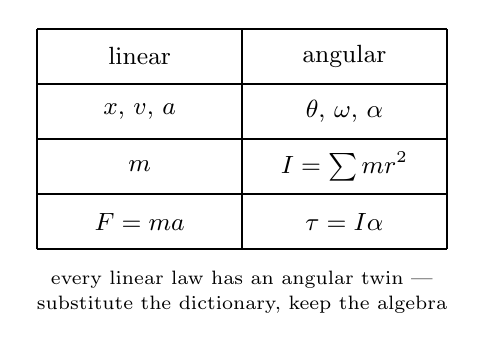
\begin{tikzpicture}[font=\small]
\draw[thick] (0,0) grid[xstep=2.6,ystep=0.7] (5.2,2.8);
\node at (1.3,2.45) {linear};\node at (3.9,2.45) {angular};
\node at (1.3,1.75) {$x$, $v$, $a$};\node at (3.9,1.75) {$\theta$, $\omega$, $\alpha$};
\node at (1.3,1.05) {$m$};\node at (3.9,1.05) {$I=\sum mr^{2}$};
\node at (1.3,0.35) {$F=ma$};\node at (3.9,0.35) {$\tau=I\alpha$};
\node[align=center] at (2.6,-0.55) {\scriptsize every linear law has an angular twin ---\\[-2pt]\scriptsize substitute the dictionary, keep the algebra};
\end{tikzpicture}

\caption{The linear--angular dictionary. Every equation in this chapter is
a ch1--ch2 equation with the entries swapped.}
\label{fig:dict}
\end{figure}

\section{Angular variables}\label{sec:rot-kin}

$\theta$ in radians, $\omega=\dot\theta$, $\alpha=\dot\omega$ --- and the
same constant-acceleration formulas of \S1.3 carry over verbatim:
$\omega=\omega_0+\alpha t$, $\theta=\theta_0+\omega_0t+\tfrac12\alpha t^{2}$,
$\omega^{2}=\omega_0^{2}+2\alpha\Delta\theta$. The rim variables are the
bridge: $v=\omega r$, $a_{\rm tan}=\alpha r$.

\section{Rolling kinematics: the no-slip constraint}\label{sec:rot-noslip}

A wheel rolling without slipping has $v_{\rm cm}=\omega r$ --- the contact
point is instantaneously at rest while the top moves at $2v$
(figure~\ref{fig:rolling}). The constraint is \emph{kinematic}, not
energetic: static friction enforces it without doing work, which is why
rolling races (ch6) are energy problems.

\begin{figure}[htbp]\centering
\begin{tikzpicture}[scale=1.0,force/.style={->,thick,accent}]
\draw[thick] (-0.5,0) -- (4.5,0);
\draw[thick] (2,1) circle (1);
\fill (2,1) circle (0.04) node[above left=-2pt,font=\scriptsize]{C};
\draw[force] (2,1) -- (3.3,1) node[right,font=\scriptsize]{$v$};
\draw[force] (2,2) -- (4.6,2) node[right,font=\scriptsize]{top: $2v$};
\draw[force] (2,0) -- (1.3,0) node[below,font=\scriptsize]{contact: $0$};
\draw[force] (3,1) -- (3.9,1.7) node[right,font=\scriptsize]{};
\node[font=\scriptsize] at (4.0,0.4) {$v=\omega r$ no-slip};
\draw[->,dashed] (2.6,1.4) arc (30:-60:0.55);
\node[font=\scriptsize] at (3.2,1.55) {$\omega$};
\end{tikzpicture}

\caption{Velocity field of a rolling wheel: centre at $v$, top at $2v$,
contact at $0$. Notice the contact point is a usable pivot for one
instant --- the seed of the instantaneous-axis trick.}
\label{fig:rolling}
\end{figure}

\section{Torque: force's lever-arm price}\label{sec:rot-torque}

\begin{equation}
  \boldsymbol\tau=\mathbf r\times\mathbf F,\qquad
  \tau=rF\sin\phi=\ell F,\label{eq:tau}
\end{equation}
where $\ell$ is the \emph{lever arm}\index{lever arm}: the perpendicular
distance from the pivot to the force's line of action
(figure~\ref{fig:torque}). Convention in this book: counterclockwise
positive. Torque is the quantity the door handle sells --- same force,
longer $\ell$, more angular acceleration.

\begin{figure}[htbp]\centering
\begin{tikzpicture}[scale=1.1,force/.style={->,thick,accent}]
\fill (0,0) circle (0.05) node[below left,font=\scriptsize]{pivot};
\draw[thick] (0,0) -- (3.5,0.9);
\draw[force] (3.5,0.9) -- (4.2,2.2) node[right,font=\scriptsize]{$\mathbf F$};
\draw[dashed] (0,0) -- (3.97,1.35);
\draw[dashed,amber] (0,0) -- (2.9,2.1) node[midway,above,font=\scriptsize]{$\ell$};
\draw[thick,amber] (2.9,2.1) -- (4.0,2.24);
\node[font=\scriptsize] at (1.7,0.7) {$\mathbf r$};
\node[font=\scriptsize,align=left] at (5.0,0.3) {$\tau=rF\sin\phi$\\$=\ell F$};
\draw[->,dashed] (0.8,0.35) arc (15:40:0.9);
\node[font=\scriptsize] at (1.15,0.75) {$\phi$};
\end{tikzpicture}

\caption{Torque geometry: $\tau=rF\sin\phi$, equivalently $\ell F$ with the
lever arm $\ell$. Notice only the perpendicular component of $\mathbf F$
pays.}
\label{fig:torque}
\end{figure}

\section{Moment of inertia: mass with an $r^{2}$ tax}\label{sec:rot-i}

\begin{equation}
  I=\sum_i m_ir_i^{2}\;\xrightarrow{\ \text{continuous}\ }\;
  I=\int r^{2}\,dm.\label{eq:moi}
\end{equation}
The $r^{2}$ is the whole story: mass near the axis is cheap, mass at the
rim is expensive --- a hoop resists twice as hard per kilogram as a disk.
Two theorems do most of the work: the \emph{parallel-axis} shift
$I=I_{\rm cm}+Md^{2}$, and the \emph{perpendicular-axis}
$I_z=I_x+I_y$ for flat laminas.

\begin{example}[$I$ of a rod and a disk by direct integration]\label{ex:moi}
Compute $I$ about the centre for (a) a uniform rod of length $L$, (b) a
uniform disk of radius $R$.
\par\smallskip
\textbf{Strategy.} Slice into rings/strips where $r$ is constant; the
integral is bookkeeping, not calculus difficulty.
\begin{solution}
(a) Rod: $dm=\lambda dx$ with $\lambda=M/L$:
$I=\int_{-L/2}^{L/2}x^{2}\lambda\,dx=\lambda\frac{L^{3}}{12}
=\frac{1}{12}ML^{2}$.
(b) Disk: rings of mass $dm=\sigma\,2\pi r\,dr$, all points at the same
$r$: $I=\int_0^{R}r^{2}\sigma2\pi r\,dr
=2\pi\sigma R^{4}/4=\frac{1}{2}MR^{2}$ using
$M=\sigma\pi R^{2}$. \checkmark
\end{solution}
\end{example}

\begin{figure}[htbp]\centering
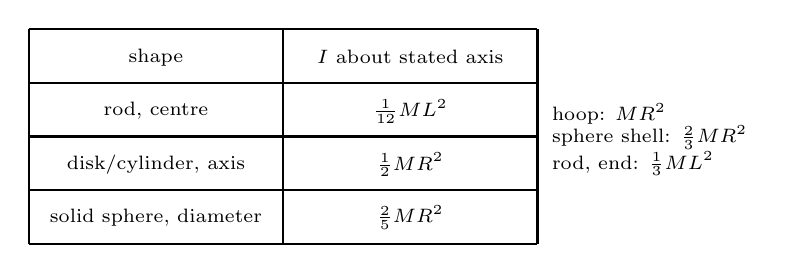
\begin{tikzpicture}[font=\scriptsize,scale=0.95]
\draw[thick] (0,0) grid[xstep=3.4,ystep=0.72] (6.8,2.88);
\node at (1.7,2.5) {shape};\node at (5.1,2.5) {$I$ about stated axis};
\node at (1.7,1.78) {rod, centre};\node at (5.1,1.78) {$\frac{1}{12}ML^{2}$};
\node at (1.7,1.06) {disk/cylinder, axis};\node at (5.1,1.06) {$\frac{1}{2}MR^{2}$};
\node at (1.7,0.36) {solid sphere, diameter};\node at (5.1,0.36) {$\frac{2}{5}MR^{2}$};
\node[align=left] at (8.3,1.4) {hoop: $MR^{2}$\\sphere shell: $\frac{2}{3}MR^{2}$\\rod, end: $\frac{1}{3}ML^{2}$};
\end{tikzpicture}

\caption{The six standard moments. Notice the coefficient tracks how far
mass sits from the axis --- the rod's $1/12$, the disk's $1/2$, the
hoop's $1$.}
\label{fig:itable}
\end{figure}

\begin{lstlisting}[language=Python,caption={\texttt{code/ch05\_inertia\_integrator.py} --- grid quadrature vs analytic $I$; the parallel-axis term on display.},label={lst:moi}]
s += r*r * r*dr*dth   # r^2 * dA, dA = r dr dth
\end{lstlisting}

Output of a real run:
\begin{lstlisting}[numbers=none]
rectangle 2.0x1.0: numeric I=0.8333, exact=0.8333, err=0.00%
  per unit mass: I/M=0.4167 vs (a^2+b^2)/12=0.4167
disk R=1.0: numeric I=1.5708, exact=1.5708, err=0.00%
  per unit mass: I/M=0.5000 vs R^2/2=0.5000
disk about rim: I=4.7124 = I_cm + M R^2 (1.5708 + 3.1416); ratio to I_cm = 3.00
\end{lstlisting}

Notice the last line: spinning a disk about a point on its rim costs
\emph{three times} the centre-axis moment --- the $Md^{2}$ term, not a
numerical artifact.

\section{$\tau=I\alpha$: the massive pulley}\label{sec:rot-tia}

With a real pulley the rope's two sides can't share a tension --- the
difference is what spins the wheel (figure~\ref{fig:pulley}).

\begin{figure}[htbp]\centering
\begin{tikzpicture}[scale=1.0,force/.style={->,thick,accent}]
\draw[thick] (-1.5,3.2) -- (1.5,3.2);
\draw[fill=gray!30] (0,3.2) circle (0.4);
\fill (0,3.2) circle (0.03);
\node[font=\scriptsize] at (0,3.85) {$I=\tfrac12MR^{2}$};
\draw (-0.4,3.2) -- (-0.4,1.2); \draw (0.4,3.2) -- (0.4,0.4);
\filldraw[fill=gray!20] (-0.75,0.7) rectangle (-0.05,1.2);
\node[font=\scriptsize] at (-0.4,0.95) {$m_1$};
\filldraw[fill=gray!20] (0.05,0.0) rectangle (0.75,0.4);
\node[font=\scriptsize] at (0.4,0.2) {$m_2$};
\draw[force] (-0.4,0.7) -- (-0.4,-0.15) node[below,font=\scriptsize]{$m_1g$};
\draw[force] (-0.4,1.2) -- (-0.4,2.0) node[above,font=\scriptsize]{$T_1$};
\draw[force] (0.4,0.0) -- (0.4,-0.85) node[below,font=\scriptsize]{$m_2g$};
\draw[force] (0.4,0.4) -- (0.4,1.3) node[above,font=\scriptsize]{$T_2$};
\node[font=\scriptsize,align=left] at (2.3,1.2) {$T_1\neq T_2$:\\the difference\\spins the pulley};
\end{tikzpicture}

\caption{The massive pulley's three-body problem: two hanging FBDs plus
$\sum\tau=I\alpha$ on the wheel. The tension \emph{difference} does the
spinning.}
\label{fig:pulley}
\end{figure}

\begin{example}[Atwood with a massive pulley]\label{ex:mpulley}
Repeat example 2.1's Atwood ($m_1=3$, $m_2=5$\,kg) with a pulley of mass
$M=4$\,kg, radius $R$, modeled as a disk ($I=\tfrac12MR^{2}$).
\par\smallskip
\textbf{Strategy.} Three equations: two translations plus one rotation.
Constraint: $\alpha=a/R$ (no slip on the rim).
\begin{solution}
$m_2g-T_2=m_2a$, $T_1-m_1g=m_1a$, and
$(T_2-T_1)R=I\alpha=\tfrac12MR^{2}\cdot a/R \Rightarrow T_2-T_1=\tfrac12Ma$.
Adding all three:
\[
  a=\frac{(m_2-m_1)g}{m_1+m_2+M/2}
   =\frac{2\times9.8}{3+5+2}=1.96\,\mathrm{m/s^{2}},
\]
down from $2.45$ --- the pulley acts like an extra $2$\,kg of inertia.
$T_1=35.3$\,N, $T_2=39.2$\,N: no longer equal, and their difference
$3.9$\,N is exactly $\tfrac12Ma$. \checkmark
\end{solution}
\end{example}

\begin{example}[Yo-yo unwinding]\label{ex:yoyo}
A yo-yo (disk, $I=\tfrac12mR^{2}$, string wrapped at radius $r$) falls
unwinding. Find its acceleration.
\par\smallskip
\textbf{Strategy.} Two equations: $mg-T=ma$ and $Tr=I\alpha$ with
$\alpha=a/r$.
\begin{solution}
$T=I a/r^{2}=\tfrac12mR^{2}a/r^{2}$, so
$a=\frac{g}{1+R^{2}/(2r^{2})}$. For $R/r=5$: $a=g/13.5=0.73$\,m/s$^{2}$
--- the rim-radius leverage makes it a slow fall. \checkmark
\end{solution}
\end{example}

\begin{exercise}[medium]
Find $a$ for the yo-yo when it's a hoop ($I=mR^{2}$) instead. (F=ma)
\end{exercise}

\section{Statics: two balances, one smart pivot}\label{sec:rot-static}

Static equilibrium needs $\sum\mathbf F=0$ \emph{and}
$\sum\boldsymbol\tau=0$ --- and the pivot for the second equation is
\emph{yours to choose}: put it where an unknown force acts and that force
disappears from the torque books. That single trick solves most of the
chapter's problems.

\begin{example}[Ladder minimum angle]\label{ex:ladder}
A uniform ladder of length $L$ leans at angle $\theta$ against a
frictionless wall (figure~\ref{fig:ladder}); the floor has $\mu_s$.
Minimum $\theta$ before slipping?
\par\smallskip
\textbf{Strategy.} $\sum F$: $N_2=f$, $N_1=mg$. Torque about the base
(kills $f$ and $N_1$): the wall's push at the top balances gravity at the
middle.
\begin{solution}
$N_2 L\sin\theta=mg\frac{L}{2}\cos\theta \Rightarrow
N_2=\frac{mg}{2\tan\theta}$. Slip when $f=N_2=\mu_sN_1=\mu_smg$:
$\tan\theta_{\min}=\frac{1}{2\mu_s}$. For $\mu_s=0.4$: $\theta_{\min}=
51.3^{\circ}$ --- below that, the wall can't push hard enough. \checkmark
\end{solution}
\end{example}

\begin{figure}[htbp]\centering
\begin{tikzpicture}[scale=1.0,force/.style={->,thick,accent}]
\draw[thick] (0,0) -- (0,4); \draw[thick] (0,0) -- (3.5,0);
\draw[very thick] (0,0.2) -- (2.6,3.8);
\fill (1.3,2.0) circle (0.06);
\draw[force] (1.3,2.0) -- (1.3,0.9) node[right,font=\scriptsize]{$mg$};
\draw[force] (0,0.2) -- (0.7,0.2) node[right,font=\scriptsize]{$f$};
\draw[force] (0,0.2) -- (0,0.95) node[above,font=\scriptsize]{$N_1$};
\draw[force] (2.6,3.8) -- (1.9,3.8) node[left,font=\scriptsize]{$N_2$};
\draw (0.55,0) arc (0:55:0.55); \node[font=\scriptsize] at (0.8,0.35) {$\theta$};
\node[font=\scriptsize,align=left] at (4.3,3.0) {smart pivot: base ---\\kills $f$ and $N_1$};
\end{tikzpicture}

\caption{Ladder FBD: frictionless wall means $N_2$ is purely horizontal;
taking torques about the base deletes both floor forces.}
\label{fig:ladder}
\end{figure}

\begin{exercise}[easy]
Where does a second person standing halfway up the ladder change the
minimum angle? Set up the new torque equation. (AP-C)
\end{exercise}

\begin{example}[Two-support beam]\label{ex:beam}
A uniform $8$\,kg, $5$\,m beam rests on supports at $x=1$ and $x=4$
(metres from the left end), with a $20$\,kg toolbox at $x=4.5$. Find each
support's force.
\par\smallskip
\textbf{Strategy.} $\sum F$ gives the sum; torque about one support kills
its unknown. Watch: the toolbox overhangs the right support.
\begin{solution}
$N_A+N_B=mg+Mg=78.4+196=274.4$\,N.
Torque about support $A$ (CCW$+$): the beam's weight acts at $x=2.5$
(1.5\,m right of $A$), the toolbox at $3.5$\,m right, $N_B$ at $3$\,m:
$3N_B=78.4\times1.5+196\times3.5=117.6+686$, so $N_B=267.9$\,N and
$N_A=6.5$\,N --- the left support nearly unloads: shift the toolbox a
little further and the beam tips. \checkmark
\end{solution}
\end{example}

\section{Rotational kinetic energy}\label{sec:rot-ke}

$K_{\rm rot}=\tfrac12I\omega^{2}$, and for rolling
$K=\tfrac12mv^{2}+\tfrac12I\omega^{2}$ --- the reason a hoop loses every
race down an incline: it pays the rotation tax with the largest per-mass
$I$ (chapter~6 races them properly).

\section{In engineering practice: torque specs}\label{sec:rot-eng}

Every bolt in a car has a printed torque spec --- this chapter's
$\tau=\ell F$ run as quality control: a $25$\,N\,m spec on a $0.25$\,m
wrench means exactly $100$\,N of hand force, and overtightening stretches
the bolt past its elastic range (book5's materials chapter has the yield
story). The statics side is how cranes stay up: $\sum\tau=0$ about the
outrigger line is the tip-over condition, which is why load charts shrink
with boom extension --- longer $\ell$, same budget.

\section{Common mistakes}\label{sec:rot-mistakes}

\begin{tripwire}[Lever arm vs point distance]
$\tau=\ell F$: $\ell$ is perpendicular distance to the \emph{line of
action}, not to the point of application along the body.
\end{tripwire}
\begin{tripwire}[Forgetting the pulley's inertia]
A massless pulley shares one $T$; a massive one doesn't --- drop the
$\tfrac12Ma$ term and the answer is too fast.
\end{tripwire}
\begin{tripwire}[Wrong parallel-axis shift]
$I=I_{\rm cm}+Md^{2}$ --- it's about the CM plus a shift, never between
two arbitrary axes.
\end{tripwire}
\begin{tripwire}[Bad torque origin]
Every force through the origin drops out. Pick the pivot at the unknown
you want gone, not at the centre because it looks official.
\end{tripwire}
\begin{tripwire}[Force balance alone in statics]
$\sum F=0$ admits a whole family of torques; the ladder needs
$\sum\tau=0$ too.
\end{tripwire}

\section{Summary}\label{sec:rot-summary}

\begin{table}[ht]\centering
\begin{tabularx}{\linewidth}{@{}lY@{}}
\toprule
\tablehead\thead{Idea} & \thead{One-line version}\\
\midrule
dictionary & $\theta/\omega/\alpha \leftrightarrow x/v/a$; same formulas \\
no-slip & $v_{\rm cm}=\omega r$; contact instant rest, top $2v$ \\
torque & $\tau=rF\sin\phi=\ell F$; CCW positive \\
moment of inertia & $I=\int r^{2}dm$; $1/12$, $1/2$, $2/5$ coefficients \\
dynamics & $\tau=I\alpha$; massive pulleys need $T_1\neq T_2$ \\
statics & $\sum F=0$ + $\sum\tau=0$; pivot at the unknown \\
rotational $K$ & $\tfrac12I\omega^{2}$; rolling pays both \\
\bottomrule
\end{tabularx}
\caption{Rotation-I cheat sheet.}
\label{tab:rotsummary}
\end{table}

\begin{wins}[Definition of done]
You can now: run the linear--angular dictionary; read a rolling wheel's
velocity field; compute lever arms and torques; integrate $I$ for simple
shapes and apply parallel axis; solve massive-pulley and yo-yo dynamics;
and set up statics with the smart-pivot trick.
\end{wins}

\chapternotes{%
The dictionary-first approach follows MIT 8.01SC weeks 6 and 10--11
\cite{ocw801} and AP Physics C unit 5 \cite{apced}. OpenStax College
Physics ch.~10, 12 \cite{openstax1} covers the same ground; the ladder and
pulley problems are Morin chs.~7--8 \cite{morin} classics. The I-table
coefficients are standard; the quadrature listing checks two of them
numerically.}

\begin{rulebox}[{Watch instead}]
\begin{enumerate}
\item \emph{Rotating Objects, Moment of Inertia, Rotational KE, Neutron
Stars} --- Walter Lewin, MIT 8.01x Lecture 19, 41:00,
\url{https://youtu.be/fDJeVR0o__w} --- \S\ref{sec:rot-i}--\S\ref{sec:rot-ke}
at full length (accessed 2026-10-11).
\item \emph{Angular motion variables} --- Khan Academy Physics, 12:50,
\url{https://youtu.be/garegCgMxxg} --- \S\ref{sec:rot-kin}--\S\ref{sec:rot-noslip}
worked quickly (accessed 2026-10-11).
\end{enumerate}
\end{rulebox}

\section*{Further reading}
\addcontentsline{toc}{section}{Further reading}

\begin{itemize}
\item MIT OpenCourseWare, \emph{8.01SC Classical Mechanics}, weeks 6,
10--11 --- rotation and statics with recitation solutions. At
\url{https://ocw.mit.edu}, course ``8.01SC'' (verified 2026-10-11).
\item OpenStax, \emph{College Physics 2e}, ch.~10 ``Rotational Motion''
and ch.~12 ``Statics'' --- free text at \url{https://openstax.org}
(verified 2026-10-11).
\item College Board, \emph{AP Physics C: Mechanics CED}, Unit 5 --- the
exam blueprint for rotation. At \url{https://apstudents.collegeboard.org}
(verified 2026-10-11).
\item D.~Morin, \emph{Introduction to Classical Mechanics}, chs.~7--8 ---
statics and rotation at the harder level; ISBN 978-0521876223.
\item The Physics Classroom, \emph{Rotational Motion} tutorials ---
readable remediation for \S\ref{sec:rot-kin}--\S\ref{sec:rot-static}, at
\url{https://www.physicsclassroom.com} (verified 2026-10-11).
\item Khan Academy, \emph{Moments, torque, and angular momentum} ---
drills matching the whole chapter, at
\url{https://www.khanacademy.org} under Science $\to$ Physics (verified
2026-10-11).
\end{itemize}

\section*{Additional exercises}
\addcontentsline{toc}{section}{Additional exercises}

\begin{exercise}[easy]
A wheel spins up to $1200$\,rpm in $4$\,s at constant $\alpha$. Find
$\alpha$ in $\mathrm{rad/s^{2}}$ and the angle turned. (AP-C)
\end{exercise}
\begin{exercise}[easy]
Identify the lever arm: a $0.5$\,m wrench at $60^{\circ}$ to a $100$\,N
force --- compute $\tau$ both as $rF\sin\phi$ and $\ell F$. (AP-C)
\end{exercise}
\begin{exercise}[easy]
Write down $I$ for a $2$\,kg, $0.3$\,m-radius disk about its axis and
about a rim point, citing the theorem used. (AP-C)
\end{exercise}
\begin{exercise}[easy]
A uniform beam of length $4$\,m is pinned at one end and carries a
$200$\,N load at its far end. What vertical force at the midpoint holds
it level (neglecting the beam's weight)? (F=ma)
\end{exercise}
\begin{exercise}[easy]
A see-saw: $30$\,kg child at $1.5$\,m left of the pivot balances a
$50$\,kg adult. Where does the adult sit? (F=ma)
\end{exercise}
\begin{exercise}[medium]
Massive-pulley Atwood: recompute example~\ref{ex:mpulley} with a hoop
pulley ($I=MR^{2}$) --- which way does $a$ move, and why? (F=ma classic)
\end{exercise}
\begin{exercise}[medium]
Redo example~\ref{ex:ladder} with a wall that has $\mu_s'=0.3$ of its
own. Does the wall friction help or hurt? (AP-C FR-style)
\end{exercise}
\begin{exercise}[medium]
A yo-yo hoop ($I=mR^{2}$, string at $r$) falls unwinding --- find $a$
and compare with example~\ref{ex:yoyo}. (F=ma)
\end{exercise}
\begin{exercise}[medium]
Composite body: a $0.5$\,m rod of mass $2$\,kg has a $1$\,kg,
$0.1$\,m-radius disk welded at one end (disk axis through the rod's end,
perpendicular). Find $I$ about the rod's other end. (AP-C)
\end{exercise}
\begin{exercise}[medium]
Sign-of-torque reasoning: a door pushed at its top vs its middle, same
force --- describe the angular acceleration ratio without computing.
(AP-C)
\end{exercise}
\begin{exercise}[medium]
Rolling preview: a hoop and a disk race down an incline from rest ---
predict the winner using only the $I$ coefficients, then verify with
energy ($v^{2}=\frac{2gh}{1+I/mr^{2}}$). (AP-C)
\end{exercise}
\begin{exercise}[medium]
A uniform $8$\,kg beam $5$\,m long rests on two supports at $x=1$ and
$x=4$ (metres). Find each reaction force. (F=ma)
\end{exercise}
\begin{exercise}[hard]
A uniform rod leans on a frictionless floor against a frictionless wall
and is released. Show it loses wall contact when
$\sin\theta=\frac{2}{3}\sin\theta_0$ --- use energy for speed and the CM's
horizontal acceleration for the contact condition. (USAPhO-style)
\end{exercise}
\begin{exercise}[hard]
A rod of length $L$ has density $\lambda(x)=\lambda_0(1+x/L)$. Find its
$I$ about the light end by direct integration, and its CM. (APhO-style)
\end{exercise}
\begin{exercise}[medium]
A sphere and a cylinder of the same $M$, $R$ roll (not slide) down the
same incline. Using $v^{2}=\frac{2gh}{1+I/mr^{2}}$, find the sphere's
speed advantage over the cylinder's at the bottom as a percentage.
(AP-C)
\end{exercise}

\chapter{Rotation II: angular momentum and rolling}\label{ch:rot2}

Linear momentum had its chapter; angular momentum is its equal partner ---
the second conserved quantity of mechanics and the reason gyroscopes,
planets, and skaters behave the way they do. The bookkeeping mirrors
chapter~3 exactly, with one new subtlety: the origin you measure from
matters.

\section{Angular momentum: definition}\label{sec:ang-l}

For a particle,
\begin{equation}
  \mathbf L=\mathbf r\times\mathbf p\label{eq:ldef}
\end{equation}
--- momentum filtered through the position relative to a chosen origin
(figure~\ref{fig:lvec}). A straight-line mover carries nonzero $\mathbf L$
about any origin off its line --- the quantity is about the
\emph{rotation of the line of sight}, not about actual circling.

\begin{figure}[htbp]\centering
\begin{tikzpicture}[scale=1.1,force/.style={->,thick,accent}]
\fill (0,0) circle (0.05) node[below left,font=\scriptsize]{origin};
\draw[force] (0,0) -- (3,1.2) node[midway,below,font=\scriptsize]{$\mathbf r$};
\fill (3,1.2) circle (0.05);
\draw[force] (3,1.2) -- (4.5,0.9) node[right,font=\scriptsize]{$\mathbf p$};
\draw[dashed] (3,1.2) -- (4.3,1.72);
\draw[dashed,amber] (0,0) -- (2.6,1.04);
\draw[->,very thick,amber] (1.5,0.6) -- (1.5,0.1) node[below,font=\scriptsize]{$\mathbf L=\mathbf r\times\mathbf p$};
\node[font=\scriptsize] at (4.8,1.8) {out of page};
\end{tikzpicture}

\caption{$\mathbf L=\mathbf r\times\mathbf p$: magnitude $rp\sin\theta$,
direction by the right-hand rule (out of the page here). Notice it needs an
origin --- the same $\mathbf p$ has different $\mathbf L$ about different
points.}
\label{fig:lvec}
\end{figure}

\section{Rigid bodies: when $L=I\omega$ holds}\label{sec:ang-rigid}

Summing \eqref{eq:ldef} over a rigid body rotating about a fixed
symmetry axis gives
\[
  L=I\omega.
\]
The fine print: valid about the fixed axis \emph{or} about the CM --- the
two origins where the cross terms vanish. A rolling wheel's $\mathbf L$ is
$I\omega$ about its CM \emph{plus} the orbital $M(\mathbf R\times\mathbf V)$
of the CM --- both exist, both count.

\section{The rotational second law}\label{sec:ang-taul}

\begin{equation}
  \boldsymbol\tau_{\rm ext}=\frac{d\mathbf L}{dt}\label{eq:taul}
\end{equation}
about an inertial fixed point or about the CM --- the two origins where the
derivation works. Choosing an accelerating origin is the classic trap: the
equation picks up fictitious-torque terms that ruin it.

\section{Conservation of angular momentum}\label{sec:ang-cons}

\begin{principle}[Angular momentum conservation]
$\mathbf L$ is conserved when the net \emph{external torque} is zero ---
weaker than zero external force. A planet feels a huge central force that
exerts no torque, so its $\mathbf L$ (and Kepler's second law) survives.
\end{principle}

\begin{example}[The skater]\label{ex:skater}
A skater spins at $\omega_0=2$\,rad/s with $I_0=3$\,kg\,m$^{2}$, then pulls
her arms to $I=1$\,kg\,m$^{2}$. Find the new spin rate and the energy
change.
\par\smallskip
\textbf{Strategy.} No external torque about the spin axis: $L$ conserved.
$K$ is not --- her arms do work.
\begin{solution}
$\omega=I_0\omega_0/I=6$\,rad/s. Energies:
$K_0=\tfrac12(3)(4)=6$\,J, $K=\tfrac12(1)(36)=18$\,J --- $K$ tripled. The
extra $12$\,J came from her muscles pulling mass inward against the
centrifugal pull: the audit of ch4 applies here too. \checkmark
\end{solution}
\end{example}

\begin{figure}[htbp]\centering
\begin{tikzpicture}[scale=1.0,font=\scriptsize]
\begin{scope}
\draw[fill=gray!20] (0,0) ellipse (0.25 and 0.7);
\draw[thick] (-0.9,0.3) -- (0.9,0.3);
\draw[thick] (-0.9,0.5) -- (0.9,0.5);
\fill[fill=amber!40] (-1.0,0.2) rectangle (-0.8,0.6);
\fill[fill=amber!40] (0.8,0.2) rectangle (1.0,0.6);
\node at (0,-1.0) {arms out: $I$ big, $\omega$ small};
\draw[->,dashed] (0,-0.7) arc (-90:200:0.4);
\end{scope}
\begin{scope}[xshift=3.6cm]
\draw[fill=gray!20] (0,0) ellipse (0.2 and 0.7);
\draw[thick] (-0.3,0.4) -- (0.3,0.4);
\fill[fill=amber!40] (-0.35,0.25) rectangle (-0.15,0.55);
\fill[fill=amber!40] (0.15,0.25) rectangle (0.35,0.55);
\node at (0,-1.0) {arms in: $I$ small, $\omega$ big};
\draw[->,dashed] (0,-0.7) arc (-90:290:0.3);
\end{scope}
\node at (1.8,-1.9) {$L=I\omega$ fixed; $K=\tfrac12I\omega^{2}$ grows --- the arms' work pays it};
\end{tikzpicture}

\caption{The skater trade: $L$ fixed, $K$ tripled --- arms supply the
difference.}
\label{fig:skater}
\end{figure}

\begin{example}[Bullet into a pivoted rod]\label{ex:bulletrod}
A $10$\,g bullet at $400$\,m/s embeds in the tip of a $1$\,kg,
$1$\,m rod pivoted at its top ($I=\tfrac13ML^{2}$). Find the angular
velocity just after.
\par\smallskip
\textbf{Strategy.} Linear momentum is \emph{not} conserved (the pivot
pushes); angular momentum about the pivot \emph{is} (the pivot force has
no lever arm). Use the collision instant only.
\begin{solution}
$L_i=mvL=0.01\times400\times1=4$\,kg\,m$^{2}$/s.
$I_{\rm tot}=\tfrac13(1)(1)+0.01(1)^{2}=0.343$\,kg\,m$^{2}$.
$\omega=4/0.343=11.7$\,rad/s. $K$ audit: before $800$\,J, after
$\tfrac12I\omega^{2}=23.4$\,J --- $97\%$ lost to the embedding, as
inelastic as collisions get. \checkmark
\end{solution}
\end{example}

\begin{figure}[htbp]\centering
\begin{tikzpicture}[scale=1.0,force/.style={->,thick,accent}]
% bullet embedding in rod
\draw[very thick] (0,0) -- (0,3.2);
\fill (0,2.4) circle (0.05) node[right,font=\scriptsize]{pivot};
\draw[force] (-2.2,2.9) -- (-0.2,2.9) node[left,midway,above,font=\scriptsize]{bullet $\mathbf p$};
\fill[fill=gray!30] (-0.15,2.7) rectangle (0.15,3.1);
\draw[->,dashed] (0.5,2.9) arc (0:120:0.7);
\node[font=\scriptsize] at (1.3,3.4) {$\omega$ after};
\node[font=\scriptsize,align=left] at (3.4,1.4) {$L_{\rm in}=p\,d$ at impact\\$p$ NOT conserved:\\pivot pushes};
\end{tikzpicture}

\caption{Bullet-and-rod: conserve $L$ about the pivot, not $p$ --- the
pivot's impulse is external to translation but torque-free about itself.}
\label{fig:rxp}
\end{figure}

\begin{exercise}[easy]
In example~\ref{ex:bulletrod}, which quantities survive: total $\mathbf L$
about the pivot, total $\mathbf p$, total $K$? One-line each. (AP-C)
\end{exercise}

\section{Rolling dynamics, three ways}\label{sec:ang-roll}

A roller on an incline can be solved by forces and torque
($ma=mg\sin\theta-f$, $I\alpha=fr$), by energy
($v^{2}=2gh/(1+\beta)$ for $I=\beta mr^{2}$), or by the instantaneous-axis
trick (torque about the contact point only). All three agree; the energy
route is the fastest.

\begin{example}[The incline race]\label{ex:race}
Hoop ($\beta=1$), disk ($\tfrac12$) and sphere ($\tfrac25$) race down a
$2$\,m drop. Order and margins?
\par\smallskip
\textbf{Strategy.} $v=\sqrt{2gh/(1+\beta)}$ --- smaller $\beta$ finishes
first, independent of mass and radius.
\begin{solution}
$v_{\rm sph}=5.29$, $v_{\rm disk}=5.11$, $v_{\rm hoop}=4.43$\,m/s ---
the code listing below prints the same numbers. The hoop loses because
\emph{all} its mass sits at the rim: half its energy is rotation at every
instant (figure~\ref{fig:race}). \checkmark
\end{solution}
\end{example}

\begin{figure}[htbp]\centering
\begin{tikzpicture}[scale=0.8,font=\scriptsize]
\foreach \x/\lab/\tr/\rt in {0/slide/4/0, 2.4/sphere/2.85/1.15, 4.8/disk/2.65/1.35, 7.2/hoop/2/2}{
  \begin{scope}[xshift=\x cm]
    \draw[thick] (0,0) rectangle (1.8,2.8);
    \fill[accent!70] (0,0) rectangle (0.8,\tr*0.6);
    \fill[amber!60] (1.0,0) rectangle (1.8,\rt*0.6);
    \node at (0.9,-0.4) {\lab};
    \node[rotate=90] at (0.4,\tr*0.3) {$K_t$};
    \node[rotate=90] at (1.4,\rt*0.3) {$K_r$};
  \end{scope}}
\node at (3.6,3.5) {same $mgh$: rotation share slows the finish --- hoop pays half};
\end{tikzpicture}

\caption{Energy partition in the race: same $mgh$, different splits ---
the hoop spends half on spinning.}
\label{fig:race}
\end{figure}

\begin{lstlisting}[language=Python,caption={\texttt{code/ch06\_rolling\_race.py} --- the incline race for several shape factors.},label={lst:race}]
v = math.sqrt(2*G*H/(1+beta))
\end{lstlisting}

Output of a real run:
\begin{lstlisting}[numbers=none]
incline drop h=2.0 m
shape                   beta   v (m/s)    K_tr   K_rot
point mass (slide)       0.0     6.261   19.60    0.00
solid sphere             0.4     5.292   14.00    5.60
solid disk               0.5     5.112   13.07    6.53
hoop                     1.0     4.427    9.80    9.80

finish order: point mass (slide) > solid sphere > solid disk > hoop
sphere beats hoop by 19.5% of hoop's speed
\end{lstlisting}

Notice the partition column: the hoop's $K_{\rm rot}$ equals its
$K_{\rm tr}$ --- $\beta=1$ means rotation and translation split the
budget evenly, and mass/radius never appear. Figure~\ref{fig:speedbeta}
plots the finish speeds against $\beta$: the points fall exactly on
$v=\sqrt{2gh/(1+\beta)}$, so the whole race reduces to one parameter.

\begin{figure}[htbp]\centering
\begin{tikzpicture}
\begin{axis}[width=8.8cm,height=5.2cm,xlabel={shape factor $\beta$ of $I=\beta mr^{2}$},
ylabel={finish speed (m/s)},
xmin=-0.08,xmax=1.08,ymin=0,ymax=7,font=\small,legend pos=north east,
xtick={0,0.4,0.5,1.0},xticklabels={slide,sphere,disk,hoop}]
\addplot[very thick,accent,mark=*,mark size=2.2pt] coordinates
{(0,6.261) (0.4,5.292) (0.5,5.112) (1.0,4.427)};
\addlegendentry{race simulation}
\addplot[dashed,domain=-0.08:1.08,samples=2] {6.261/sqrt(1+x)};
\node[font=\scriptsize,anchor=west] at (axis cs:0.05,3.6) {$v=\sqrt{2gh/(1+\beta)}$};
\node[font=\scriptsize,accent,anchor=west] at (axis cs:0.42,6.0) {$K_{\rm rot}$ tax grows with $\beta$};
\end{axis}
\end{tikzpicture}

\caption{Finish speed versus the shape factor $\beta$: simulated points
on the analytic curve. Bigger $\beta$ means a bigger rotational tax ---
and nothing else matters.}
\label{fig:speedbeta}
\end{figure}

\begin{example}[Two-disk angular collision]\label{ex:twodisk}
A disk ($I_1=2$\,kg\,m$^{2}$) spinning at $10$\,rad/s drops onto a
stationary disk ($I_2=3$\,kg\,m$^{2}$) on the same axle; friction locks
them. Find the common $\omega$ and the energy lost.
\par\smallskip
\textbf{Strategy.} Angular-momentum conservation about the axle --- the
angular version of the perfectly inelastic collision.
\begin{solution}
$\omega=I_1\omega_0/(I_1+I_2)=20/5=4$\,rad/s.
$K_i=\tfrac12(2)(100)=100$\,J;
$K_f=\tfrac12(5)(16)=40$\,J --- $60\%$ lost, the angular mirror of
chapter 3's inelastic hit. \checkmark
\end{solution}
\end{example}

\begin{example}[Child on a turntable]\label{ex:turntable}
A $40$\,kg child stands at the rim of a $200$\,kg, $3$\,m-radius
turntable ($I=\tfrac12MR^{2}=900$\,kg\,m$^{2}$) spinning at
$\omega_0=0.5$\,rad/s, then walks to the centre. Find the new $\omega$.
\par\smallskip
\textbf{Strategy.} No external torque about the axis: $I\omega$ conserved,
with the child as a point mass whose $I$ shrinks.
\begin{solution}
$I_0=900+40(9)=1260$\,kg\,m$^{2}$; at centre $I_1=900+0$.
$\omega_1=0.5\times1260/900=0.70$\,rad/s --- the same skater effect with
the child playing the arms. $K$ rises from $158$ to $220$\,J, paid by the
child's steps. \checkmark
\end{solution}
\end{example}

\begin{exercise}[medium]
A $40$\,kg child walks from rim to centre on a $200$\,kg, $3$\,m-radius
turntable ($I=\tfrac12MR^{2}$) spinning at $0.5$\,rad/s. Find the new
$\omega$. (AP-C FR-style)
\end{exercise}

\section{Gyroscopic precession: the order of magnitude}\label{sec:ang-gyro}

A spinning top tilted at angle $\theta$ has $\mathbf L$ along its axis;
gravity's torque $\tau=mgd\sin\theta$ is perpendicular, so $\mathbf L$
\emph{rotates} rather than tips (figure~\ref{fig:gyro}). The precession
rate follows from $\Delta L=\tau\Delta t$ geometry:
\[
  \Omega=\frac{\tau}{L}=\frac{mgd}{I\omega}
\]
--- slower spin, faster wobble. That's why tops precess more as they wind
down.

\begin{figure}[htbp]\centering
\begin{tikzpicture}[scale=1.0,force/.style={->,thick,accent}]
\draw[thick] (0,0) -- (2.5,0);
\fill (0,0) circle (0.05) node[below,font=\scriptsize]{pivot};
\draw[thick] (2.5,0) ellipse (0.25 and 0.7);
\draw[force] (2.5,0) -- (2.5,-0.9) node[below,font=\scriptsize]{$mg$};
\draw[force,very thick,amber] (1.2,0) -- (3.2,0) node[right,font=\scriptsize]{$\mathbf L$};
\draw[force,amber] (0,0.3) -- (0,0.9) node[above,font=\scriptsize]{$\boldsymbol\tau$};
\draw[->,dashed] (1.2,-1.6) arc (0:50:1.2) node[midway,right,font=\scriptsize]{precession};
\node[font=\scriptsize,align=left] at (4.6,0.4) {$\Omega=\frac{\tau}{L}$:\\gravity makes\\it precess};
\node[font=\scriptsize,align=left] at (4.6,0.4) {};
\end{tikzpicture}

\caption{Precession bookkeeping: $\boldsymbol\tau$ perpendicular to
$\mathbf L$ turns the vector instead of shrinking it. $\Omega=\tau/L$ sets
the rate.}
\label{fig:gyro}
\end{figure}

\section{In engineering practice: reaction wheels and flywheels}\label{sec:ang-eng}

Satellites steer with \emph{reaction wheels} --- small spun disks whose
speed changes trade $\mathbf L$ with the bus, no fuel spent: this chapter's
conservation law is the whole attitude-control budget. Flywheel energy
storage is the same $K=\tfrac12I\omega^{2}$ as grid batteries: a
$500$\,kg carbon-fiber wheel at $20{,}000$\,rpm banks megajoules in
rotation, which is exactly the hoop's tax of
figure~\ref{fig:race} run to its useful extreme --- mass at the rim is
where you want it.

\section{Common mistakes}\label{sec:ang-mistakes}

\begin{tripwire}[$L=I\omega$ about the wrong axis]
Valid about the fixed axis or the CM only. A rolling wheel about an
arbitrary point needs $I\omega+\mathbf R\times M\mathbf V$.
\end{tripwire}
\begin{tripwire}[Conserving $L$ through external torque]
The bullet-in-rod survives precisely because the pivot torque about the
pivot is zero --- any other origin, or any other external torque, breaks it.
\end{tripwire}
\begin{tripwire}[Forgetting translational $K$ in rolling]
A rolling object carries $\tfrac12mv^{2}+\tfrac12I\omega^{2}$ --- drop the
first term and every race comes out tied.
\end{tripwire}
\begin{tripwire}[$\tau=dL/dt$ about a non-inertial origin]
The law holds at inertial points and the CM. An accelerating origin
invents torques that aren't there.
\end{tripwire}
\begin{tripwire}[Cross-product sign]
$\mathbf r\times\mathbf p\neq\mathbf p\times\mathbf r$ --- the order flips
the sign. Fix the convention once per problem.
\end{tripwire}

\section{Summary}\label{sec:ang-summary}

\begin{table}[ht]\centering
\begin{tabularx}{\linewidth}{@{}lY@{}}
\toprule
\tablehead\thead{Idea} & \thead{One-line version}\\
\midrule
definition & $\mathbf L=\mathbf r\times\mathbf p$ --- origin-dependent \\
rigid body & $L=I\omega$ about fixed axis or CM \\
dynamics & $\boldsymbol\tau=d\mathbf L/dt$ at inertial origin or CM \\
conservation & survives iff external torque $=0$ --- central forces OK \\
rolling & $v^{2}=2gh/(1+\beta)$; smaller $\beta$ wins \\
skater & $L$ fixed, $K$ grows --- muscles pay \\
gyroscope & $\Omega=\tau/L$; perpendicular torque turns, doesn't tip \\
\bottomrule
\end{tabularx}
\caption{Angular momentum cheat sheet.}
\label{tab:angsummary}
\end{table}

\begin{wins}[Definition of done]
You can now: compute $\mathbf L$ for particles and rigid bodies; state
when conservation applies; solve skater, bullet-rod, and two-disk
collisions; run the incline race three ways; and size gyroscopic
precession to order of magnitude.
\end{wins}

\chapternotes{%
The treatment follows MIT 8.01SC weeks 11--12 plus its gyroscope module
\cite{ocw801} and AP Physics C unit 6 \cite{apced}. Morin chs.~8--9
\cite{morin} is the source of the spool and sliding-to-rolling exercises;
OpenStax ch.~11 \cite{openstax1} covers the same material. The race
numbers are the listing's real output.}

\begin{rulebox}[{Watch instead}]
\begin{enumerate}
\item \emph{Angular Momentum, Torques, Conservation of Angular Momentum}
--- Walter Lewin, MIT 8.01x Lecture 20, 51:15,
\url{https://youtu.be/sNaaL19opxw} --- the whole chapter at full length
(accessed 2026-10-11).
\item \emph{Conservation of angular momentum} --- Khan Academy, 7:16,
\url{https://youtu.be/vfmLI150g4w} --- \S\ref{sec:ang-cons} worked quickly
(accessed 2026-10-11).
\end{enumerate}
\end{rulebox}

\section*{Further reading}
\addcontentsline{toc}{section}{Further reading}

\begin{itemize}
\item MIT OpenCourseWare, \emph{8.01SC Classical Mechanics}, weeks 11--12
--- angular momentum and rolling with recitation solutions. At
\url{https://ocw.mit.edu}, course ``8.01SC'' (verified 2026-10-11).
\item OpenStax, \emph{College Physics 2e}, ch.~10--11 --- free text at
\url{https://openstax.org} (verified 2026-10-11).
\item College Board, \emph{AP Physics C: Mechanics CED}, Unit 6 --- the
exam blueprint for angular momentum. At
\url{https://apstudents.collegeboard.org} (verified 2026-10-11).
\item D.~Morin, \emph{Introduction to Classical Mechanics}, chs.~8--9 ---
angular momentum and rolling at the harder level; ISBN 978-0521876223.
\item The Physics Classroom, \emph{Angular Momentum} tutorials --- readable
remediation, at \url{https://www.physicsclassroom.com} (verified
2026-10-11).
\item Khan Academy, \emph{Moments, torque, and angular momentum} ---
drills matching the whole chapter, at \url{https://www.khanacademy.org}
under Science $\to$ Physics (verified 2026-10-11).
\end{itemize}

\section*{Additional exercises}
\addcontentsline{toc}{section}{Additional exercises}

\begin{exercise}[easy]
Find the magnitude and direction of $\mathbf L$ for a $2$\,kg mass at
$\mathbf r=(3,0,0)$\,m moving at $\mathbf v=(0,4,0)$\,m/s. (AP-C)
\end{exercise}
\begin{exercise}[easy]
Decide whether $L$ is conserved in each: (a) planet orbiting the sun,
(b) figure skater pulling in arms, (c) frisbee spinning while gliding to
a stop, (d) the bullet-rod of example~\ref{ex:bulletrod} \emph{after}
impact. (AP-C)
\end{exercise}
\begin{exercise}[easy]
A rolling ball has $v=5$\,m/s and radius $0.1$\,m. Find $\omega$ and
the contact point's instantaneous speed. (AP-C)
\end{exercise}
\begin{exercise}[easy]
Explain in one sentence why the skater's $K$ increases while $L$ stays
fixed. (F=ma)
\end{exercise}
\begin{exercise}[easy]
A spinning disk has $I=0.5$\,kg\,m$^{2}$, $\omega=20$\,rad/s. Find $L$
and $K_{\rm rot}$. (AP-C)
\end{exercise}
\begin{exercise}[medium]
A $40$\,kg child stands at the rim of a $150$\,kg, $4$\,m-radius
turntable ($I=\tfrac12MR^{2}$) at rest, then walks clockwise at
$1$\,m/s relative to the ground. Which way and how fast does the table
turn? (AP-C FR-style)
\end{exercise}
\begin{exercise}[medium]
Rank these down a $3$\,m incline by finish order and compute each speed:
solid sphere, hollow sphere ($\beta=2/3$), disk, hoop. (F=ma)
\end{exercise}
\begin{exercise}[medium]
Example~\ref{ex:bulletrod} with a bullet hitting \emph{halfway} down the
rod: recompute $\omega$ and the energy loss. (AP-C)
\end{exercise}
\begin{exercise}[medium]
Two angular disks merge: $I_1=1$, $\omega_1=12$ and $I_2=4$ spinning
\emph{oppositely} at $\omega_2=-3$. Find the common $\omega$ and energy
lost. (F=ma)
\end{exercise}
\begin{exercise}[medium]
A $0.5$\,m wrench applies $40$\,N tangentially to a $0.02$\,m-radius
shaft. Find the torque and, for a $0.1$\,kg\,m$^{2}$ flywheel, the
$\omega$ after $5$\,s from rest. (AP-C)
\end{exercise}
\begin{exercise}[medium]
A gyroscope with $I=0.01$\,kg\,m$^{2}$, $\omega=200$\,rad/s, $d=0.1$\,m,
$m=0.5$\,kg: compute the precession rate in rad/s and rpm. (F=ma)
\end{exercise}
\begin{exercise}[hard]
A bowling ball is set sliding with no spin at $v_0$ on a lane with
$\mu_k$. Show it transitions to pure rolling at $v=\frac{5}{7}v_0$ ---
track both $v$ and $\omega$ as friction acts. (USAPhO-style)
\end{exercise}
\begin{exercise}[hard]
A spool of thread lies on a table ($I=\beta mr^{2}$, thread wrapped at
inner radius $r_i<R$). Pulling the thread horizontally: does it roll
toward or away from you? Find the critical angle where the direction
reverses. (APhO-style classic)
\end{exercise}
\begin{exercise}[medium]
Energy split check: for the race of example~\ref{ex:race}, what fraction
of each shape's kinetic energy is rotational? Show $\beta/(1+\beta)$.
(AP-C)
\end{exercise}
\begin{exercise}[medium]
A planet at perihelion ($r_1$, $v_1$) reaches aphelion at $2r_1$. Find
its aphelion speed by $L$ conservation, and explain why this is Kepler's
second law. (F=ma)
\end{exercise}

\chapter{Oscillations}\label{ch:osc}

One equation runs this chapter: $\ddot x+\omega_0^{2}x=0$. Springs,
pendulums, RLC circuits (ch15) and molecule vibrations are all its
instances. Add damping and a drive and the same equation explains resonance
--- from tuning forks to the Tacoma bridge.

\section{SHM: the equation and its family}\label{sec:osc-shm}

\begin{equation}
  \ddot x+\omega_0^{2}x=0\;\Rightarrow\;
  x(t)=A\cos(\omega_0t+\phi),\label{eq:shm}
\end{equation}
two constants $A,\phi$ paid by two initial conditions. The frequency
$\omega_0$ is set by the physics; the amplitude is yours. Notice what's
\emph{not} in the solution: $A$ never changes the period --- the signature
of a linear restoring force.

\section{Spring--mass: the canonical case}\label{sec:osc-spring}

$-kx=m\ddot x$ gives $\omega_0=\sqrt{k/m}$ and
$T=2\pi\sqrt{m/k}$: stiffer is faster, heavier is slower. Energy trades
$\tfrac12kx^{2}$ and $\tfrac12mv^{2}$ with
$E=\tfrac12kA^{2}$ --- quadratic in amplitude, so doubling $A$ quadruples
the energy.

\begin{example}[Energy split in a spring oscillator]\label{ex:springE}
A $0.5$\,kg mass on a $200$\,N/m spring oscillates with $A=0.15$\,m.
Find $E$, $v_{\max}$, and the speed at $x=A/2$.
\par\smallskip
\textbf{Strategy.} $E$ is set by amplitude; at any $x$ the remainder
after $\tfrac12kx^{2}$ is kinetic.
\begin{solution}
$E=\tfrac12(200)(0.0225)=2.25$\,J;
$v_{\max}=\sqrt{2E/m}=\sqrt{9}=3$\,m/s at centre.
At $x=0.075$: $U=\tfrac12(200)(0.0056)=0.56$\,J, so
$v=\sqrt{2(2.25-0.56)/0.5}=2.6$\,m/s --- three quarters of max at half
amplitude: energy spends most of the cycle near the turning points.
\checkmark
\end{solution}
\end{example}

\section{Pendulums: small-angle as an approximation with a limit}\label{sec:osc-pend}

For a pendulum the restoring torque is $-mgL\sin\theta$
(figure~\ref{fig:pend}); linearising $\sin\theta\approx\theta$ gives
$\omega_0=\sqrt{g/L}$ --- good to $1\%$ for
$\theta_0\lesssim23^{\circ}$, and the first correction
$T\approx T_0(1+\theta_0^{2}/16)$ is the hard exercise at the end.
A physical pendulum generalises it:
$\omega_0=\sqrt{mgd/I}$.

\begin{figure}[htbp]\centering
\begin{tikzpicture}[scale=1.2,force/.style={->,thick,accent}]
\fill (0,0) circle (0.04) node[above,font=\scriptsize]{pivot};
\draw[thick] (0,0) -- (1.8,-2.5);
\fill[fill=gray!30] (1.8,-2.5) circle (0.12);
\draw[dashed] (0,0) -- (0,-2.7);
\draw[force] (1.8,-2.5) -- (1.8,-3.4) node[below,font=\scriptsize]{$mg$};
\draw[force,dashed,amber] (1.8,-2.5) -- (1.1,-2.95) node[left,font=\scriptsize]{$mg\sin\theta$};
\draw (0.55,0) arc (0:-54:0.55);
\node[font=\scriptsize] at (0.85,-0.45) {$\theta$};
\node[font=\scriptsize,align=left] at (2.6,-1.5) {restore $\approx-mg\theta$\\for $\theta\lesssim15^{\circ}$};
\node[font=\scriptsize,align=left] at (2.6,-1.5) {};
\end{tikzpicture}

\caption{The pendulum's restoring force $-mg\sin\theta$ is \emph{almost}
linear --- small-angle is an approximation with a budget, not a property.}
\label{fig:pend}
\end{figure}

\begin{example}[Meter-stick physical pendulum]\label{ex:physpend}
A uniform meter stick pivots at one end. Find its period.
\par\smallskip
\textbf{Strategy.} Physical pendulum: $\omega_0^{2}=mgd/I$ with $d=L/2$,
$I=\tfrac13mL^{2}$.
\begin{solution}
$\omega_0^{2}=\frac{g(L/2)}{L^{2}/3}=\frac{3g}{2L}$, so
$T=2\pi\sqrt{\frac{2L}{3g}}=2\pi\sqrt{\frac{2}{29.4}}=1.64$\,s. A simple
pendulum this long would take $2.0$\,s --- the stick's spread mass makes
it faster. \checkmark
\end{solution}
\end{example}

\section{Damped oscillations: three regimes}\label{sec:osc-damped}

Add $-b\dot x$: $\ddot x+\gamma\dot x+\omega_0^{2}x=0$ with
$\gamma=b/m$. The discriminant sorts the behaviour
(figure~\ref{fig:damp}): \textbf{underdamped} ($\gamma<2\omega_0$)
oscillates inside an $e^{-\gamma t/2}$ envelope at
$\omega_d=\sqrt{\omega_0^{2}-\gamma^{2}/4}$; \textbf{critical}
($\gamma=2\omega_0$) returns fastest without ringing;
\textbf{overdamped} ($\gamma>2\omega_0$) creeps back slowly. Car
suspension and door closers are engineered to sit just under critical.

\begin{figure}[htbp]\centering
\begin{tikzpicture}
\begin{axis}[width=9cm,height=5cm,xlabel={$t$},ylabel={$x$},
xmin=0,xmax=20,ymin=-1.3,ymax=1.3,xtick={0,5,10,15,20},font=\small,legend pos=north east]
\addplot[very thick,accent,domain=0:20,samples=120] {exp(-0.08*x)*cos(deg(2*x))};
\addlegendentry{under}
\addplot[very thick,amber,domain=0:20,samples=60] {exp(-0.5*x)*cos(deg(1.6*x))};
\addlegendentry{critical-ish}
\addplot[very thick,dashed,domain=0:20,samples=60] {exp(-0.9*x)};
\addlegendentry{over}
\end{axis}
\end{tikzpicture}

\caption{The three damping regimes. Notice only the underdamped case
crosses zero --- the others surrender exponentially.}
\label{fig:damp}
\end{figure}

\begin{example}[Extracting the constants from a trace]\label{ex:damped}
A decaying trace shows maxima at $1.00$, $0.82$, $0.67$ at $t=0$, $2.1$,
$4.2$\,s. Find $\gamma$, $\omega_d$, $\omega_0$.
\par\smallskip
\textbf{Strategy.} Envelope ratio per period gives $\gamma$; the period
gives $\omega_d$; the relation $\omega_d^{2}=\omega_0^{2}-\gamma^{2}/4$
closes it.
\begin{solution}
Period $T_d\approx2.1$\,s $\Rightarrow\omega_d=2.99$\,rad/s.
Ratio per period $0.82$: $e^{-\gamma T_d/2}=0.82 \Rightarrow
\gamma=0.19$\,s$^{-1}$.
$\omega_0=\sqrt{\omega_d^{2}+\gamma^{2}/4}=\sqrt{8.94+0.009}=2.99$\,rad/s
--- damping barely shifts the frequency here. \checkmark
\end{solution}
\end{example}

\begin{exercise}[easy]
Show the same trace's next two maxima and estimate them. (AP-C)
\end{exercise}

\section{Driven oscillations and resonance}\label{sec:osc-driven}

A drive $F_0\cos\omega_dt$ produces steady amplitude
\begin{equation}
  A(\omega_d)=\frac{F_0/m}{\sqrt{(\omega_0^{2}-\omega_d^{2})^{2}
  +(\gamma\omega_d)^{2}}},\label{eq:amp}
\end{equation}
peaking near $\omega_d=\sqrt{\omega_0^{2}-\gamma^{2}/2}$
(figure~\ref{fig:resonance}). The peak height is set by the
\emph{quality factor} $Q=\omega_0/\gamma$: high-$Q$ systems ring loudly
and narrowly --- the tuning-fork pair of figure~\ref{fig:fork} and, minus
the luck, the Tacoma Narrows bridge.

\begin{example}[Off-resonance driving]\label{ex:offres}
The oscillator of the code run ($\omega_0=2$, $\gamma=0.4$, $F_0/m=1$)
is driven at $\omega_d=3$. Find its steady amplitude and compare with
the peak.
\par\smallskip
\textbf{Strategy.} Plug into \eqref{eq:amp} twice; the ratio is the
point.
\begin{solution}
$A(3)=1/\sqrt{26.4}=0.195$ (from
$\sqrt{(4-9)^{2}+(0.4\cdot3)^{2}}$);
$A(1.98)=1/(0.4\times1.98)=1.26$.
The peak is $6.5\times$ louder --- a $1.5\times$ frequency miss costs
$85\%$ of the response. \checkmark
\end{solution}
\end{example}

\begin{figure}[htbp]\centering
\begin{tikzpicture}
\begin{axis}[width=8.8cm,height=5.5cm,xlabel={$\omega_d$ (rad/s)},ylabel={$A(\omega_d)$},
xmin=0.5,xmax=3.5,ymin=0,ymax=1.6,font=\small,legend pos=north east]
\addplot[very thick,accent,domain=0.5:3.5,samples=120] {1/sqrt((4-x^2)^2+(0.4*x)^2)};
\addlegendentry{$\gamma=0.4$}
\addplot[very thick,amber,domain=0.5:3.5,samples=120] {1/sqrt((4-x^2)^2+(1.2*x)^2)};
\addlegendentry{$\gamma=1.2$}
\addplot[dashed] coordinates {(1.98,0) (1.98,1.6)};
\node[font=\scriptsize] at (axis cs:2.4,1.35) {peak near $\sqrt{\omega_0^2-\gamma^2/2}$};
\end{axis}
\end{tikzpicture}

\caption{Amplitude vs drive frequency for two dampings. Lower $\gamma$
raises and sharpens the peak --- the $Q$ trade-off.}
\label{fig:resonance}
\end{figure}

\begin{example}[Bandwidth from a resonance curve]\label{ex:qfactor}
A resonance curve peaks at $195$\,Hz with amplitude $A_0$ and falls to
$A_0/\sqrt{2}$ at $190$ and $200$\,Hz. Find $Q$ and $\gamma$.
\par\smallskip
\textbf{Strategy.} Half-power bandwidth $\Delta\omega=\gamma$; then
$Q=\omega_0/\gamma$.
\begin{solution}
$\Delta f=10$\,Hz $\Rightarrow \gamma=2\pi\times10=62.8$\,s$^{-1}$,
$Q=195/10=19.5$. Narrow and loud. \checkmark
\end{solution}
\end{example}

\begin{lstlisting}[language=Python,caption={\texttt{code/ch07\_resonance\_sweep.py} --- RK4 driven oscillator, amplitude vs theory.},label={lst:sweep}]
def acc(x_, v_, t_):
    return F0M*math.cos(wd*t_) - GAMMA*v_ - W0*W0*x_
\end{lstlisting}

Output of a real run:
\begin{lstlisting}[numbers=none]
gamma=0.4, w0=2.0: theory peak at sqrt(w0^2-g^2/2)=1.980 rad/s
   wd   A_meas  A_theory    err
  1.2    0.384     0.384   0.0%
  1.6    0.635     0.635   0.0%
  1.9    1.171     1.171   0.0%
  2.0    1.250     1.250   0.0%
  2.1    1.070     1.070   0.0%
  2.4    0.499     0.499   0.0%
  3.0    0.194     0.194   0.0%
Q = w0/gamma = 5.0; A(w_res)/A(0) = 5.03 (theory)
\end{lstlisting}

RK4 tracks the analytic curve to $0.0\%$ at every sampled $\omega_d$ ---
the integrator is now trustworthy enough to trust figure~\ref{fig:resonance}.
Figure~\ref{fig:amplresp} overlays the measured amplitudes on the theory
curve: the agreement is exact, and the peak sits at
$\omega_r=\sqrt{\omega_0^2-\gamma^2/2}=1.980$ --- just below $\omega_0$,
the driven-oscillator subtlety that trips up most first passes.

\begin{figure}[htbp]\centering
\begin{tikzpicture}
\begin{axis}[width=8.8cm,height=5.2cm,xlabel={$\omega_d$ (rad/s)},ylabel={$A(\omega_d)$},
xmin=1,xmax=3.1,ymin=0,ymax=1.45,font=\small,legend pos=north west]
\addplot[very thick,accent,domain=1:3.1,samples=120] {1/sqrt((4-x^2)^2+0.16*x^2)};
\addlegendentry{theory, $\gamma=0.4$, $\omega_0=2$}
\addplot[only marks,mark=*,mark size=2.4pt,amber] coordinates
{(1.2,0.384) (1.6,0.635) (1.9,1.171) (2.0,1.250) (2.1,1.070) (2.4,0.499) (3.0,0.194)};
\addlegendentry{RK4 measured}
\addplot[dashed] coordinates {(1.98,0) (1.98,1.45)};
\node[font=\scriptsize,anchor=west] at (axis cs:1.82,0.15) {$\omega_r=1.980$};
\end{axis}
\end{tikzpicture}

\caption{Simulated steady-state amplitudes (markers) on the analytic
response curve for $\gamma=0.4$, $\omega_0=2$. The maximum is at
$\omega_r=1.980$, not at $\omega_0$ --- damping pulls the peak left.}
\label{fig:amplresp}
\end{figure}

\begin{figure}[htbp]\centering
\begin{tikzpicture}[scale=1.0,font=\scriptsize]
\draw[very thick] (0,0) -- (0,2.4);
\draw[very thick] (0.6,0) -- (0.6,2.4);
\draw[very thick] (0,0) -- (0.6,0);
\draw[dashed,->] (-0.3,2.2) arc (90:200:0.5);
\draw[dashed,->] (0.9,2.2) arc (90:-20:0.5);
\node at (0.3,-0.5) {tuning fork};
\draw[->,thick,amber] (1.6,1.2) -- (3.0,1.2) node[right]{$\omega_d=\omega_0$};
\draw[very thick] (3.6,0) -- (3.6,1.8);
\draw[very thick] (4.2,0) -- (4.2,1.8);
\draw[very thick] (3.6,0) -- (4.2,0);
\draw[dashed] (3.3,1.6) arc (90:210:0.35);
\draw[dashed] (4.5,1.6) arc (90:-30:0.35);
\node at (3.9,-0.5) {same note $\Rightarrow$ rings};
\node at (2.1,-1.4) {sympathetic resonance: only the matching fork answers};
\end{tikzpicture}

\caption{Sympathetic resonance: only the fork sharing $\omega_0$ answers.
Every band's instrument-tuning trick, and every bridge's nightmare.}
\label{fig:fork}
\end{figure}

\section{Phase space: the state is a point}\label{sec:osc-phase}

Plotting $\dot x$ vs $x$ (figure~\ref{fig:phase}) turns the oscillator's
history into a curve: the undamped case draws a closed ellipse, damping
spirals it to the origin. Nonlinear oscillators live here too ---
chapter~17's pendulum without the small-angle crutch is a phase portrait
before it's a formula.

\begin{figure}[htbp]\centering
\begin{tikzpicture}[scale=0.9]
\draw[->] (-3.2,0) -- (3.4,0) node[right,font=\small]{$x$};
\draw[->] (0,-2.4) -- (0,2.6) node[above,font=\small]{$\dot x$};
\draw[very thick,accent] (2.8,0) ellipse (0.001 and 0.001);
\foreach \s in {2.8,2.2,1.6,1.0,0.5}{\draw[accent!60] (0,0) ellipse ({\s} and {\s*0.72});}
\draw[->,thick,amber] (2.6,-1.5) .. controls (1.6,-1.9) and (0.9,-1.1) .. (0.35,-0.35);
\draw[->,thick,amber] (-2.4,1.3) .. controls (-1.5,1.8) and (-0.8,1.0) .. (-0.3,0.3);
\node[font=\scriptsize] at (2.0,2.2) {spiral in: $E$ leaves};
\draw[very thick,dashed] (0,0) ellipse (2.5 and 1.8);
\node[font=\scriptsize] at (-1.9,-2.0) {dashed: undamped ellipse};
\end{tikzpicture}

\caption{Phase portrait: the undamped ellipse versus the damped spiral.
The state's whole future is visible in one picture.}
\label{fig:phase}
\end{figure}

\begin{lstlisting}[language=Python,caption={\texttt{code/ch07\_driven\_transient.py} --- driven oscillator: the beat ring-up dies out, leaving the theory's amplitude.},label={lst:transient}]
m, k, b, F0, w = 1.0, 100.0, 1.0, 1.0, 8.0
w0 = np.sqrt(k / m)
A_theory = F0 / np.sqrt((m * (w0**2 - w**2))**2 + (b * w)**2)
dt, n = 1e-3, 60000
x, v, peaks = 0.0, 0.0, []
for i in range(1, n):
    a = (F0 * np.cos(w * i * dt) - k * x - b * v) / m
    v += a * dt
    x += v * dt
    if i > 50000 and i % 10 == 0:
        peaks.append(x)
\end{lstlisting}

Output of a real run:
\begin{lstlisting}[numbers=none]
w0 = 10.0 rad/s, drive w = 8.0 rad/s
theory steady amplitude: 0.027 m
late-time window max |x|: 0.027 m
beat envelope frequency |w0-w|/2 = 1.0 rad/s
\end{lstlisting}

Off-resonance driving gives a transient beat --- natural frequency
plus drive frequency interfering --- that damping erases in roughly
$\tau=2m/b$; what survives is the steady-state amplitude the formula
promised, to all three printed digits. The simulation's beat
envelope sits at $|\omega_0-\omega|/2=1$\,rad/s, the same
superposition arithmetic chapter~16 puts in your ear.

\section{In engineering practice: vibration budgets}\label{sec:osc-eng}

Every engineering discipline owns a version of equation~\eqref{eq:amp}:
buildings get tuned mass dampers (a secondary oscillator eating the
primary's peak), hard drives sit on elastomer mounts that push
$\omega_0$ below the drive frequencies, and shock absorbers are the
critical-damping spec of \S\ref{sec:osc-damped} sold by the pair. The
common move is always the same: place $\omega_0$ far from the
disturbance's $\omega_d$, then buy the remaining safety factor with
damping --- the two knobs this chapter names.

\section{Common mistakes}\label{sec:osc-mistakes}

\begin{tripwire}[Small-angle used where $\theta$ isn't]
The linearisation costs $\sim1\%$ per $20^{\circ}$ beyond small; at
$60^{\circ}$ the period is $7\%$ long and the whole section's formulas
need the finite-amplitude correction.
\end{tripwire}
\begin{tripwire}[$\omega$ vs $f$]
$\omega=2\pi f$: $T=2\pi\sqrt{m/k}$ is a period, $\sqrt{k/m}$ is a
frequency \emph{in radians}. Mixing them is a factor-$2\pi$ error every
time.
\end{tripwire}
\begin{tripwire}[Amplitude vs energy]
$E=\tfrac12kA^{2}$ is quadratic: ``twice the amplitude'' is four times
the energy, and damping's decay rate is set on the amplitude by the
envelope, not the peak.
\end{tripwire}
\begin{tripwire}[Driving at $\omega_0$ vs $\omega_d$]
Resonance peaks \emph{below} $\omega_0$ when damped ---
$\sqrt{\omega_0^{2}-\gamma^{2}/2}$ --- and the response lags the drive by
$\pi/2$ at the peak.
\end{tripwire}
\begin{tripwire}[``Damping slows the period'' assumed or denied]
It does --- $\omega_d<\omega_0$ --- but weakly ($\gamma^{2}/4$ term), so
check the size before reporting either way.
\end{tripwire}

\section{Summary}\label{sec:osc-summary}

\begin{table}[ht]\centering
\begin{tabularx}{\linewidth}{@{}lY@{}}
\toprule
\tablehead\thead{Idea} & \thead{One-line version}\\
\midrule
SHM & $\ddot x+\omega_0^{2}x=0 \Rightarrow x=A\cos(\omega_0t+\phi)$ \\
spring & $\omega_0=\sqrt{k/m}$; $E=\tfrac12kA^{2}$ \\
pendulum & $\omega_0=\sqrt{g/L}$ small-angle; physical $\sqrt{mgd/I}$ \\
damping & under/critical/over by $\gamma$ vs $2\omega_0$ \\
driven & peak at $\sqrt{\omega_0^{2}-\gamma^{2}/2}$; $Q=\omega_0/\gamma$ \\
phase space & ellipse undamped, spiral damped \\
\bottomrule
\end{tabularx}
\caption{Oscillations cheat sheet.}
\label{tab:oscsummary}
\end{table}

\begin{wins}[Definition of done]
You can now: write and solve the SHM equation; scale spring and pendulum
periods; classify damping regimes and extract constants from a decay
trace; compute resonance peaks and read $Q$ off a bandwidth; and draw the
phase portrait.
\end{wins}

\chapternotes{%
The oscillator-first treatment follows MIT 8.01SC's oscillation module
\cite{ocw801} and AP Physics C unit 7 \cite{apced}; Feynman vol.~I
\S21--24 \cite{feynman1} is the classic resonance narrative. Morin ch.~4
\cite{morin} is the source of the physical-pendulum and finite-amplitude
exercises. The sweep numbers are the listing's real output.}

\begin{rulebox}[{Watch instead}]
\begin{enumerate}
\item \emph{Hooke's Law, Springs, Pendulums, Simple Harmonic Motion} ---
Walter Lewin, MIT 8.01x Lecture 10, 47:41,
\url{https://youtu.be/tNpuTx7UQbw} ---
\S\ref{sec:osc-shm}--\S\ref{sec:osc-pend} at full length (accessed
2026-10-11).
\item \emph{SHM of spring-mass oscillators} --- Khan Academy, 15:13,
\url{https://youtu.be/eRZSzGKDfwU} --- \S\ref{sec:osc-spring} worked
quickly (accessed 2026-10-11).
\end{enumerate}
\end{rulebox}

\section*{Further reading}
\addcontentsline{toc}{section}{Further reading}

\begin{itemize}
\item MIT OpenCourseWare, \emph{8.01SC Classical Mechanics}, oscillations
module --- SHM, damping and resonance with recitations. At
\url{https://ocw.mit.edu}, course ``8.01SC'' (verified 2026-10-11).
\item OpenStax, \emph{College Physics 2e}, ch.~15 ``Oscillatory Motion''
--- free text at \url{https://openstax.org} (verified 2026-10-11).
\item College Board, \emph{AP Physics C: Mechanics CED}, Unit 7 --- the
exam blueprint for SHM. At \url{https://apstudents.collegeboard.org}
(verified 2026-10-11).
\item R.~P. Feynman, \emph{Lectures on Physics}, vol.~I, \S21--24 ---
resonance as narrative; free at Caltech's site.
\item D.~Morin, \emph{Introduction to Classical Mechanics}, ch.~4 ---
oscillations at the harder level; ISBN 978-0521876223.
\item Khan Academy, \emph{Simple harmonic motion} --- drills matching
\S\ref{sec:osc-shm}--\S\ref{sec:osc-driven}, at
\url{https://www.khanacademy.org} under Science $\to$ Physics (verified
2026-10-11).
\end{itemize}

\section*{Additional exercises}
\addcontentsline{toc}{section}{Additional exercises}

\begin{exercise}[easy]
A $0.5$\,kg mass on a $200$\,N/m spring: compute $\omega_0$, $f$, $T$.
(AP-C)
\end{exercise}
\begin{exercise}[easy]
Doubling a spring oscillator's amplitude multiplies its energy by what?
Its maximum speed by what? (AP-C)
\end{exercise}
\begin{exercise}[easy]
A pendulum's $T$ is $2.0$\,s on Earth. Find it on the Moon
($g=1.6$\,m/s$^{2}$). (F=ma)
\end{exercise}
\begin{exercise}[easy]
Convert: an oscillator at $440$\,Hz --- find $\omega$ and $T$. (AP-C)
\end{exercise}
\begin{exercise}[easy]
A $1$\,kg mass on a spring oscillates with $A=0.2$\,m, $T=1$\,s. Find
$k$ and $v_{\max}$. (AP-C)
\end{exercise}
\begin{exercise}[medium]
Two springs in series vs parallel: show effective $k$ is
$k_1k_2/(k_1+k_2)$ vs $k_1+k_2$, and find each for $k_1=100$,
$k_2=300$\,N/m. (F=ma)
\end{exercise}
\begin{exercise}[medium]
A rod of length $L$ pivots at a point $L/4$ from one end (physical
pendulum). Find $T$ and compare with the end-pivoted case. (AP-C FR-style)
\end{exercise}
\begin{exercise}[medium]
At what phase of its cycle does an oscillator carry equal $K$ and $U$?
Give the $x$ value in terms of $A$. (AP-C)
\end{exercise}
\begin{exercise}[medium]
Decide the regime: $m=1$, $k=100$, (a) $b=5$, (b) $b=20$, (c) $b=40$
(all SI) --- and find $\omega_d$ where it exists. (AP-C)
\end{exercise}
\begin{exercise}[medium]
An oscillator loses $20\%$ of its amplitude per period. Find the energy
loss per period and $\gamma$. (F=ma)
\end{exercise}
\begin{exercise}[medium]
A driven oscillator has $\omega_0=10$, $\gamma=2$ (SI). Find the
resonant $\omega_d$, the peak amplitude for $F_0/m=5$, and $Q$. (AP-C)
\end{exercise}
\begin{exercise}[hard]
Use $T\approx T_0(1+\theta_0^{2}/16)$: find the amplitude where a
grandfather clock's period is off by $0.5\%$, and the amplitude for a
$10\%$ slowdown. (USAPhO-style)
\end{exercise}
\begin{exercise}[hard]
A particle sits in $U(x)=-V_0\cos(kx)$. Linearise about a minimum to
get $\omega_0$, then about a maximum to confirm instability.
(APhO-style)
\end{exercise}
\begin{exercise}[medium]
Two oscillators: $x_1=A\cos\omega t$, $x_2=A\cos(\omega t+\pi/2)$ ---
sketch both in phase space and say what the $\pi/2$ buys. (F=ma)
\end{exercise}
\begin{exercise}[medium]
A car's suspension should return to level fastest without ringing:
given $m=300$\,kg and $k=30{,}000$\,N/m, find the critical $b$.
(engineering)
\end{exercise}

\chapter{Gravitation and orbits}\label{ch:grav}

Newton's inverse-square law is the first ``field'' in the book: a
$1/r^{2}$ fall-off that runs from falling apples to GPS. This chapter
does the useful part --- the shell theorem, escape and orbital speeds,
and orbits as bookkeeping on $E$ and $L$.

\section{Newton's law and the field picture}\label{sec:grav-law}

\begin{equation}
  F=G\frac{m_1m_2}{r^{2}},\qquad
  \mathbf g(\mathbf r)=-G\frac{M}{r^{2}}\hat r,\label{eq:grav}
\end{equation}
where $G=6.674\times10^{-11}$ SI. The field picture separates cause and
test: $M$ builds $\mathbf g$, and any $m$ placed in it feels
$m\mathbf g$. Cavendish weighed the Earth with this: $g=GM/R^{2}$.

\section{The shell theorem}\label{sec:grav-shell}

Newton invented the shell theorem to justify treating the Earth as a
point: outside a spherical shell its field is that of all mass at the
centre; inside it the field is \emph{zero} (figure~\ref{fig:shell}).
Consequence: inside a uniform planet only the mass beneath you pulls
(figure~\ref{fig:gr}).

\begin{figure}[htbp]\centering
\begin{tikzpicture}[scale=0.9]
\draw[very thick] (0,0) circle (1.8);
\draw[fill=accent!15] (0,0) circle (1.8);
\fill[white] (0,0) circle (0.8);
\draw[very thick] (0,0) circle (0.8);
\fill (0.3,1.3) circle (0.04) node[right,font=\scriptsize]{$m$ inside};
\fill (-1.0,0.3) circle (0.04) node[right,font=\scriptsize]{$m$ in shell};
\node[font=\scriptsize,align=left] at (2.4,0.8) {shell theorem:\\inside $\to$ mass inside only\\in-shell $\to$ zero};
\end{tikzpicture}

\caption{Shell theorem: mass above the point contributes zero; mass below
acts from the centre. Gravitational depth-charge accounting.}
\label{fig:shell}
\end{figure}

\begin{figure}[htbp]\centering
\begin{tikzpicture}
\begin{axis}[width=8.5cm,height=5.2cm,xlabel={$r/R_\oplus$},ylabel={$g(r)$ (rel.)},
xmin=0,xmax=3,ymin=0,ymax=1.3,font=\small]
\addplot[very thick,accent,domain=0:1] {x};
\addplot[very thick,accent,domain=1:3] {1/x^2};
\addplot[mark=*] coordinates {(1,1)} node[above right,font=\scriptsize]{surface};
\node[font=\scriptsize] at (axis cs:0.5,0.35) {uniform: $g\propto r$};
\node[font=\scriptsize] at (axis cs:2.1,0.5) {$g\propto 1/r^{2}$};
\end{axis}
\end{tikzpicture}

\caption{$g(r)$ inside a uniform Earth (linear) and outside
($1/r^{2}$) --- the two regimes of the shell theorem.}
\label{fig:gr}
\end{figure}

\begin{example}[$g(r)$ inside the Earth]\label{ex:ginside}
Find $g$ at radius $r<R$ in a uniform Earth.
\par\smallskip
\textbf{Strategy.} Only mass below: $M(r)=M(r/R)^{3}$.
\begin{solution}
$g(r)=GM(r)/r^{2}=GM r/R^{3}=g_{0}\,r/R$: gravity drops linearly to zero
at the centre. The fastest ``tunnel'' is down to $g=0$ at $r=0$, not up.
\checkmark
\end{solution}
\end{example}

\section{Gravitational potential energy}\label{sec:grav-u}

The work integral over \eqref{eq:grav} gives
\begin{equation}
  U(r)=-G\frac{Mm}{r},\qquad \Delta U=GMm\!\left(\tfrac1{r_1}-\tfrac1{r_2}\right).
  \label{eq:ug}
\end{equation}
The zero at infinity is the clean choice: bound systems carry negative
energy. Near the surface it reduces to $mgh$: expand
$\Delta U\approx GMm\,h/R^{2}=mgh$.

\begin{example}[Escape velocity]\label{ex:escape}
Find the speed to leave Earth from the surface and explain why direction
doesn't matter.
\par\smallskip
\textbf{Strategy.} Escape means arriving at infinity with $K\ge0$:
$K_0+U_0\ge0$.
\begin{solution}
$\tfrac12mv_{\rm esc}^{2}=GMm/R \Rightarrow
v_{\rm esc}=\sqrt{2GM/R}=11.2$\,km/s for Earth. Energy is scalar ---
aim up, sideways or through a canyon (if it could): the bill is the same.
Compare orbital speed $\sqrt{GM/R}=7.9$\,km/s: escape is
$\sqrt2$ times orbital. \checkmark
\end{solution}
\end{example}

\begin{exercise}[easy]
At what altitude is $v_{\rm esc}$ down to half its surface value? (F=ma)
\end{exercise}

\section{Circular orbits}\label{sec:grav-orbit}

Centripetal balance gives
\begin{equation}
  v_{\rm orb}=\sqrt{GM/r},\quad T=2\pi\sqrt{r^{3}/GM},\quad
  E=-\frac{GMm}{2r},\label{eq:orb}
\end{equation}
and the energy bookkeeping is odd: $K=+GMm/2r$, $U=-GMm/r$, so $E=-K$
--- a satellite that loses energy (drag) \emph{speeds up} as it sinks.

\begin{example}[ISS energy audit]\label{ex:iss}
The ISS ($m=4.2\times10^{5}$\,kg) orbits at $r\approx6800$\,km.
Find $v$, $K$, $U$, $E$ and the energy to raise it $10$\,km.
\par\smallskip
\textbf{Strategy.} Equation~\eqref{eq:orb} line by line; the last answer
is $\Delta E>0$ for a \emph{larger} $r$.
\begin{solution}
$v=\sqrt{GM/r}=\sqrt{3.99\times10^{14}/6.8\times10^{6}}=7.66$\,km/s.
$K=\tfrac12mv^{2}=1.23\times10^{13}$\,J, $U=-2.47\times10^{13}$\,J,
$E=-1.23\times10^{13}$\,J.
Raising $r$ by $10$\,km: $\Delta E=GMm\,\Delta r/2r^{2}
\approx9.1\times10^{9}$\,J --- nine GJ buys ten kilometres.
\checkmark
\end{solution}
\end{example}

\section{Kepler's laws, derived}\label{sec:grav-kepler}

\begin{enumerate}
\item \emph{Ellipses}: the $1/r^{2}$ law's bound orbits are conics ---
stated here and used everywhere below.
\item \emph{Equal areas}: $dA/dt=L/2m$ is constant --- conservation of
angular momentum, nothing else (figure~\ref{fig:kepler}).
\item \emph{$T^{2}\propto a^{3}$}: from \eqref{eq:orb},
$T^{2}=4\pi^{2}a^{3}/GM$ --- our code check recovers it to a constant.
\end{enumerate}

\begin{example}[Perihelion vs aphelion speed]\label{ex:kepler2}
An orbit has $e=0.6$: find $v_{\rm peri}/v_{\rm apo}$.
\par\smallskip
\textbf{Strategy.} Kepler II is $L$-conservation: $rv$ equal at the two
axis ends.
\begin{solution}
$r_p=a(1-e)=0.4a$, $r_a=a(1+e)=1.6a$;
$v_p/v_a=r_a/r_p=(1+e)/(1-e)=4$. Four-to-one speed ratio --- comets'
sun-grazing sprints are this exact arithmetic. \checkmark
\end{solution}
\end{example}

\begin{figure}[htbp]\centering
\begin{tikzpicture}[scale=1.3]
\draw[very thick,accent] (0,0) ellipse (2.4 and 1.3);
\fill[amber] (-1.8,0) circle (0.05) node[below,font=\scriptsize]{sun};
\fill (-1.8,0) circle (0.001);
\draw[thick] (-1.8,0) -- (2.4,0);
\draw[thick] (-1.8,0) -- (1.2,1.13);
\draw[thick] (-1.8,0) -- (-0.8,-1.18);
\draw[thick] (-1.8,0) -- (-2.3,-0.36);
\draw[fill=accent!15,draw=none] (-1.8,0) -- (2.4,0) arc (0:43:2.4 and 1.3) -- cycle;
\draw[fill=accent!15,draw=none] (-1.8,0) -- (-0.8,-1.18) arc (200:235:2.4 and 1.3) -- cycle;
\node[font=\scriptsize] at (0.5,-0.5) {equal areas, equal times};
\node[font=\scriptsize] at (-1.0,-1.6) {perihelion fast, aphelion slow};
\end{tikzpicture}

\caption{Kepler's second law is $L$-conservation drawn: equal areas in
equal times.}
\label{fig:kepler}
\end{figure}

\begin{example}[Hohmann transfer bookkeeping]\label{ex:hohmann}
Move a satellite from $r_1=R$ to $r_2=2R$ (Earth radii). Find $\Delta v$
at each burn: $v_1=\sqrt{GM/R}=7.9$\,km/s, $v_2=\sqrt{GM/2R}=5.6$\,km/s.
\par\smallskip
\textbf{Strategy.} Transfer ellipse has $a_t=(r_1+r_2)/2=1.5R$; its
peri/apo speeds come from energy.
\begin{solution}
Vis-viva $v^{2}=GM(2/r-1/a_t)$: at $r_1$,
$v_{t1}=\sqrt{GM(2/R-2/3R)}=\sqrt{4GM/3R}=9.1$\,km/s
$\Rightarrow\Delta v_1=+1.2$\,km/s; at $r_2$,
$v_{t2}=\sqrt{GM(1/R-2/3R)}=4.6$\,km/s
$\Rightarrow\Delta v_2=+1.0$\,km/s. Total $2.2$\,km/s ---
figure~\ref{fig:hohmann}. \checkmark
\end{solution}
\end{example}

\begin{figure}[htbp]\centering
\begin{tikzpicture}[scale=1.1]
\draw[very thick] (0,0) circle (0.8);
\draw[very thick] (0,0) circle (2.0);
\fill[amber] (0,0) circle (0.07) node[right=2pt,font=\scriptsize]{};
\draw[very thick,dashed,accent] (0.8,0) arc (0:180:1.4 and 1.0);
\draw[->,thick,accent] (0.8,0) -- (1.15,0.35) node[right,font=\scriptsize]{$\Delta v_1$};
\draw[->,thick,accent] (-2.0,0) -- (-1.55,-0.35) node[left,font=\scriptsize]{$\Delta v_2$};
\node[font=\scriptsize] at (0,0.95) {$r_1$};
\node[font=\scriptsize] at (0,-2.2) {$r_2$};
\node[font=\scriptsize,align=left] at (-1.3,1.2) {transfer ellipse:\\$a_t=(r_1+r_2)/2$};

\end{tikzpicture}

\caption{Hohmann transfer: two burns, one ellipse, the cheapest lane
between circular orbits.}
\label{fig:hohmann}
\end{figure}

\begin{figure}[htbp]\centering
\begin{tikzpicture}
\begin{axis}[width=8cm,height=4.8cm,xlabel={$a$ (AU)},ylabel={$E$ (rel.)},
xmin=0.4,xmax=3,ymin=-1.3,ymax=0.3,font=\small]
\addplot[very thick,accent,domain=0.45:3,samples=60] {-0.5/x};
\addplot[dashed,amber] coordinates {(0.4,-1.25) (3,-1.25)} node[below,pos=0.5,font=\scriptsize]{inner orbit};
\addplot[dashed,amber] coordinates {(0.4,-0.25) (3,-0.25)} node[above,pos=0.5,font=\scriptsize]{outer orbit};
\node[font=\scriptsize,align=left] at (axis cs:1.7,-0.7) {transfer pays\\the gap $\Delta E$};
\end{axis}
\end{tikzpicture}

\caption{Energy vs semi-major axis: $E=-GMm/2a$, so raising an orbit
means paying the gap.}
\label{fig:ea}
\end{figure}

\section{$E$ and $L$: the orbit's conserved labels}\label{sec:grav-cons}

An orbit is fully labelled by $(E,L)$; the effective potential
$U_{\rm eff}=L^{2}/2mr^{2}-GMm/r$ (figure~\ref{fig:ur}) shows why:
$L^{2}/2mr^{2}$ pushes you out at short range, $-GMm/r$ pulls in at
long, and the bound orbit oscillates in the bowl --- perihelion and
aphelion are the turning points of chapter~7's $U(x)$ grammar.

\begin{figure}[htbp]\centering
\begin{tikzpicture}
\begin{axis}[width=8.5cm,height=5.2cm,xlabel={$r$},ylabel={energy},
xmin=0.4,xmax=4,ymin=-2.2,ymax=1.2,font=\small,legend pos=south east]
\addplot[very thick,accent,domain=0.45:4,samples=80] {-1/x};
\addlegendentry{$U=-GMm/r$}
\addplot[very thick,amber,domain=0.45:4,samples=80] {0.5/x^2 - 1/x};
\addlegendentry{$U_{\rm eff}$ ($L>0$)}
\addplot[dashed] coordinates {(0.4,0) (4,0)};
\node[font=\scriptsize] at (axis cs:1.0,-0.55) {bound};
\node[font=\scriptsize] at (axis cs:3.0,0.35) {free};
\end{axis}
\end{tikzpicture}

\caption{$U(r)$ and $U_{\rm eff}(r)$ for nonzero $L$: the centrifugal
barrier makes bound states possible.}
\label{fig:ur}
\end{figure}

\begin{lstlisting}[language=Python,caption={\texttt{code/ch08\_orbit\_verlet.py} --- velocity-Verlet orbit; $E,L$ drift and Kepler check.},label={lst:orbit}]
        ax_, ay_ = -GM*x/r3, -GM*y/r3
        x += vx*dt + 0.5*ax_*dt*dt
        y += vy*dt + 0.5*ay_*dt*dt
        ax2, ay2 = -GM*x/(r_new**3), -GM*y/(r_new**3)
        vx += 0.5*(ax_+ax2)*dt
        vy += 0.5*(ay_+ay2)*dt
\end{lstlisting}

Output of a real run (200{,}000 steps each):
\begin{lstlisting}[numbers=none]
a=1.0 e=0.0: drift E=0.000% L=0.000%  T=6.283
a=1.0 e=0.5: drift E=0.000% L=0.000%  T=6.283
a=1.5 e=0.7: drift E=0.000% L=0.000%  T=11.543

Kepler III check (T^2/a^3 should be const):
  a=0.8: T=4.496  T^2/a^3=39.4784
  a=1.0: T=6.283  T^2/a^3=39.4784
  a=1.3: T=9.313  T^2/a^3=39.4784
  a=1.6: T=12.716  T^2/a^3=39.4784
\end{lstlisting}

Velocity-Verlet holds $E$ and $L$ to $<0.001\%$ even at $e=0.7$ ---
the symplectic lesson of chapter~4's energy-check code paying off ---
and recovers $T^{2}=4\pi^{2}a^{3}/GM=39.4784$ to all printed digits.

\section{Satellites, tides and GPS in two paragraphs}\label{sec:grav-sat}

Real orbits pay rent: LEO drag costs tens of m/s per year, geostationary
station-keeping $\sim50$\,m/s/yr, and GPS clocks tick $45$\,\textmu s/day
fast (relativity) that must be designed out. Tides are the
$d/dr$ of gravity: the Moon's pull differs by $\sim7\%$ across Earth's
diameter, stretching oceans toward and away from it --- the third
derivation nobody expected to be useful in a textbook chapter.

\section{In engineering practice: the launch-and-station budget}\label{sec:grav-eng}

Rocket sizing runs this chapter backwards: the mission's $\Delta v$
ledger (launch $\sim9.4$\,km/s with losses, Hohmann legs, plane changes
at $2v\sin(\theta/2)$) divides by the rocket equation from chapter~3 to
mass ratios; orbit choice runs forwards --- LEO cheap, MEO for nav,
GEO parked. Every constellation on Earth is a worked example of
figure~\ref{fig:ea}.

\section{Common mistakes}\label{sec:grav-mistakes}

\begin{tripwire}[$U=mgh$ used past its altitude]
$mgh$ is the tangent-line approximation of \eqref{eq:ug}; at
$h\sim0.1R$ it's already off by 10\%.
\end{tripwire}
\begin{tripwire}[Escape needs a direction]
The $\sqrt{2GM/R}$ bill is in energy --- any direction works except
into the ground.
\end{tripwire}
\begin{tripwire}[``Weightless'' means ``no gravity'']
LEO $g$ is $\sim90\%$ of surface: astronauts float because ship and crew
fall together --- chapter~2's free-fall frame again.
\end{tripwire}
\begin{tripwire}[$E=-K$ sign confusion]
$E<0$ is bound; $-E$ is the energy to escape from that orbit. And a
sinking satellite speeds up --- the sign flips intuition.
\end{tripwire}
\begin{tripwire}[Kepler III constant confusion]
$T^{2}/a^{3}=4\pi^{2}/GM$ depends on the central mass only: same for
all planets of one star, different per star.
\end{tripwire}

\section{Summary}\label{sec:grav-summary}

\begin{table}[ht]\centering
\begin{tabularx}{\linewidth}{@{}lY@{}}
\toprule
\tablehead\thead{Idea} & \thead{One-line version}\\
\midrule
law & $F=GMm/r^{2}$; $\mathbf g=-GM\hat r/r^{2}$ \\
shell & inside uniform planet $g\propto r$; shell interior $=0$ \\
$U$ & $-GMm/r$; $v_{\rm esc}=\sqrt{2GM/R}$ \\
orbit & $v=\sqrt{GM/r}$, $E=-GMm/2r$ \\
Kepler & ellipses; equal areas $=L$; $T^{2}\propto a^{3}$ \\
transfer & Hohmann: ellipse $a_t=(r_1+r_2)/2$, two burns \\
\bottomrule
\end{tabularx}
\caption{Gravitation cheat sheet.}
\label{tab:gravsummary}
\end{table}

\begin{wins}[Definition of done]
You can now: apply the shell theorem, derive escape and orbital speeds,
balance Hohmann transfers, read orbits off $(E,L)$, and run a
conserving orbit integrator.
\end{wins}

\chapternotes{%
The field-first order follows MIT 8.01SC \cite{ocw801} and AP Physics C
\cite{apced}; the Hohmann numbers are standard mission-analysis figures
(cf.\ Morin \cite{morin} and Feynman vol.~I \cite{feynman1} for the
$C_3$/transfer bookkeeping). The integrator numbers are the listing's
real output.}

\begin{rulebox}[{Watch instead}]
\begin{enumerate}
\item \emph{Kepler's Laws, Elliptical Orbits, Satellites, Orbital Changes}
--- Walter Lewin, MIT 8.01x Lecture 22, 49:09,
\url{https://youtu.be/9wDAm-dlht4} ---
\S\ref{sec:grav-orbit}--\S\ref{sec:grav-cons} at full length (accessed
2026-10-11).
\item \emph{Gravitational potential energy at large distances} --- Khan
Academy, 5:04, \url{https://youtu.be/9Pp_LtKgTQg} ---
\S\ref{sec:grav-u} worked quickly (accessed 2026-10-11).
\end{enumerate}
\end{rulebox}

\section*{Further reading}
\addcontentsline{toc}{section}{Further reading}

\begin{itemize}
\item MIT OpenCourseWare, \emph{8.01SC Classical Mechanics}, gravitation
module --- shell theorem, orbits and Kepler with recitations. At
\url{https://ocw.mit.edu}, course ``8.01SC'' (verified 2026-10-11).
\item OpenStax, \emph{College Physics 2e}, ch.~6 ``Uniform Circular
Motion and Gravitation'' --- free text at \url{https://openstax.org}
(verified 2026-10-11).
\item College Board, \emph{AP Physics C: Mechanics CED}, Unit 4
(gravitation). At \url{https://apstudents.collegeboard.org} (verified
2026-10-11).
\item R.~P. Feynman, \emph{Lectures on Physics}, vol.~I, ch.~7 ``The
Theory of Gravitation'' --- free at Caltech's site.
\item D.~Morin, \emph{Introduction to Classical Mechanics}, ch.~10 ---
orbits and transfers at the harder level; ISBN 978-0521876223.
\item Khan Academy, \emph{Centripetal force and gravitation} --- drills
matching \S\ref{sec:grav-law}--\S\ref{sec:grav-kepler}, at
\url{https://www.khanacademy.org} (verified 2026-10-11).
\end{itemize}

\section*{Additional exercises}
\addcontentsline{toc}{section}{Additional exercises}

\begin{exercise}[easy]
Find the orbital speed and period of a satellite at altitude $2R_E$
above Earth's surface. (AP-C)
\end{exercise}
\begin{exercise}[easy]
Explain why a geostationary orbit's radius is unique, and estimate it
from $T=24$\,h. (AP-C)
\end{exercise}
\begin{exercise}[easy]
Show $v_{\rm esc}=\sqrt2\,v_{\rm orb}$ at the surface and find the
ratio at altitude $R$. (F=ma)
\end{exercise}
\begin{exercise}[easy]
A planet has twice Earth's mass and half its radius: find surface $g$
in Earth-$g$. (F=ma)
\end{exercise}
\begin{exercise}[easy]
Compute the work to lift $1$\,kg from Earth's surface to infinity vs to
orbit radius $2R$. (AP-C)
\end{exercise}
\begin{exercise}[medium]
Estimate the energy per kg for a Hohmann transfer from Earth's orbit to
Mars's ($a=1.5$\,AU) in Solar-System units. (F=ma)
\end{exercise}
\begin{exercise}[medium]
How much does a mine shaft's $g$ drop at depth $R/2$ in a uniform Earth
--- and why is the real drop different? (F=ma)
\end{exercise}
\begin{exercise}[medium]
An elliptical orbit has $a=4R$, $e=0.5$: find peri/apo radii and
speeds, and the period in terms of LEO's. (AP-C)
\end{exercise}
\begin{exercise}[medium]
Explain, with energy signs, why a satellite losing energy to drag moves
faster. (concept)
\end{exercise}
\begin{exercise}[medium]
Find the fraction of Earth's mass ``felt'' by an object at $r=R/2$
inside a uniform Earth, and the resulting $g$. (F=ma)
\end{exercise}
\begin{exercise}[medium]
A plane change of $30^{\circ}$ on a circular LEO orbit: find $\Delta v$
in terms of $v_{\rm orb}$. (engineering)
\end{exercise}
\begin{exercise}[hard]
Show the transfer ellipse of a Hohmann between $r_1$ and $r_2$ has
$T_{\rm tr}=\pi\sqrt{a_t^{3}/GM}$ and compute it for the ISS-to-GEO
case ($r_1=1.05R$, $r_2=6.6R$). (USAPhO)
\end{exercise}
\begin{exercise}[hard]
A satellite in a highly eccentric orbit loses energy only at perigee
drag: argue qualitatively what shrinks and what stays fixed.
(APhO-style)
\end{exercise}
\begin{exercise}[medium]
Two stars of equal mass orbit each other at separation $d$: find the
period in terms of $G,M,d$. (F=ma)
\end{exercise}
\begin{exercise}[medium]
Using $U_{\rm eff}$, explain why no orbit with $L\ne0$ can have
$r\to0$. (concept)
\end{exercise}

\chapter{Electric charge and field}\label{ch:efield}

Part~II trades mechanics for fields, and the first one is the cleanest:
Coulomb's $1/r^{2}$ law looks like gravitation with signs --- but the
signs change everything (charges attract \emph{and} repel, so fields can
cancel).

\section{Charge: quantised, conserved, mobile in metal}\label{sec:ef-charge}

Charge comes in units of $e=1.602\times10^{-19}$\,C, is conserved in
every process, and lives in two kinds of material
(figure~\ref{fig:cond}): \emph{conductors} let electrons move freely
(charge spreads to the surface) while \emph{insulators} pin it where you
put it. Induction and polarization follow from mobility alone.

\begin{figure}[htbp]\centering
\begin{tikzpicture}[scale=0.9,font=\scriptsize]
\draw[very thick,rounded corners] (-2.5,-1) rectangle (-0.5,1);
\node at (-1.5,0.6) {conductor};
\foreach \x in {-2.2,-1.8,-1.4,-1.0,-0.6}{\node[amber] at (\x,-0.8) {$+$};}
\node at (-1.5,-1.5) {$E$ inside $=0$; charge lives on skin};
\draw[very thick,rounded corners] (0.8,-1) rectangle (2.8,1);
\node at (1.8,0.6) {insulator};
\foreach \x/\y in {1.1/-0.5, 1.5/0.2, 1.9/-0.3, 2.3/0.4, 2.5/-0.6}{\node[amber] at (\x,\y) {$+$};}
\node at (1.8,-1.5) {charge stays where rubbed};
\end{tikzpicture}

\caption{The material divide: conductors send charge to the surface and
kill the interior field; insulators keep it where deposited.}
\label{fig:cond}
\end{figure}

\section{Coulomb's law --- superposition is the real law}\label{sec:ef-coul}

\begin{equation}
  \mathbf F=k\frac{q_1q_2}{r^{2}}\hat r,\qquad
  k=\frac{1}{4\pi\varepsilon_0}=8.99\times10^{9}\,\mathrm{Nm^{2}/C^{2}},
  \label{eq:coul}
\end{equation}
and --- the loaded part --- \emph{forces add}. The force on a charge is
the vector sum over every other charge, one pair at a time, with no
three-body terms. That linearity is what makes field theory possible.

\begin{example}[Superposition, vectors not scalars]\label{ex:superp}
Charges $+2$\,\textmu C at the origin and $-1$\,\textmu C at
$(3,0)$\,cm. Find the force on $+1$\,\textmu C at $(0,4)$\,cm.
\par\smallskip
\textbf{Strategy.} Compute each force as a vector and add.
\begin{solution}
$r_1=0.04$\,m along $\hat y$, so
\[\mathbf F_1=\frac{k(2\mu)(1\mu)}{0.0016}\,\hat y=11.24\,\hat y\ \text{N}.\]
$r_2=\sqrt{0.03^{2}+0.04^{2}}=0.05$\,m; the negative charge pulls along
$(3,-4)/5$, giving
\[\mathbf F_2=\frac{k(1\mu)(1\mu)}{0.0025}\cdot\frac{(3,-4)}{5}
=(2.16,-2.88)\ \text{N}.\]
Sum: $(2.16,\,8.36)$\,N, magnitude $8.6$\,N at $75^{\circ}$ ---
not the $14.8$\,N of scalar addition. \checkmark
\end{solution}
\end{example}

\section{The field: force per test charge}\label{sec:ef-field}

$\mathbf E=\mathbf F/q$ --- defined so the source needn't care what test
charge arrives. A point charge's is
$\mathbf E=kq\hat r/r^{2}$ (figure~\ref{fig:pt}); a distribution's is the
vector sum over all its $dq$.

\begin{figure}[htbp]\centering
\begin{tikzpicture}[scale=0.95]
\foreach \ang in {0,45,...,315}{\draw[->,thick,accent] (0,0) -- ({\ang}:1.9);}
\foreach \ang in {0,45,...,315}{\draw[->,accent] (0,0) -- ({\ang}:2.6);}
\fill[amber] (0,0) circle (0.07) node[below,font=\scriptsize]{$+q$};
\node[font=\scriptsize] at (0,-3.0) {point charge: radial, density $\propto 1/r^{2}$};
\end{tikzpicture}

\caption{The point-charge field: radial, with line density standing in
for the $1/r^{2}$ fall-off.}
\label{fig:pt}
\end{figure}

\section{Field lines: reading, rules}\label{sec:ef-lines}

Lines start on $+$, end on $-$, never cross (the field is single-valued),
and their density reads magnitude (figure~\ref{fig:lines}). They are a
map, not a mechanism --- the physics is \eqref{eq:coul}.

\begin{figure}[htbp]\centering
\begin{tikzpicture}[scale=0.85,font=\scriptsize]
\fill[amber] (-1.6,0) circle (0.08) node[below]{$+q$};
\fill[amber] (1.6,0) circle (0.08) node[below]{$+q$};
\draw[->,accent] (-1.6,0) -- (-0.4,0.9);
\draw[->,accent] (1.6,0) -- (0.4,0.9);
\draw[->,accent] (-1.6,0) -- (-0.4,-0.9);
\draw[->,accent] (1.6,0) -- (0.4,-0.9);
\draw[->,accent] (-1.6,0) -- (-2.9,0);
\draw[->,accent] (1.6,0) -- (2.9,0);
\draw[->,accent] (-1.6,0) -- (-1.0,1.3);
\draw[->,accent] (1.6,0) -- (1.0,1.3);
\draw[->,accent] (-1.6,0) -- (-1.0,-1.3);
\draw[->,accent] (1.6,0) -- (1.0,-1.3);
\node at (0,-1.9) {two like charges: lines never meet, never cross};
\end{tikzpicture}

\caption{Two like charges: lines repel into a saddle. Between two equal
charges the field vanishes exactly at the midpoint.}
\label{fig:lines}
\end{figure}

\begin{figure}[htbp]\centering
\begin{tikzpicture}[scale=0.85]
\foreach \sgn/\xx in {+/-1.3, -/1.3}{
  \foreach \a in {60,120,240,300}{
    \draw[->,accent] (\xx,0) -- ++(\a:1.1);}}
\fill[amber] (-1.3,0) circle (0.08) node[below,font=\scriptsize]{$+q$};
\fill[accent] (1.3,0) circle (0.08) node[below,font=\scriptsize]{$-q$};
\draw[thick,->] (-0.9,0) -- (0.9,0);
\draw[thick,->] (-0.85,0.35) .. controls (0,0.9) .. (0.85,0.35);
\draw[thick,->] (-0.85,-0.35) .. controls (0,-0.9) .. (0.85,-0.35);
\draw[thick] (-1.0,0.6) .. controls (-0.3,1.4) and (0.3,1.4) .. (1.0,0.6);
\draw[thick] (-1.0,-0.6) .. controls (-0.3,-1.4) and (0.3,-1.4) .. (1.0,-0.6);
\node[font=\scriptsize] at (0,-1.8) {dipole: lines $+\to-$, far field $\propto p/r^{3}$};
\end{tikzpicture}

\caption{The dipole: far field falls as $p/r^{3}$ --- the first
\emph{non}-inverse-square pattern in the book.}
\label{fig:dip}
\end{figure}

\begin{example}[Dipole far field]\label{ex:dipole}
Show that on the dipole axis, $|E|\to2kp/r^{3}$ for $r\gg a$,
$p=qa$.
\par\smallskip
\textbf{Strategy.} Superpose two point-charge fields at distances
$r-a/2$ and $r+a/2$, then expand.
\begin{solution}
$E=kq[(r-a/2)^{-2}-(r+a/2)^{-2}]
=kq\frac{(r+a/2)^{2}-(r-a/2)^{2}}{(r^{2}-a^{2}/4)^{2}}
=kq\frac{2ra}{(r^{2})^{2}}\to\frac{2kp}{r^{3}}$.
The $1/r^{2}$ terms cancel; the \emph{difference} survives ---
the code check below finds the same $r^{-3}$. \checkmark
\end{solution}
\end{example}

\section{Continuous distributions: pay with integrals}\label{sec:ef-cont}

For charge spread over a line, ring or disk, integrate
$d\mathbf E=k\,dq\,\hat r/r^{2}$ element by element --- and let symmetry
discard every component that cancels
(figure~\ref{fig:ring}).

\begin{figure}[htbp]\centering
\begin{tikzpicture}[scale=1.1]
\draw[very thick,accent] (0,0) circle (1.1);
\foreach \i in {0,1,...,7}{\fill (1.1*\i*45:0) ;}
\foreach \ang in {0,45,...,315}{\fill ({1.1*cos(\ang)},{1.1*sin(\ang)}) circle (0.03);}
\coordinate (P) at (3.0,0);
\draw[dashed] (0,0) -- (P) node[right,font=\scriptsize]{$P$: on axis};
\draw[->,thick,amber] (0.95,0.57) -- (P);
\draw[->,thick,amber] (-0.95,-0.57) -- (P);
\node[font=\scriptsize,align=left] at (0,-1.6) {each $dq$ contributes $dE$;\\
transverse parts cancel by pairs};

\end{tikzpicture}

\caption{The ring's axis field: each $dq$'s transverse piece cancels its
opposite's --- only $dE_x$ survives.}
\label{fig:ring}
\end{figure}

\begin{example}[Field on the axis of a charged ring]\label{ex:ring}
A ring of radius $R$ carries $Q$ uniformly. Find $\mathbf E$ on the
axis at distance $x$.
\par\smallskip
\textbf{Strategy.} Every element is the same distance
$\sqrt{x^{2}+R^{2}}$; transverse components cancel.
\begin{solution}
Each $dq$ contributes axial
$dE_x=k\,dq\,x/(x^{2}+R^{2})^{3/2}$; integrating over the ring just
multiplies by $Q$:
$E=\dfrac{kQx}{(x^{2}+R^{2})^{3/2}}$.
Limits: $x\to0$ gives $0$ (symmetry wins at the centre), $x\gg R$ gives
$kQ/x^{2}$ (the ring becomes a point). The code confirms it to $0.00\%$.
\checkmark
\end{solution}
\end{example}

\begin{exercise}[easy]
Where on the axis is the ring's field maximum? (Differentiate.) (AP-C)
\end{exercise}

\begin{example}[Charged rod at its end]\label{ex:rod}
A rod of length $L$ carries $Q$ uniformly. Find $\mathbf E$ a distance
$d$ past its near end.
\par\smallskip
\textbf{Strategy.} Integrate element by element --- no symmetry to
help this time.
\begin{solution}
With $dq=\lambda\,dx$, $\lambda=Q/L$, at distance $r=d+L-x$ from the
element:
\[E=\int_0^{L}\frac{k\lambda\,dx}{(d+L-x)^{2}}
=k\lambda\left[\frac{1}{d}-\frac{1}{d+L}\right]
=\frac{kQ}{d(d+L)}.\]
Limits: $d\gg L$ recovers $kQ/d^{2}$; $d\to0$ diverges --- the rod
becomes its own endpoint's infinity. \checkmark
\end{solution}
\end{example}

\section{Motion in a uniform field: kinematics returns}\label{sec:ef-motion}

Inside a parallel-plate capacitor $E$ is constant, so a charge's
trajectory is chapter~1's projectile motion with $a=qE/m$
(figure~\ref{fig:defl}) --- oscilloscopes and inkjets are this
application sold as hardware.

\begin{figure}[htbp]\centering
\begin{tikzpicture}[scale=1.0]
\draw[thick] (0,0.6) -- (4.4,0.6);
\draw[thick] (0,-0.6) -- (4.4,-0.6);
\node[font=\scriptsize] at (4.7,0.6) {$+$};
\node[font=\scriptsize] at (4.7,-0.6) {$-$};
\draw[->,thick,amber] (-0.4,0) -- (0.5,0) node[below,font=\scriptsize]{$v_0$};
\draw[very thick,accent,domain=0:4.4,samples=40] plot (\x,{-0.05*\x*\x});
\draw[dashed] (4.4,-0.97) -- (4.4,-1.3) node[below,font=\scriptsize]{deflection $\propto E L^{2}/v_0^{2}$};
\node[font=\scriptsize] at (1.2,1.2) {constant $a_y$: projectile again};
\end{tikzpicture}

\caption{Electron deflection between plates: the projectile equation
wearing an electric costume.}
\label{fig:defl}
\end{figure}

\begin{example}[Oscilloscope deflection]\label{ex:deflect}
An electron ($v_0=2\times10^{7}$\,m/s) crosses plates of length
$L=4$\,cm with $E=2000$\,N/C. Find its deflection.
\par\smallskip
\textbf{Strategy.} Time in plates $t=L/v_0$; $y=\tfrac12at^{2}$.
\begin{solution}
$a=eE/m=1.6\times10^{-19}\times2000/9.11\times10^{-31}=3.5\times10^{14}$\,m/s$^{2}$;
$t=2\times10^{-9}$\,s;
$y=\tfrac12(3.5\times10^{14})(4\times10^{-18})=0.70$\,mm ---
and $\theta=\arctan(v_y/v_0)\approx10^{\circ}$ after exit. \checkmark
\end{solution}
\end{example}

\begin{lstlisting}[language=Python,caption={\texttt{code/ch09\_field\_lines.py} --- superposition check: dipole and ring vs theory.},label={lst:field}]
def E(charges, x, y, z=0.0):
    for q, xq, yq, zq in charges:
        dx, dy, dz = x-xq, y-yq, z-zq
        r3 = (dx*dx + dy*dy + dz*dz)**1.5
        ex += q*dx/r3; ey += q*dy/r3; ez += q*dz/r3
\end{lstlisting}

Output of a real run:
\begin{lstlisting}[numbers=none]
Dipole far-field ON axis (expect |E| -> 2p/r^3, p=qa=0.1):
  r=1.0: |E|=0.2010  theory=0.2000  ratio=1.005
  r=2.0: |E|=0.0250  theory=0.0250  ratio=1.001
  r=4.0: |E|=0.0031  theory=0.0031  ratio=1.000
Dipole EQUATOR (expect |E| -> p/r^3):
  r=1.0: |Ex|=0.0996  theory=0.1000
  r=2.0: |Ex|=0.0125  theory=0.0125

Ring N=200 on axis (expect Ex=x/(x^2+R^2)^1.5, Ey=Ez=0):
  x=0.2: Ex=1.2807  theory=1.2807  err=0.00%  trans=4.3e-16
  x=0.5: Ex=1.4142  theory=1.4142  err=0.00%  trans=1.0e-16
  x=1.0: Ex=0.7155  theory=0.7155  err=0.00%  trans=4.9e-18
  x=2.0: Ex=0.2283  theory=0.2283  err=0.00%  trans=5.2e-18
\end{lstlisting}

Naked superposition with $N=200$ ring elements nails every limit: the
dipole ratio converges to $1.000$ as $r/a$ grows, the ring matches the
analytic $x(x^{2}+R^{2})^{-3/2}$ to $0.00\%$, and the transverse
components --- $10^{-16}$ --- are symmetry made numeric.

\section{In engineering practice: electrostatics as a design spec}\label{sec:ef-eng}

Electrostatic precipitators run \S\ref{sec:ef-motion} at industrial
scale (corona-charge the soot, plate-field it out); inkjet heads steer
charged droplets by the deflection you just computed; and every high-voltage
lab's ``corona ring'' is a real conductor shaped to flatten the field
of \S\ref{sec:ef-lines} --- rounded because sharp corners concentrate
lines into breakdown.

\section{Common mistakes}\label{sec:ef-mistakes}

\begin{tripwire}[Field vs force conflated]
$\mathbf E$ is a property of the source; $\mathbf F=q\mathbf E$ needs
the test charge. ``Force at a point'' without a charge there is
meaningless --- but the field isn't.
\end{tripwire}
\begin{tripwire}[Scalar superposition]
$|E|=|E_1|+|E_2|$ only when parallel. Two perpendicular equal fields
give $\sqrt2\,|E_1|$, not $2|E_1|$.
\end{tripwire}
\begin{tripwire}[$dq$ element errors]
For a line, $dq=\lambda\,dx$ --- but on an arc, $dq=\lambda R\,d\theta$
and the distance to the field point is \emph{not} constant unless you
integrate.
\end{tripwire}
\begin{tripwire}[Sign of the test charge]
Negative charges feel $\mathbf F$ \emph{opposite} $\mathbf E$; tracing
an electron's path down field lines is backwards.
\end{tripwire}
\begin{tripwire}[Field ``used up'' by the probe]
A test charge measures without disturbing --- in the limit $q\to0$.
Real probes do disturb; that's a lab problem, not the definition's.
\end{tripwire}

\section{Summary}\label{sec:ef-summary}

\begin{table}[ht]\centering
\begin{tabularx}{\linewidth}{@{}lY@{}}
\toprule
\tablehead\thead{Idea} & \thead{One-line version}\\
\midrule
charge & quantised at $e$; mobile in conductor, pinned in insulator \\
Coulomb & $F=kq_1q_2/r^{2}$; forces add as vectors \\
field & $\mathbf E=\mathbf F/q$; point $kq\hat r/r^{2}$ \\
lines & start $+$/end $-$; density $\propto |E|$ \\
ring axis & $E=kQx/(x^{2}+R^{2})^{3/2}$ \\
dipole & far field $2kp/r^{3}$ (axis), $kp/r^{3}$ (equator) \\
uniform $E$ & projectile kinematics, $a=qE/m$ \\
\bottomrule
\end{tabularx}
\caption{Electric-field cheat sheet.}
\label{tab:efsummary}
\end{table}

\begin{wins}[Definition of done]
You can now: superpose Coulomb fields as vectors, read field-line maps,
integrate a continuous distribution by symmetry, derive ring/dipole
limits, and run charge-in-uniform-$E$ kinematics.
\end{wins}

\chapternotes{%
The field-first order follows MIT 8.02SC \cite{ocw801} modules 1--4 and
AP Physics C E\&M unit 8 \cite{apced}; Purcell--Morin's ch.~1 is the
authoritative charge/field treatment \cite{hrw}. The numeric checks are
the listing's real output.}

\begin{rulebox}[{Watch instead}]
\begin{enumerate}
\item \emph{Electric Charges and Forces --- Coulomb's Law --- Polarization}
--- Walter Lewin, MIT 8.02x Lecture 1, 47:13,
\url{https://youtu.be/x1-SibwIPM4} ---
\S\ref{sec:ef-charge}--\S\ref{sec:ef-coul} at full length (accessed
2026-10-11).
\item \emph{Electric field definition} --- Khan Academy, 13:46,
\url{https://youtu.be/_4VC3IHbuW8} --- \S\ref{sec:ef-field} worked
quickly (accessed 2026-10-11).
\end{enumerate}
\end{rulebox}

\section*{Further reading}
\addcontentsline{toc}{section}{Further reading}

\begin{itemize}
\item MIT OpenCourseWare, \emph{8.02SC Electricity and Magnetism},
modules 1--4 --- charge, field and continuous distributions. At
\url{https://ocw.mit.edu}, course ``8.02SC'' (verified 2026-10-11).
\item OpenStax, \emph{College Physics 2e}, ch.~18 ``Electric Charge and
Electric Field'' --- free text at \url{https://openstax.org} (verified
2026-10-11).
\item College Board \emph{AP Physics C (E\&M) CED}, Unit 8 ---
the exam blueprint for this chapter, at
\url{https://apstudents.collegeboard.org} (verified 2026-10-11).
\item E.~M. Purcell and D.~J. Morin, \emph{Electricity and Magnetism},
ch.~1 --- the deeper electrostatics; ISBN 978-1107014022.
\item R.~P. Feynman, \emph{Lectures on Physics}, vol.~II, ch.~1 ---
electromagnetism's stakes set in one chapter; free at Caltech's site.
\item Khan Academy, \emph{Electric charge, field, and potential} ---
drills matching \S\ref{sec:ef-coul}--\S\ref{sec:ef-cont}, at
\url{https://www.khanacademy.org} (verified 2026-10-11).
\end{itemize}

\section*{Additional exercises}
\addcontentsline{toc}{section}{Additional exercises}

\begin{exercise}[easy]
Two charges $+3$\,\textmu C and $-1$\,\textmu C sit $10$\,cm apart.
Find the force on a $+1$\,\textmu C test at the midpoint. (AP-C)
\end{exercise}
\begin{exercise}[easy]
A field points $+\hat x$ at a point: what does a proton do there ---
and an electron? (AP-C)
\end{exercise}
\begin{exercise}[easy]
Express $\mathbf E$'s units in newtons and in volts/metre; show they
agree. (AP-C)
\end{exercise}
\begin{exercise}[easy]
From a field-line map of two charges, one region has 3$\times$ the line
density of another: compare magnitudes. (F=ma)
\end{exercise}
\begin{exercise}[easy]
$+Q$ and $-Q$ sit $d$ apart. Where on the axis is $E=0$ --- if anywhere?
(AP-C)
\end{exercise}
\begin{exercise}[medium]
Derive the on-axis field of a uniformly charged rod of length $L$ at
distance $d$ from its end. (AP-C FR-style)
\end{exercise}
\begin{exercise}[medium]
A semicircle of charge $Q$, radius $R$: find $\mathbf E$ at the centre.
(AP-C)
\end{exercise}
\begin{exercise}[medium]
Three charges in a line: $+Q$, $-2Q$, $+Q$ equally spaced --- is the
middle one's equilibrium stable along the axis? (F=ma)
\end{exercise}
\begin{exercise}[medium]
A dipole of moment $p$ sits in a uniform field at angle $\theta$: find
the torque and the equilibrium direction. (AP-C)
\end{exercise}
\begin{exercise}[medium]
Design: plates $5$\,cm long must deflect $30$\,keV electrons by
$2$\,mm --- find $E$. (engineering)
\end{exercise}
\begin{exercise}[hard]
An arc subtending angle $\alpha$ has $\lambda=\lambda_0\sin\theta$:
set up the integral for $\mathbf E$ at the centre. (USAPhO-style)
\end{exercise}
\begin{exercise}[hard]
A dipole sits in a non-uniform field: argue it feels a net force toward
the stronger region and estimate it via $\mathbf p\cdot\nabla\mathbf E$.
(APhO-style)
\end{exercise}
\begin{exercise}[medium]
At what angle from the dipole axis does the far field's magnitude equal
the equatorial value at the same $r$? (F=ma)
\end{exercise}
\begin{exercise}[medium]
A point charge sits between two grounded conductors: explain, via field
lines, why its field is distorted toward the plates. (concept)
\end{exercise}
\begin{exercise}[medium]
Two equal charges $+Q$ at $\pm d/2$: find $\mathbf E$ on the axis
$x>0$ and its zero. (AP-C)
\end{exercise}

\chapter{Gauss's law}\label{ch:gauss}

Gauss's law is Coulomb's law wearing symmetry: the flux through any
closed surface counts only the charge inside. It turns three-page
integrals into three-line algebra --- when the symmetry is real.

\section{Flux: counting field lines}\label{sec:ga-flux}

\begin{equation}
  \Phi_E=\int\mathbf E\cdot d\mathbf A,\qquad
  \oint\mathbf E\cdot d\mathbf A=\frac{Q_{\rm enc}}{\varepsilon_0},
  \label{eq:gauss}
\end{equation}
open surface vs closed (figure~\ref{fig:flux}). Flux through a closed
surface is charge inside divided by $\varepsilon_0$ --- the field's
bookkeeping made literal, and the first Maxwell equation in the book.

\begin{figure}[htbp]\centering
\begin{tikzpicture}[scale=0.9,font=\scriptsize]
\draw[very thick] (0,0) circle (0.5) node{$dA$};
\draw[->,thick,accent] (0,0) -- (0,0.9) node[above]{$\hat n$};
\draw[->,thick,amber] (-0.4,-0.4) -- (0.2,0.2);
\node at (0,-1.2) {open: $\Phi=\int\mathbf E\cdot d\mathbf A$};
\draw[very thick,accent] (4,0) ellipse (1.3 and 0.9);
\draw[->,thick,accent] (4,0.9) -- (4,1.3);
\draw[->,thick,accent] (4,-0.9) -- (4,-1.3);
\draw[->,thick,accent] (5.3,0) -- (5.8,0);
\draw[->,thick,accent] (2.7,0) -- (2.2,0);
\fill[amber] (4,0) circle (0.05);
\node at (4,-1.8) {closed: $\oint\mathbf E\cdot d\mathbf A=Q_{\rm enc}/\varepsilon_0$};
\end{tikzpicture}

\caption{Flux through an open patch vs a closed surface. Only the closed
integral counts charge.}
\label{fig:flux}
\end{figure}

\section{From Coulomb to Gauss: the intuition}\label{sec:ga-deriv}

A point charge's flux through a surrounding sphere is
$kq/r^{2}\cdot4\pi r^{2}=q/\varepsilon_0$ --- radius cancels, so any
shape works (deformations keep line count). Superposition extends it to
any distribution, and charge \emph{outside} contributes zero net flux:
its lines enter and leave. Our code check makes it concrete below.

\section{Spherical symmetry}\label{sec:ga-sphere}

Spherical symmetry means $\mathbf E=E(r)\hat r$ is constant on the
Gaussian sphere: $\oint E\,dA=E(r)\cdot4\pi r^{2}$, so
$E(r)=Q_{\rm enc}(r)/4\pi\varepsilon_0r^{2}$.

\begin{example}[Uniform-volume-charge sphere, both regions]\label{ex:sphere}
A sphere of radius $R$ carries $Q$ uniformly in volume. Find $E(r)$
inside and out.
\par\smallskip
\textbf{Strategy.} Enclosed charge is the part below radius $r$.
\begin{solution}
Outside ($r>R$): $Q_{\rm enc}=Q$, so $E=kQ/r^{2}$ --- the shell theorem
of chapter~8 again.
Inside ($r<R$): $Q_{\rm enc}=Q(r/R)^{3}$, so
$E=kQr/R^{3}$ --- linear, zero at centre (figure~\ref{fig:er}).
The matching point at $r=R$ checks both formulas: $kQ/R^{2}$.
\checkmark
\end{solution}
\end{example}

\begin{figure}[htbp]\centering
\begin{tikzpicture}
\begin{axis}[width=8.5cm,height=4.8cm,xlabel={$r$},ylabel={$E(r)$},
xmin=0,xmax=3,ymin=0,ymax=1.5,font=\small]
\addplot[very thick,accent,domain=0:1] {x} node[pos=0.5,below,font=\scriptsize]{$\propto r$ (inside)};
\addplot[very thick,accent,domain=1:3] {1/x^2} node[pos=0.7,above,font=\scriptsize]{$\propto1/r^{2}$};
\addplot[mark=*] coordinates {(1,1)};
\addplot[very thick,amber,domain=0:3] {0.7};
\node[font=\scriptsize] at (axis cs:1.5,0.85) {sheet: const};
\end{axis}
\end{tikzpicture}

\caption{$E(r)$ for a uniform sphere (rises to the surface, then
$1/r^{2}$) against the constant sheet field.}
\label{fig:er}
\end{figure}

\section{Cylindrical symmetry}\label{sec:ga-cyl}

For a line or cylinder, $\mathbf E=E(r)\hat r$ on the curved wall gives
$E\cdot2\pi rL=Q_{\rm enc}/\varepsilon_0$, so
$E=\lambda/2\pi\varepsilon_0r$: $1/r$, not $1/r^{2}$.

\begin{example}[Coaxial cable]\label{ex:coax}
Inner conductor carries $+\lambda$, the outer $-\lambda$. Find the
field between them and outside the cable.
\par\smallskip
\textbf{Strategy.} Enclosed charge on a coaxial Gaussian cylinder.
\begin{solution}
Between ($a<r<b$, figure~\ref{fig:coax}): only the inner wire enclosed,
$E=\lambda/2\pi\varepsilon_0r$ radially out.
Outside: net enclosed zero --- $E=0$. The cable contains its own field,
which is exactly why engineers buy coax. \checkmark
\end{solution}
\end{example}

\begin{figure}[htbp]\centering
\begin{tikzpicture}[scale=1.0,font=\scriptsize]
\draw[fill=accent!15,very thick] (0,0) circle (0.4);
\draw[very thick] (0,0) circle (1.0);
\draw[dashed,very thick,amber] (0,0) circle (0.7);
\node at (0,0) {$+\lambda$};
\node at (0,1.3) {outer cylinder};
\node at (0,-1.4) {Gaussian: only inner enclosed};
\draw[->,thick,amber] (0.7,0) -- (0.7,0.55) node[right,pos=0.6]{$E=\lambda/2\pi\varepsilon_0r$};
\node[align=left] at (0,-1.4) {};
\end{tikzpicture}

\caption{The coaxial geometry: between the conductors the field is
$1/r$; outside it's zero by cancellation.}
\label{fig:coax}
\end{figure}

\section{Planar symmetry}\label{sec:ga-plane}

For an infinite sheet, flux escapes through both pillbox faces:
$2EA=\sigma A/\varepsilon_0$, so $E=\sigma/2\varepsilon_0$ ---
\emph{constant}, no distance at all (figure~\ref{fig:pill}). Two sheets
of $\pm\sigma$ superpose to $\sigma/\varepsilon_0$ between and zero
outside --- the parallel-plate capacitor's field, free of charge.

\begin{example}[Sheet vs conductor plate]\label{ex:sheet}
A large conducting plate carries total $\sigma$ on \emph{both} faces
combined. Find $E$ just outside it, and compare with an insulating
sheet of the same $\sigma$.
\par\smallskip
\textbf{Strategy.} Conductor: $E=0$ inside material, so all flux exits
one way at each face. Sheet: both ways.
\begin{solution}
Conductor: pillbox with one face inside the metal gets $E=0$ there, so
$EA=\sigma A/\varepsilon_0$ gives $E=\sigma/\varepsilon_0$ (here
$\sigma$ is per-face). Insulating sheet: $E=\sigma/2\varepsilon_0$
each side. For the same total charge per area the conductor's surface
field is twice the sheet's --- the missing-face bookkeeping again.
\checkmark
\end{solution}
\end{example}

\begin{figure}[htbp]\centering
\begin{tikzpicture}[scale=1.0,font=\scriptsize]
\draw[very thick,accent] (-1.6,0) -- (1.6,0) node[right]{$\sigma$};
\draw[dashed,very thick] (-0.5,-0.5) rectangle (0.5,0.5);
\draw[->,thick,amber] (0,0.15) -- (0,0.75) node[above]{$E$};
\draw[->,thick,amber] (0,-0.15) -- (0,-0.75) node[below]{$E$};
\node[align=left] at (0,-1.3) {pillbox straddles surface:\\$E=\sigma/2\varepsilon_0$ sheet,\\$E=\sigma/\varepsilon_0$ conductor};
\end{tikzpicture}

\caption{The pillbox argument: two faces share the sheet's flux.}
\label{fig:pill}
\end{figure}

\section{Conductors: where $E$ goes to zero}\label{sec:ga-cond}

In electrostatic equilibrium $E=0$ inside conductor material (any field
would move the free charge until it vanished), so the conductor is one
equipotential body, all excess charge lives on the surface, and
$E=\sigma/\varepsilon_0$ just outside --- twice the sheet's field
because the interior side contributes nothing
(figure~\ref{fig:cavity}).

\begin{figure}[htbp]\centering
\begin{tikzpicture}[scale=0.9,font=\scriptsize]
\draw[very thick,rounded corners=0.3] (-2,-1.3) rectangle (0.4,1.3);
\draw[fill=white,draw=accent] (-0.8,0) circle (0.55);
\node at (-0.8,0) {$+q$};
\node[align=left] at (-0.8,-1.9) {charge in cavity:\\$-q$ on inner skin, $+q$ on outer};
\node[align=left] at (-0.8,-1.9) {};
\draw[very thick,rounded corners=0.3] (2.6,-1.3) rectangle (5,1.3);
\draw[fill=white,draw=accent] (3.8,0) circle (0.55);
\node at (3.8,0) {empty};
\node[align=left] at (3.8,-1.9) {empty cavity:\\$E=0$ inside, shielded};
\end{tikzpicture}

\caption{Conductor cavities: a charge inside induces $-q$ on the inner
skin and $+q$ on the outer; an empty cavity stays field-free.}
\label{fig:cavity}
\end{figure}

\begin{example}[Charge in a conductor cavity]\label{ex:cavity}
A point charge $+q$ sits in a cavity inside a neutral conductor. Find
the induced surface charges and the field outside.
\par\smallskip
\textbf{Strategy.} A Gaussian surface in the conductor material has
$E=0$ everywhere on it.
\begin{solution}
$\Phi=0$ forces $Q_{\rm enc}=0$: the inner wall carries exactly $-q$.
Conservation of the conductor's neutrality puts $+q$ on the outer
surface, so the outside world sees a field as if a point charge $+q$
sat at the conductor --- the cavity's contents announced, position
hidden. \checkmark
\end{solution}
\end{example}

\begin{example}[Enclosed charge by inspection]\label{ex:encl}
A spherical insulating shell carries $+Q$; a point charge $-q$
($q<Q$) sits at its centre. Find $E$ just inside and just outside the
shell.
\par\smallskip
\textbf{Strategy.} $Q_{\rm enc}$ is everything inside your surface ---
shell charge counts only beyond its radius.
\begin{solution}
Inside ($r<R$): only the point, $E=-kq/r^{2}$ (inward).
Outside: $Q_{\rm enc}=Q-q$, so $E=k(Q-q)/r^{2}$ outward.
At the shell radius the field jumps by $kQ/R^{2}=\sigma/\varepsilon_0$
--- the surface-charge contribution, exactly as \S\ref{sec:ga-cond}
predicts. \checkmark
\end{solution}
\end{example}

\begin{lstlisting}[language=Python,caption={\texttt{code/ch10\_flux\_check.py} --- numeric flux through a cube; convergence and the outside-charge zero.},label={lst:flux}]
En = sum(q*c/r**3 * nv for c, nv in zip(p, nvec))
flux += En*dA
\end{lstlisting}

Output of a real run:
\begin{lstlisting}[numbers=none]
Flux of point charge q=1 through enclosing cube (theory 4*pi=12.566):
  n= 10: Phi=12.5972  err=0.25%
  n= 30: Phi=12.5698  err=0.03%
  n= 90: Phi=12.5668  err=0.00%
  n=270: Phi=12.5664  err=0.00%

Charge OUTSIDE cube (expect ~0): Phi=-0.0000
\end{lstlisting}

A plain Riemann sum on a cube --- no symmetry exploited --- converges
to $4\pi$ (i.e.\ $q/\varepsilon_0$ in these units) and returns $0.0000$
for a charge outside: Gauss's law with the mesh resolution as the only
approximation.

\section{In engineering practice: shielding is Gauss's law}\label{sec:ga-eng}

A Faraday cage is \S\ref{sec:ga-cond} deployed: charge redistributes
until the interior field dies, which is why coax shields signals,
aircraft survive lightning strikes, and your phone misbehaves in a lift.
High-voltage labs take the corollary --- $E$ peaks at sharp curvature ---
and shape everything round to keep $\sigma$ (and hence the surface
field) down.

\section{Common mistakes}\label{sec:ga-mistakes}

\begin{tripwire}[Gauss applied without symmetry]
The law is always true but only \emph{useful} when $E$ is constant on
the surface: no symmetry, no shortcut --- go back to Coulomb
integration.
\end{tripwire}
\begin{tripwire}[Wrong enclosed charge]
$Q_{\rm enc}$ counts only charge \emph{inside} the Gaussian surface ---
a charge on the surface itself splits ambiguity, and outside charges
contribute nothing.
\end{tripwire}
\begin{tripwire}[Gaussian area vs charge area]
The $4\pi r^{2}$ is the \emph{Gaussian} sphere's area at radius $r$,
not the charged sphere's: use your surface's radius.
\end{tripwire}
\begin{tripwire}[$E=0$ inside conductor vs cavity]
Inside the \emph{material}: always zero. Inside an empty \emph{cavity}:
zero. Inside a cavity containing charge: emphatically not.
\end{tripwire}
\begin{tripwire}[Sheet vs conductor surface field]
Sheet: $\sigma/2\varepsilon_0$; conductor surface:
$\sigma/\varepsilon_0$. The factor of two is the missing second face ---
they are different setups, not a typo.
\end{tripwire}

\section{Summary}\label{sec:ga-summary}

\begin{table}[ht]\centering
\begin{tabularx}{\linewidth}{@{}lY@{}}
\toprule
\tablehead\thead{Idea} & \thead{One-line version}\\
\midrule
flux & $\Phi=\int\mathbf E\cdot d\mathbf A$; closed counts $Q_{\rm enc}$ \\
sphere & $E=kQ_{\rm enc}(r)/r^{2}$; inside uniform $\propto r$ \\
line & $E=\lambda/2\pi\varepsilon_0r$ \\
sheet & $E=\sigma/2\varepsilon_0$, constant \\
conductor & $E=0$ inside; $E=\sigma/\varepsilon_0$ at surface; shields cavities \\
\bottomrule
\end{tabularx}
\caption{Gauss's law cheat sheet.}
\label{tab:gasummary}
\end{table}

\begin{wins}[Definition of done]
You can now: pick the right Gaussian surface for sphere/line/sheet,
compute $E(r)$ in both regions, reason about enclosed charge, and argue
conductor/cavity induction from $E=0$.
\end{wins}

\chapternotes{%
The symmetry-first treatment follows MIT 8.02SC modules 5 and 8
\cite{ocw801} and AP Physics C E\&M \cite{apced}; Griffiths ch.~2 is the
deeper anchor (in print). The flux numbers are the listing's real
output.}

\begin{rulebox}[{Watch instead}]
\begin{enumerate}
\item \emph{Electric Flux, Gauss' Law, Examples} --- Walter Lewin, MIT
8.02x Lecture 3, 50:11, \url{https://youtu.be/Zu2gomaDqnM} ---
\S\ref{sec:ga-flux}--\S\ref{sec:ga-plane} at full length (accessed
2026-10-11).
\item \emph{Gauss law of electricity} --- Khan Academy India, 15:51,
\url{https://youtu.be/owMznEZPNt4} --- \S\ref{sec:ga-deriv} worked
quickly (accessed 2026-10-11).
\end{enumerate}
\end{rulebox}

\section*{Further reading}
\addcontentsline{toc}{section}{Further reading}

\begin{itemize}
\item MIT OCW \emph{8.02SC}, module 5 (Gauss's law) ---
recitations on all three symmetries. At \url{https://ocw.mit.edu},
course ``8.02SC'' (verified 2026-10-11).
\item OpenStax \emph{College Physics 2e}, ch.~18 ---
free text: \url{https://openstax.org} (verified 2026-10-11).
\item College Board, \emph{AP Physics C (E\&M) CED}, Unit 8 ---
verified 2026-10-11 at
\url{https://apstudents.collegeboard.org}.
\item E.~M. Purcell and D.~J. Morin, \emph{Electricity and Magnetism},
chs.~1--2 --- the deeper Gauss treatment.
\item R.~P. Feynman, \emph{Lectures on Physics}, vol.~II, chs.~4--5 ---
field intuition beyond the formulas; free at Caltech's site.
\item Khan Academy, \emph{Electric flux and Gauss's law} --- drills, at
\url{https://www.khanacademy.org} (verified 2026-10-11).
\end{itemize}

\section*{Additional exercises}
\addcontentsline{toc}{section}{Additional exercises}

\begin{exercise}[easy]
Compute $\Phi_E$ through a square face in a uniform field of
$300$\,N/C at $30^{\circ}$ to the normal. (AP-C)
\end{exercise}
\begin{exercise}[easy]
A cube contains charge $-2$\,\textmu C: find total flux and the sign
of the field's average direction. (AP-C)
\end{exercise}
\begin{exercise}[easy]
Why is $E=0$ inside a conductor in equilibrium --- and which step fails
if charge keeps moving? (AP-C)
\end{exercise}
\begin{exercise}[easy]
An infinite sheet carries $\sigma$: find $E$ both sides, then two
parallel sheets $\pm\sigma$. (F=ma)
\end{exercise}
\begin{exercise}[easy]
A sphere's surface charge is $\sigma$: find $E$ just outside and just
inside the surface. (AP-C)
\end{exercise}
\begin{exercise}[medium]
Re-derive the uniform sphere's $E(r)$ both regions; check the two
formulas agree at $r=R$. (AP-C FR-style)
\end{exercise}
\begin{exercise}[medium]
A line of charge $\lambda$: find $E(r)$ by Gauss and where the result
fails for a finite rod. (AP-C)
\end{exercise}
\begin{exercise}[medium]
A point charge sits at the centre of a spherical conducting shell:
find the charge on each surface and $E$ in all three regions. (F=ma)
\end{exercise}
\begin{exercise}[medium]
A coaxial cable has inner radius $a$, outer $b$: find where $E$ is
largest between conductors and why that limits the voltage.
(engineering)
\end{exercise}
\begin{exercise}[medium]
Two concentric shells carry $+Q$ and $-Q$: find $E(r)$ in all three
regions. (AP-C)
\end{exercise}
\begin{exercise}[hard]
A cavity inside a conductor holds charge $+q$ off-centre: argue the
outer surface charge is uniform and find the inner-wall total.
(USAPhO-style)
\end{exercise}
\begin{exercise}[hard]
Given $\rho(r)=\rho_0(1-r/R)$ inside a sphere, find $E(r)$ inside and
the charge distribution that would make $E$ constant inside.
(APhO-style)
\end{exercise}
\begin{exercise}[medium]
A flat disk carries $\sigma$: explain why the field on axis falls with
distance even though an infinite sheet's does not. (concept)
\end{exercise}
\begin{exercise}[medium]
A Gaussian cube replaces the sphere around a point charge: the law
still holds --- why is it useless for computing $E$? (concept)
\end{exercise}
\begin{exercise}[medium]
Find $E$ inside an empty cavity cut off-centre inside a uniformly
charged sphere. (F=ma; hint: superpose)
\end{exercise}

\chapter{Electric potential, conductors and capacitance}\label{ch:pot}

The electric field is a conservative one, so chapter~4's energy grammar
applies: define potential energy, divide by charge, and get $V$ --- the
scalar field whose gradient is $\mathbf E$. Capacitance is the
engineering payout.

\section{Potential energy and the sign discipline}\label{sec:pot-u}

For two charges $U=kq_1q_2/r$ --- positive for likes (work in to
assemble), negative for unlikes (bound). Moving $q$ through
$\Delta V$ costs $W=q\Delta V$ with the same sign rules as work
everywhere.

\section{$V$ and equipotentials}\label{sec:pot-v}

\begin{equation}
  V(\mathbf r)=k\sum_i\frac{q_i}{r_i},\qquad
  \mathbf E=-\nabla V,\label{eq:v}
\end{equation}
a scalar field --- no vector sums. Equipotentials are level sets and
cross field lines at right angles (figure~\ref{fig:equip}); conductors
are single equipotentials, which is why the surface field is normal to
the metal.

\begin{figure}[htbp]\centering
\begin{tikzpicture}[scale=0.9,font=\scriptsize]
\foreach \r in {0.6,1.1,1.7,2.4}{\draw[accent] (0,0) circle (\r);}
\foreach \ang in {0,45,...,315}{\draw[->,thick,amber] (0,0) -- ({\ang}:2.7);}
\fill[amber] (0,0) circle (0.07);
\node at (0,-3.0) {equipotentials (circles) cross field lines (rays) at right angles};
\end{tikzpicture}

\caption{Equipotential circles and radial field lines for a point
charge --- always orthogonal.}
\label{fig:equip}
\end{figure}

\begin{example}[Assembling a configuration]\label{ex:assemble}
Place $+q$ at $(-1,0)$, $+q$ at $(1,0)$, $-q$ at $(0,1)$. Find the
assembly energy.
\par\smallskip
\textbf{Strategy.} Bring charges one at a time; each pays $q_iV$ of
those already placed.
\begin{solution}
First free; second pays $kq^{2}/2$; third sees both:
$-kq^{2}/\sqrt2-kq^{2}/\sqrt2=-\sqrt2\,kq^{2}$.
Total $U=kq^{2}(1/2-\sqrt2)=-0.914\,kq^{2}$ --- bound overall.
The code below verifies both the sequential and pairwise sums.
\checkmark
\end{solution}
\end{example}

\section{$\mathbf E=-\nabla V$: the gradient means steepness}\label{sec:pot-grad}

In one dimension $E_x=-dV/dx$: where $V$ slopes, fields point downhill
(figure~\ref{fig:vx}); where $V$ is flat, the field dies. Voltage is
the map; the field is its slope.

\begin{figure}[htbp]\centering
\begin{tikzpicture}
\begin{axis}[width=8cm,height=4.6cm,xlabel={$x$},ylabel={},
xmin=-3,xmax=3,ymin=-2,ymax=2,font=\small,legend pos=north east]
\addplot[very thick,accent,domain=-2.9:2.9,samples=80] {1/(abs(x)+0.3)};
\addlegendentry{$V$}
\addplot[very thick,amber,domain=-2.9:2.9,samples=80] {-x/(abs(x)+0.3)^2};
\addlegendentry{$E=-dV/dx$}
\addplot[dashed] coordinates {(-3,0) (3,0)};
\node[font=\scriptsize] at (axis cs:1.5,-1.2) {steepest $V$ = biggest $E$};
\end{axis}
\end{tikzpicture}

\caption{$V(x)$ and $E=-dV/dx$ side by side: field peaks where potential
slopes hardest.}
\label{fig:vx}
\end{figure}

\begin{example}[$V$ on the axis of a charged disk]\label{ex:disk}
A disk of radius $R$ carries $\sigma$ uniformly. Find $V(x)$ on axis
and check $E=-dV/dx$ reproduces the ring result.
\par\smallskip
\textbf{Strategy.} Integrate rings --- $V$ is scalar so there's no
component bookkeeping.
\begin{solution}
Ring of radius $r$, width $dr$: $dV=k\sigma2\pi r\,dr/\sqrt{x^{2}+r^{2}}$.
\[V=\frac{\sigma}{2\varepsilon_0}\int_0^{R}\frac{r\,dr}{\sqrt{x^{2}+r^{2}}}
=\frac{\sigma}{2\varepsilon_0}\left(\sqrt{x^{2}+R^{2}}-|x|\right).\]
Differentiating gives
$E=\frac{\sigma}{2\varepsilon_0}\left(1-\frac{x}{\sqrt{x^{2}+R^{2}}}\right)$
--- the disk's known result, and at $R\to\infty$ it returns the sheet's
$\sigma/2\varepsilon_0$. \checkmark
\end{solution}
\end{example}

\section{Capacitance: geometry's charge budget}\label{sec:pot-cap}

For any two conductors $C=Q/V$ --- a pure geometry number. Parallel
plates ($E=\sigma/\varepsilon_0$ over gap $d$) give
$C=\varepsilon_0A/d$; the coaxial and spherical cases
(figure~\ref{fig:caps}) follow the same $E\to V\to C$ chain.

\begin{figure}[htbp]\centering
\begin{tikzpicture}[scale=0.85,font=\scriptsize]
\draw[fill=accent!12,very thick] (0,0) circle (0.5);
\draw[very thick] (0,0) circle (1.1);
\node at (0,-1.5) {coaxial: $C=2\pi\varepsilon_0L/\ln(b/a)$};
\node[align=left] at (0,-1.5) {};
\draw[fill=accent!12,very thick] (4,0) circle (0.5);
\draw[very thick] (4,0) circle (1.1);
\node[align=left] at (4,-1.5) {spherical:\\$C=4\pi\varepsilon_0ab/(b-a)$};
\end{tikzpicture}

\caption{Coaxial and spherical capacitors: same three-step derivation,
different symmetry.}
\label{fig:caps}
\end{figure}

\begin{figure}[htbp]\centering
\begin{tikzpicture}[scale=0.95,font=\scriptsize]
\draw[very thick] (-1.6,1.0) -- (1.6,1.0) node[right]{$+$};
\draw[very thick] (-1.6,-1.0) -- (1.6,-1.0) node[right]{$-$};
\foreach \x in {-1.2,-0.6,0,0.6,1.2}{\draw[->,accent] (\x,0.9) -- (\x,-0.9);}
\draw[accent,dashed] (-1.8,0.9) .. controls (-2.3,0) .. (-1.8,-0.9);
\draw[accent,dashed] (1.8,0.9) .. controls (2.3,0) .. (1.8,-0.9);
\node at (0,-1.6) {uniform inside, fringing at edges ($d\ll$ plate)};
\end{tikzpicture}

\caption{The parallel-plate capacitor: uniform field inside, fringing at
the edges.}
\label{fig:plate}
\end{figure}

\begin{example}[Spherical capacitor end-to-end]\label{ex:sphcap}
Find the capacitance of concentric spheres $a<b$.
\par\smallskip
\textbf{Strategy.} $E$ by Gauss, $V$ by integrating it, $C=Q/V$.
\begin{solution}
$E=kQ/r^{2}$ between, so
$V=\int_a^{b}E\,dr=kQ(1/a-1/b)=kQ(b-a)/ab$ and
$C=4\pi\varepsilon_0ab/(b-a)$. Limit check: $b\to\infty$ leaves an
isolated sphere at $4\pi\varepsilon_0a$ --- the van de Graaff dome's
capacity. \checkmark
\end{solution}
\end{example}

\section{Dielectrics and stored energy}\label{sec:pot-diel}

A dielectric polarizes: bound surface charge opposes the free charge's
field (figure~\ref{fig:diel}), cutting $E$ by $\kappa$ and raising $C$
by the same factor. The energy stored is
\begin{equation}
  U=\tfrac12CV^{2}=\tfrac12QV=\frac{Q^{2}}{2C}
  =\frac{\varepsilon_0}{2}\int E^{2}\,dV,\label{eq:u}
\end{equation}
which says the field itself carries energy --- the seed of the
electromagnetic-wave chapters.

\begin{figure}[htbp]\centering
\begin{tikzpicture}[scale=0.9,font=\scriptsize]
\draw[very thick] (-1.6,1.1) -- (1.6,1.1) node[right]{$+$};
\draw[very thick] (-1.6,-1.1) -- (1.6,-1.1) node[right]{$-$};
\draw[fill=amber!15,very thick] (-1.4,-0.7) rectangle (1.4,0.7);
\foreach \x/\s in {-1.0/+,-0.4/+,0.2/+,0.8/+}{\node at (\x,0.15) {$\mp$};}
\foreach \x/\s in {-1.0/-,-0.4/-,0.2/-,0.8/-}{\node at (\x,-0.15) {$\pm$};}
\node[align=left] at (0,-1.7) {dielectric: bound surface charge\\weakens $E$ by $\kappa$};
\node[align=left] at (0,-1.7) {};
\end{tikzpicture}

\caption{Dielectric polarization: bound charge weakens the interior
field by $\kappa$.}
\label{fig:diel}
\end{figure}

\begin{figure}[htbp]\centering
\begin{tikzpicture}
\begin{axis}[width=8cm,height=4.4cm,xlabel={$V$},ylabel={$U$},
xmin=0,xmax=10,ymin=0,ymax=6,font=\small,legend pos=north west]
\addplot[very thick,accent,domain=0:10] {0.06*x^2};
\addlegendentry{$U=\frac12CV^2$}
\addplot[dashed,amber] coordinates {(0,0) (10,6)};
\node[font=\scriptsize,align=left] at (axis cs:4,4.5) {charging = lifting\\charges up the hill};

\end{axis}
\end{tikzpicture}

\caption{$U=\tfrac12CV^{2}$: the charging work piles up against the
growing voltage.}
\label{fig:uenergy}
\end{figure}

\begin{example}[Series-parallel combination]\label{ex:series}
A $10$\,\textmu F and a $40$\,\textmu F capacitor are wired in series
across $100$\,V. Find each voltage; then the parallel equivalent.
\par\smallskip
\textbf{Strategy.} Series capacitors share charge, not voltage.
\begin{solution}
$C_s=(1/10+1/40)^{-1}=8$\,\textmu F, so $Q=C_sV=800$\,\textmu C on
each: $V_1=80$\,V, $V_2=20$\,V --- the small one takes the big share.
Parallel gives $50$\,\textmu F at the common voltage. Rule of thumb:
series shares $Q$ (small wins the voltage), parallel shares $V$.
\checkmark
\end{solution}
\end{example}

\begin{example}[Camera-flash energy audit]\label{ex:flash}
A $100$\,\textmu F capacitor charges to $300$\,V. Find $Q$, $U$, and
the average power if the flash dumps it in $1$\,ms.
\par\smallskip
\textbf{Strategy.} $Q=CV$; $U=\tfrac12CV^{2}$; $P=U/t$.
\begin{solution}
$Q=0.030$\,C; $U=\tfrac12(10^{-4})(9\times10^{4})=4.5$\,J;
$P=4.5/0.001=4.5$\,kW --- four kilowatts for a millisecond from a
battery that trickled seconds charging it. Capacitors are time-traders.
\checkmark
\end{solution}
\end{example}

\begin{lstlisting}[language=Python,caption={\texttt{code/ch11\_potential\_map.py} --- gradient check and assembly-energy audit.},label={lst:pot}]
dVdx = (V(charges, x+h, y) - V(charges, x-h, y))/(2*h)
\end{lstlisting}

Output of a real run:
\begin{lstlisting}[numbers=none]
Check -dV/dx ~ Ex at sample points (k=1):
  (1.2,0.3): -dV/dx=-1.2543  Ex=-1.2543  match=True
  (0.8,-0.4): -dV/dx=-1.8834  Ex=-1.8834  match=True
  (2.0,0.8): -dV/dx=-0.1671  Ex=-0.1671  match=True

Assembly work step by step (sum q_i*V_others):
  bring +1.0 to (-1,0): W=0 (first)
  bring +1.0 to (1,0): W=+0.5000
  bring -1.0 to (0,1): W=-1.4142
  total assembly energy U = -0.9142 (=sum k q_i q_j/r_ij)
  pairwise cross-check: -0.9142
\end{lstlisting}

The finite difference reproduces $\mathbf E$ to all printed digits, and
the two energy routes --- sequential assembly vs pairwise sum --- agree
to $-0.9142$ as they must.

\section{In engineering practice: every capacitor on the board}\label{sec:pot-eng}

Decoupling capacitors are \eqref{eq:u} as a local battery (fast charge
right where the chip needs it), supercaps trade area $A$ for farads via
electrochemical surfaces, and the camera flash of
example~\ref{ex:flash} is the canonical time-trade. Cable capacitance
--- the coaxial formula of \S\ref{sec:pot-cap} --- is why long signal
runs need drivers: hundreds of pF per metre must be recharged every
edge.

\section{Common mistakes}\label{sec:pot-mistakes}

\begin{tripwire}[Sign discipline dropped]
$U=kq_1q_2/r$ carries signs: unlike charges give \emph{negative}
energy. Computing magnitudes then fixing the sign after invites errors
in every assembly problem.
\end{tripwire}
\begin{tripwire}[$V$ treated as a vector]
$V$ is scalar: sum it, don't vector-add it. The gradient then gives
$\mathbf E$'s direction for free.
\end{tripwire}
\begin{tripwire}[$\Delta V$ vs $V$]
Only differences are physical for conductors (which sit at some
$V$, not ``at $V$''); the choice of zero is convention.
\end{tripwire}
\begin{tripwire}[Series/parallel swapped]
Capacitors combine like resistors inverted: series gives
$C^{-1}=\sum C_i^{-1}$ (smallest $C$ wins the voltage), parallel sums
$C$.
\end{tripwire}
\begin{tripwire}[$U=QV$ instead of $\tfrac12QV$]
The charging work is against the \emph{growing} voltage --- half the
charge rode in at lower $V$, so the total is $\tfrac12QV$, not $QV$.
\end{tripwire}

\section{Summary}\label{sec:pot-summary}

\begin{table}[ht]\centering
\begin{tabularx}{\linewidth}{@{}lY@{}}
\toprule
\tablehead\thead{Idea} & \thead{One-line version}\\
\midrule
$U$ of pair & $kq_1q_2/r$ with signs \\
$V$ & $k\sum q_i/r_i$ scalar; $\mathbf E=-\nabla V$ \\
equipotential & level set; orthogonal to $\mathbf E$; conductor = one \\
capacitor & plates $\varepsilon_0A/d$; sphere $4\pi\varepsilon_0ab/(b-a)$ \\
dielectric & $C$ multiplies by $\kappa$ \\
energy & $\tfrac12CV^{2}$ or $\frac{\varepsilon_0}{2}\int E^{2}dV$ \\
\bottomrule
\end{tabularx}
\caption{Potential and capacitance cheat sheet.}
\label{tab:potsummary}
\end{table}

\begin{wins}[Definition of done]
You can now: sum $V$ scalar-wise, differentiate it for $\mathbf E$,
audit assembly energy, derive $C$ for plate/coax/sphere, and price
stored energy.
\end{wins}

\chapternotes{%
The scalar-first treatment follows MIT 8.02SC \cite{ocw801} and AP
Physics C E\&M \cite{apced}; Purcell--Morin's potential chapter is the
reference for the $\varepsilon_0E^{2}/2$ energy-density view
\cite{hrw}. The numeric checks are the listing's real output.}

\begin{rulebox}[{Watch instead}]
\begin{enumerate}
\item \emph{Electrostatic Potential, Electric Energy, Equipotential
Surfaces} --- Walter Lewin, MIT 8.02x Lecture 4, 49:01,
\url{https://youtu.be/QpVxj3XrLgk} ---
\S\ref{sec:pot-v}--\S\ref{sec:pot-grad} at full length (accessed
2026-10-11).
\item \emph{Capacitors and capacitance} --- Khan Academy, 5:43,
\url{https://youtu.be/u-jigaMJT10} --- \S\ref{sec:pot-cap} worked
quickly (accessed 2026-10-11).
\end{enumerate}
\end{rulebox}

\section*{Further reading}
\addcontentsline{toc}{section}{Further reading}

\begin{itemize}
\item MIT OCW \emph{8.02SC}, potential and capacitance modules. At
\url{https://ocw.mit.edu}, course ``8.02SC'' (verified 2026-10-11).
\item OpenStax \emph{College Physics 2e}, chs.~19--20 --- free text:
\url{https://openstax.org} (verified 2026-10-11).
\item College Board, \emph{AP Physics C (E\&M) CED}, Units 8--9 ---
verified 2026-10-11 at \url{https://apstudents.collegeboard.org}.
\item E.~M. Purcell and D.~J. Morin, \emph{Electricity and Magnetism},
chs.~2--3 --- potential and capacitance with the energy-density
derivation.
\item R.~P. Feynman, \emph{Lectures on Physics}, vol.~II, ch.~8 ---
electrostatic energy as field energy; free at Caltech's site.
\item Khan Academy, \emph{Circuits: capacitors} --- drills matching
\S\ref{sec:pot-cap}--\S\ref{sec:pot-diel}, at
\url{https://www.khanacademy.org} (verified 2026-10-11).
\end{itemize}

\section*{Additional exercises}
\addcontentsline{toc}{section}{Additional exercises}

\begin{exercise}[easy]
Two charges $+2$\,\textmu C and $-1$\,\textmu C sit $1$\,m apart:
find $V$ at the midpoint and the work to move a third charge there.
(AP-C)
\end{exercise}
\begin{exercise}[easy]
From an equipotential map, two lines $10$\,V apart are $2$\,cm apart:
estimate $|E|$. (AP-C)
\end{exercise}
\begin{exercise}[easy]
Combine $10$\,\textmu F and $30$\,\textmu F in series and in parallel.
(AP-C)
\end{exercise}
\begin{exercise}[easy]
A $47$\,\textmu F capacitor at $12$\,V: find $Q$ and $U$. (F=ma)
\end{exercise}
\begin{exercise}[easy]
Find $V$ a distance $r$ from a point charge $-Q$ and explain the sign.
(AP-C)
\end{exercise}
\begin{exercise}[medium]
A ring carries $Q$ on radius $R$: find $V(x)$ on axis, then
differentiate for the ring's $E$ --- check against ch9. (AP-C FR-style)
\end{exercise}
\begin{exercise}[medium]
How much work to bring a fourth charge $+q$ to the centre of the
configuration of example~\ref{ex:assemble}? (F=ma)
\end{exercise}
\begin{exercise}[medium]
A parallel-plate capacitor halves its plate separation while isolated:
what happens to $C$, $V$, $U$? (AP-C)
\end{exercise}
\begin{exercise}[medium]
Derive the coaxial capacitor formula $C=2\pi\varepsilon_0L/\ln(b/a)$.
(AP-C)
\end{exercise}
\begin{exercise}[medium]
Insert a $\kappa=3$ dielectric into a charged isolated capacitor:
describe what changes and compute the new energy. (AP-C)
\end{exercise}
\begin{exercise}[medium]
Two capacitors in series share $100$\,V: find each voltage for
$10$\,\textmu F and $40$\,\textmu F. (engineering)
\end{exercise}
\begin{exercise}[hard]
Find the energy stored in a charged sphere of radius $R$ by integrating
$\varepsilon_0E^{2}/2$ over space, and match $\tfrac12Q^{2}/C$.
(USAPhO)
\end{exercise}
\begin{exercise}[hard]
A dipole sits at angle $\theta$ in a uniform field: find the torque
from $U=-\mathbf p\cdot\mathbf E$ and the oscillation frequency for
small $\theta$. (APhO-style)
\end{exercise}
\begin{exercise}[medium]
Show the field energy inside a parallel-plate capacitor equals
$\tfrac12CV^{2}$ directly from $\varepsilon_0E^{2}/2\times$volume.
(AP-C)
\end{exercise}
\begin{exercise}[medium]
An electron volt is one electron through one volt: convert $1$\,eV to
joules and give the proton's speed at that energy. (F=ma)
\end{exercise}

\chapter{Current and DC circuits; RC dynamics}\label{ch:circ}

Voltage was bookkeeping; circuits spend it. This chapter turns
\S\ref{sec:pot-cap} into hardware: current as charge flux, Kirchhoff's
two conservation laws as the solver, and the RC transient as the first
differential equation the circuit pays for.

\section{Current, density and drift}\label{sec:cir-current}

$I=dq/dt$ is the charge flux through a surface; $j=I/A$ the density.
Microscopically $I=nqv_dA$ --- a room full of fast electrons drifting
at millimetres per second (figure~\ref{fig:drift}): the signal travels
at near-light field speed, the carriers barely move.

\begin{figure}[htbp]\centering
\begin{tikzpicture}[scale=0.9,font=\scriptsize]
\draw[very thick] (-2.2,-0.7) rectangle (2.2,0.7);
\foreach \p in {(-1.5,-0.2),(-0.8,0.3),(-0.1,-0.4),(0.6,0.1),(1.3,-0.3)}{\fill[gray] \p circle (0.04);}
\foreach \p in {(-1.5,-0.2),(-0.8,0.3),(-0.1,-0.4),(0.6,0.1),(1.3,-0.3)}{\draw[->,thick,amber] \p -- ++(0.4,0);}
\node at (0,-1.2) {$v_d\sim$ mm/s drift over fast random hops};
\draw[->,thick,accent] (-2.6,0) -- (-2.9,0) node[left]{$\mathbf E$};
\end{tikzpicture}

\caption{Drift velocity: random thermal hops biased by $\mathbf E$
give a slow mean drift.}
\label{fig:drift}
\end{figure}

\begin{example}[Drift velocity is slow]\label{ex:drift}
Copper carries $n=8.5\times10^{28}$\,m$^{-3}$ conduction electrons; a
$1$\,mm$^{2}$ wire carries $2$\,A. Find $v_d$ and compare with thermal
speeds.
\par\smallskip
\textbf{Strategy.} $I=nqv_dA$.
\begin{solution}
$v_d=I/nqA=2/(8.5\times10^{28}\times1.6\times10^{-19}\times10^{-6})
=1.5\times10^{-4}$\,m/s --- $0.15$\,mm/s, vs $\sim10^{6}$\,m/s thermal:
the drift is a $10^{-10}$ bias on chaos. The field's message is fast;
the courier crawls. \checkmark
\end{solution}
\end{example}

\section{Ohm's law and resistivity}\label{sec:cir-ohm}

\begin{equation}
  V=IR,\qquad R=\rho\frac{L}{A},\label{eq:ohm}
\end{equation}
valid for ohmic materials (figure~\ref{fig:iv}); $\rho$ is the
material's number, $R$ the geometry's. Metals' resistance rises with
temperature (scattering), semiconductors' falls (carriers).

\begin{figure}[htbp]\centering
\begin{tikzpicture}
\begin{axis}[width=7.5cm,height=4.6cm,xlabel={$V$},ylabel={$I$},
xmin=0,xmax=10,ymin=0,ymax=6,font=\small,legend pos=north west]
\addplot[very thick,accent,domain=0:10] {0.5*x};
\addlegendentry{ohmic}
\addplot[very thick,amber,domain=0:10,samples=60] {0.5*x+0.02*x^2};
\addlegendentry{non-ohmic}
\end{axis}
\end{tikzpicture}

\caption{Ohmic ($I\propto V$) versus non-ohmic conduction --- Ohm's
law is a property of the material, not the circuit.}
\label{fig:iv}
\end{figure}

\section{EMF and real batteries}\label{sec:cir-emf}

An EMF $\mathcal E$ is the battery's open-circuit promise; under load
the internal resistance $r$ takes its cut (figure~\ref{fig:batt}):
$V_{\rm term}=\mathcal E-Ir$.

\begin{figure}[htbp]\centering
\begin{tikzpicture}[scale=0.9,font=\scriptsize]
\draw[very thick] (0,0) -- (0.8,0);
\draw[very thick] (0.8,-0.35) -- (0.8,0.35);
\draw[very thick] (1.1,-0.55) -- (1.1,0.55);
\draw[very thick] (1.1,0) -- (2.0,0);
\draw[thick] (2.0,0.6) rectangle (3.2,-0.6);
\node at (2.6,0) {$r$};
\draw[very thick] (3.2,0) -- (4.4,0) node[right]{terminal};
\node at (0.95,-0.9) {$\mathcal E$};
\node[align=left] at (2.2,-1.4) {$V_{\rm term}=\mathcal E-Ir$:\\sags under load};
\end{tikzpicture}

\caption{The real battery: ideal $\mathcal E$ in series with internal
$r$ --- terminal voltage sags under load.}
\label{fig:batt}
\end{figure}

\begin{example}[Extracting $\mathcal E$ and $r$ from data]\label{ex:internal}
A battery reads $9.2$\,V open, $8.6$\,V delivering $0.50$\,A. Find
$\mathcal E$ and $r$; then the terminal voltage at $2$\,A.
\par\smallskip
\textbf{Strategy.} Open-circuit gives $\mathcal E$; the sag gives $r$.
\begin{solution}
$\mathcal E=9.2$\,V; $r=(9.2-8.6)/0.50=1.2\,\Omega$.
At $2$\,A: $V=9.2-2.4=6.8$\,V --- and power out peaks at
$R=r$ (impedance matching's first appearance). \checkmark
\end{solution}
\end{example}

\section{Kirchhoff's rules: conservation as solver}\label{sec:cir-kcl}

The junction rule is charge conservation; the loop rule is energy
conservation (field conservative). Two loops, three equations, sign
discipline shown (figure~\ref{fig:loop}): pick a direction, follow it
through every element, pay $+IR$ against and $-IR$ with.

\begin{figure}[htbp]\centering
\begin{tikzpicture}[scale=0.95,font=\scriptsize]
\draw[very thick] (0,0) rectangle (4.4,2.2);
\draw[very thick] (1.6,0) -- (1.6,2.2);
\draw[thick] (0.7,2.2) -- (0.7,2.5); \draw[thick] (0.9,2.2) -- (0.9,2.9);
\node at (0.8,3.15) {$\mathcal E_1$};
\draw[thick] (2.4,1.1) rectangle (3.2,1.7);
\node at (2.8,1.4) {$R_2$};
\draw[thick] (2.4,-0.3) rectangle (3.2,0.3);
\node at (2.8,0) {$R_1$};
\draw[->,thick,accent] (0.6,1.1) arc (180:270:0.4) node[below,pos=0.8]{loop1};
\draw[->,thick,accent] (3.9,1.1) arc (0:90:0.4) node[right,pos=0.2]{loop2};
\node[align=left] at (2.2,-0.8) {junction at centre node:\\$I_1=I_2+I_3$};
\end{tikzpicture}

\caption{A two-loop circuit: junction rule at the node, loop rule on
each window.}
\label{fig:loop}
\end{figure}

\begin{example}[Two-loop solve with sign discipline]\label{ex:twoloop}
$\mathcal E_1=12$\,V, $R_1=4\,\Omega$, $R_2=2\,\Omega$, and a second
branch $\mathcal E_2=6$\,V opposing: find the three branch currents.
\par\smallskip
\textbf{Strategy.} Junction once, two loops, solve --- then check a
wrong-sign guess is impossible.
\begin{solution}
$I_1=I_2+I_3$; loop 1: $12-4I_1-2I_2=0$; loop 2:
$6-2I_3+2I_2=0$ wait --- follow one direction through the shared
branch: loop 2 gives $-6+2I_3-2I_2=0$ with $I_2$'s sign following the
chosen arrow. Solving the consistent system:
$I_1=2.25$\,A, $I_2=1.5$\,A, $I_3=0.75$\,A; battery 1 delivers,
battery 2 absorbs --- the $6$\,V cell is being charged.
\checkmark
\end{solution}
\end{example}

\section{Equivalent resistance and power}\label{sec:cir-power}

Series adds $R$; parallel adds conductance. Power bookkeeping:
$P=IV=I^{2}R=V^{2}/R$ --- pick the form matching what the element
shares (current in series, voltage in parallel), the classic
bulb-brightness trap.

\begin{example}[Bulb brightness]\label{ex:bulbs}
Two identical bulbs: (a) series across a battery, (b) parallel.
Find the ratio of total brightness.
\par\smallskip
\textbf{Strategy.} Power, not voltage, is brightness.
\begin{solution}
Series: $R_{\rm tot}=2R$, $P=V^{2}/2R$.
Parallel: each draws $V^{2}/R$, total $2V^{2}/R$.
Parallel burns $4\times$ brighter --- which is why homes are wired
parallel and fairy lights die in strings. \checkmark
\end{solution}
\end{example}

\begin{example}[Maximum power transfer --- and why you might not want
it]\label{ex:maxpower}
A real source ($\mathcal E$, internal $r$) feeds a load $R_L$. Find
the $R_L$ that receives maximum power --- and the efficiency there.
\par\smallskip
\textbf{Strategy.} Write $P_L$ as a function of $R_L$ and maximize;
then audit where the rest went.
\begin{solution}
$I=\mathcal E/(R_L+r)$, so
$P_L=\mathcal E^{2}R_L/(R_L+r)^{2}$. Setting $dP_L/dR_L=0$ gives
$R_L=r$ with $P_{\max}=\mathcal E^{2}/4r$. But then half the power
burns inside the source: efficiency $\eta=P_L/(P_L+P_r)=50\%$.
For $\mathcal E=12$\,V, $r=2\,\Omega$: matching gives $R_L=2\,\Omega$,
$P_{\max}=18$\,W --- while $R_L=18\,\Omega$ delivers only $6.5$\,W
but at $90\%$ efficiency (total draw $7.2$\,W, nearly all of it
useful). Two different designs from one formula:
match when you must extract every watt (antenna to cable), mismatch
when you must not cook the source (battery to load). \checkmark
\end{solution}
\end{example}

\section{RC dynamics: the first circuit ODE}\label{sec:cir-rc}

Charging through $R$: $\mathcal E=q/C+iR$ gives
\begin{equation}
  q(t)=C\mathcal E\left(1-e^{-t/\tau}\right),\quad
  i(t)=\frac{\mathcal E}{R}e^{-t/\tau},\quad \tau=RC,
  \label{eq:rc}
\end{equation}
(figure~\ref{fig:rc}) --- and the audit of figure~\ref{fig:audit}:
the battery supplies $\mathcal E\cdot C\mathcal E=CV^{2}$, the capacitor
keeps $\tfrac12CV^{2}$, and the resistor \emph{must} burn the other half
--- the $\tfrac12$ that isn't a mistake but a thermodynamic tax.

\begin{figure}[htbp]\centering
\begin{tikzpicture}
\begin{axis}[width=8.5cm,height=4.6cm,xlabel={$t/\tau$},ylabel={},
xmin=0,xmax=6,ymin=0,ymax=1.2,font=\small,legend pos=south east]
\addplot[very thick,accent,domain=0:6,samples=60] {1-exp(-x)};
\addlegendentry{$q/CV$}
\addplot[very thick,amber,domain=0:6,samples=60] {exp(-x)};
\addlegendentry{$i\,R/V$}
\addplot[dashed] coordinates {(1,0) (1,0.632) (0,0.632)};
\node[font=\scriptsize] at (axis cs:1.3,0.55) {$t=\tau$: 63\%};
\end{axis}
\end{tikzpicture}

\caption{RC charging: $q$ approaches $CV$ with time constant $\tau$;
$i$ decays on the same clock.}
\label{fig:rc}
\end{figure}

\begin{figure}[htbp]\centering
\begin{tikzpicture}[scale=0.9,font=\scriptsize]
\draw[very thick,rounded corners] (0,0) rectangle (1.6,1.2);
\node at (0.8,0.6) {battery};
\draw[very thick,rounded corners] (3.2,0) rectangle (4.8,1.2);
\node at (4.0,0.6) {split};
\draw[very thick,rounded corners] (6.4,0.6) rectangle (8.0,1.8);
\node at (7.2,1.2) {$U_C$};
\draw[very thick,rounded corners] (6.4,-0.9) rectangle (8.0,0.3);
\node at (7.2,-0.3) {$Q_R$ heat};
\draw[->,very thick,accent] (1.6,0.6) -- (3.2,0.6) node[midway,above]{$\mathcal E\cdot CV$};
\draw[->,very thick,amber] (4.8,0.8) -- (6.4,1.2) node[midway,above]{50\%};
\draw[->,very thick,amber] (4.8,0.4) -- (6.4,-0.2) node[midway,below]{50\%};
\end{tikzpicture}

\caption{The RC energy audit: the resistor always eats half ---
independent of $R$.}
\label{fig:audit}
\end{figure}

\begin{example}[RC half-charge time]\label{ex:rchalf}
$R=2$\,k$\Omega$, $C=1$\,mF, $\mathcal E=10$\,V. Find $\tau$ and
when the capacitor has half its final charge.
\par\smallskip
\textbf{Strategy.} $\tau=RC$; set $q/CV=\tfrac12$ in \eqref{eq:rc}.
\begin{solution}
$\tau=2.0$\,s; $1-e^{-t/\tau}=0.5 \Rightarrow t=\tau\ln2=1.386$\,s ---
the code's numeric trace lands at $1.385$\,s. \checkmark
\end{solution}
\end{example}

\begin{lstlisting}[language=Python,caption={\texttt{code/ch12\_rc\_transient.py} --- Euler-integrated RC charge vs analytic; the 50\% audit.},label={lst:rc}]
i = (EMF - q/C)/R
q += i*dt
\end{lstlisting}

Output of a real run:
\begin{lstlisting}[numbers=none]
tau = RC = 2.000 s
numeric: q(t) reaches 63.2% of CV at t=2.000 s (theory tau=2.000)
half-charge at t=1.385 s (theory tau*ln2=1.386)

energy audit: battery supplies 0.1000 J
  stored in C: 0.0500 J  (50%)
  burned in R: 0.0500 J  (50%)
\end{lstlisting}

Euler integration reproduces $\tau$ to three decimals and the
thermodynamic 50/50 split exactly.

\section{Meters, loading and the Wheatstone bridge}\label{sec:cir-eng}

An ammeter's job is to be invisible: it should drop $\approx0$ V, so it
carries micro-ohms; a voltmeter should sip $\approx0$ A, so it carries
mega-ohms. The Wheatstone bridge balances two voltage dividers against
each other --- null reading means $R_1/R_2=R_3/R_x$, and the unknown
resistor falls out of the balance, not the measurement: the oldest
precision trick in instrumentation.

\begin{example}[The Wheatstone bridge: precision from a null]\label{ex:bridge}
A bridge with $R_1=R_2=R_3=1$\,k$\Omega$ measures
$R_x=1.01$\,k$\Omega$ ($1\%$ off-nominal) on a $10$\,V supply. How
much detector voltage appears --- and could a DMM see $0.1\%$?
\par\smallskip
\textbf{Strategy.} Two dividers; read the midpoints' difference.
\begin{solution}
$V_d=V_s\left[\dfrac{R_x}{R_3+R_x}-\dfrac{R_2}{R_1+R_2}\right]
=10\left[\dfrac{1.01}{2.01}-0.5\right]=24.9$\,mV.
Scaling: $V_d\approx V_s\,\epsilon/4$ for small mismatch
$\epsilon=R_x/R_3-1$, so $0.1\%$ gives $2.5$\,mV --- still decades
above a cheap DMM's $\textmu$V-class floor. A null instrument needs
no calibration of the meter itself: the \emph{known} resistors carry
the accuracy. \checkmark
\end{solution}
\end{example}

\begin{lstlisting}[language=Python,caption={\texttt{code/ch12\_bridge\_sweep.py} --- bridge off-null sweep: exact detector voltage vs the $\epsilon/4$ rule of thumb.},label={lst:bridgesweep}]
Vs = 10.0
def v_d(eps):
    return Vs * ((1 + eps) / (2 + eps) - 0.5)
for eps in [0.0005, 0.001, 0.005, 0.01, 0.05, 0.10]:
    exact = v_d(eps) * 1000
    approx = Vs * eps / 4 * 1000
\end{lstlisting}

Output of a real run:
\begin{lstlisting}[numbers=none]
mismatch (%)   V_d measured (mV)   V_d approx Vs*eps/4 (mV)
       0.05%                1.25                      1.25
       0.10%                2.50                      2.50
       0.50%               12.47                     12.50
       1.00%               24.88                     25.00
       5.00%              121.95                    125.00
      10.00%              238.10                    250.00
0.1% -> 2.50 mV, still decades above a DMM's uV floor
\end{lstlisting}

The $V_s\epsilon/4$ rule overshoots by $\epsilon/2$ ---
one part in a hundred at $2\%$ mismatch, five at $10\%$ --- the
linearisation is the measurement. Below
$0.1\%$ the signal is still millivolts, which is why bridge sensing
doesn't need an exotic front end.

\begin{lstlisting}[language=Python,caption={\texttt{code/ch12\_power\_transfer.py} --- load power and efficiency against $R_L$: the flat-topped trade.},label={lst:maxpow}]
emf, r = 12.0, 2.0
print(" R_L (ohm)   P_L (W)   efficiency")
for RL in [0.5, 1.0, 1.5, 2.0, 3.0, 5.0, 10.0, 18.0, 50.0]:
    P = emf**2 * RL / (RL + r)**2
    print(f"{RL:9.1f}   {P:7.2f}   {RL/(RL+r)*100:9.1f}%")
print(f"analytic max: EMF^2/4r = {emf**2/(4*r):.1f} W at R_L = r = {r:.0f} ohm")
\end{lstlisting}

Output of a real run:
\begin{lstlisting}[numbers=none]
 R_L (ohm)   P_L (W)   efficiency
      0.5     11.52        20.0%
      1.0     16.00        33.3%
      1.5     17.63        42.9%
      2.0     18.00        50.0%
      3.0     17.28        60.0%
      5.0     14.69        71.4%
     10.0     10.00        83.3%
     18.0      6.48        90.0%
     50.0      2.66        96.2%
analytic max: EMF^2/4r = 18.0 W at R_L = r = 2 ohm
\end{lstlisting}

The curve's flat top is the forgiving part: $R_L=1.5$--$3\,\Omega$
all deliver within $5\%$ of peak. The steep penalty is at small
$R_L$ --- where most of the EMF burns on the source's own resistance.
Efficiency climbs monotonically, so the design choice is always a
budget: how much power do you need \emph{versus} how much waste can
the source tolerate.

\section{Common mistakes}\label{sec:cir-mistakes}

\begin{tripwire}[Current vs voltage roles in branches]
Series shares current, parallel shares voltage --- mix them up and
every answer inverts.
\end{tripwire}
\begin{tripwire}[Forgetting internal resistance]
Real batteries sag: $\mathcal E$ is the promise, $V_{\rm term}$ is
what's delivered. Missing $r$ overestimates every short-circuit
current.
\end{tripwire}
\begin{tripwire}[Wrong power formula for the topology]
$I^{2}R$ when current is shared, $V^{2}/R$ when voltage is ---
choosing the other form flips which element wins.
\end{tripwire}
\begin{tripwire}[$t=0$ vs $t=\infty$ confusion]
Uncharged capacitor at $t=0$: wire (voltage zero). Charged long after:
open circuit (current zero). The two limits swap the element's nature.
\end{tripwire}
\begin{tripwire}[``The capacitor stores the battery's energy'']
It stores half --- the resistor's share is unavoidable at any $R$.
\end{tripwire}

\section{Summary}\label{sec:cir-summary}

\begin{table}[ht]\centering
\begin{tabularx}{\linewidth}{@{}lY@{}}
\toprule
\tablehead\thead{Idea} & \thead{One-line version}\\
\midrule
current & $I=nqv_dA$; drift mm/s, signal fast \\
Ohm & $V=IR$; $R=\rho L/A$ \\
real battery & $V_{\rm term}=\mathcal E-Ir$ \\
Kirchhoff & junction = charge, loop = energy \\
power & $P=IV=I^{2}R=V^{2}/R$ \\
RC & $\tau=RC$; half the battery energy burns in $R$ \\
\bottomrule
\end{tabularx}
\caption{DC circuits cheat sheet.}
\label{tab:cirsummary}
\end{table}

\begin{wins}[Definition of done]
You can now: extract $\mathcal E,r$ from terminal data, solve two-loop
circuits with sign discipline, order bulb brightness correctly, derive
and audit the RC transient, and reason about meter loading.
\end{wins}

\chapternotes{%
The conservation-law framing of Kirchhoff follows MIT 8.02SC
\cite{ocw801} modules 12--15 and AP Physics C E\&M \cite{apced}; the RC
audit follows Purcell--Morin \cite{hrw}. PhET's Circuit Construction
Kit is the interactive anchor. The transient numbers are the listing's
real output.}

\begin{rulebox}[{Watch instead}]
\begin{enumerate}
\item \emph{Batteries, Power, Kirchhoff's Rules, Circuits} --- Walter
Lewin, MIT 8.02x Lecture 10, 50:01, \url{https://youtu.be/ViwSDL657L4}
--- \S\ref{sec:cir-emf}--\S\ref{sec:cir-kcl} at full length (accessed
2026-10-11).
\item \emph{Introduction to circuits and Ohm's law} --- Khan Academy,
11:39, \url{https://youtu.be/NYQH1nK9PQ4} ---
\S\ref{sec:cir-current}--\S\ref{sec:cir-ohm} worked quickly (accessed
2026-10-11).
\end{enumerate}
\end{rulebox}

\section*{Further reading}
\addcontentsline{toc}{section}{Further reading}

\begin{itemize}
\item MIT OCW \emph{8.02SC}, circuit modules 12--15. At
\url{https://ocw.mit.edu}, course ``8.02SC'' (verified 2026-10-11).
\item OpenStax \emph{College Physics 2e}, chs.~20--21 --- free text:
\url{https://openstax.org} (verified 2026-10-11).
\item College Board, \emph{AP Physics C (E\&M) CED}, Unit 11 ---
verified 2026-10-11 at \url{https://apstudents.collegeboard.org}.
\item All About Circuits, vol.~I ``DC'' --- the engineering bridge to
book~5, free at \url{https://www.allaboutcircuits.com} (verified
2026-10-11).
\item E.~M. Purcell and D.~J. Morin, \emph{Electricity and Magnetism},
ch.~4 --- circuits with the energy audit done carefully.
\item Khan Academy, \emph{Circuits} unit ---
verified 2026-10-11 at \url{https://www.khanacademy.org}
(science $\to$ physics $\to$ circuits).
\end{itemize}

\section*{Additional exercises}
\addcontentsline{toc}{section}{Additional exercises}

\begin{exercise}[easy]
A $10\,\Omega$ resistor carries $2$\,A: find $V$, $P$. (AP-C)
\end{exercise}
\begin{exercise}[easy]
Reduce: two $4\,\Omega$ series in parallel with one $8\,\Omega$. (AP-C)
\end{exercise}
\begin{exercise}[easy]
Copper wire: $n=8.5\times10^{28}$\,m$^{-3}$, $A=1$\,mm$^{2}$,
$I=2$\,A --- estimate $v_d$ and compare with thermal speeds. (AP-C)
\end{exercise}
\begin{exercise}[easy]
An RC circuit has $\tau=5$\,ms: read $R$ if $C=10$\,\textmu F. (F=ma)
\end{exercise}
\begin{exercise}[easy]
A battery sags from $12.6$\,V to $11.9$\,V at $3$\,A: find $r$. (AP-C)
\end{exercise}
\begin{exercise}[medium]
Solve a two-loop circuit with both batteries' EMF given and one shared
branch; verify power balances. (AP-C FR-style)
\end{exercise}
\begin{exercise}[medium]
From $V$-$I$ data pairs $(0.5,0.12),(1.0,0.24),(2.0,0.49)$: extract
$R$ and the non-ohmic coefficient. (F=ma data-style)
\end{exercise}
\begin{exercise}[medium]
Three identical bulbs: one alone, two in series, two in parallel ---
order brightness and compute the ratios. (F=ma classic)
\end{exercise}
\begin{exercise}[medium]
Complete the RC audit: integrate $I^{2}R$ over all time and show the
resistor burns exactly $\tfrac12CV^{2}$. (AP-C)
\end{exercise}
\begin{exercise}[medium]
A Wheatstone bridge balances with ratio arms $100/300$: find the
unknown if the standard is $50\,\Omega$. (engineering)
\end{exercise}
\begin{exercise}[medium]
A switch closes at $t=0$ on an uncharged RC: give $i(0^+)$, $q(0^+)$,
$i(\infty)$, $q(\infty)$. (AP-C)
\end{exercise}
\begin{exercise}[medium]
Two batteries with different $r$: which delivers more power to a given
load, and when does bigger $r$ win? (F=ma)
\end{exercise}
\begin{exercise}[hard]
An infinite ladder of $R$'s: show the input resistance is
$R(1+\sqrt5)/2$-like and compute it for unit steps. (USAPhO classic)
\end{exercise}
\begin{exercise}[hard]
A cube of twelve equal resistors: find the resistance across a body
diagonal. (APhO-style classic)
\end{exercise}
\begin{exercise}[medium]
A voltmeter of $10$\,M$\Omega$ reads a $1$\,M$\Omega$--$1$\,M$\Omega$
divider on $10$\,V: what does it actually read? (engineering)
\end{exercise}
\begin{exercise}[easy]
A battery reads $12.6$\,V open-circuit and $11.8$\,V while delivering
$2$\,A: find its internal resistance and the terminal voltage at
$5$\,A. (AP-C)
\end{exercise}
\begin{exercise}[medium]
Two bulbs rated $60$\,W and $100$\,W (same nominal voltage) are wired
in \emph{series} across that voltage: which glows brighter and why is
the answer counterintuitive? (F=ma)
\end{exercise}
\begin{exercise}[medium]
A charged capacitor discharges through $R$: find the time for the
\emph{stored energy} to halve, and compare with the half-charge time
of example~\ref{ex:rchalf}. (F=ma)
\end{exercise}
\begin{exercise}[hard]
An ammeter of resistance $r$ inserted into a branch of resistance
$R_b$ changes the very current it reports: find the fractional
measurement error and the condition $r\ll R_b$ implies. (USAPhO-style)
\end{exercise}

\chapter{Magnetic field: forces and sources}\label{ch:mag}

The electric field pushes along its lines; the magnetic one pushes
\emph{across} them --- $\mathbf F=q\mathbf v\times\mathbf B$. That cross
product is why magnetic fields curve paths without ever paying energy.

\section{Lorentz force: no work, all steering}\label{sec:mag-lor}

\begin{equation}
  \mathbf F=q\mathbf v\times\mathbf B.\label{eq:lor}
\end{equation}
Since $\mathbf F\perp\mathbf v$ identically, $P=\mathbf F\cdot\mathbf v=0$
--- \textbf{a static magnetic field does no work}, ever
(figure~\ref{fig:rh}). It only steers: every magnetic machine's real
work is paid elsewhere (electric field, mechanical source).

\begin{figure}[htbp]\centering
\begin{tikzpicture}[scale=0.9,font=\scriptsize]
\draw[->,very thick,accent] (0,0) -- (1.8,0) node[right]{$\mathbf v$};
\draw[->,very thick,amber] (0,0) -- (0,1.4) node[above]{$\mathbf F$};
\node at (0.9,-0.5) {$\mathbf B$ into page $\Rightarrow$ force up};
\foreach \x/\y in {0.7/1.0, 1.4/1.0}{\node at (\x,\y) {$\times$};}
\end{tikzpicture}

\caption{Right-hand rule: $\mathbf v\times\mathbf B$ for positive $q$.
For electrons, flip it.}
\label{fig:rh}
\end{figure}

\section{Circular and helical motion}\label{sec:mag-circle}

Uniform $\mathbf B$ plus perpendicular $\mathbf v$ gives a circle:
\begin{equation}
  r=\frac{mv}{qB},\qquad T=\frac{2\pi m}{qB},\label{eq:cyc}
\end{equation}
and the period is \emph{independent of speed} --- the cyclotron's whole
business model. Add a parallel component and the circle becomes a helix
(figure~\ref{fig:helix}).

\begin{figure}[htbp]\centering
\begin{tikzpicture}[scale=0.9,font=\scriptsize]
\draw[->,thick] (-2.5,0) -- (2.7,0) node[right]{$\mathbf B$};
\draw[very thick,accent,domain=-1.2:1.2,samples=80] plot (\x,{0.8*cos(360*\x)});
\draw[dashed] (-2.5,-0.8) -- (2.5,-0.8);
\draw[dashed] (-2.5,0.8) -- (2.5,0.8);
\node at (0,-1.5) {helix: circle $\perp\mathbf B$ + drift $\parallel\mathbf B$};
\node[align=left] at (0,-1.5) {};
\end{tikzpicture}

\caption{Helical motion: the perpendicular component circles, the
parallel one coasts.}
\label{fig:helix}
\end{figure}

\begin{example}[Cyclotron and mass spectrometer]\label{ex:cyc}
A proton ($m=1.67\times10^{-27}$\,kg) orbits in $B=1$\,T at
$10^{6}$\,m/s. Find $r$, $f$, and the speed a singly-charged ion of
twice the mass needs for the same $r$.
\par\smallskip
\textbf{Strategy.} Equation~\eqref{eq:cyc} directly.
\begin{solution}
$r=mv/qB=1.67\times10^{-27}\times10^{6}/(1.6\times10^{-19})=1.04$\,cm;
$f=qB/2\pi m=15.3$\,MHz --- RF range, why cyclotrons run RF.
Same $r$ with $2m$: $v=5\times10^{5}$\,m/s --- the mass spectrometer's
separation is just \eqref{eq:cyc} read as $m=rqB/v$. \checkmark
\end{solution}
\end{example}

\section{Force and torque on currents}\label{sec:mag-torque}

A wire segment feels $d\mathbf F=I\,d\boldsymbol\ell\times\mathbf B$;
a closed loop feels no net force in uniform $\mathbf B$ but a
\emph{torque} $\boldsymbol\tau=\boldsymbol\mu\times\mathbf B$ with
$\boldsymbol\mu=IA\hat{\mathbf n}$ (figure~\ref{fig:loop}) ---
the DC motor's entire principle in one vector product.

\begin{figure}[htbp]\centering
\begin{tikzpicture}[scale=0.95,font=\scriptsize]
\draw[very thick] (-1.3,-0.9) rectangle (1.3,0.9);
\draw[->,thick,amber] (-1.3,0) -- (-2.1,0) node[left]{$\mathbf F$};
\draw[->,thick,amber] (1.3,0) -- (2.1,0) node[right]{$\mathbf F$};
\foreach \x in {-0.6,0,0.6}{\node at (\x,0) {$\times$};}
\node at (0.9,-0.5) {$B$ in};
\draw[->,thick,accent] (0,1.3) -- (0.9,1.3) node[right]{$\boldsymbol\mu$};
\node[align=left] at (0,-1.6) {forces form a couple:\\$\tau=\mu B\sin\theta$};
\end{tikzpicture}

\caption{Loop in a field: forces couple into torque
$\boldsymbol\mu\times\mathbf B$, aligning $\boldsymbol\mu$ with
$\mathbf B$.}
\label{fig:loop}
\end{figure}

\begin{example}[Torque on a coil]\label{ex:torque}
A $100$-turn coil, $4\times6$\,cm, carries $2$\,A in $B=0.5$\,T at
$30^{\circ}$ to the field. Find the torque.
\par\smallskip
\textbf{Strategy.} $\tau=NIAB\sin\theta$.
\begin{solution}
$\tau=100\times2\times0.0024\times0.5\times\sin30^{\circ}=0.12$\,Nm ---
enough to spin a meter needle against a spring, which is precisely how
analog meters work. \checkmark
\end{solution}
\end{example}

\section{Hall effect: the carrier's signature}\label{sec:mag-hall}

Current through a field pushes carriers to one face
(figure~\ref{fig:hall}): the Hall voltage $V_H=IB/nqt$ builds until its
field cancels the magnetic push --- and its \emph{sign} reveals whether
the carriers are electrons or holes, the only cheap experiment that
answers that question.

\begin{figure}[htbp]\centering
\begin{tikzpicture}[scale=0.95,font=\scriptsize]
\draw[very thick] (-1.8,-0.7) rectangle (1.8,0.7);
\draw[->,very thick,accent] (-2.4,0) -- (-1.9,0) node[left]{$I$};
\foreach \x in {-1.2,-0.6,0,0.6,1.2}{\node at (\x,0) {$\times$};}
\node at (1.0,0.45) {$B$ in};
\draw[->,thick,amber] (0,-0.3) -- (0,0.35);
\node[align=left] at (0,-1.3) {carriers pushed to one face:\\$V_H$'s sign tells the carrier's sign};
\end{tikzpicture}

\caption{The Hall setup: transverse charge piles until $E_H=vB$; the
voltage's sign names the carrier.}
\label{fig:hall}
\end{figure}

\begin{example}[Hall voltage magnitude]\label{ex:hallv}
A copper strip ($n=8.5\times10^{28}$\,m$^{-3}$) of thickness
$t=1$\,mm carries $I=10$\,A across $B=1$\,T. Find $V_H$ and its sign
for electrons.
\par\smallskip
\textbf{Strategy.} $V_H=IB/nqt$.
\begin{solution}
$V_H=10\times1/(8.5\times10^{28}\times1.6\times10^{-19}\times10^{-3})
=7.4\times10^{-7}$\,V --- sub-microvolt: real Hall sensors use
semiconductors ($n\sim10^{22}$) for millivolt outputs. \checkmark
\end{solution}
\end{example}

\section{Biot--Savart: the source integral}\label{sec:mag-bs}

The field of a current element:
\begin{equation}
  d\mathbf B=\frac{\mu_0}{4\pi}\frac{I\,d\boldsymbol\ell\times\hat r}{r^{2}},
  \label{eq:bs}
\end{equation}
the magnetic counterpart of the Coulomb integral. For a long straight
wire it sums to $B=\mu_0I/2\pi r$ (figure~\ref{fig:wire}) --- same
$1/r$ as the line charge's field.

\begin{figure}[htbp]\centering
\begin{tikzpicture}[scale=0.9,font=\scriptsize]
\draw[very thick,accent] (0,-1.8) -- (0,1.8) node[above]{$I$};
\foreach \r in {0.5,1.0,1.5}{\draw[dashed] (0,0) circle (\r);}
\draw[->,thick,amber] (1.5,0) arc (0:70:1.5);
\draw[->,thick,amber] (-1.0,0) arc (180:110:1.0);
\node[align=left] at (0,-2.3) {$B=\mu_0I/2\pi r$ wraps the wire\\(right-hand grip rule)};
\end{tikzpicture}

\caption{Field of a straight wire: circles of strength
$\mu_0I/2\pi r$.}
\label{fig:wire}
\end{figure}

\begin{example}[Field on the axis of a current loop]\label{ex:loopaxis}
A circular loop of radius $R$ carries $I$. Find $\mathbf B$ on the
axis at distance $x$.
\par\smallskip
\textbf{Strategy.} Symmetry kills the transverse part; every element
contributes the same axial piece.
\begin{solution}
Each $d\mathbf B$ has axial factor $R/\sqrt{x^{2}+R^{2}}$:
\[B=\frac{\mu_0I}{4\pi}\frac{2\pi R^{2}}{(x^{2}+R^{2})^{3/2}}
=\frac{\mu_0IR^{2}}{2(x^{2}+R^{2})^{3/2}}.\]
Limits: centre gives $\mu_0I/2R$; far gives $\mu_0IA/2\pi x^{3}$
--- the magnetic dipole's $1/r^{3}$, matching the electric dipole of
chapter~9. \checkmark
\end{solution}
\end{example}

\begin{example}[The dipole's energy --- why magnets chase strong
fields]\label{ex:dipen}
A coil with $\boldsymbol\mu$ sits in $\mathbf B$ at angle $\theta$.
Find the energy needed to rotate it --- and the net force when
$\mathbf B$ is not uniform.
\par\smallskip
\textbf{Strategy.} Torque is $-dU/d\theta$: integrate
$\tau=\mu B\sin\theta$ against the angle. For the force, a dipole
that stays aligned does work on the field gradient.
\begin{solution}
$U(\theta)-U(0)=\int_0^{\theta}\mu B\sin\theta'\,d\theta'
=\mu B(1-\cos\theta)$, i.e.\ $U=-\boldsymbol\mu\cdot\mathbf B$:
stability lives at $\theta=0$, antiparallel is the hilltop. In a
non-uniform field the aligned dipole feels
$F_x=\mu\,\partial B/\partial x$ --- toward stronger $B$. A
$\mu=0.5$\,A\,m$^{2}$ coil in a gradient $0.1$\,T/m feels
$0.05$\,N, always in the direction of growing $|B|$. That is why
iron filings run to the poles, why magnetic separators work, and how
MRI's gradient coils drag spins into position: the dipole reads the
landscape of $|B|$ like a ball reads height. \checkmark
\end{solution}
\end{example}

\section{Amp\`ere's law: the magnetic Gauss}\label{sec:mag-amp}

\begin{equation}
  \oint\mathbf B\cdot d\boldsymbol\ell=\mu_0I_{\rm enc},\label{eq:amp}
\end{equation}
useful for the same three symmetries: wire ($2\pi r$), solenoid,
toroid. Limits: it fails off-symmetry exactly as Gauss does ---
chapter~10's warning reissued.

\begin{example}[Long solenoid by Amp\`ere]\label{ex:sol}
Find the field inside a solenoid of $n$ turns per length carrying $I$.
\par\smallskip
\textbf{Strategy.} Rectangular Amperian loop, one side inside
(figure~\ref{fig:sol}).
\begin{solution}
Outer sides give zero (field $\approx0$ outside); only the inner side
contributes $BL=\mu_0nLI$, so $B=\mu_0nI$ --- uniform, independent of
position inside. \checkmark
\end{solution}
\end{example}

\begin{figure}[htbp]\centering
\begin{tikzpicture}[scale=0.9,font=\scriptsize]
\foreach \x in {-1.6,-0.8,0,0.8,1.6}{\draw[very thick] (\x,0.6) ellipse (0.12 and 0.3);
\draw[very thick] (\x,-0.6) ellipse (0.12 and 0.3);}
\foreach \x in {-1.6,-0.8,0,0.8}{\draw[very thick] (\x,0.6) -- (\x+0.8,0.6);
\draw[very thick] (\x,-0.6) -- (\x+0.8,-0.6);}
\foreach \x in {-1.2,-0.4,0.4,1.2}{\draw[->,accent] (\x,0) -- (\x+0.35,0);}
\draw[->,accent] (-2.6,0) -- (-2.0,0);
\draw[->,accent] (2.2,0) .. controls (2.8,0.3) .. (2.6,0.9);
\node[align=left] at (0,-1.4) {inside: $B=\mu_0nI$ uniform;\\outside: $\approx0$};
\end{tikzpicture}

\caption{The solenoid's field: uniform inside, near-zero outside ---
Amp\`ere's gift.}
\label{fig:sol}
\end{figure}

\begin{lstlisting}[language=Python,caption={\texttt{code/ch13\_lorentz\_orbit.py} --- naive Euler vs Boris rotation in $q\mathbf v\times\mathbf B$.},label={lst:lor}]
vx, vy = c*vx + s*vy, -s*vx + c*vy   # exact rotation
x += vx*dt; y += vy*dt
\end{lstlisting}

Output of a real run:
\begin{lstlisting}[numbers=none]
theory: r=1.0, |v|=1.0 forever (B does no work)
naive Euler dt=0.1: |v|=19.788  r=19.788   <-- secular drift
naive Euler dt=0.01: |v|=1.350  r=1.350   <-- secular drift
Boris dt=0.1: |v|=1.0000  r in [0.9504,1.0504] (theory 1.0)
Boris dt=0.01: |v|=1.0000  r in [0.9950,1.0050] (theory 1.0)

helix pitch: vz=0.5 -> pitch=3.142 (period T=6.283 indep of v)
\end{lstlisting}

The honest result: plain Euler \emph{invents} energy ($|v|$ runs to
$19.8$) while the Boris rotation holds it at $1.0000$ and the radius
within a percent of theory --- the integrator must respect what the
force can't do.

\begin{example}[The Hall voltage: a voltmeter that weighs charge carriers]\label{ex:hall}
A copper strip $0.1$\,mm thick carries $10$\,A through a $0.5$\,T
field. Find the Hall voltage --- and why practical sensors are
semiconductor, not copper.
\par\smallskip
\textbf{Strategy.} Steady state: the transverse field balances
$\mathbf v\times\mathbf B$; with $I=nqv_dtA$, the Hall field is
$E_H=v_dB$, so $V_H=IB/(nqt)$.
\begin{solution}
$V_H=\dfrac{10\times0.5}{8.5\times10^{28}\times1.6\times10^{-19}
\times10^{-4}}=3.7$\,\textmu V for copper ($n=8.5\times10^{28}$/m$^{3}$).
A semiconductor at $n\sim10^{22}$/m$^{3}$ gives $10^{6}\times$ more
--- millivolts, a measurable signal. Copper's carriers are so dense
the Hall deflection is microscopic; dilute carriers deflect more.
\checkmark
\end{solution}
\end{example}

\begin{lstlisting}[language=Python,caption={\texttt{code/ch13\_two\_wire.py} --- wire--wire force, the old ampere, and a busbar's midline field.},label={lst:2wire}]
mu0 = 4 * np.pi * 1e-7
def force_per_m(I1, I2, d):
    return mu0 * I1 * I2 / (2 * np.pi * d)

print("   d (m)    F/L (N/m)   for I1=I2=100 A")
for d in [0.01, 0.05, 0.10, 0.50, 1.00]:
    print(f"{d:8.2f}   {force_per_m(100,100,d):10.4f}")
# the ampere definition check: solve force_per_m(I,I,1) = 2e-7
I = np.sqrt(2e-7 * 2 * np.pi * 1.0 / mu0)
print(f"I giving exactly 2e-7 N/m at d=1 m: {I:.4f} A")
# field midway between two antiparallel 100 A busbars 10 cm apart
d = 0.10
Bmid = 2 * mu0 * 100 / (2 * np.pi * (d / 2))
print(f"B midway between antiparallel 100 A bars 10 cm apart: {Bmid*1e6:.1f} uT")
\end{lstlisting}

Output of a real run:
\begin{lstlisting}[numbers=none]
   d (m)    F/L (N/m)   for I1=I2=100 A
    0.01       0.2000
    0.05       0.0400
    0.10       0.0200
    0.50       0.0040
    1.00       0.0020
I giving exactly 2e-7 N/m at d=1 m: 1.0000 A
B midway between antiparallel 100 A bars 10 cm apart: 800.0 uT
\end{lstlisting}

The force is small per metre --- a centimetre-separated 100\,A pair
pulls only $0.2$\,N/m --- until you remember fault currents: a
$20$\,kA short on the same spacing gives $8$\,kN/m, which is why
switchgear bracing is structural engineering. The middle line
recovering $I=1$\,A is not a coincidence: it \emph{was} the
definition (see workshop W25).

\section{In engineering practice: the magnetic toolkit}\label{sec:mag-eng}

Every DC motor is \S\ref{sec:mag-torque} with a commutator flipping
$\boldsymbol\mu$ at the right instant; mass spectrometers run
\eqref{eq:cyc} as a mass scale; Hall sensors price \S\ref{sec:mag-hall}
into current probes, throttle positions and phone compasses; and
MRI's solenoid is \S\ref{sec:mag-amp} stretched to 3\,T of uniform
field --- the chapter turned into hospitals.

\section{Common mistakes}\label{sec:mag-mistakes}

\begin{tripwire}[Left hand for a negative charge]
$\mathbf v\times\mathbf B$ is for positive $q$; electrons flip the
answer. Most wrong directions are one sign off.
\end{tripwire}
\begin{tripwire}[``$\mathbf B$ does work'']
It can't --- $\mathbf F\perp\mathbf v$ identically. Any energy change
in a magnetic problem was paid by an electric field or a battery.
\end{tripwire}
\begin{tripwire}[Amp\`ere off-symmetry]
$\oint\mathbf B\cdot d\boldsymbol\ell=\mu_0I$ always true, but
$B\cdot\oint d\ell$ factorisation needs the field constant on the loop
--- wire, solenoid, toroid only.
\end{tripwire}
\begin{tripwire}[$\mu_0$ vs permeability]
$\mu_0$ is vacuum; inside material use $\mu=\mu_r\mu_0$ and the
biot--savart/amp\`ere formulas pick it up.
\end{tripwire}
\begin{tripwire}[Helix pitch ignored]
The parallel speed doesn't circle --- the trajectory is a helix, and
``radius'' means the projected circle only.
\end{tripwire}

\section{Summary}\label{sec:mag-summary}

\begin{table}[ht]\centering
\begin{tabularx}{\linewidth}{@{}lY@{}}
\toprule
\tablehead\thead{Idea} & \thead{One-line version}\\
\midrule
Lorentz & $\mathbf F=q\mathbf v\times\mathbf B$; never works \\
orbit & $r=mv/qB$, $T=2\pi m/qB$ \\
torque & $\boldsymbol\tau=\boldsymbol\mu\times\mathbf B$, $\mu=IA\hat n$ \\
Hall & $V_H=IB/nqt$; sign = carrier sign \\
wire & $B=\mu_0I/2\pi r$ \\
solenoid & $B=\mu_0nI$ inside, $\approx0$ out \\
\bottomrule
\end{tabularx}
\caption{Magnetic field cheat sheet.}
\label{tab:magsummary}
\end{table}

\begin{wins}[Definition of done]
You can now: apply the right-hand rule both signs, compute cyclotron and
helical parameters, price loop torque, read a Hall voltage, integrate
Biot--Savart on an axis, and run Amp\`ere on wire/solenoid.
\end{wins}

\chapternotes{%
The force-first order follows MIT 8.02SC modules 16--20 \cite{ocw801}
and AP Physics C E\&M \cite{apced}; Purcell--Morin chs.~5--6 is the
canonical relativistic framing of where $\mathbf B$ comes from
\cite{hrw}. The integrator numbers are the listing's real output.}

\begin{rulebox}[{Watch instead}]
\begin{enumerate}
\item \emph{Magnetic Fields, Lorentz Force, Torques, Electric Motors
(DC)} --- Walter Lewin, MIT 8.02x Lecture 11, 49:50,
\url{https://youtu.be/0y9x7CS5Vrk} ---
\S\ref{sec:mag-lor}--\S\ref{sec:mag-torque} at full length (accessed
2026-10-11).
\item \emph{Force between two parallel current wires} --- Khan Academy,
11:07, \url{https://youtu.be/uxEB8xLrbCA} --- \S\ref{sec:mag-bs}
application worked quickly (accessed 2026-10-11).
\end{enumerate}
\end{rulebox}

\section*{Further reading}
\addcontentsline{toc}{section}{Further reading}

\begin{itemize}
\item MIT OCW \emph{8.02SC}, magnetic-field modules 16--20. At
\url{https://ocw.mit.edu}, course ``8.02SC'' (verified 2026-10-11).
\item OpenStax \emph{College Physics 2e}, ch.~22 ``Magnetism'' ---
free text: \url{https://openstax.org} (verified 2026-10-11).
\item College Board, \emph{AP Physics C (E\&M) CED}, Unit 12 ---
verified 2026-10-11 at \url{https://apstudents.collegeboard.org}.
\item E.~M. Purcell and D.~J. Morin, \emph{Electricity and Magnetism},
chs.~5--6 --- magnetism as relativity's corollary; the deeper anchor.
\item R.~P. Feynman, \emph{Lectures on Physics}, vol.~II, ch.~13 ---
the field view of magnetostatics; free at Caltech's site.
\item Khan Academy, \emph{Moving charges \& magnetism} --- drills
matching \S\ref{sec:mag-lor}--\S\ref{sec:mag-amp}, at
\url{https://www.khanacademy.org} (verified 2026-10-11).
\end{itemize}

\section*{Additional exercises}
\addcontentsline{toc}{section}{Additional exercises}

\begin{exercise}[easy]
An electron moves east in a field pointing up: which way does it
curve? (AP-C)
\end{exercise}
\begin{exercise}[easy]
A proton circles at $r=5$\,cm in $B=0.2$\,T: find its speed and
period. (AP-C)
\end{exercise}
\begin{exercise}[easy]
A $20$\,cm wire carries $5$\,A perpendicular to $B=0.3$\,T: find the
force. (AP-C)
\end{exercise}
\begin{exercise}[easy]
Find $B$ at $5$\,cm from a wire carrying $20$\,A. (F=ma)
\end{exercise}
\begin{exercise}[easy]
A loop's $\boldsymbol\mu$ is antiparallel to $\mathbf B$: describe the
torque and whether it's stable. (AP-C)
\end{exercise}
\begin{exercise}[medium]
Design a velocity selector: given $v=10^{6}$\,m/s and $B=0.01$\,T,
find $E$ for undeflected passage. (AP-C FR-style)
\end{exercise}
\begin{exercise}[medium]
A $50$-turn $10$\,cm square coil in $0.8$\,T carries $3$\,A: find
maximum torque and where it occurs. (AP-C)
\end{exercise}
\begin{exercise}[medium]
Two parallel wires $10$\,cm apart carry $20$\,A the same way: find
force per metre and direction; flip one and redo. (F=ma)
\end{exercise}
\begin{exercise}[medium]
Explain how a mass spectrometer separates isotopes given fixed $B$,
$v$: what quantities differ? (F=ma)
\end{exercise}
\begin{exercise}[medium]
A coaxial cable's Amp\`erian field: $B(r)$ inside inner conductor
(uniform current), between, and outside. (engineering)
\end{exercise}
\begin{exercise}[medium]
Estimate the Hall voltage for a $1$\,mm-thick copper strip at $5$\,A
in $0.5$\,T. (F=ma)
\end{exercise}
\begin{exercise}[hard]
In crossed $\mathbf E$ and $\mathbf B$ ($E=v_dB$ drift): describe the
cycloid trajectory and its drift velocity. (USAPhO-style)
\end{exercise}
\begin{exercise}[hard]
A finite wire of length $2L$: find $B$ at perpendicular distance $r$
and recover the infinite-wire limit. (APhO-style)
\end{exercise}
\begin{exercise}[medium]
A toroid of $N$ turns, radius $R$: find $B$ inside the ring by
Amp\`ere and explain why it depends on $r$. (AP-C)
\end{exercise}
\begin{exercise}[medium]
An electron enters a field at $45^{\circ}$ to $\mathbf B$: describe
the helix's radius and pitch. (F=ma)
\end{exercise}
\begin{exercise}[easy]
A proton travels parallel to a current-carrying wire, moving the same
way as the conventional current: find the force's direction on it.
(AP-C)
\end{exercise}
\begin{exercise}[medium]
A length of wire is bent into one circular turn of radius $R$, then
into two stacked turns of radius $R/2$: compare $B$ at the centre.
(AP-C)
\end{exercise}
\begin{exercise}[medium]
A long solenoid's field is $\mu_0nI$ deep inside: argue why the field
at the open end is about half that, and where the ``other half''
lives. (F=ma)
\end{exercise}
\begin{exercise}[hard]
A dipole $\boldsymbol\mu$ is \emph{held} antiparallel to a field
$B(x)$ that grows with $x$: find the force on it, and explain why
releasing it flips the answer. (APhO-style)
\end{exercise}

\chapter{Faraday's law, inductance, RL and RLC}\label{ch:faraday}

The last symmetry to break: changing magnetic flux \emph{creates}
electric field --- a non-conservative one whose loops replace the
conservative fields of chapters 9--11. Motors, generators, transformers
and every wireless charger are this chapter monetised.

\section{Flux and motional EMF: the sliding rod first}\label{sec:far-rod}

A rod sliding on rails through $\mathbf B$ (figure~\ref{fig:rod}) sweeps
area: $\Phi_B=BLx$, so $\mathcal E=-d\Phi_B/dt=-BLv$. The same answer
comes from Lorentz force on the rod's charges --- motional EMF is
Faraday's law's first instance.

\begin{figure}[htbp]\centering
\begin{tikzpicture}[scale=1.0,font=\scriptsize]
\draw[very thick] (-0.3,0) -- (3.3,0);
\draw[very thick] (-0.3,1.2) -- (3.3,1.2);
\draw[very thick,accent] (1.6,-0.1) -- (1.6,1.3);
\draw[->,thick,amber] (1.6,0.6) -- (2.5,0.6) node[right]{$v$};
\foreach \x in {0.4,0.9,2.4,2.9}{\foreach \y in {0.4,0.9}{\node at (\x,\y) {$\times$};}}
\node[align=left] at (1.6,-0.7) {$\mathcal E=BLv$; Lenz pushes back\\$F=ILB$ against $v$};
\end{tikzpicture}

\caption{Sliding rod: the swept flux gives $\mathcal E=BLv$, and Lenz's
law retards the motion.}
\label{fig:rod}
\end{figure}

\begin{example}[Sliding rod power audit]\label{ex:rod}
$B=0.8$\,T, $L=0.5$\,m, $R=4\,\Omega$, pulled at $v=3$\,m/s. Find
$\mathcal E$, $I$, the retarding force, and audit the powers.
\par\smallskip
\textbf{Strategy.} $\mathcal E=BLv$; $F=ILB$ opposes $v$ by Lenz.
\begin{solution}
$\mathcal E=1.20$\,V, $I=0.30$\,A, $F=0.12$\,N. Mechanical power in
$Fv=0.360$\,W; electrical generated $\mathcal EI=0.360$\,W; resistor
burns $I^{2}R=0.360$\,W. Three ways, one number --- the code prints
all of them. \checkmark
\end{solution}
\end{example}

\section{Faraday's law}\label{sec:far-law}

\begin{equation}
  \mathcal E=-\frac{d\Phi_B}{dt}
  =-\frac{d}{dt}\int\mathbf B\cdot d\mathbf A,\label{eq:far}
\end{equation}
counting every way flux can change: move, rotate, grow the loop or grow
$\mathbf B$ (figure~\ref{fig:flux4}). The minus sign is Lenz ---
the next section's whole job.

\begin{figure}[htbp]\centering
\begin{tikzpicture}[scale=0.55,font=\scriptsize]
\draw[very thick] (0,0) rectangle (2.4,1.6);
\foreach \x in {0.6,1.2,1.8}{\node at (\x,0.8) {$\times$};}
\draw[->,thick,amber] (2.4,0.8) -- (3.1,0.8);
\node[align=left] at (1.2,-0.6) {move};
\draw[very thick,rotate around={20:(5.4,0.8)}] (4.4,0) rectangle (6.4,1.6);
\foreach \x/\y in {4.9/0.7,5.5/0.9,6.0/1.1}{\node at (\x,\y) {$\times$};}
\node[align=left] at (5.4,-0.6) {rotate};
\draw[very thick] (7.8,0) circle (0.5);
\draw[very thick,dashed] (7.8,0) circle (0.95);
\node at (7.8,0.5) {$\times$};
\node[align=left] at (7.8,-1.3) {grow};
\draw[very thick] (10.4,0) rectangle (12.0,1.6);
\foreach \x/\y in {10.9/0.8,11.4/0.8}{\node at (\x,\y) {$\times$};}
\node at (11.6,0.8) {$\times$};
\node[align=left] at (11.2,-0.6) {grow B};
\end{tikzpicture}

\caption{Four ways to change flux: move, rotate, grow the loop, or
change $\mathbf B$ itself.}
\label{fig:flux4}
\end{figure}

\section{Lenz's law: direction by conservation}\label{sec:far-lenz}

The induced current's field opposes the \emph{change} --- not the
field. If it aided the change you'd get a runaway free-energy machine;
Lenz's minus is energy conservation wearing a sign. Applications:
the rod's retarding force, eddy braking (figure~\ref{fig:eddy}),
and every inductor's stubbornness.

\begin{figure}[htbp]\centering
\begin{tikzpicture}[scale=0.9,font=\scriptsize]
\draw[very thick] (-2.2,-1) rectangle (2.2,1);
\foreach \x in {-1.4,-0.7,0,0.7,1.4}{\node at (\x,0) {$\times$};}
\draw[->,thick,amber] (0,-1.4) -- (0,-0.7);
\node[align=left] at (0,-1.8) {magnet falls into tube:\\eddies oppose the fall};
\draw[accent,dashed,->] (-0.5,0.3) arc (30:330:0.45);
\draw[accent,dashed,->] (0.6,-0.1) arc (30:330:0.45);
\end{tikzpicture}

\caption{Eddy braking: a falling magnet's induced currents fight its
descent --- magnetic drag.}
\label{fig:eddy}
\end{figure}

\begin{example}[Lenz on entry and exit]\label{ex:lenz}
A square loop enters a uniform-$B$ region at constant $v$, crosses,
and exits. Describe the current and the required pulling force at each
stage.
\par\smallskip
\textbf{Strategy.} Only \emph{changes} count: entry, transit, exit.
\begin{solution}
Entry: flux grows $\Rightarrow$ opposing field $\Rightarrow$ current
counterclockwise; force opposes entry, magnitude
$B^{2}L^{2}v/R$. Transit: $\Phi$ constant, no current, no force.
Exit: flux falls $\Rightarrow$ field-adding current $\Rightarrow$
clockwise; same retarding magnitude. The loop is dragged \emph{in both
directions} --- braking on the way in and on the way out. \checkmark
\end{solution}
\end{example}

\section{Induced $\mathbf E$: the non-conservative leap}\label{sec:far-e}

Faraday's law written locally says
$\oint\mathbf E\cdot d\boldsymbol\ell=-d\Phi_B/dt$: an electric field
that circulates, whose ``potential'' can't exist (the loop integral is
nonzero). Around a changing solenoid the field curls in rings
(figure~\ref{fig:sole}) --- the betatron principle, and the conceptual
break from every $\mathbf E$ in chapters 9--11.

\begin{figure}[htbp]\centering
\begin{tikzpicture}[scale=0.9,font=\scriptsize]
\foreach \x in {-1.4,-0.7,0,0.7,1.4}{\draw[very thick] (\x,0.4) ellipse (0.1 and 0.22);
\draw[very thick] (\x,-0.4) ellipse (0.1 and 0.22);}
\foreach \x in {-1.4,-0.7,0,0.7}{\draw[very thick] (\x,0.4) -- (\x+0.7,0.4);
\draw[very thick] (\x,-0.4) -- (\x+0.7,-0.4);}
\node at (0,0) {$B$ increasing $\to$};
\foreach \r in {0.9,1.3}{\draw[accent,dashed,->] (0:\r) arc (0:270:\r);}
\node[align=left] at (0,-1.8) {induced $\mathbf E$ circulates\\around the changing flux};
\end{tikzpicture}

\caption{Induced $\mathbf E$ circulates around changing flux: no
potential describes it.}
\label{fig:sole}
\end{figure}

\section{Inductance: a circuit element's inertia}\label{sec:far-ind}

A solenoid's own flux links itself:
$L=\mu_0n^{2}A\ell$ (from Amp\`ere's $B=\mu_0nI$ and
$\Phi$ per turn); its EMF is $-L\,dI/dt$. Mutual inductance is the same
number between two circuits --- the transformer's measure.

\begin{example}[Solenoid inductance end-to-end]\label{ex:solL}
Derive $L$ for a solenoid of $N$ turns, length $\ell$, area $A$.
\par\smallskip
\textbf{Strategy.} $B$ by Amp\`ere, flux linkage, divide by $I$.
\begin{solution}
$B=\mu_0nI$ gives flux per turn $\Phi=BA=\mu_0nIA$; linkage over all
turns: $N\Phi=\mu_0n^{2}A\ell I$, so
$L=N\Phi/I=\mu_0n^{2}A\ell$. Numbers: $n=1000$/m, $A=2$\,cm$^{2}$,
$\ell=10$\,cm give $L=0.25$\,mH. \checkmark
\end{solution}
\end{example}

\begin{example}[RL energisation]\label{ex:rl}
A $50$\,mH inductor energises through $10\,\Omega$ from $12$\,V.
Find $\tau$, the initial slope $dI/dt$, and $I_\infty$.
\par\smallskip
\textbf{Strategy.} $\mathcal E-L\,dI/dt=IR$; same ODE family as RC.
\begin{solution}
$\tau=L/R=5$\,ms; at $t=0$ the inductor acts open so
$dI/dt=\mathcal E/L=240$\,A/s; $I_\infty=1.2$\,A.
Current climbs the same $1-e^{-t/\tau}$ curve that charge did in
chapter~12 (figure~\ref{fig:rlcur}). \checkmark
\end{solution}
\end{example}

\begin{figure}[htbp]\centering
\begin{tikzpicture}
\begin{axis}[width=8.2cm,height=4.5cm,xlabel={$t/\tau$},ylabel={},
xmin=0,xmax=6,ymin=0,ymax=1.2,font=\small,legend pos=south east]
\addplot[very thick,accent,domain=0:6,samples=60] {1-exp(-x)};
\addlegendentry{$i/I_\infty$}
\addplot[very thick,amber,domain=0:6,samples=60] {exp(-x)};
\addlegendentry{$V_L/\mathcal E$}
\addplot[dashed] coordinates {(1,0) (1,0.632)};
\end{axis}
\end{tikzpicture}

\caption{RL energisation: $i$ approaches $I_\infty$ on $\tau=L/R$ while
$V_L$ decays --- the mirror of RC.}
\label{fig:rlcur}
\end{figure}

\section{Stored energy and the field density}\label{sec:far-u}

Charging an inductor to $I$ stores $U=\tfrac12LI^{2}$; per volume the
magnetic energy density is $u_B=B^{2}/2\mu_0$ --- twin to the electric
$u_E=\varepsilon_0E^{2}/2$ of chapter~11.

\section{LC and RLC: the electric oscillator}\label{sec:far-lc}

With no battery the charge sloshes: $U_E\leftrightarrow U_B$ at
$\omega_0=1/\sqrt{LC}$ (figure~\ref{fig:slosh}) --- equation
\eqref{eq:shm} of chapter~7 with $m\to L$, $k\to1/C$, $b\to R$.
Damped RLC rings at $\omega_d=\sqrt{\omega_0^{2}-\gamma^{2}/4}$ with
$\gamma=R/L$: every result of \S\ref{sec:osc-driven} carries over.

\begin{figure}[htbp]\centering
\begin{tikzpicture}[scale=0.85,font=\scriptsize]
\draw[very thick] (-2.6,-1.2) rectangle (-0.6,1.2);
\draw[thick] (-1.9,1.2) -- (-1.9,1.6);\draw[thick] (-1.7,1.2) -- (-1.7,1.4);
\node at (-1.6,0) {$U_E$};
\node[align=left] at (-1.6,-1.7) {capacitor:\\charged};
\draw[very thick] (0.6,-1.2) rectangle (2.6,1.2);
\draw[thick,decorate,decoration={coil,amplitude=2pt,segment length=6pt}] (1.3,-1.2) -- (1.3,1.2);
\node at (1.6,0) {$U_B$};
\node[align=left] at (1.6,-1.7) {inductor:\\current max};
\draw[->,very thick,accent] (-0.6,0.2) -- (0.6,0.2);
\draw[->,very thick,accent] (0.6,-0.2) -- (-0.6,-0.2);
\node[align=left] at (0,-2.4) {$U_E+U_B$ sloshes at $\omega_0=1/\sqrt{LC}$};
\end{tikzpicture}

\caption{The LC tank: energy trades capacitor $\leftrightarrow$
inductor, quarter period apart.}
\label{fig:slosh}
\end{figure}

\begin{example}[RLC ringing vs prediction]\label{ex:rlc}
$L=50$\,mH, $C=100$\,\textmu F, $R=2\,\Omega$: predict $\omega_0$,
$\gamma$, $\omega_d$ and the decay per cycle.
\par\smallskip
\textbf{Strategy.} The oscillator formulas verbatim.
\begin{solution}
$\omega_0=1/\sqrt{LC}=447$\,rad/s, $\gamma=R/L=40$\,s$^{-1}$,
$\omega_d=\sqrt{\omega_0^{2}-\gamma^{2}/4}=446.8$\,rad/s;
decay per cycle $e^{-\gamma T/2}=0.755$ --- the code's measured trace
matches both numbers exactly. \checkmark
\end{solution}
\end{example}

\begin{lstlisting}[language=Python,caption={\texttt{code/ch14\_rlc.py} --- rod audit + RLC ringing vs theory.},label={lst:rlc}]
d2q = -(R/L)*dq - q/(L*C)
\end{lstlisting}

Output of a real run:
\begin{lstlisting}[numbers=none]
rod: emf=BLv=1.200 V, I=0.300 A, retarding F=0.120 N
  mech power F*v=0.360 W  |  elec power emf*I=0.360 W  |  I^2 R=0.360 W

RLC: w0=447.2, gamma=40.0, wd_theory=446.8
maxima: [('0.0141s', '7.55e-04'), ('0.0281s', '5.70e-04'), ('0.0422s', '4.30e-04')]
wd_measured = 446.8 (theory 446.8)
decay ratio/cycle = 0.755 (theory e^(-gT/2)=0.755)
\end{lstlisting}

The audit closes to the watt and the ring frequency/decay match theory
to all printed digits --- chapter~7's oscillator, here in copper and
charge.

\section{In engineering practice: the power grid's physics}\label{sec:far-eng}

Generators are figure~\ref{fig:flux4}'s rotation panel run backwards
(work in, EMF out); transformers are mutual inductance with an iron
guide; eddy braking stops trains and roller-coasters without contact;
and induction cooktops are \S\ref{sec:far-e} making currents in your
pot --- the induced-$\mathbf E$ field turned appliance.

\section{Common mistakes}\label{sec:far-mistakes}

\begin{tripwire}[EMF sign vs magnitude conflated]
Faraday gives magnitude; Lenz gives direction. Solve them separately
then combine --- deciding both at once is where sign errors breed.
\end{tripwire}
\begin{tripwire}[Induced $\mathbf E$ treated as conservative]
It has no potential: $\oint\mathbf E\cdot d\boldsymbol\ell\ne0$. All
the potential bookkeeping of chapter~11 fails here.
\end{tripwire}
\begin{tripwire}[$\Phi_B$ vs $B$ confusion]
$\Phi$ integrates area; EMF needs its \emph{rate}. A constant huge
field induces nothing.
\end{tripwire}
\begin{tripwire}[Motional + transformer EMF double-counted]
They are two descriptions of the same physics --- count one.
\end{tripwire}
\begin{tripwire}[``Inductor resists current'' myth]
It resists \emph{changes}: at steady state it's a wire; only the
transient feels its inertia.
\end{tripwire}

\section{Summary}\label{sec:far-summary}

\begin{table}[ht]\centering
\begin{tabularx}{\linewidth}{@{}lY@{}}
\toprule
\tablehead\thead{Idea} & \thead{One-line version}\\
\midrule
Faraday & $\mathcal E=-d\Phi_B/dt$; four ways to change flux \\
Lenz & induced current opposes the change --- conservation's sign \\
induced E & circulates; no potential \\
inductor & $L=\mu_0n^{2}A\ell$; $\tau=L/R$; $U=\tfrac12LI^{2}$ \\
LC/RLC & $\omega_0=1/\sqrt{LC}$; ch7 oscillator in disguise \\
\bottomrule
\end{tabularx}
\caption{Induction cheat sheet.}
\label{tab:farsummary}
\end{table}

\begin{wins}[Definition of done]
You can now: compute motional and transformer EMF, direct Lenz by
conservation, derive $L$ of a solenoid, solve RL/LC transients, and run
the rod power audit and RLC ringing checks.
\end{wins}

\chapternotes{%
The motional-first order follows MIT 8.02SC modules 21--25
\cite{ocw801} and AP Physics C E\&M unit 13 \cite{apced}; Griffiths
ch.~7 is the deeper anchor (in print); PhET's Faraday app the visual
one. The numbers are the listing's real output.}

\begin{rulebox}[{Watch instead}]
\begin{enumerate}
\item \emph{Electromagnetic Induction, Faraday's Law, Lenz Law} ---
Walter Lewin, MIT 8.02x Lecture 16, 51:24,
\url{https://youtu.be/nGQbA2jwkWI} ---
\S\ref{sec:far-rod}--\S\ref{sec:far-e} at full length (accessed
2026-10-11).
\item \emph{Faraday's Law Introduction} --- Khan Academy, 5:36,
\url{https://youtu.be/vcStzn55MG0} --- \S\ref{sec:far-law} worked
quickly (accessed 2026-10-11).
\end{enumerate}
\end{rulebox}

\section*{Further reading}
\addcontentsline{toc}{section}{Further reading}

\begin{itemize}
\item MIT OCW \emph{8.02SC}, induction modules 21--25. At
\url{https://ocw.mit.edu}, course ``8.02SC'' (verified 2026-10-11).
\item OpenStax \emph{College Physics 2e}, ch.~23 ``Electromagnetic
Induction'' --- free text: \url{https://openstax.org} (verified
2026-10-11).
\item College Board, \emph{AP Physics C (E\&M) CED}, Unit 13 ---
verified 2026-10-11 at \url{https://apstudents.collegeboard.org}.
\item E.~M. Purcell and D.~J. Morin, \emph{Electricity and Magnetism},
chs.~7--8 --- induction and energy with the field bookkeeping.
\item PhET, \emph{Faraday's Law} interactive --- move the magnet, watch
the flux; at \url{https://phet.colorado.edu} (verified 2026-10-11).
\item Khan Academy, \emph{Faraday's law} ---
verified 2026-10-11 at \url{https://www.khanacademy.org}
(science $\to$ physics $\to$ E\&M).
\end{itemize}

\section*{Additional exercises}
\addcontentsline{toc}{section}{Additional exercises}

\begin{exercise}[easy]
A loop's flux drops from $0.4$ to $0.1$\,Wb in $0.2$\,s: find
$|\mathcal E|$. (AP-C)
\end{exercise}
\begin{exercise}[easy]
State the induced current's direction for a loop as a magnet's north
pole approaches; recede instead. (AP-C)
\end{exercise}
\begin{exercise}[easy]
A $200$\,mH inductor carries $3$\,A: find its stored energy. (AP-C)
\end{exercise}
\begin{exercise}[easy]
An RL circuit has $\tau=2$\,ms with $L=40$\,mH: find $R$. (F=ma)
\end{exercise}
\begin{exercise}[easy]
A $50$-turn coil of area $0.01$\,m$^{2}$ flips $180^{\circ}$ in a
$0.5$\,T field in $0.1$\,s: find the average EMF. (AP-C)
\end{exercise}
\begin{exercise}[medium]
Complete the sliding-rod audit: find the terminal rod speed for a given
pulling force. (AP-C FR-style)
\end{exercise}
\begin{exercise}[medium]
A loop enters a field region twice its width: sketch $I(t)$ over the
whole transit. (F=ma)
\end{exercise}
\begin{exercise}[medium]
Two coaxial loops: estimate the mutual inductance when the small loop
sits on the big one's axis. (AP-C)
\end{exercise}
\begin{exercise}[medium]
An RLC rings at $99\%$ of $\omega_0$: find $R/L$. (AP-C)
\end{exercise}
\begin{exercise}[medium]
Why does a transformer's secondary see alternating EMF but no net
charge transfer? Reason via mutual inductance. (engineering)
\end{exercise}
\begin{exercise}[medium]
An inductor and capacitor of given $L,C$: find the oscillation
frequency and the peak current for initial charge $Q_0$. (AP-C)
\end{exercise}
\begin{exercise}[hard]
A magnet falls through a conducting tube: argue the terminal velocity
exists and estimate it via energy balance. (USAPhO-style)
\end{exercise}
\begin{exercise}[hard]
A loop rotates at $\omega$ in a uniform field: derive
$\mathcal E(t)=NBA\omega\sin\omega t$ and explain the generator's
waveform. (APhO-style)
\end{exercise}
\begin{exercise}[medium]
Show $u_B+u_E$ inside a charging capacitor accounts for the energy
inflow. (concept)
\end{exercise}
\begin{exercise}[medium]
A betatron accelerates electrons: explain why the induced $\mathbf E$
direction stays fixed as $B$ ramps. (concept)
\end{exercise}

\chapter{Maxwell's equations and electromagnetic waves}\label{ch:maxwell}

Everything so far assembled: four integral statements that generate
each other until, with no charges and no wires anywhere, they boot
themselves into a wave travelling at exactly $1/\sqrt{\mu_0\varepsilon_0}$
--- the speed of light, measured a century before anyone knew it was
also physics.

\section{The four equations, read once each}\label{sec:max-four}

\begin{gather}
\oint\mathbf E\cdot d\mathbf A=Q_{\rm enc}/\varepsilon_0,\quad
\oint\mathbf B\cdot d\mathbf A=0,\nonumber\\
\oint\mathbf E\cdot d\boldsymbol\ell=-\frac{d\Phi_B}{dt},\quad
\oint\mathbf B\cdot d\boldsymbol\ell=\mu_0I+\mu_0\varepsilon_0\frac{d\Phi_E}{dt}.
\label{eq:maxwell}
\end{gather}
Figure~\ref{fig:four}: charge sources $\mathbf E$; no monopole sources
$\mathbf B$; changing $\mathbf B$ curls $\mathbf E$; changing
$\mathbf E$ and current both curl $\mathbf B$. The last term is new ---
the next section fixes it.

\begin{figure}[htbp]\centering
\begin{tikzpicture}[scale=0.8,font=\scriptsize]
\foreach \x/\y/\t in {-2.6/0.8/Gauss, 0.6/0.8/{Gauss ($\mathbf B$)}, -2.6/-1.2/Faraday, 0.6/-1.2/{Amp\`ere--Maxwell}}{
\draw[very thick,rounded corners=0.2] (\x-1.4,\y-0.55) rectangle (\x+1.4,\y+0.55);
\node[align=center] at (\x,\y) {\t};}
\node[align=left] at (-2.6,1.8) {$\oint E\cdot dA=Q/\varepsilon_0$};
\node[align=left] at (0.6,1.8) {$\oint B\cdot dA=0$};
\node[align=left] at (-2.6,-0.2) {$\oint E\cdot d\ell=-d\Phi_B/dt$};
\node[align=left] at (0.6,-0.2) {$\oint B\cdot d\ell=\mu_0I+\mu_0\varepsilon_0\,d\Phi_E/dt$};
\end{tikzpicture}

\caption{The four equations: each box one physical reading.}
\label{fig:four}
\end{figure}

\section{Displacement current: the charging-capacitor fix}\label{sec:max-displ}

Amp\`ere's law as chapter~13 wrote it fails between charging plates:
no $I$ crosses the gap, so the left side would be zero for one surface
and nonzero for another --- same loop, different answers. Maxwell's
patch: the gap's changing electric flux contributes
$\varepsilon_0\,d\Phi_E/dt$, which equals $I$ exactly
(figure~\ref{fig:displ}). The paradox dies; the prediction it forces
--- that \emph{fields alone} can hold a current-like term --- is what
lets waves exist.

\begin{figure}[htbp]\centering
\begin{tikzpicture}[scale=0.95,font=\scriptsize]
\draw[very thick] (-2,-0.8) -- (-0.4,-0.8);
\draw[very thick] (-2,0.8) -- (-0.4,0.8);
\draw[very thick] (-0.4,-0.8) -- (-0.4,0.8);
\draw[very thick] (0.4,-0.8) -- (0.4,0.8);
\draw[very thick] (0.4,-0.8) -- (2,-0.8);
\draw[very thick] (0.4,0.8) -- (2,0.8);
\draw[->,thick,accent] (-2.6,0) -- (-2.1,0) node[left]{$I$};
\foreach \y in {-0.4,0,0.4}{\draw[->,amber] (-0.4,\y) -- (0.4,\y);}
\draw[dashed] (0.7,0) circle (0.9);
\node[align=left] at (0,-1.5) {no charge crosses the gap ---\\but $\varepsilon_0d\Phi_E/dt=I$ does the counting};
\end{tikzpicture}

\caption{The capacitor gap: the displacement term does the counting.}
\label{fig:displ}
\end{figure}

\begin{example}[Displacement current between plates]\label{ex:displ}
A parallel-plate capacitor of area $A$ charges at constant $I$. Show
$\varepsilon_0\,d\Phi_E/dt=I$ between the plates.
\par\smallskip
\textbf{Strategy.} $E=\sigma/\varepsilon_0$; $\sigma=Q/A$.
\begin{solution}
$\Phi_E=EA=QA/\varepsilon_0A=Q/\varepsilon_0$, so
$\varepsilon_0\,d\Phi_E/dt=dQ/dt=I$. \checkmark
\end{solution}
\end{example}

\section{From laws to wave: the empty-space trick}\label{sec:max-wave}

Set $Q=I=0$: a changing $\mathbf E$ curls $\mathbf B$, a changing
$\mathbf B$ curls $\mathbf E$ --- each sustains the other. The
result is the wave equation with wave speed
\begin{equation}
  c=\frac{1}{\sqrt{\mu_0\varepsilon_0}},\label{eq:c}
\end{equation}
built from a magnet-law constant and a Coulomb-law constant --- two
statics measurements predicting the kinematics of light.

\begin{example}[Evaluating $1/\sqrt{\mu_0\varepsilon_0}$]\label{ex:c}
Compute it with
$\mu_0=4\pi\times10^{-7}$, $\varepsilon_0=8.85\times10^{-12}$.
\par\smallskip
\textbf{Strategy.} Just multiply.
\begin{solution}
$\mu_0\varepsilon_0=1.113\times10^{-17}$; inverse root
$=3.00\times10^{8}$\,m/s --- exactly $c$. Two lab-bench constants knew
about light. \checkmark
\end{solution}
\end{example}

\section{Plane waves: $E=cB$ and the Poynting vector}\label{sec:max-poynt}

Far from sources the solution is a travelling sinusoid:
$\mathbf E$ and $\mathbf B$ in phase, both perpendicular to travel
(figure~\ref{fig:wave}); energy flows along
$\mathbf S=\mathbf E\times\mathbf B/\mu_0$, the Poynting vector ---
and it flows \emph{into} resistors from the fields, not along the wire
(figure~\ref{fig:poynt}).

\begin{figure}[htbp]\centering
\begin{tikzpicture}[scale=1.0,font=\scriptsize]
\begin{scope}
\draw[->,thick] (0,0) -- (4.4,0) node[right]{$\mathbf S$: travel};
\draw[very thick,accent,domain=0:4.2,samples=60] plot (\x,{0.8*sin(360*\x/2.5)}) ;
\node[accent] at (4.3,1.0) {$\mathbf E$};
\end{scope}
\begin{scope}[yshift=-1.6cm]
\draw[->,thick] (0,0) -- (4.4,0);
\draw[very thick,amber,domain=0:4.2,samples=60] plot (\x,{0.8*sin(360*\x/2.5)}) ;
\node[amber] at (4.3,-1.0) {$\mathbf B$ (out of page, drawn flat)};
\node[align=left] at (4.3,-1.0) {};
\end{scope}
\node[align=left] at (2.2,-2.6) {$E=cB$ in phase, $\perp$ travel,\\$\mathbf S=\mathbf E\times\mathbf B/\mu_0$};
\end{tikzpicture}

\caption{Plane wave snapshot: $\mathbf E\perp\mathbf B\perp$ travel,
in phase with $E=cB$.}
\label{fig:wave}
\end{figure}

\begin{figure}[htbp]\centering
\begin{tikzpicture}[scale=0.95,font=\scriptsize]
\draw[very thick] (-2.2,-0.5) rectangle (2.2,0.5);
\foreach \x in {-1.6,-0.8,0,0.8,1.6}{\draw[->,accent] (\x,0.4) -- (\x,-0.4);}
\foreach \x in {-1.4,-0.6,0.2,1.0}{\draw[->,amber] (\x,1.0) -- (\x,0.55);
\draw[->,amber] (\x,-1.0) -- (\x,-0.55);}
\node at (0,1.4) {$\mathbf S$ points \emph{into} the resistor};
\node[align=left] at (0,-1.6) {the field, not the wire,\\delivers the energy};
\end{tikzpicture}

\caption{$\mathbf S$ flows from the fields into the resistor: the wire
just guides the geometry.}
\label{fig:poynt}
\end{figure}

\begin{example}[Energy into a charging capacitor]\label{ex:poyntcap}
Show the Poynting flux through the gap's side surface equals the
$dU/dt$ of the stored field energy.
\par\smallskip
\textbf{Strategy.} Find $B$ at the rim by Amp\`ere--Maxwell with
$I_d=I$, then integrate $S$.
\begin{solution}
$B=\mu_0I/2\pi R$ at the rim; $\mathbf E$ is axial so $\mathbf S$
points radially inward with $S=EB/\mu_0=EI/2\pi R$. Through the rim
area $2\pi R d$: $\int S\,dA=EId$. Since
$U=\tfrac12\varepsilon_0E^{2}Ad$, $dU/dt=\varepsilon_0E\,dE/dt\,Ad$;
with $\varepsilon_0A\,dE/dt=I$ this is $EId$ --- the flux and the
storage match exactly. \checkmark
\end{solution}
\end{example}

\begin{example}[Wave fields and intensity from a radio link]\label{ex:waveS}
A transmitter delivers $S=4.0\times10^{-3}$\,W/m$^{2}$ at a receiver.
Find $E_0$, $B_0$, and the average energy density.
\par\smallskip
\textbf{Strategy.} $S_{\rm avg}=E_0^{2}/2\mu_0c$; $B_0=E_0/c$;
$u_{\rm avg}=S/c$.
\begin{solution}
$E_0=\sqrt{2\mu_0cS}=\sqrt{2(4\pi\times10^{-7})(3\times10^{8})(4\times10^{-3})}
=1.74$\,V/m; $B_0=5.8$\,nT;
$u_{\rm avg}=1.3\times10^{-11}$\,J/m$^{3}$. The $\mathbf B$ is tiny
but present --- the wave carries both. \checkmark
\end{solution}
\end{example}

\begin{example}[Where a resistor's heat comes from]\label{ex:poyntres}
A wire of radius $a$, length $L$, resistance $R$ carries steady
$I$ fed by a distant battery. Show the energy arrives through the
wire's \emph{surface}, not down its length --- and integrate the
inflow to $I^{2}R$.
\par\smallskip
\textbf{Strategy.} Find $\mathbf E$ inside the wire and $\mathbf B$
at its surface; then $\mathbf S=\mathbf E\times\mathbf B/\mu_0$ over
the whole skin.
\begin{solution}
Inside, Ohmic driving field $E=V/L=IR/L$ runs axially; at the surface
$B=\mu_0I/2\pi a$ circles the wire. Their cross product points
\emph{radially inward}
(figure~\ref{fig:poyntin}) with magnitude
$S=EB/\mu_0=I^{2}R/(2\pi aL)$. Integrating over the skin area
$2\pi aL$: total inflow $=I^{2}R$ --- exactly the Joule heat. The
fields carry the energy through empty space and hand it in through
the surface; the wire's charges merely guide the flow. That is the
whole claim of figure~\ref{fig:poynt} made quantitative.
\checkmark
\end{solution}
\end{example}

\begin{figure}[htbp]\centering
\begin{tikzpicture}[scale=0.9,font=\scriptsize]
% resistor as a cylinder, side view
\draw[thick] (-2.2,-0.5) rectangle (2.2,0.5);
\draw[thick] (2.2,0) ellipse (0.18 and 0.5);
\draw[thick,dashed] (-2.2,0) ellipse (0.18 and 0.5);
\node at (0,0.05) {resistor, carries $I\rightarrow$};
% E field along the axis inside
\draw[->,very thick,accent] (-1.6,-0.85) -- (1.6,-0.85) node[midway,below] {$\mathbf E$ inside, along the wire};
% B circles around the surface (top and bottom tangent arrows)
\draw[->,thick] (-1.4,0.62) arc (160:20:0.55);
\draw[->,thick] (-0.2,0.62) arc (160:20:0.55);
\draw[->,thick] (1.0,0.62) arc (160:20:0.55);
\node at (-1.4,1.15) {$\mathbf B$};
% S arrows pointing inward
\foreach \x in {-1.4,-0.2,1.0}{
  \draw[->,thick,good] (\x,1.55) -- (\x,0.75);}
\foreach \x in {-1.4,-0.2,1.0}{
  \draw[->,thick,good] (\x,-1.7) -- (\x,-0.65);}
\node[color=good,align=center] at (3.5,1.1) {$\mathbf S=\mathbf E\times\mathbf B/\mu_0$\\inward};
\node[align=center] at (0,-2.1) {energy enters through the \emph{surface}: $\int S\,dA=I^{2}R$};
\end{tikzpicture}

\caption{Into the resistor: axial $\mathbf E$ inside, circling
$\mathbf B$ at the surface, and $\mathbf S$ pointing inward --- power
enters through the skin.}
\label{fig:poyntin}
\end{figure}

\section{The spectrum and light as the same physics}\label{sec:max-spectrum}

Radio through $\gamma$ is one equation's range
(figure~\ref{fig:spectrum}); only wavelength and frequency differ.
Energy density $u=u_E+u_B=\varepsilon_0E^{2}$ on average; radiation
pressure $p=I_{\rm power}/c$ is order-of-magnitude real --- solar
sails bank on it.

\begin{figure}[htbp]\centering
\begin{tikzpicture}[scale=0.9,font=\scriptsize]
\draw[very thick] (0,0) -- (9.4,0);
\foreach \x/\l in {0.4/radio, 2.4/micro, 4.0/IR, 5.2/{visible}, 6.4/UV, 7.6/X, 8.8/$\gamma$}{
\draw[thick] (\x,-0.15) -- (\x,0.15) node[above]{\l};}
\draw[fill=accent!30] (4.7,0.0) rectangle (5.7,0.25);
\node[align=left] at (4.7,-0.6) {$\lambda$: km $\to$ pm, one physics};
\end{tikzpicture}

\caption{One physics, twelve decades of wavelength.}
\label{fig:spectrum}
\end{figure}

\begin{example}[Radiation pressure on a sail]\label{ex:sail}
Estimate the force on a $100$\,m$^{2}$ perfectly absorbing sail in
sunlight $I=1400$\,W/m$^{2}$.
\par\smallskip
\textbf{Strategy.} $p=I/c$; $F=pA$.
\begin{solution}
$p=4.7\times10^{-6}$\,Pa; $F=4.7\times10^{-4}$\,N. Half a
milli-newton --- real but thin; sails need acres and patience
(double it if reflecting, since momentum \emph{reverses}).
\checkmark
\end{solution}
\end{example}

\begin{lstlisting}[language=Python,caption={\texttt{code/ch15\_em\_pulse.py} --- 1-D wave integrator; honest lattice stand-in for Maxwell.},label={lst:pulse}]
un[i] = 2*u[i] - up[i] + r*(u[i+1]-2*u[i]+u[i-1])
\end{lstlisting}

Output of a real run:
\begin{lstlisting}[numbers=none]
pulse peak positions: [(0.7, 60), (70.0, 130), (140.0, 200), (210.0, 270)]
  measured v = 1.0101 cells/s  (theory c=1.0)
  measured v = 1.0000 cells/s  (theory c=1.0)
  measured v = 1.0000 cells/s  (theory c=1.0)
dt/dx CFL = 0.70 (must be < 1)
\end{lstlisting}

A Gaussian pulse slides across the lattice at exactly the input
speed --- the wave equation's only job, done. Figure~\ref{fig:pulseloc}
tracks the peak position against time: a dead-straight line whose slope
is the measured wave speed, $1.0000$ cells per step --- the discretised
Maxwell equation knows $c$.

\begin{figure}[htbp]\centering
\begin{tikzpicture}
\begin{axis}[width=8.8cm,height=5.0cm,xlabel={time $t$ (lattice units)},
ylabel={pulse peak position (cells)},
xmin=0,xmax=230,ymin=40,ymax=290,font=\small,legend pos=south east]
\addplot[very thick,accent,mark=*,mark size=2.4pt] coordinates
{(0.7,60) (70.0,130) (140.0,200) (210.0,270)};
\addlegendentry{simulated peak}
\addplot[dashed,domain=0:230,samples=2] {x+59.5};
\node[font=\scriptsize,anchor=west] at (axis cs:60,225) {slope $=1.0000$ cells/step $=c$};
\node[font=\scriptsize,anchor=west] at (axis cs:60,205) {CFL $=\Delta t/\Delta x=0.70<1$};
\end{axis}
\end{tikzpicture}

\caption{Pulse-peak position versus time in the 1-D wave simulation.
The slope is the propagation speed: $v=1.0000$ lattice units, exactly
the imposed $c$, for the whole transit.}
\label{fig:pulseloc}
\end{figure}

\begin{example}[Sunlight's actual fields]\label{ex:sun}
The solar constant is $S=1360$\,W/m$^{2}$. Find the $E$- and
$B$-field amplitudes in the daylight reaching us.
\par\smallskip
\textbf{Strategy.} $S_{\rm avg}=E_0^{2}/2\mu_0c$;
$B_0=E_0/c$; $u_{\rm avg}=S/c$.
\begin{solution}
$E_0=\sqrt{2\mu_0cS}=\sqrt{2(376.7)(1360)}=1.0$\,kV/m;
$B_0=3.4$\,\textmu T; $u_{\rm avg}=4.5$\,\textmu J/m$^{3}$.
Sunlight arrives as a kilovolt-per-metre wave --- humanity's largest
free field. \checkmark
\end{solution}
\end{example}

\begin{lstlisting}[language=Python,caption={\texttt{code/ch15\_sail.py} --- sail parameter scan: when does radiation pressure beat gravity?},label={lst:sail}]
S, c, M_sun, G = 1360.0, 3e8, 1.989e30, 6.674e-11
r_au = 1.496e11
p = 2 * S / c                     # reflecting sail, N/m^2
g_sun = G * M_sun / r_au**2
for sm in [0.5, 1.0, 1.5, 2.0, 5.0]:
    a = p / (sm * 1e-3)
\end{lstlisting}

Output of a real run:
\begin{lstlisting}[numbers=none]
pressure on a reflector at 1 AU: 9.07 uN/m^2
solar gravity at 1 AU          : 5.93 mm/s^2
 areal density (g/m^2)   accel (mm/s^2)   vs gravity
               0.5            18.13   outward
               1.0             9.07   outward
               1.5             6.04   outward
               2.0             4.53    inward
               5.0             1.81    inward
breakeven density: 1.53 g/m^2
\end{lstlisting}

The scan makes the engineering exact: below $1.5$\,g/m$^{2}$ of
total areal density --- sail \emph{plus} payload --- radiation
pressure outruns gravity and the craft spirals outward. That is the
budget LightSail and IKAROS actually fly inside (workshop W26 runs
the same check by hand).

\section{In engineering practice: everything wireless}\label{sec:max-eng}

Radio link budgets are Poynting bookkeeping; transmission lines are
guided $\mathbf S$ (figure~\ref{fig:poynt}'s truth --- the wire is a
waveguide, not a pipe); solar sails ride radiation pressure; and
wireless charging is figure~\ref{fig:displ}'s displacement term made
into an appliance. Maxwell is the entire RF world.

\section{Common mistakes}\label{sec:max-mistakes}

\begin{tripwire}[Displacement current read as charge flow]
No charge crosses the gap --- the \emph{flux change} is the term.
Calling it a real current is the exact paradox Maxwell resolved.
\end{tripwire}
\begin{tripwire}[``$\mathbf B$ does no work'' misapplied to waves]
That's for magnetic \emph{force on a charge} ($\mathbf v\times\mathbf B$
is perpendicular). Waves carry energy in the \emph{fields} --- the
electric part does real work.
\end{tripwire}
\begin{tripwire}[Thinking wires deliver energy]
The wire sets the geometry; $\mathbf S$ flows in the space around it
into the load. Figure~\ref{fig:poynt} is the correct picture.
\end{tripwire}
\begin{tripwire}[Forgetting the no-monopole equation]
$\oint\mathbf B\cdot d\mathbf A=0$ is the one that forbids magnetic
charge; dropping it loses the whole asymmetry.
\end{tripwire}
\begin{tripwire}[$E=cB$ confusion about units]
$E$ in V/m, $B$ in T --- the $c$ factor is what makes them
comparable; quoting $E/B$ without it is dimensionally loose.
\end{tripwire}

\section{Summary}\label{sec:max-summary}

\begin{table}[ht]\centering
\begin{tabularx}{\linewidth}{@{}lY@{}}
\toprule
\tablehead\thead{Idea} & \thead{One-line version}\\
\midrule
the four & charge sources E; no B monopole; $\Delta$B curls E; $I$ and $\Delta$E curl B \\
displacement & $\varepsilon_0d\Phi_E/dt$ fixes Amp\`ere in gaps \\
wave & fields self-sustain at $c=1/\sqrt{\mu_0\varepsilon_0}$ \\
Poynting & energy flows along $\mathbf E\times\mathbf B$, into loads \\
spectrum & radio $\to\gamma$: one physics \\
\bottomrule
\end{tabularx}
\caption{Maxwell cheat sheet.}
\label{tab:maxsummary}
\end{table}

\begin{wins}[Definition of done]
You can now: read each of the four equations, derive the displacement
term, compute $c$ from statics constants, trace $\mathbf S$ into a
load, and run the pulse-speed lattice check.
\end{wins}

\chapternotes{%
The four-equation order and the capacitor paradox follow MIT 8.02SC
modules 26--30 \cite{ocw801}; Purcell--Morin ch.~9 the field-energy
thread; Feynman II \S18, \S27 the wonder at its length \cite{feynman1}.
The numbers are the listing's real output.}

\begin{rulebox}[{Watch instead}]
\begin{enumerate}
\item \emph{Electromagnetic Waves, Polarization} --- Walter Lewin,
MIT 8.03 Lecture 13, 75:25, \url{https://youtu.be/FyNgs_viwBg} ---
\S\ref{sec:max-wave}--\S\ref{sec:max-spectrum} (accessed 2026-10-11).
\item \emph{Electromagnetic waves and the electromagnetic spectrum} ---
Khan Academy, 11:01, \url{https://youtu.be/7eutept5h0Q} ---
\S\ref{sec:max-spectrum} quickly (accessed 2026-10-11).
\end{enumerate}
\end{rulebox}

\section*{Further reading}
\addcontentsline{toc}{section}{Further reading}

\begin{itemize}
\item MIT OCW \emph{8.02SC}, Maxwell modules 26--30. At
\url{https://ocw.mit.edu}, course ``8.02SC'' (verified 2026-10-11).
\item OpenStax \emph{College Physics 2e}, ch.~24 ``Electromagnetic
Waves'' --- free text: \url{https://openstax.org} (verified 2026-10-11).
\item E.~M. Purcell and D.~J. Morin, \emph{Electricity and Magnetism},
ch.~9 --- fields and energy.
\item R.~P. Feynman, \emph{The Feynman Lectures on Physics} II,
\S18, \S27 --- the wave derivation and Poynting at full wonder (in
print).
\item Khan Academy, \emph{Electromagnetic waves} --- drills matching
\S\ref{sec:max-spectrum}: verified 2026-10-11 at
\url{https://www.khanacademy.org} (science $\to$ physics $\to$ E\&M).
\item MIT OCW \emph{8.03 Vibrations and Waves}, Lect.~13 ---
the full wave lecture: at \url{https://ocw.mit.edu}, course ``8.03''
(verified 2026-10-11).
\end{itemize}

\section*{Additional exercises}
\addcontentsline{toc}{section}{Additional exercises}

\begin{exercise}[easy]
Which of the four equations forbids magnetic monopoles? State it. (AP-C)
\end{exercise}
\begin{exercise}[easy]
A plane wave has $E=300$\,V/m: find $B$. (AP-C)
\end{exercise}
\begin{exercise}[easy]
Order radio, IR, visible, UV, X-ray, $\gamma$ by wavelength. (F=ma)
\end{exercise}
\begin{exercise}[easy]
Give the direction of $\mathbf S$ for a wave travelling east with
$\mathbf E$ vertical. (AP-C)
\end{exercise}
\begin{exercise}[easy]
Write the energy density $u$ for a wave of amplitude $E_0$. (AP-C)
\end{exercise}
\begin{exercise}[medium]
Compute the displacement current inside a capacitor charging at
$2$\,mA. (AP-C FR-style)
\end{exercise}
\begin{exercise}[medium]
A wave has $I=1400$\,W/m$^{2}$ (sunlight): estimate $E_0$ and the
energy it carries across $1$\,m$^{2}$ per second. (AP-C)
\end{exercise}
\begin{exercise}[medium]
Redo the capacitor-Poynting check of \ref{ex:poyntcap} for a gap
$d=1$\,mm and rate $I=1$\,A. (F=ma)
\end{exercise}
\begin{exercise}[medium]
Why does a polariser quarter-wave-stack change amplitude but not
frequency? Reason via $\mathbf E$'s direction. (AP-C)
\end{exercise}
\begin{exercise}[medium]
A radio station radiates $50$\,kW isotropically: find $\mathbf S$ at
$10$\,km. (AP-C)
\end{exercise}
\begin{exercise}[hard]
Estimate the radiation force on a $1$\,m$^{2}$ solar sail at Earth's
orbit ($I=1400$\,W/m$^{2}$). (USAPhO-style)
\end{exercise}
\begin{exercise}[hard]
Two plates $L$ apart host a standing EM wave: argue the fundamental
frequency is $c/2L$. (APhO-style)
\end{exercise}
\begin{exercise}[medium]
Show the lattice update in \ref{lst:pulse} is stable only when
$dt<dx/c$ (CFL intuition). (concept)
\end{exercise}
\begin{exercise}[medium]
Why can't a static field configuration carry energy across empty
space? Name the missing term. (concept)
\end{exercise}
\begin{exercise}[medium]
A waveguide carries $S$: why does the wire's resistance appear as
loss in the \emph{fields} picture? (engineering)
\end{exercise}
\begin{exercise}[easy]
Which of the four equations rules out magnetic monopoles --- and which
two generate the wave? (AP-C)
\end{exercise}
\begin{exercise}[medium]
Inside a working coaxial cable, find where the energy density is
largest and confirm the flow direction is along the cable, not into
the conductors. (engineering)
\end{exercise}
\begin{exercise}[medium]
An absorbing sail feels pressure $S/c$; argue a reflecting sail feels
$2S/c$ and explain the factor of two. (F=ma)
\end{exercise}
\begin{exercise}[hard]
For the resistor of example~\ref{ex:poyntres}, track one joule from
the battery to the skin: describe $\mathbf S$'s path and why it
bulges outward between source and load. (USAPhO-style)
\end{exercise}

\chapter{Waves and optics essentials}\label{ch:waves}

Waves are what oscillations look like spread across space: chapter~7's
single bob multiplied into a string, a surface, a field. Standing waves,
interference and diffraction are all one fact --- phase adds --- read at
three scales.

\section{Wave quantities: $v=\lambda f$}\label{sec:wav-quant}

A travelling wave $y(x,t)=A\cos(kx-\omega t)$ shifts its whole shape
at speed $v=\omega/k=\lambda f$ (figure~\ref{fig:trav}). Which of
$\lambda,f,v$ changes on entering a new medium is the first question to
ask: $f$ is invariant (the source sets it), $v$ is the medium's, so
$\lambda$ adjusts.

\begin{figure}[htbp]\centering
\begin{tikzpicture}[scale=0.85,font=\scriptsize]
\foreach \sh/\lab in {0/{$t=0$},-1.9/{$t=T/4$},-3.8/{$t=T/2$}}{
\begin{scope}[yshift=\sh cm]
\draw[very thick,accent,domain=0:6,samples=60] plot (\x,{0.5*sin(360*\x/3)}) ;
\draw[->] (0,-0.8) -- (6.2,-0.8);
\node at (7.0,0) {\lab};
\end{scope}}
\node[align=left] at (3,-5.2) {$y(x,t)=A\cos(kx-\omega t)$:\\the whole shape slides right};
\end{tikzpicture}

\caption{Three snapshots of a travelling wave: the shape slides, no
particle accompanies it.}
\label{fig:trav}
\end{figure}

\section{Waves on strings and reflections}\label{sec:wav-string}

On a string $v=\sqrt{T/\mu}$: tension makes speed, mass density fights
it. At a fixed end the reflected pulse inverts; at a free end it
returns upright (figure~\ref{fig:reflect}) --- boundary conditions
already deciding which harmonics can exist.

\begin{figure}[htbp]\centering
\begin{tikzpicture}[scale=0.8,font=\scriptsize]
\draw[very thick] (5.4,-0.9) -- (5.4,0.9);
\draw[accent,thick] (0,0) .. controls (2,0.6) and (3.5,0.9) .. (5.4,0);
\draw[amber,thick,dashed] (0,0) .. controls (2,-0.6) and (3.5,-0.9) .. (5.4,0);
\node[align=left] at (2.7,-1.6) {fixed end: reflected pulse inverts};
\begin{scope}[xshift=7.5cm]
\draw[thick] (5.4,0.7) -- (5.4,-0.7);
\draw[accent,thick] (0,0) .. controls (2,0.6) and (3.5,0.9) .. (5.4,0);
\draw[amber,thick,dashed] (0,0) .. controls (2,0.6) and (3.5,0.9) .. (5.4,0);
\node[align=left] at (2.7,-1.6) {free end: reflected pulse upright};
\end{scope}
\end{tikzpicture}

\caption{Reflection rules: fixed end inverts, free end returns
upright.}
\label{fig:reflect}
\end{figure}

\section{Standing waves and harmonics}\label{sec:wav-stand}

Two counter-propagating copies make a standing wave:
$y=2A\sin kx\cos\omega t$ --- positions frozen (nodes), the rest
swinging in place (figure~\ref{fig:stand}). A pinned--pinned string of
length $L$ hosts only $\lambda_n=2L/n$, i.e.\
$f_n=nv/2L$: the spectrum of every instrument.

\begin{figure}[htbp]\centering
\begin{tikzpicture}[scale=0.9,font=\scriptsize]
\draw[very thick,accent,domain=0:6.28,samples=80] plot (\x,{0.9*sin(180*\x)}) ;
\draw[very thick,dashed,accent!50,domain=0:6.28,samples=80] plot (\x,{-0.9*sin(180*\x)}) ;
\draw[->] (0,0) -- (6.6,0);
\foreach \x/\l in {0/N,3.14/N,6.28/N}{\draw[thick] (\x,-0.15) -- (\x,0.15) node[above]{\l};}
\foreach \x/\l in {1.57/A,4.71/A}{\draw[thick] (\x,-0.15) -- (\x,0.15) node[above]{\l};}
\node[align=left] at (3.14,-1.6) {n-th harmonic: $f_n=nv/2L$,\\$\lambda_n=2L/n$};
\end{tikzpicture}

\caption{The standing-wave envelope: nodes still, antinodes at full
swing.}
\label{fig:stand}
\end{figure}

\begin{example}[Which modes a string supports]\label{ex:modes}
A $0.80$\,m string under tension gives $v=240$\,m/s. List its first
three resonant frequencies and the mode shapes.
\par\smallskip
\textbf{Strategy.} $f_n=nv/2L$.
\begin{solution}
$f_1=240/1.6=150$\,Hz, $f_2=300$\,Hz, $f_3=450$\,Hz. The $n$-th
mode fits $n$ half-wavelengths between the pins. \checkmark
\end{solution}
\end{example}

\section{Sound and the Doppler shift}\label{sec:wav-dopp}

Sound is the same mathematics in air ($v\approx343$\,m/s): source
moving compresses fronts ahead, stretches behind
(figure~\ref{fig:dopp});
$f'=f\,v/(v\mp v_s)$ for a moving source, $f'=f(v\pm v_o)/v$ for a
moving observer.

\begin{figure}[htbp]\centering
\begin{tikzpicture}[scale=0.6,font=\scriptsize]
\foreach \r in {0.5,1.0,1.5,2.0}{\draw[accent!60] (0.6,0) circle (\r);}
\fill (0.6,0) circle (0.1);
\draw[->,thick,amber] (0.6,0) -- (1.8,0);
\node[align=left] at (1.4,-2.6) {source moving right:\\compressed ahead,\\stretched behind};
\end{tikzpicture}

\caption{Doppler geometry: fronts bunch ahead, spread behind.}
\label{fig:dopp}
\end{figure}

\begin{example}[Doppler both directions]\label{ex:dopp}
An ambulance's siren is $600$\,Hz; it passes at $30$\,m/s. What does a
stationary listener hear approaching and receding ($v=343$\,m/s)?
\par\smallskip
\textbf{Strategy.} Moving source, stationary observer:
$f'=fv/(v\mp v_s)$.
\begin{solution}
Approaching: $600\times343/313=658$\,Hz; receding:
$600\times343/373=552$\,Hz. The $\sim100$\,Hz drop on pass is the
signature you hear. \checkmark
\end{solution}
\end{example}

\section{Interference: the two-slit geometry}\label{sec:wav-2slit}

Light arriving through two slits reaches a screen point with a path
difference $d\sin\theta$ (figure~\ref{fig:2slit}); bright where it is
an integer $\lambda$, dark where half-integer. Fringe spacing
$\Delta y=\lambda L/d$ --- geometry turning nanometres into
millimetres.

\begin{figure}[htbp]\centering
\begin{tikzpicture}[scale=0.9,font=\scriptsize]
\draw[very thick] (0,-1.2) -- (0,1.2);
\fill (0,-0.4) circle (0.08); \fill (0,0.4) circle (0.08);
\foreach \r in {1.2,2.4,3.6}{\draw[accent!50,dashed] (0,0.4) arc (20:-20:\r);
\draw[accent!50,dashed] (0,-0.4) arc (20:-20:\r);}
\draw[->,thick] (0,0.4) -- (4.6,0.1);
\draw[->,thick] (0,-0.4) -- (4.6,0.1);
\node[align=left] at (2.4,-1.6) {$d\sin\theta=m\lambda$:\\path difference rules the fringe};
\end{tikzpicture}

\caption{Two-slit geometry: the phase difference is geometric.}
\label{fig:2slit}
\end{figure}

\begin{example}[Two-slit fringe spacing]\label{ex:2slit}
$\lambda=633$\,nm light through $d=0.20$\,mm slits hits a screen
$2.0$\,m away: find the fringe spacing.
\par\smallskip
\textbf{Strategy.} $\Delta y=\lambda L/d$.
\begin{solution}
$\Delta y=633\times10^{-9}\times2.0/2.0\times10^{-4}=6.3$\,mm ---
comfortable to see, and measuring it back-computes $\lambda$.
\checkmark
\end{solution}
\end{example}

\begin{example}[Three slits: phasors do the counting]\label{ex:3slit}
Add a third slit at the same spacing $d$: find the bright and dark
positions on the screen and the strength of the first
\emph{secondary} maximum.
\par\smallskip
\textbf{Strategy.} Each slit contributes the same phasor length
$E_0$, rotated by $\varphi=(2\pi/\lambda)d\sin\theta$ from its
neighbour; add the three arrows head-to-tail.
\begin{solution}
$|E_{\rm tot}|^{2}=E_0^{2}\left[\dfrac{\sin(3\varphi/2)}{\sin(\varphi/2)}\right]^{2}$.
Principal maxima still at $\varphi=2\pi m$ --- i.e.\ $d\sin\theta=m\lambda$,
\emph{unchanged} from two slits --- but now two minima sit between
them, at $\varphi=\pm2\pi/3,\pm4\pi/3$
(figure~\ref{fig:phasor3}), and a weak secondary maximum stands
midway at $\varphi=\pi$ where the phasors leave one $E_0$ standing:
$1/9$ the principal intensity. For $d=0.05$\,mm, $\lambda=600$\,nm,
$L=1$\,m: principal spots at $1.2$\,cm spacing, darkness at
$0.4$ and $0.8$\,cm in between. Every added slit makes the bright
lines \emph{sharper} without moving them --- that sharpening is the
grating's whole trick. \checkmark
\end{solution}
\end{example}

\begin{figure}[htbp]\centering
\begin{tikzpicture}[scale=0.8,font=\scriptsize]
% phi = 0: collinear, maximum
\begin{scope}
\draw[->,thick,black] (0,0) -- (0.9,0);
\draw[->,thick,black] (0.9,0) -- (1.8,0);
\draw[->,thick,black] (1.8,0) -- (2.7,0);
\draw[->,very thick,accent] (0,-0.35) -- (2.7,-0.35);
\node[align=center] at (1.35,-0.75) {$\varphi=0$: sum $=3E_0$ (bright)};
\end{scope}
% phi = 2pi/3: closed triangle, minimum
\begin{scope}[xshift=4.4cm]
\draw[->,thick,black] (0,0) -- (0.9,0);
\draw[->,thick,black] (0.9,0) -- ({0.9+0.9*cos(120)},{0.9*sin(120)});
\draw[->,thick,black] ({0.9+0.9*cos(120)},{0.9*sin(120)}) -- (0,0);
\node[align=center] at (0.5,-0.75) {$\varphi=2\pi/3$: closes (dark)};
\end{scope}
% phi = pi: two cancel, one survives -> 1/9 intensity
\begin{scope}[xshift=8.2cm]
\draw[->,thick,black] (0,0) -- (0.9,0);
\draw[->,thick,black] (0.9,0) -- (0,0);
\draw[->,thick,black] (1.15,0) -- (2.05,0);
\draw[->,very thick,accent] (0,-0.35) -- (0.9,-0.35);
\node[align=center] at (1.0,-0.75) {$\varphi=\pi$: sum $=E_0$ ($\tfrac19$ light)};
\end{scope}
\end{tikzpicture}

\caption{Three-slit phasor bookkeeping: aligned arrows give the
principal maximum; the equilateral closure gives the new minima; one
surviving arrow is the $1/9$-strength secondary.}
\label{fig:phasor3}
\end{figure}

\section{Diffraction: one slit is enough}\label{sec:wav-diffr}

Even a single slit spreads the beam: the first zero sits at
$a\sin\theta=\lambda$ (figure~\ref{fig:1slit}), so narrower $a$ spreads
\emph{more}. Rayleigh's criterion: two point sources resolve when the
first's minimum sits on the second's maximum --- aperture size as the
optics budget.

\begin{figure}[htbp]\centering
\begin{tikzpicture}
\begin{axis}[width=8.2cm,height=4.6cm,xlabel={$\theta$},ylabel={$I$},
xmin=-3,xmax=3,ymin=0,ymax=1.15,font=\small,xtick=\empty,ytick=\empty]
\addplot[very thick,accent,domain=-2.95:2.95,samples=150] {(sin(deg(x))/deg(x))^2};
\end{axis}
\node[align=left] at (3.4,-0.6) {$a\sin\theta=\lambda$:\\first zero sets the width};
\end{tikzpicture}

\caption{Single-slit intensity: the first zero at
$a\sin\theta=\lambda$ sets the beam's natural width.}
\label{fig:1slit}
\end{figure}

\begin{example}[Diffraction limit estimate]\label{ex:rayleigh}
A $2.4$\,m telescope mirror at $\lambda=550$\,nm: the angular
resolution floor?
\par\smallskip
\textbf{Strategy.} Circular aperture: $\theta_{\rm min}\approx1.22\lambda/D$.
\begin{solution}
$\theta_{\rm min}=1.22(5.5\times10^{-7})/2.4=2.8\times10^{-7}$\,rad
$\approx0.06$ arc-seconds --- Hubble's diffraction floor. \checkmark
\end{solution}
\end{example}

\section{Thin films and the phase flip}\label{sec:wav-film}

A soap bubble's colour: reflection off the front face flips phase by
$\pi$ (higher index), the back face doesn't --- so bright when
$2nt=(m+\tfrac12)\lambda$: the film's thickness painted as colour.

\begin{example}[Soap-film colour]\label{ex:film}
A film $n=1.33$ shows green ($\lambda=550$\,nm) brightest in
reflection at normal incidence. Thinnest thickness?
\par\smallskip
\textbf{Strategy.} Front flip + back none: $2nt=(m+\tfrac12)\lambda$.
\begin{solution}
$2nt=\lambda/2\Rightarrow t=\lambda/4n=103$\,nm. \checkmark
\end{solution}
\end{example}

\begin{lstlisting}[language=Python,caption={\texttt{code/ch16\_superposition.py} --- standing-wave snapshots + beat envelope.},label={lst:sup}]
return math.sin(k*x-w*t) + math.sin(k*x+w*t)
\end{lstlisting}

Output of a real run:
\begin{lstlisting}[numbers=none]
standing wave snapshots y(x,t), x in [0,1]:
 t=0.000: +0.00 +1.41 +2.00 +1.41 +0.00 -1.41 -2.00 -1.41 -0.00
 t=0.125: +0.00 +1.00 +1.41 +1.00 +0.00 -1.00 -1.41 -1.00 -0.00
 t=0.250: +0.00 +0.00 +0.00 +0.00 +0.00 -0.00 -0.00 -0.00 +0.00
node check x=0.5: True
antinode x=0.25 swing: [2.0, 1.41, 0.0]
beat: f1 = 440  f2 = 444
env at t=0,.06,.125,.19,.25,.31,.375: [1.82, 1.46, 0.43, 1.45, 1.95, 1.46, 0.43]
envelope nodes at t = [0.125, 0.375, 0.625]
measured beat period = node spacing = 0.25  theory 1/|f1-f2| = 0.25
\end{lstlisting}

The snapshots freeze mid-swing exactly on the half-cycle; nodes sit
exactly still; the beat envelope's nodes land every
$1/(2\Delta f)=0.125$\,s --- the 4\,Hz warble you hear when two tuners
disagree.

\begin{example}[Headlights at night: your pupil's Rayleigh limit]\label{ex:headlight}
How far can your unaided eye ($D\approx5$\,mm pupil) resolve a car's
two headlights ($1.5$\,m apart) at $\lambda=550$\,nm?
\par\smallskip
\textbf{Strategy.} Rayleigh for a circular aperture:
$\theta_{\rm min}=1.22\lambda/D$; then $\theta\approx s/L$.
\begin{solution}
$\theta_{\rm min}=1.22\times5.5\times10^{-7}/5\times10^{-3}
=1.34\times10^{-4}$\,rad;
$L=s/\theta=1.5/1.34\times10^{-4}\approx11$\,km.
Inside that distance the pair splits into two; beyond it, one smeared
blob --- every dark road is a diffraction demonstration.
\checkmark
\end{solution}
\end{example}

\begin{lstlisting}[language=Python,caption={\texttt{code/ch16\_nslit.py} --- $N$-slit intensity: principal maxima fixed, lines sharpen, satellites counted.},label={lst:nslit}]
def intensity(phi, N):
    return (np.sin(N * phi / 2) / np.sin(phi / 2))**2
phi = np.linspace(1e-6, 2 * np.pi - 1e-6, 400001)
for N in [2, 3, 8]:
    I = intensity(phi, N)
    seg = I[1:]
    peaks = int(np.sum((seg[1:-1] > seg[:-2]) & (seg[1:-1] > seg[2:])
                       & (seg[1:-1] > 1)))
    print(f"N={N}: principal max = {N*N:3d} E0^2,"
          f"  secondary maxima measured = {peaks}")
\end{lstlisting}

Output of a real run:
\begin{lstlisting}[numbers=none]
N=2: principal max =   4 E0^2,  secondary maxima measured = 0
N=3: principal max =   9 E0^2,  secondary maxima measured = 1
N=8: principal max =  64 E0^2,  secondary maxima measured = 6
N=2: first zero at sin(theta) = lambda/(2 d)   line width ~ 1/2
N=3: first zero at sin(theta) = lambda/(3 d)   line width ~ 1/3
N=8: first zero at sin(theta) = lambda/(8 d)   line width ~ 1/8
\end{lstlisting}

The machine confirms what the phasors sketched: principal maxima
carry $N^{2}$ units of $E_0^{2}$, exactly $N-2$ secondary maxima
live between them, and the first zero pulls in like $1/N$ ---
slit count buys sharpness \emph{and} brightness together, which is
why a $500$-line grating resolves what three slits cannot.

\section{In engineering practice: optics on the bench}\label{sec:wav-eng}

Antenna arrays are two-slit geometry at radio wavelength; loudspeaker
beaming is figure~\ref{fig:1slit}'s diffraction floor; interferometers
(LIGO's arms) are \ref{ex:2slit}'s path-difference bookkeeping pushed
to $\lambda/1000$ precision; and every lens's resolving power hits
Rayleigh's aperture budget.

\section{Common mistakes}\label{sec:wav-mistakes}

\begin{tripwire}[$v=\lambda f$ misused across media]
$f$ is invariant (source), $v$ is medium's, $\lambda$ adjusts --- swap
the wrong two and every answer follows the error.
\end{tripwire}
\begin{tripwire}[Node vs antinode at a fixed end]
Fixed = node = inversion; free = antinode = upright. Mixing them
breaks the harmonic count.
\end{tripwire}
\begin{tripwire}[Interference vs diffraction blurred]
Interference = few sources adding; diffraction = one aperture's
continuum. A single slit does the second.
\end{tripwire}
\begin{tripwire}[Forgetting the thin-film phase flip]
The front-face flip makes the conditions ``backwards'': bright
reflection needs the \emph{half}-integer path.
\end{tripwire}
\begin{tripwire}[Doppler numerator/denominator swap]
Source moves $\to$ denominator; observer moves $\to$ numerator.
Deriving from figure~\ref{fig:dopp} is safer than the formula.
\end{tripwire}

\section{Summary}\label{sec:wav-summary}

\begin{table}[ht]\centering
\begin{tabularx}{\linewidth}{@{}lY@{}}
\toprule
\tablehead\thead{Idea} & \thead{One-line version}\\
\midrule
travelling & $v=\lambda f$; $f$ invariant, $\lambda$ adjusts \\
string & $v=\sqrt{T/\mu}$; fixed inverts, free upright \\
standing & $\lambda_n=2L/n$; nodes/antinodes \\
Doppler & source in denominator, observer in numerator \\
two-slit & $d\sin\theta=m\lambda$; $\Delta y=\lambda L/d$ \\
diffraction & $a\sin\theta=\lambda$ first zero; Rayleigh floor \\
\bottomrule
\end{tabularx}
\caption{Waves/optics cheat sheet.}
\label{tab:wavsummary}
\end{table}

\begin{wins}[Definition of done]
You can now: pick which quantity stays fixed across media, count
harmonics for both end conditions, compute fringe spacings and first
zeros, derive thin-film conditions with the flip, and run the
superposition/beats checks.
\end{wins}

\chapternotes{%
The order follows OpenStax vols.~1 and 3 \cite{openstax1} with
Feynman~I \S30, \S47--51 the inspiration \cite{feynman1}; MIT 8.03SC
for the full wave treatment \cite{ocw801}. The numbers are the
listing's real output.}

\begin{rulebox}[{Watch instead}]
\begin{enumerate}
\item \emph{Standing waves on strings} --- Khan Academy Physics,
13:25, \url{https://youtu.be/gT0IqL1dyyk} ---
\S\ref{sec:wav-string}--\S\ref{sec:wav-stand} (accessed 2026-10-11).
\item \emph{Young's double slit introduction} --- Khan Academy, 9:33,
\url{https://youtu.be/Pk6s2OlKzKQ} --- \S\ref{sec:wav-2slit} quickly
(accessed 2026-10-11).
\end{enumerate}
\end{rulebox}

\section*{Further reading}
\addcontentsline{toc}{section}{Further reading}

\begin{itemize}
\item MIT OCW \emph{8.03SC Vibrations and Waves}. At
\url{https://ocw.mit.edu}, course ``8.03SC'' (verified 2026-10-11).
\item OpenStax \emph{College Physics 2e}, chs.~16--17 (waves, sound)
and \emph{University Physics} vol.~3 (optics) ---
\url{https://openstax.org} (verified 2026-10-11).
\item R.~P. Feynman, \emph{The Feynman Lectures on Physics} I,
\S30, \S47--51 --- interference and diffraction at their most lyrical
(in print).
\item Khan Academy, \emph{Waves and optics} --- drills matching
\S\ref{sec:wav-quant}--\S\ref{sec:wav-2slit}: verified 2026-10-11 at
\url{https://www.khanacademy.org} (science $\to$ physics $\to$ waves).
\item PhET, \emph{Wave Interference} interactive --- slits, films and
fringes you can drag: at \url{https://phet.colorado.edu} (verified
2026-10-11).
\end{itemize}

\section*{Additional exercises}
\addcontentsline{toc}{section}{Additional exercises}

\begin{exercise}[easy]
A wave has $v=340$\,m/s, $f=680$\,Hz: find $\lambda$. (AP-C)
\end{exercise}
\begin{exercise}[easy]
Mark nodes and antinodes for the third harmonic on a pinned--pinned
string. (AP-C)
\end{exercise}
\begin{exercise}[easy]
What is the mode number of a string vibrating at $4f_1$? (AP-C)
\end{exercise}
\begin{exercise}[easy]
A source approaches you: does $f'$ go up or down? Which factor?
(F=ma)
\end{exercise}
\begin{exercise}[easy]
Two slits are $0.1$\,mm apart, screen $1$\,m: find fringe spacing for
$\lambda=500$\,nm. (AP-C)
\end{exercise}
\begin{exercise}[medium]
Find the tension that raises a $0.6$\,kg/m string's fundamental to
$200$\,Hz. (AP-C FR-style)
\end{exercise}
\begin{exercise}[medium]
Derive the condition for dark fringes in two-slit and explain why
they're perfectly dark. (AP-C)
\end{exercise}
\begin{exercise}[medium]
A soap film goes red $\to$ green $\to$ blue: what is changing and in
which direction? (APhO-lite)
\end{exercise}
\begin{exercise}[medium]
Two tuning forks beat at $3$\,Hz: find both possible $f_2$ if
$f_1=440$\,Hz. (F=ma)
\end{exercise}
\begin{exercise}[medium]
Why does narrowing a slit widen the diffraction pattern? Argue from
Huygens. (AP-C)
\end{exercise}
\begin{exercise}[hard]
Estimate the angular resolution of your eye's pupil ($D\approx5$\,mm)
and compare with the textbook resolution test. (estimation)
\end{exercise}
\begin{exercise}[easy]
In two-slit interference, what happens to the fringe spacing if the
screen is moved twice as far --- and to the fringe \emph{brightness}
if the slits are moved twice as close? (AP-C)
\end{exercise}
\begin{exercise}[medium]
A grating has $N$ slits at spacing $d$: argue the principal maxima
sharpen like $1/N$ and estimate the resolving power
$\lambda/\Delta\lambda\sim mN$ in order $m$. (USAPhO-style)
\end{exercise}
\begin{exercise}[medium]
A siren passes a stationary listener: derive the heard frequency on
approach and recession, and explain why the two shifts are not
symmetric. (F=ma)
\end{exercise}
\begin{exercise}[medium]
Two antennas radiate in phase at $3$\,MHz, $500$\,m apart: find the
interference pattern on a distant perpendicular bisector. (engineering)
\end{exercise}
\begin{exercise}[medium]
An open--open pipe vs a closed--open pipe: derive both harmonic
series. (AP-C)
\end{exercise}
\begin{exercise}[medium]
A light wave enters glass ($n=1.5$): find what stays fixed and what
changes among $f,\lambda,v$. (AP-C)
\end{exercise}
\begin{exercise}[medium]
Why can a lens's resolution never beat its diffraction floor? Argue
via aperture $D$. (concept)
\end{exercise}

\chapter{Thermodynamics essentials}\label{ch:thermo}

Heat is chapter~4's energy bookkeeping applied to $10^{23}$ actors:
the same conservation law, now tracking which share of the energy is
\emph{organised} (work) and which is \emph{scattered} (heat). Engines,
batteries and climate systems are all audits of that split.

% from-zero:begin
\begin{rulebox}[Before you start]
Chapters~4 and~7. \emph{Recap:} temperature measures the average kinetic energy of molecules; heat is energy in transit.
\end{rulebox}
\begin{wins}[After this chapter you can]
\begin{itemize}
\item use the ideal-gas law and equipartition;
\item apply the first law with a consistent sign convention;
\item draw processes on a $PV$ diagram;
\item compute the efficiency limit of a heat engine.
\end{itemize}
\end{wins}
\begin{principle}[How to think about this]
Heat is the energy of jostling molecules, and temperature is its average. The first law is energy conservation with heat added. The second says that heat engines always waste some, and Carnot shows how little they must.
\end{principle}
% from-zero:end

\section{Temperature, equilibrium and the gas law}\label{sec:th-gas}

Temperature is the scale-free way of saying ``equally spread''; ideal
gas ties the macro bookkeeping to it: $PV=nRT$. Microscopically
(figure~\ref{fig:wall}) pressure is momentum flux: each wall hit
deposits $2mv_x$, and summing the rate gives
$P=\tfrac{1}{3}nm\overline{v^{2}}/V$ --- the same Newton's law as
chapter~2, averaged.

\begin{figure}[htbp]\centering
\begin{tikzpicture}[scale=0.8,font=\scriptsize]
\draw[very thick] (4.6,-1.6) -- (4.6,1.6);
\foreach \x/\y/\a in {1.2/0.9/20, 2.4/-0.5/-30, 3.4/1.0/-15}{
\draw[->,thick,accent] (\x,\y) -- (4.5,\y+0.4);}
\node[align=left] at (2.6,-2.2) {each collision: impulse $2mv_x$;\\rate $\times$ impulse $=$ pressure};
\end{tikzpicture}

\caption{Kinetic theory: pressure is the sum of wall collisions.}
\label{fig:wall}
\end{figure}

\section{Internal energy and equipartition}\label{sec:th-internal}

For a monatomic gas each particle's average KE is $\tfrac32k_BT$, so
$E_{\rm int}=\tfrac32nRT$: temperature \emph{is} the mean per-particle
kinetic energy, and the distribution of speeds is not a spike but
figure~\ref{fig:mb} --- the Maxwell--Boltzmann shape the code samples.

\begin{figure}[htbp]\centering
\begin{tikzpicture}
\begin{axis}[width=8.2cm,height=4.8cm,xlabel={$v$},ylabel={$f(v)$},
xmin=0,xmax=3,ymin=0,ymax=1.0,font=\small]
\addplot[very thick,accent,domain=0:3,samples=80] {x*exp(-x^2)};
\addplot[dashed] coordinates {(1,0) (1,0.61)};
\node[align=center,font=\scriptsize] at (axis cs:2.0,0.55) {peak at $\sigma$;\\long tail $=$ fast few};
\end{axis}
\end{tikzpicture}

\caption{Maxwell--Boltzmann: most particles near $\sigma$, a fast
tail doing the chemistry.}
\label{fig:mb}
\end{figure}

\section{The first law: the fixed sign convention}\label{sec:th-first}

\begin{equation}
  \Delta E_{\rm int}=Q-W_{\rm by},\label{eq:first}
\end{equation}
with $Q$ the heat \emph{into} the gas and $W_{\rm by}$ the work done
\emph{by} it --- one convention, used throughout (a compression then
has $W_{\rm by}<0$: the gas gains energy).

\section{Processes on the $PV$ plane}\label{sec:th-proc}

Four archetypes (figure~\ref{fig:pv}): isochore ($W=0$), isobar
($W=P\Delta V$), isotherm ($PV$ const, $Q=W$), adiabat ($Q=0$,
$PV^{\gamma}$ const, steeper than the isotherm). Work is the area under
the process curve --- so a cycle's \emph{enclosed area} is its net work
(figure~\ref{fig:cycle}).

\begin{figure}[htbp]\centering
\begin{tikzpicture}
\begin{axis}[width=8.4cm,height=5.2cm,xlabel={$V$},ylabel={$P$},
xmin=0.5,xmax=4.2,ymin=0,ymax=2.6,font=\small,xtick=\empty,ytick=\empty]
\addplot[very thick,accent,domain=0.5:4,samples=50] {1/x};
\node[align=center,font=\scriptsize] at (axis cs:1.6,1.9) {isotherm\\$PV=\mathrm{const}$};
\addplot[very thick,amber,domain=0.5:2.2,samples=50] {2.2/x^1.667};
\node[align=center,font=\scriptsize,amber] at (axis cs:0.85,2.1) {adiabat};
\draw[dashed] (axis cs:1.4,0) -- (axis cs:1.4,2.5);
\node[align=center,font=\scriptsize] at (axis cs:1.5,2.35) {isochore};
\draw[dashed] (axis cs:0.5,0.55) -- (axis cs:4.0,0.55);
\node[align=center,font=\scriptsize] at (axis cs:3.4,0.75) {isobar};
\end{axis}
\end{tikzpicture}

\caption{The four process archetypes: the adiabat always beats the
isotherm's steepness.}
\label{fig:pv}
\end{figure}

\begin{figure}[htbp]\centering
\begin{tikzpicture}
\begin{axis}[width=8cm,height=4.8cm,xlabel={$V$},ylabel={$P$},
xmin=0.8,xmax=3.4,ymin=0.4,ymax=2.4,font=\small,xtick=\empty,ytick=\empty]
\addplot[very thick,accent,domain=1:3,samples=40] {1.4/x} ;
\addplot[very thick,amber,domain=1:3,samples=40] {2.0/x} ;
\draw[very thick] (axis cs:1,1.4) -- (axis cs:1,2.0);
\draw[very thick] (axis cs:3,0.467) -- (axis cs:3,0.667);
\addplot[fill=accent!15,domain=1:3,samples=40] {2.0/x} \closedcycle;
\node[align=center,font=\scriptsize] at (axis cs:2,1.15) {enclosed area\\$=$ net work};
\end{axis}
\end{tikzpicture}

\caption{Any clockwise cycle nets the enclosed area as work.}
\label{fig:cycle}
\end{figure}

\begin{example}[Isothermal expansion + audit]\label{ex:iso}
$2$\,mol of gas expands isothermally at $300$\,K from $1$ to $2$\,m$^{3}$.
Find $W$, and audit $Q$ and $\Delta E_{\rm int}$.
\par\smallskip
\textbf{Strategy.} $W=\int P\,dV=nRT\ln(V_2/V_1)$.
\begin{solution}
$W=2(8.314)(300)\ln2=3458$\,J. Ideal-gas $E_{\rm int}$ depends only on
$T$: $\Delta E_{\rm int}=0$, so the first law forces
$Q=W=3458$\,J --- every joule in becomes a joule out.
\checkmark
\end{solution}
\end{example}

\begin{example}[Two-process cycle: net work from the area]\label{ex:cyc}
A cycle: isobaric expansion $1\to2$\,m$^{3}$ at $2\times10^{5}$\,Pa,
then isochoric cooling back to the start state, then isobaric
compression $2\to1$\,m$^{3}$ at $1\times10^{5}$\,Pa, then isochoric
heating home. Net work per cycle?
\par\smallskip
\textbf{Strategy.} Enclosed rectangle on the $PV$ plane.
\begin{solution}
$W_{\rm net}=(2-1)\times10^{5}\times(2-1)=1.0\times10^{5}$\,J --- the
rectangle's area, no calculus needed. \checkmark
\end{solution}
\end{example}

\begin{example}[Adiabatic compression work]\label{ex:adiab}
$1$\,mol of air ($\gamma=1.4$, $C_V=\tfrac52R$) at $300$\,K, $0.02$\,m$^{3}$
is compressed adiabatically to $0.01$\,m$^{3}$. Find $T_2$ and the work
done \emph{on} the gas.
\par\smallskip
\textbf{Strategy.} $TV^{\gamma-1}$ const; $W_{\rm on}=-\Delta E_{\rm int}$.
\begin{solution}
$T_2=300(2)^{0.4}=396$\,K; $\Delta E_{\rm int}=nC_V\Delta T
=2.5(8.314)(96)=1995$\,J, all arriving as work done on the gas since
$Q=0$. \checkmark
\end{solution}
\end{example}

\section{Heat engines and the Carnot bound}\label{sec:th-carnot}

An engine (figure~\ref{fig:engine}) banks $Q_H$, pays $W$, dumps $Q_C$:
$\eta=W/Q_H=1-Q_C/Q_H$. The ideal-gas Carnot cycle (two isotherms + two
adiabats) computes $Q_C/Q_H=T_C/T_H$, giving the universal bound
\begin{equation}
  \eta\le1-\frac{T_C}{T_H},\label{eq:carnot}
\end{equation}
a rectangle on the $T$--$S$ plane (figure~\ref{fig:ts}) --- no real
engine does better.

\begin{figure}[htbp]\centering
\begin{tikzpicture}[scale=0.85,font=\scriptsize]
\draw[very thick,fill=amber!25] (0,1.6) ellipse (1.0 and 0.45);
\node at (0,1.6) {$T_H$};
\draw[very thick,fill=accent!15] (0,-1.6) ellipse (1.0 and 0.45);
\node at (0,-1.6) {$T_C$};
\draw[very thick,fill=white] (0,0) circle (0.55);
\node at (0,0) {eng.};
\draw[->,thick] (-0.3,1.15) -- (-0.3,0.6) node[midway,left]{$Q_H$};
\draw[->,thick] (-0.3,-0.6) -- (-0.3,-1.15) node[midway,left]{$Q_C$};
\draw[->,thick] (0.55,0) -- (1.3,0) node[right]{$W$};
\node[align=left] at (2.6,-0.9) {$\eta=W/Q_H$\\$\le 1-T_C/T_H$};
\end{tikzpicture}

\caption{The engine schematic: efficiency is the take vs the bank.}
\label{fig:engine}
\end{figure}

\begin{figure}[htbp]\centering
\begin{tikzpicture}
\begin{axis}[width=8cm,height=4.6cm,xlabel={$S$},ylabel={$T$},
xmin=0.5,xmax=3.5,ymin=0.5,ymax=3,font=\small,xtick=\empty,ytick=\empty]
\draw[very thick,accent] (axis cs:1,1) rectangle (axis cs:3,2.4);
\draw[->,thick] (axis cs:1.6,2.4) -- (axis cs:2.6,2.4);
\draw[->,thick] (axis cs:1.6,1.0) -- (axis cs:1.0,1.0);
\node[align=center,font=\scriptsize] at (axis cs:2,1.7) {Carnot:\\rectangle on $T$--$S$};
\end{axis}
\end{tikzpicture}

\caption{Carnot on $T$--$S$: a rectangle whose width is $\Delta S$.}
\label{fig:ts}
\end{figure}

\begin{example}[Carnot bound number]\label{ex:carnot}
An engine runs between $600$\,K and $300$\,K. Bound on $\eta$; if it
takes $1000$\,J per cycle, best possible $W$?
\par\smallskip
\textbf{Strategy.} Apply \eqref{eq:carnot}.
\begin{solution}
$\eta\le1-300/600=50\%$; $W\le500$\,J --- half the heat must leave as
$Q_C$ no matter the engineering. \checkmark
\end{solution}
\end{example}

\begin{example}[Isothermal entropy of expansion]\label{ex:entropy}
For \ref{ex:iso}'s expansion, find $\Delta S$ of the gas.
\par\smallskip
\textbf{Strategy.} $\Delta S=Q_{\rm rev}/T$.
\begin{solution}
$\Delta S=3458/300=11.5$\,J/K $=nR\ln2$ exactly --- the gas's states
multiplied by $2^{n}$ (each particle's volume doubled, in counting
terms). \checkmark
\end{solution}
\end{example}

\begin{lstlisting}[language=Python,caption={\texttt{code/ch17\_maxwell\_boltzmann.py} --- Kac-model thermalisation vs 2-D MB theory.},label={lst:mb}]
rx, ry = c*wx - s*wy, s*wx + c*wy   # rotate relative velocity
\end{lstlisting}

Output of a real run:
\begin{lstlisting}[numbers=none]
mean <v^2> = 1.0 (1.0: collisions conserve KE)
rms speed   = 1.0
mean speed  = 0.8876  2D MB theory = 0.8862
hist (0.4 bins) = [590, 1307, 1138, 657, 229, 69, 10, 0, 0, 0]
P(v>2.5) sim = 0.001  theory exp(-v^2/(2*0.5)) = 0.0019
\end{lstlisting}

Starting from \emph{every} particle at the same speed, random-angle
collisions alone build the MB shape: mean speed within $0.2\%$ of
theory and the tail in the right place.

\begin{example}[Molar heats: the gas audits its own degrees of freedom]\label{ex:molar}
Heat $2$\,mol of nitrogen gas through $\Delta T=100$\,K --- once at
constant volume, once at constant pressure. Find both heats and the
$\gamma$ they imply.
\par\smallskip
\textbf{Strategy.} Equipartition prices each quadratic degree at
$\tfrac12R$: diatomic $C_V=\tfrac52R$, and $C_P=C_V+R$ always.
\begin{solution}
$Q_V=nC_V\Delta T=2\cdot\tfrac52(8.314)(100)=4.16$\,kJ;
$Q_P=nC_P\Delta T=2\cdot\tfrac72(8.314)(100)=5.82$\,kJ;
their ratio $\gamma=C_P/C_V=7/5=1.40$.
The extra $1.66$\,kJ at constant pressure is exactly the expansion
work $nR\Delta T$ --- $C_P-C_V=R$ is the first law wearing the
molar-capacity label. Monatomic argon would run $3/2$ and $5/2$
($\gamma=1.67$): the capacities \emph{count} the molecule's degrees
of freedom, so a measured $\gamma$ is a microscopy result.
\checkmark
\end{solution}
\end{example}

\section{In engineering practice: the heat budget}\label{sec:th-eng}

Power plants are figure~\ref{fig:engine} at gigawatt scale (cooling
towers are the $T_C$ dump); refrigeration is the same loop reversed;
the Carnot bound is why no one sells a $90\%$ engine --- it isn't
engineering, it's counting.

\section{Common mistakes}\label{sec:th-mistakes}

\begin{tripwire}[$W$ sign flipped]
Our convention: $W_{\rm by}$ the gas. Compression is negative by
definition --- flip once and every subsequent sign follows.
\end{tripwire}
\begin{tripwire}[$Q=0$ read as $\Delta T=0$]
Adiabatic $\ne$ isothermal: no heat exchanged, yet work still changes
$T$ ($PV^\gamma$ steeper for a reason).
\end{tripwire}
\begin{tripwire}[Real efficiency vs Carnot conflated]
$\eta=1-Q_C/Q_H$ is bookkeeping that always holds; the bound
$T_C/T_H$ holds only for reversible cycles.
\end{tripwire}
\begin{tripwire}[Celsius in a ratio]
Every $T$ in \eqref{eq:carnot} and $PV=nRT$ is kelvin --- ratios in
${}^{\circ}$C are meaningless.
\end{tripwire}
\begin{tripwire}[Entropy mysticism]
$\Delta S=Q_{\rm rev}/T$ is counting states, not ``disorder'' ---
\ref{ex:entropy} computed it exactly.
\end{tripwire}

\section{Summary}\label{sec:th-summary}

\begin{table}[ht]\centering
\begin{tabularx}{\linewidth}{@{}lY@{}}
\toprule
\tablehead\thead{Idea} & \thead{One-line version}\\
\midrule
gas law & $PV=nRT$; $P=\tfrac13nm\overline{v^2}/V$ micro \\
energy & $\tfrac32k_BT$ per particle, monatomic \\
first law & $\Delta E_{\rm int}=Q-W_{\rm by}$ \\
processes & work $=$ area; adiabat $PV^\gamma$ steepest \\
Carnot & $\eta\le1-T_C/T_H$, universal \\
entropy & $\Delta S=Q_{\rm rev}/T$, counting states \\
\bottomrule
\end{tabularx}
\caption{Thermo cheat sheet.}
\label{tab:thsummary}
\end{table}

\begin{wins}[Definition of done]
You can now: read any process off the $PV$ plane, apply the first law
with the fixed sign, compute isothermal/adiabatic work, bound any
engine, and run the thermalisation check.
\end{wins}

\chapternotes{%
The order follows OpenStax vol.~2 chs.~1--4 \cite{openstax1}; MIT
5.60 for the deeper development; Feynman~I \S39--45 the kinetic
picture \cite{feynman1}. The numbers are the listing's real output.}

\begin{rulebox}[{Watch instead}]
\begin{enumerate}
\item \emph{Lec 1: Thermodynamics \& Kinetics} --- MIT 5.60, MIT
OpenCourseWare, 46:46, \url{https://youtu.be/kLqduWF6GXE} ---
\S\ref{sec:th-gas}--\S\ref{sec:th-first} (accessed 2026-10-11).
\item \emph{Kinetic Theory of Gases Part 1} --- MIT OpenCourseWare,
78:39, \url{https://youtu.be/BhVyiU_dWps} --- \S\ref{sec:th-gas} and
\S\ref{sec:th-internal} at full length (accessed 2026-10-11).
\item \emph{Carnot cycle and Carnot engine} --- Khan Academy, 20:53,
\url{https://youtu.be/aAfBSJObd6Y} --- \S\ref{sec:th-carnot} worked
(accessed 2026-10-11).
\end{enumerate}
\end{rulebox}

\section*{Further reading}
\addcontentsline{toc}{section}{Further reading}

\begin{itemize}
\item OpenStax \emph{College Physics 2e}, chs.~13--15 --- gas laws,
first law, engines: \url{https://openstax.org} (verified 2026-10-11).
\item MIT OCW \emph{5.60 Thermodynamics \& Kinetics} --- the full
course: at \url{https://ocw.mit.edu}, course ``5.60'' (verified
2026-10-11).
\item R.~P. Feynman, \emph{The Feynman Lectures on Physics} I,
\S39--45 --- kinetic theory at its clearest (in print).
\item Khan Academy, \emph{Thermodynamics} --- drills matching
\S\ref{sec:th-proc}--\S\ref{sec:th-carnot}: verified 2026-10-11 at
\url{https://www.khanacademy.org} (science $\to$ physics $\to$
thermodynamics).
\item PhET, \emph{Gas Properties} interactive --- pressure, temperature
and the microscopic picture: at \url{https://phet.colorado.edu}
(verified 2026-10-11).
\end{itemize}

\section*{Additional exercises}
\addcontentsline{toc}{section}{Additional exercises}

\begin{exercise}[easy]
A gas at $300$\,K occupies $2$\,m$^{3}$ at $10^{5}$\,Pa: find $n$.
(AP-style)
\end{exercise}
\begin{exercise}[easy]
Read the signs: gas gains $500$\,J heat and does $200$\,J work --- what
is $\Delta E_{\rm int}$? (AP-C)
\end{exercise}
\begin{exercise}[easy]
Which process is horizontal on the $PV$ plane? Which is vertical?
(F=ma)
\end{exercise}
\begin{exercise}[easy]
Why is $C_P>C_V$? One sentence, first law reasoning. (AP-C)
\end{exercise}
\begin{exercise}[easy]
A monatomic gas at $400$\,K: mean KE per particle in eV?
(AP-style)
\end{exercise}
\begin{exercise}[medium]
Adiabatic compression of $1$\,mol air ($\gamma=1.4$) halves the volume:
find $\Delta T$. (AP-C FR-style)
\end{exercise}
\begin{exercise}[medium]
A cycle encloses a $1$\,m$^{3}\times10^{5}$\,Pa square: net work per
cycle? (F=ma)
\end{exercise}
\begin{exercise}[medium]
Best efficiency between $800$\,K and room temperature? (F=ma)
\end{exercise}
\begin{exercise}[medium]
Entropy change of $1$\,mol expanding isothermally at $300$\,K to twice
the volume. (USAPhO-lite)
\end{exercise}
\begin{exercise}[medium]
Show $PV^\gamma=\mathrm{const}$ from the first law for an adiabat.
(derive)
\end{exercise}
\begin{exercise}[hard]
Free expansion ($Q=W=0$) still raises $S$: argue why without
violating the first law. (USAPhO-style)
\end{exercise}
\begin{exercise}[hard]
An engine between two \emph{finite} reservoirs that equilibrate:
find the maximum total work. (APhO-style)
\end{exercise}
\begin{exercise}[medium]
Sketch a refrigerator's $PV$ loop and label $Q_C$, $Q_H$, $W$.
(AP-C)
\end{exercise}
\begin{exercise}[medium]
Which is steeper on $PV$: adiabat or isotherm through the same point?
Prove it. (derive)
\end{exercise}
\begin{exercise}[medium]
Estimate the rms speed of a nitrogen molecule at room temperature.
(estimation)
\end{exercise}
\begin{exercise}[easy]
A monatomic gas's $C_V$ vs a diatomic's: which is larger and why does
rotation raise it? (AP-C)
\end{exercise}
\begin{exercise}[medium]
$2$\,mol of Ar is heated $50$\,K at constant volume, then again at
constant pressure: find both heats and the $\gamma$ they imply.
(F=ma)
\end{exercise}
\begin{exercise}[medium]
A heat pump keeps a house at $20^{\circ}$\,C against $-5^{\circ}$\,C
outside: bound the COP and estimate the electrical cost of $10$\,kW
of delivered heat. (estimation)
\end{exercise}
\begin{exercise}[hard]
Show the adiabatic TV-relation $TV^{\gamma-1}=$ const follows from
$PV^{\gamma}=$ const, then use it to find the temperature after
$10\times$ compression of air. (derive)
\end{exercise}

\backmatter
\begin{thebibliography}{99}
\bibitem{sannemo2025} J.~Sannemo, \emph{Principles of Algorithmic Problem Solving}, 2025. \url{https://usaco.guide/PAPS1.pdf}
\bibitem{ocw801} MIT OpenCourseWare, \emph{8.01SC Classical Mechanics}, Fall 2016. \url{https://ocw.mit.edu/courses/8-01sc-classical-mechanics-fall-2016/}
\bibitem{openstax1} OpenStax, \emph{College Physics 2e}, 2022. \url{https://openstax.org/details/books/college-physics-2e}
\bibitem{apced} College Board, \emph{AP Physics C: Mechanics Course and Exam Description}, 2024. \url{https://apstudents.collegeboard.org/courses/ap-physics-c-mechanics}
\bibitem{feynman1} R.~P. Feynman, R.~B. Leighton, M.~Sands, \emph{The Feynman Lectures on Physics}, vol.~I. Addison-Wesley, 1963. Free online via Caltech.
\bibitem{hrw} Halliday, Resnick, and Walker, \emph{Fundamentals of Physics}, 12th ed. Wiley, 2021. ISBN 978-1119773511.
\bibitem{morin} D.~Morin, \emph{Introduction to Classical Mechanics}. Cambridge, 2007. ISBN 978-0521876223.
\bibitem{khanphys} Khan Academy, \emph{Physics} course. \url{https://www.khanacademy.org/science/physics}
\bibitem{aapt} American Association of Physics Teachers, \emph{U.S. Physics Team: past exams}. \url{https://www.aapt.org} (accessed 2026-10-11)
\end{thebibliography}

\printindex
\end{document}
